% ******************************* PhD Thesis Template **************************
% Please have a look at the README.md file for info on how to use the template
\documentclass[a4paper,12pt,times,numbered,print,index,custommargin]{Classes/PhDThesisPSnPDF}

\usepackage{setspace}
\onehalfspacing
\usepackage{nomencl}
\makenomenclature

% ********************************** Preamble **********************************
% Preamble: Contains packages and user-defined commands and settings
% ******************************************************************************
% ****************************** Custom Margin *********************************

% Add `custommargin' in the document class options to use this section
% Set {innerside margin / outerside margin / topmargin / bottom margin}  and
% other page dimensions
\ifsetCustomMargin
  \RequirePackage[left=32mm,right=32mm,top=30mm,bottom=32mm]{geometry}
  	\addtolength{\oddsidemargin}{.5cm}
  \addtolength{\evensidemargin}{-.5cm}
%  \addtolength{\textwidth}{1.75in}
  
%  \addtolength{\topmargin}{-.875in}
%  \addtolength{\textheight}{1.75in}
  \setFancyHdr % To apply fancy header after geometry package is loaded
\fi

% Add spaces between paragraphs
%\setlength{\parskip}{0.5em}
% Ragged bottom avoids extra whitespaces between paragraphs
\raggedbottom
% To remove the excess top spacing for enumeration, list and description
%\usepackage{enumitem}
%\setlist[enumerate,itemize,description]{topsep=0em}

% *****************************************************************************

% Add `customfont' in the document class option to use this section

\ifsetCustomFont
  % Set your custom font here and use `customfont' in options. Leave empty to
  % load computer modern font (default LaTeX font).
  %\RequirePackage{helvet}

  % For use with XeLaTeX
  %  \setmainfont[
  %    Path              = ./libertine/opentype/,
  %    Extension         = .otf,
  %    UprightFont = LinLibertine_R,
  %    BoldFont = LinLibertine_RZ, % Linux Libertine O Regular Semibold
  %    ItalicFont = LinLibertine_RI,
  %    BoldItalicFont = LinLibertine_RZI, % Linux Libertine O Regular Semibold Italic
  %  ]
  %  {libertine}
  %  % load font from system font
  %  \newfontfamily\libertinesystemfont{Linux Libertine O}
\fi

% *****************************************************************************
% **************************** Custom Packages ********************************

% ************************* Algorithms and Pseudocode **************************

%\usepackage{algpseudocode}


% ********************Captions and Hyperreferencing / URL **********************

% Captions: This makes captions of figures use a boldfaced small font.
%\RequirePackage[small,bf]{caption}

\RequirePackage[labelsep=space,tableposition=top]{caption}
%\renewcommand{\figurename}{Fig.} %to support older versions of captions.sty


% *************************** Graphics and figures *****************************

%\usepackage{rotating}
%\usepackage{wrapfig}
\usepackage{caption}
\usepackage{subcaption}
\usepackage[]{natbib}
\usepackage{graphicx}
\usepackage{refstyle}
\graphicspath{{Graphics/}{.../Graphics/}}
\usepackage{makecell}
\newcommand{\eref}{Equation \ref}
\usepackage{amssymb}
\usepackage{amsmath}
\usepackage{xfrac}
\bibliographystyle{IEEEtranN}
%\usepackage{xcolor}
\usepackage{bm}
\usepackage{lscape}
\usepackage[table,xcdraw]{xcolor}
\usepackage{caption}
\usepackage{array}
\newcolumntype{P}[1]{>{\centering\arraybackslash}p{#1}}
\newcolumntype{M}[1]{>{\centering\arraybackslash}m{#1}}


% Uncomment the following two lines to force Latex to place the figure.
% Use [H] when including graphics. Note 'H' instead of 'h'
\usepackage{float}
\restylefloat{figure}

% Subcaption package is also available in the sty folder you can use that by
% uncommenting the following line
% This is for people stuck with older versions of texlive
%\usepackage{sty/caption/subcaption}


% ********************************** Tables ************************************
\usepackage{booktabs} % For professional looking tables
\usepackage{multirow}

%\usepackage{multicol}
%\usepackage{longtable}
%\usepackage{tabularx}


% *********************************** SI Units *********************************
\usepackage{siunitx} % use this package module for SI units
\usepackage{numprint}

% ******************************* Line Spacing *********************************

% Choose linespacing as appropriate. Default is one-half line spacing as per the
% University guidelines

% \doublespacing
% \onehalfspacing
% \singlespacing


% ************************ Formatting / Footnote *******************************

% Don't break enumeration (etc.) across pages in an ugly manner (default 10000)
%\clubpenalty=500
%\widowpenalty=500

%\usepackage[perpage]{footmisc} %Range of footnote options


% *****************************************************************************
% *************************** Bibliography  and References ********************

%\usepackage{cleveref} %Referencing without need to explicitly state fig /table

% Add `custombib' in the document class option to use this section
\ifuseCustomBib
   \RequirePackage[square, sort, numbers, authoryear]{natbib} % CustomBib

% If you would like to use biblatex for your reference management, as opposed to the default `natbibpackage` pass the option `custombib` in the document class. Comment out the previous line to make sure you don't load the natbib package. Uncomment the following lines and specify the location of references.bib file

%\RequirePackage[backend=biber, style=numeric-comp, citestyle=numeric, sorting=nty, natbib=true]{biblatex}
%\addbibresource{References/references} %Location of references.bib only for biblatex, Do not omit the .bib extension from the filename.

\fi

% changes the default name `Bibliography` -> `References'
\renewcommand{\bibname}{References}


% ******************************************************************************
% ************************* User Defined Commands ******************************
% ******************************************************************************

% *********** To change the name of Table of Contents / LOF and LOT ************

%\renewcommand{\contentsname}{My Table of Contents}
%\renewcommand{\listfigurename}{My List of Figures}
%\renewcommand{\listtablename}{My List of Tables}


% ********************** TOC depth and numbering depth *************************

\setcounter{secnumdepth}{2}
\setcounter{tocdepth}{2}


% ******************************* Nomenclature *********************************

% To change the name of the Nomenclature section, uncomment the following line

%\renewcommand{\nomname}{Symbols}


% ********************************* Appendix ***********************************

% The default value of both \appendixtocname and \appendixpagename is `Appendices'. These names can all be changed via:

%\renewcommand{\appendixtocname}{List of appendices}
%\renewcommand{\appendixname}{Appndx}

% *********************** Configure Draft Mode **********************************

% Uncomment to disable figures in `draft'
%\setkeys{Gin}{draft=true}  % set draft to false to enable figures in `draft'

% These options are active only during the draft mode
% Default text is "Draft"
%\SetDraftText{DRAFT}

% Default Watermark location is top. Location (top/bottom)
%\SetDraftWMPosition{bottom}

% Draft Version - default is v1.0
%\SetDraftVersion{v1.1}

% Draft Text grayscale value (should be between 0-black and 1-white)
% Default value is 0.75
%\SetDraftGrayScale{0.8}


% ******************************** Todo Notes **********************************
%% Uncomment the following lines to have todonotes.

%\ifsetDraft
%	\usepackage[colorinlistoftodos]{todonotes}
%	\newcommand{\mynote}[1]{\todo[author=kks32,size=\small,inline,color=green!40]{#1}}
%\else
%	\newcommand{\mynote}[1]{}
%	\newcommand{\listoftodos}{}
%\fi

% Example todo: \mynote{Hey! I have a note}

% *****************************************************************************
% ******************* Better enumeration my MB*************
\usepackage{enumitem}


% ************************ Thesis Information & Meta-data **********************
% Thesis title and author information, refernce file for biblatex
% ************************ Thesis Information & Meta-data **********************
%\crest{\includegraphics[width=0.5\textwidth]{logo_new}}

%% The title of the thesis

\university{Loughborough University}
% Crest minimum should be 30mm.



\title{Tribodynamic analysis of high-speed rolling element bearings in flexible multi-body environments}
%\texorpdfstring is used for PDF metadata. Usage:
%\texorpdfstring{LaTeX_Version}{PDF Version (non-latex)} eg.,
%\texorpdfstring{$sigma$}{sigma}

%% Subtitle (Optional)
%\subtitle{Using the CUED template}

%% The full name of the author
\author{by \\ Harry Questa}

%% Department (eg. Department of Engineering, Maths, Physics)
\dept{Wolfson School of Mechanical, Electrical, and Manufacturing Engineering}

%% University and Crest

%% Use this crest, if you are using the college crest
%% Crest long miminum should be 65mm
\crest{
\includegraphics[width=0.45\textwidth]{Loughborough-University-Lboro-Logo.png}}

%% College shield [optional] 
% Crest minimum should be 30mm.
%\collegeshield{
\includegraphics[width=0.2\textwidth]{Loughborough-University-Lboro-Logo.png}}


%% Supervisor (optional)
%% for multiple supervisors, append each supervisor with the \newline command
%\supervisor{Prof. A.B. Supervisor\newline
%Prof. C.D. Supervisor}

%% Supervisor Role (optional) - Supervisor (default) or advisor
% \supervisorrole{\textbf{Supervisors: }}
%% if no title is desired:
% \supervisorrole{}

%% Supervisor line width: required to align supervisors
%\supervisorlinewidth{0.35\textwidth}

%% Advisor (optional)
%% for multiple advisors, append each advisor with the \newline command
%\advisor{Dr. A. Advisor\newline
%Dr. B. Advisor}
     
%% Advisor Role (optional) - Advisor (default) or leave empty
% \advisorrole{Advisors: }
%% if no title is required
% \advisorrole{}

%% Advisor line width: required to align supervisors
%\advisorlinewidth{0.25\textwidth}


%% You can redefine the submission text:
% Default as per the University guidelines:
% ``This dissertation is submitted for the degree of''
\renewcommand{\submissiontext}{A Doctoral Thesis submitted in partial fulfillment of the requirements for the award of Doctor of Philosophy of Loughborough University \\
}


%% Full title of the Degree
%\degreetitle{Doctor of Philosophy}

%% College affiliation (optional)
%\college{King's College}

%% Submission date
% Default is set as {\monthname[\the\month]\space\the\year}
%\degreedate{September 2014} 

%% Meta information
% \subject{LaTeX} \keywords{{LaTeX} {PhD Thesis} {Engineering} {University of Cambridge}}


% ***************************** Abstract Separate ******************************
% To printout only the titlepage and the abstract with the PhD title and the
% author name for submission to the Student Registry, use the `abstract' option in
% the document class.

\ifdefineAbstract
	\includeonly{Declaration/declaration, Abstract/abstract}
\fi

% ***************************** Chapter Mode ***********************************
% The chapter mode allows user to only print particular chapters with references
% Title, Contents, Frontmatter are disabled by default
% Useful option to review a particular chapter or to send it to supervisior.
% To use choose `chapter' option in the document class

\ifdefineChapter
	\includeonly{,References/Bib}
\fi

% ******************************** Front Matter ********************************
\begin{document}

\frontmatter

\maketitle

%\include{Dedication/dedication}
%\include{Declaration/declaration}
%% ************************** Thesis Acknowledgements **************************

\begin{acknowledgements}      

I would like to sincerely thank my primary supervisor, Dr Mahdi Mohammadpour, for his guidance, support and encouragement throughout this project. His efforts and expertise have helped greatly to progress this work and my understanding of the technical aspects of this field. 

Thanks also to my secondary supervisors, Professor Stephanos Theodossiades and Professor Colin Garner. Their valuable input has ensured both depth and breadth to the final presented thesis. 

My thanks also go to my industrial supervisors, Dr Stephen Bewsher and Professor Günter Offner, for their provision of technical advice and guidance as well providing access to the necessary resources to conduct this research. Thanks also to my colleagues at AVL List GmbH, for guidance and support.

My loving thanks go to family and friends, for their continued support throughout this endeavour. Thank you to my parents for their unwavering and constant encouragement. To my partner, Kate; your patience, strength and love has made the final steps of this journey possible.

Thank you finally to those who have encouraged me to complete this work. There is also a life outside of work and study, and I am grateful to those who have reminded me of this.

\end{acknowledgements}

% ************************** Thesis Abstract *****************************
% Use `abstract' as an option in the document class to print only the titlepage and the abstract.

\begin{abstract}

Roller bearings are critical components in electrified vehicle powertrains. They are often performance limiting, introducing NVH (Noise, Vibration and Harshness), tribological and wear challenges. With a push towards achieving zero-prototype development, the use of advanced simulation tools to accurately predict their behaviour at both component and system level is becoming more prevalent.

Modern electrified motors and transmissions operate at considerably higher speeds than traditional internal combustion powertrains. This leads to much higher lubricant entrainment velocities at the roller-race conjunction in the bearings. Consequently, the elastohydrodynamic (EHL) film can be of the same order of magnitude and even exceed that of the contact deformation predicted by the dry Hertzian assumption. This significantly influences the contact mechanics and hence total bearing stiffness.

This research presents a coupled tribological and dynamic modelling approach for high-speed rolling element bearings. Experimental studies using a novel test rig highlight the influence of the EHL film, with measured bearing motion serving as boundary conditions for tribological analyses. A coupled simulation approach is developed, integrating an implicit lubricated bearing model within a high-speed, system level, flexible multi-body dynamic model. Results at both the contact and system level are evaluated to quantify the differences between lubricated and non-lubricated analyses. An artificial neural network (ANN) is trained to predict EHL film thickness across a wide range of bearing geometries, tribological parameters and operating conditions. The ANN is then employed within the coupled simulation as a more accurate alternative to the regressed film thickness equations, with its performance evaluated against numerical and analytical approaches in terms of predictive accuracy and computational efficiency.

This multi-physics approach improves the understanding of the interaction between tribological behaviour and system dynamics. The deeper understanding of these matters will support more objective development of these modern powertrains in future to enhance their efficiency, durability and NVH refinement.
 
\paragraph{Keywords} High-speed; roller bearings; tribodynamics; elastohydrodynamics; EHL; flexible multi-body dynamics; artificial neural network; ANN

\end{abstract}


% *********************** Adding TOC and List of Figures ***********************

\tableofcontents

\listoffigures

\listoftables

% ************************** Thesis Abstract *****************************
% Use `abstract' as an option in the document class to print only the titlepage and the abstract.
%\begin{abstract}
\addcontentsline{toc}{chapter}{Nomenclature}

\chapter*{Nomenclature}

The nomenclature of all symbols used in the body of this work is given in the following sections. This work combines concepts from various research domains, including multi-body dynamics,elastohydrodynamic lubrication and computer science. Since each field has its own established notation, overlap for certain symbol invariably occurs. The nomenclature is therefore divided by chapter to maintain convention and reduce potential confusion.

\paragraph{Chapter 3}

\begin{align*}
	&A_a && \text { Asperity apparent contact area }\left(\mathrm{m}^2\right) \\
	&A && \text { Apparent contact area }\left(\mathrm{m}^2\right) \\
	&a && \text { Acceleration }\left(\mathrm{m \cdot s}^{2}\right) \\
	&b && \text { Half-length of the contact (mm) } \\
	&C && \text { Radial clearance ( } \mu \mathrm{m} \text { ) } \\
	&c^{\prime} && \text { Solid specific heat capacity ( } \left.\mathrm{J} \cdot \mathrm{kg}^{-1} \cdot \mathrm{~K}^{-1}\right) \\
	&D_r && \text { Diameter of roller (mm) } \\
	&D_p && \text { Pitch diameter (mm) } \\
	&E_r && \text { Equivalent (reduced) elastic modulus (Pa) } \\
	&F_x && \text { Radial load in x-direction (N) } \\
	&F_y && \text { Radial load in y-direction (N) } \\
	&f && \text { Total friction (N) } \\
	&f_b && \text { Boundary friction (N) } \\
	&f_v && \text { Viscous friction (N) } \\
	&f_{b p i} && \text { Ball pass frequency of inner race (Hz) } \\
	&f_{b p o} && \text { Ball pass frequency of outer race (Hz) } \\
	&f_{s h a f t} && \text { Shaft rotational frequency (Hz) } \\
	&G^* && \text { Dimensionless equivalent geometry (-) } \\
	&h_c && \text { Central film thickness (m) } \\
	&k && \text { Stiffness }\left(\mathrm{N \cdot m}^{-1}\right) \\
	&K && \text { Lubricant thermal conductivity } \left(\mathrm{W} \cdot \mathrm{m}^{-1} \cdot \mathrm{K}^{-1}\right) \\
	&L && \text { Roller length (mm) } \\
	&n && \text { Exponent of localized deflection (-) } \\
	&\mathrm{N} && \text { Number of rolling elements (-) } \\
	&p && \text { Contact pressure (Pa) } \\
	&\bar{p} && \text { Average pressure at the apparent contact (Pa) } \\
	&r_{i n} && \text { Radius of inner race (mm) } \\
	&R_{z x} && \text { Equivalent radius of contact (mm) } \\
	&u && \text { Speed of entraining motion }\left(\mathrm{m} \cdot \mathrm{s}^{-1}\right) \\
	&U^* && \text { Dimensionless speed parameter }(-) \\
	&v && \text { Velocity }\left(\mathrm{m} \cdot \mathrm{s}^{-1}\right) \\
	&W && \text { Contact load (N) } \\
\end{align*}

\pagebreak

\begin{align*}
	&W^* && \text { Dimensionless load parameter }(-) \\
	&W_a && \text { Asperity load (N) } \\
	&x && \text { Displacement in x-direction }(\mathrm{m}) \\
	&x_c && \text { Conjunction x-coordinate }(-) \\
	&y && \text { Displacement in y-direction }(\mathrm{m}) \\
	&y_c && \text { Conjunction y-coordinate }(-) \\
\end{align*}
	
\paragraph{Greek Symbols}
\begin{align*}
	&\theta && \text { Angular position (rad) } \\
	&\alpha && \text { Pressure viscosity coefficient }\left(\mathrm{m}^2 \cdot \mathrm{~N}^{-1}\right) \\
	&\delta && \text { Contact deflection (m) } \\
	&\kappa && \text { Average asperity tip radius of curvature (m) } \\
	&\lambda && \text { Stribeck parameter (-) } \\
	&\eta_0 && \text { Atmospheric lubricant dynamic viscosity }\left(\mathrm{Pa} \cdot \mathrm{s}\right) \\
	&\eta && \text { Lubricant dynamic viscosity }\left(\mathrm{Pa} \cdot \mathrm{s}\right) \\
	&\rho && \text { Lubricant density }\left(\mathrm{kg} \cdot \mathrm{m}^{-3} \right) \\
	&\rho_0 && \text { Atmospheric lubricant density }\left(\mathrm{kg} \cdot \mathrm{m}^{-3} \right) \\
	&\rho^{\prime} && \text { Solid density }\left(\mathrm{kg} \cdot \mathrm{m}^{-3} \right) \\
	&\sigma && \text { Composite surface roughness (m) } \\
	&\varsigma && \text { Boundary shear strength of asperities (-) } \\
	&\tau_0 && \text { Eyring stress (Pa) } \\
	&\omega_c && \text { Angular velocity of cage }\left(\mathrm{rad \cdot s}^{-1}\right) \\
	&\omega_{r i} && \text { Angular velocity of inner race }\left(\mathrm{rad \cdot s}^{-1}\right) \\
	&\omega_s && \text { Angular velocity of shaft }\left(\mathrm{rad \cdot s}^{-1}\right) \\
	&\gamma && \text { Relaxation factor }(-) \\
	&\zeta && \text { Asperity density }\left(\mathrm{m}^{-2}\right) \\
\end{align*}

\paragraph{Chapter 4}
\begin{align*}
	&C && \text { Radial clearance (m) } \\
	&d && \text { Body material damping }\left(\mathrm{N} \cdot \mathrm{s} \mathrm{~m}^{-1}\right) \\
	&E && \text { Elastic modulus (Pa) } \\
	&E_r && \text { Equivalent (reduced) elastic modulus (Pa) } \\
	&F_d && \text { Damping force (N) } \\
	&f_{\text {damp }} && \text { Damping factor }(-) \\
	&f_F && \text { Force vector (N) } \\
	&f_M && \text { Moment vector }(\mathrm{N} \cdot \mathrm{~m}) \\
	&f && \text { Force on partial mass (N) } \\
	&f^a && \text { External loads (N) } \\
	&f^* && \text { Non-linear excitation force }(\mathrm{N}) \\
	&G^* && \text { Dimensionless equivalent geometry }(-) \\
	&h_c && \text { Central film thickness }(\mathrm{m}) \\
	&I_C && \text { Inertia tensor of partial mass }\left(\mathrm{kg} \cdot \mathrm{~m}^2\right) \\
	&K && \text { Body stiffness matrix }\left(\mathrm{N} \cdot \mathrm{~m}^{-1}\right) \\
	&k && \text { Body material stiffness }\left(\mathrm{N} \cdot \mathrm{~m}^{-1}\right) \\
	&K_c && \text { Contact stiffness }\left(\mathrm{N} \cdot \mathrm{~m}^{-1}\right) \\
	&K_b && \text { Total bearing stiffness }\left(\mathrm{N} \cdot \mathrm{~m}^{-1}\right) \\
	&K_{E H L} && \text { EHL film stiffness }\left(\mathrm{N} \cdot \mathrm{~m}^{-1}\right) \\
	&l_a && \text { Active length of roller }(\mathrm{m}) \\
	&l && \text { Length of roller slice }(\mathrm{m}) \\
	&m && \text { Mass of partial mass }(\mathrm{kg}) \\
	&M && \text { Mass matrix of body }(\mathrm{kg}) \\
	&N && \text { Partial mass number }(-) \\
	&n && \text { Degree of freedom }(-) \\
	&p^* && \text { Non-linear inertia terms }\left(\mathrm{kg} \cdot \mathrm{~m}^2\right) \\
	&q && \text { Displacement }(\mathrm{m}) \\
	&\ddot{q} && \text { Velocity }\left(\mathrm{m} \cdot \mathrm{~s}^{-1}\right) \\
	&\ddot{q} && \text { Acceleration }\left(\mathrm{m} \cdot \mathrm{~s}^{-2}\right) \\
	&R && \text { Bearing inner race radius }(\mathrm{m}) \\
	&r && \text { Roller radius }(\mathrm{m}) \\
	&R_r && \text { Equivalent radius of contact }(\mathrm{m}) \\
\end{align*}

\pagebreak

\begin{align*}
	&s && \text { Slice number }(-) \\
	&T && \text { Total contact moment }(\mathrm{N} \cdot \mathrm{~m}) \\
	&u_t && \text { Translational displacement of partial mass }(\mathrm{m}) \\
	&U^* && \text { Dimensionless speed parameter }(-) \\
	&W && \text { Total contact load (N) } \\
	&w && \text { Force per unit length }\left(\mathrm{N} \cdot \mathrm{~m}^{-1}\right) \\
	&x && \text { Displacement in x-direction }(\mathrm{m}) \\
	&x_c && \text { Conjunction } \mathrm{x} \text {-coordinate }(-) \\
	&y && \text { Displacement in y-direction }(\mathrm{m}) \\
	&y_c && \text { Conjunction y-coordinate }(-) \\
	&z && \text { Displacement in z-direction }(\mathrm{m})
\end{align*}

\paragraph{Greek Symbols}
\begin{align*}
	&\theta && \text { Roller angular displacement }(\mathrm{rad}) \\
	&\emptyset && \text { Rotational displacement of partial mass (rad) } \\
	&\alpha && \text { Pressure viscosity coefficient }\left(\mathrm{m}^2 \cdot \mathrm{~N}^{-1}\right) \\
	&\delta && \text { Contact deformation }(\mathrm{m}) \\
	&\delta_m && \text { Material deformation }(\mathrm{m}) \\
	&\eta_0 && \text { Atmospheric lubricant dynamic viscosity (Pa } \cdot \mathrm{s}) \\
	&\rho_0 && \text { Lubricant inlet density }\left(\mathrm{kg} \cdot \mathrm{~m}^{-3}\right) \\
	&\omega && \text { Angular velocity of shaft (rad) }
\end{align*}

%\end{abstract}


% ************************** Thesis Abstract *****************************
% Use `abstract' as an option in the document class to print only the titlepage and the abstract.
%\begin{abstract}
\addcontentsline{toc}{chapter}{List of Abbreviations}

\chapter*{List of Abbreviations}
\begin{align*}
	&\text{ADC} &&\text{Analogue to Digital Converter}\\
	&\text{ACT} &&\text{Adaptive Current Tomography}\\
	&\text{APT} &&\text{Applied Potential Tomography}\\
	&\text{CEM} &&\text{Complete Electrode Model}\\
	&\text{CSF} &&\text{Cerebrospinal Fluid}\\
	&\text{CT} &&\text{Computerised Tomography}\\
	&\text{DAC} &&\text{Digital to Analogue Converter}\\
	&\text{DDS} &&\text{Direct Digital Synthesis}\\
	&\text{EEG} &&\text{Electroencephalogram}\\
	&\text{ECG} &&\text{Electrocardiogram}\\
	&\text{EIT} &&\text{Electrical impedance Tomography}\\
	&\text{FA} &&\text{Full Array Electrode Configuration}\\
	&\text{FDA} &&\text{Frequency Difference Algorithm}\\
	&\text{FEM} &&\text{Finite Element Method}\\
	&\text{GREIT} &&\text{Graz Reconstruction Algorithm for Electrical Impedance Tomography}\\
	&\text{SA} &&\text{Semi-Array Electrode Configuration}\\
	&\text{HA} &&\text{Hemi-Array Electrode Configuration}\\
	&\text{HCT} &&\text{Haematocrit}\\
	&\text{LHS} &&\text{Left Hand Side}\\
	&\text{MFEIT} &&\text{Multifrequency Electrical Impedance Tomography}\\
	&\text{MRI} &&\text{Magnetic Resonance Imaging}\\
	&\text{PTD} &&\text{Percentage Thickness Dipol\"e}\\
\end{align*}

\pagebreak
\begin{align*}
	&\text{RHS} &&\text{Right Hand Side}\\
	&\text{SA} &&\text{Semi-Array Electrode Configuration}\\
	&\text{SNR} &&\text{Signal to Noise Ratio}\\
	&\text{WFD} &&\text{Weighted Frequency Difference}\\
	&\text{WFDA} &&\text{Weighted Frequency Difference Adjacent}\\
	&\text{VGA} &&\text{Variable Gain Amplifier}\\
\end{align*}

%\end{abstract}


%% ************************** Thesis Abstract *****************************
% Use `abstract' as an option in the document class to print only the titlepage and the abstract.
%\begin{abstract}
\addcontentsline{toc}{chapter}{Publications}

\chapter*{Publications}

The results of this thesis are partially summarised in the following paper: %preprints:

\vspace{0.2cm}
\hspace{-1.7cm}(i) Williams, T.,  Bouazza-Marouf, K., Zecca, M., and Green, A.L., \emph{Analysis of the validity of the mathematical assumptions of electrical impedance tomography for human head tissues}, Biomed. Phys. Eng. Express \textbf{7}, 025011 (2021).

%\hspace{-1.7cm}The results of this thesis are partially summarised in the following preprint:

%\vspace{0.2cm}
%\hspace{-1.7cm}(ii)  Hooper, C.G.,  Khusnutdinova, K.R.,   Huntley, J.M. and Ruiz, P.D., \emph{Theoretical estimates of the parameters of longitudinal undular bores in PMMA bars based on their measured initial speeds}, to be submitted. (Preprint available at 	arXiv:2110.11843 [physics.class-ph]). %{\color{red}(EDIT WHEN UPLOADED)}





\mainmatter

\chapter{Introduction} \label{Introduction}

The automotive industry is transitioning into the next phase of powertrain technology. As automotive manufacturers are forced to meet tightening fleet-wide emissions regulations, the electrified vehicle market share is increasing. The European Union (EU) has established ambitious policy \cite{EUL110/5}, mandating that all new cars and vans sold in Europe be zero-emission by 2035 as part of a broader strategy to achieve climate neutrality by 2050. The EU aims to have electrified vehicles - both Battery Electric Vehicles (BEVs) and Plug-in Hybrid Electric Vehicles (PHEVs) - make up 80~\% of its automotive market share by 2030. In China, government subsidies and investment in battery technology is also yielding a rapid advancement in electrified vehicle adoption - primarily in the passenger car segment. Whilst the direction of the industry remains susceptible to geopolitical and market influences, it is clear that future powertrains will rely on electrification.

To achieve high-efficiency and adhere to packaging constraints, modern electrified powertrains utilize ultra-high speed and low load motors \cite{Cai2021}. These motors introduce new challenges regarding NVH (Noise, Vibration and Harshness) and the tribology of interacting conjunctions. The compact, lightweight and efficient motors operate under significantly different working conditions and are subject to different underlying physics; such as regime of lubrication, dynamic response and magneto-mechanical interactions. This style of powertrain architecture therefore involves high-speed rolling element bearing operation in both the motor and transmission.

These bearings are crucial structural components and their dynamic response significantly affects the behaviour of the interconnected structures. The dynamic behaviour of the bearing prevails the force transmission from the excitation source to the housing and structure. It also influences the tribological contact conditions between rollers and raceways.

With a trend towards cost saving zero-prototype development, the use of simulation tools in modern powertrain development is growing. Multi-system vehicle powertrain concepts are pushing complexity of simulation models and this requires accurate and robust component level understanding. Performance characteristics of the bearings, such as NVH, friction, and wear must be accurately modelled at the development stage to ensure full system success.


\section{Research Aims and Objectives} \label{Research Questions}

The primary aim of this work is to investigate the interaction between tribology and dynamics in rolling element bearings, with particular focus on the significance of this multi-physics interaction in high-speed automotive powertrain applications. With rotational speeds up to 25~000~$rpm$, the entrainment velocity of lubricant into the roller-race contact is significant, and conventional dry analyses may no longer be valid. Specifically, this work examines the influence of the elastohydrodynamic (EHL) film, and assesses the necessity of its implicit inclusion in dynamic bearing modelling within flexible multi body environments. The research also aims to investigate the contribution of artificial neural networks (ANNs) to tribological modelling, and if EHL film thickness prediction accuracy at high-speeds can be achieved. These research points are addressed through the following aims and objectives:

\paragraph{Aims}
\begin{enumerate}
	\item Investigate how the EHL film affects the contact load and stiffness of rolling element bearings at the high speed, low torque operating conditions representative of electrified vehicle powertrains. 
	\item Assess how implicit modelling of this film affects system dynamics at these operating conditions in a flexible, system-level model.
	\item Investigate methods of calculating the central EHL film thickness, and assess if an ANN can be used to predict film thickness across a broad range of rolling element bearing input parameters.
	\item Explore the possibility of employing an ANN to model tribological phenomena implicitly at the roller-race contact in an FMBD model. 
\end{enumerate}

\paragraph{Objectives}
\begin{enumerate}
	\item Develop a high-speed experimental test rig to measure bearing orbital motion as a kinematic input to tribological models. Use this to identify the required workflows and necessary models for tribodynamic analysis, as well as analyse the influence of the EHL film on contact and component behaviour.
	\item Develop a lubricated component bearing model, considering the EHL film implicitly at the contact between rolling elements and raceways.
	\item Embed the lubricated bearing model within a flexible multi-body dynamic model to assess the influence of the EHL film on the dynamic response of the system. 
	\item Develop an artificial neural network, capable of computing central EHL film thickness for a wide range of the required input parameters. Assess the computational viability of integrating this implicitly within the FMBD model.
\end{enumerate}

This work was performed in collaboration with AVL List GmbH in order to disseminate the outcomes of this research in the development of commercial codes: AVL EXCITE\textsuperscript{TM} M and AVL EXCITE\textsuperscript{TM} Power Unit.

\section{Contributions to Knowledge} \label{Contribution to Knowledge Intro}

The main novelties and contributions to knowledge from this thesis are summarised below:

\begin{enumerate}
	\item A novel experimental test rig was constructed to measure the kinematic motion of a bearing at rotational speeds and loads up to 750~$N$ and 15~000~$rpm$ respectively. The bearing orbital motion was measured and used for conjunction and component level tribological analysis. The methodology of coupling experimental test with numerical tribological models has not been previously reported in this manner at these speeds. The outcome of this demonstrated the requirement of implicitly modelling the EHL film in future high-speed applications, since it contributed to a 149\% contact load increase at 15~000~$rpm$ when compared to conventional dry analyses.
	
	\item A coupled co-simulation approach was established to implicitly consider the EHL film in roller bearings within a high-speed system-level FMBD model. The model replicates the operating conditions of a 54~$kW$ permanent magnet synchronous motor (PMSM) coupled to a first stage gear pair, operating at speeds up to 21~000~$rpm$. This was the first time in open literature that an implicitly lubricated multi-physics bearing model has been considered in the context of electrified powertrain dynamics. The outcome of this demonstrated that the increased contact deflection, due to the lubricant film inclusion, increases total bearing stiffness by 24.9~\% at 21~000~rpm. This effectively behaves as a non-linear, speed dependant radial preload on the bearing. The contribution of this stiffness increased the natural frequency of the system, and hence affected NVH response. This proves the requirement to consider the EHL film implicitly for rolling element bearing modelling under the high speeds, low load operating conditions of electrified powertrains.
	
	\item An ANN was trained using input data calculated using a 1D numerical EHL model. A wide value range of input variables necessary for the EHL central film thickness calculation were used to train the model. The value range was consistent with common machine element contacts, with its applicability also extending to gear pairs and cam contacts. The novel methodology of constraining the training data using the Greenwood regime ensured high data quality whilst only requiring 600 training data points. The ANN achieved an MSE of 3.89~$\times 10^{-6}~\mu \mathrm{m}^2$ when benchmarked against the numerical solution, whilst reducing calculation time by a factor of 1~500. This methodology will further contribute to the computational efficiency and accuracy of tribological ANNs.
	
	\item The ANN was embedded within an FMBD system-level model to calculate EHL film thickness and consider it implicitly in the evaluation of the bearing and system dynamics. The film thickness evaluation achieves the accuracy of numerical models without the associated computational limitations. This modelling method of combining component level ANN within a flexible system has not been previously reported.
\end{enumerate}

\section{Structure of Thesis} \label{Structure of Thesis}

The research in this thesis is presented in the following structure:

\paragraph{Chapter 1} introduces the topic of the thesis and provides the specific research questions that the work aims to answer.

\paragraph{Chapter 2} provides a review of the literature pertinent to the thesis topic, as well as covering the necessary principles required to address the research questions.

\paragraph{Chapter 3} presents a high-speed experimental test rig which was used to obtain kinematic boundary conditions for tribological models. The importance of including the lubricant film in high-speed dynamic bearing models is assessed here. The governing equations for the thesis are also introduced in this chapter.

\paragraph{Chapter 4} integrates the tribological models used in Chapter 3 into a system-level FMBD model. High-speed simulations are performed with operating conditions representative of those in an electrified transmission. The EHL film is modelled implicitly at the roller-race conjunction, and its affect on system dynamics is evaluated.

\paragraph{Chapter 5} introduces an ANN  to address the shortcomings of the analytical approach when estimating EHL film thickness at high speeds. The ANN is trained using a wide design space of input variables. The accuracy of the model and computational efficiency is assessed. The ANN is embedded within the dynamic system level model from Chapter 4 as an alternative approach to the analytical solution for film thickness. 

\paragraph{Chapter 6} presents the general conclusions of the work, and outlines potential future work that could follow this research.
\chapter{Literature Review}
\label{Literature Review}

To model the behaviour of rolling element bearings under conditions in electrified powertrains, component level models are required. At the core of these models is the dynamic bearing model.

Prior to the 1960’s, bearing studies were primarily conducted experimentally. Empirical formulations were derived to model their performance in early work by Stribeck \cite{Stribeck1907} and Lundberg and Palmgren \cite{Lundberg1952} \cite{Palmgren1959} amongst others. As computer technology improved post-1960, modelling theory and application grew rapidly, pioneered largely by the work of Jones \cite{Jones1960} and Harris \cite{Harris1984}. In the pursuit of highly efficient and reliable bearings, modelling and the need for accurate representation of the physical phenomena has become important. It is not possible to conduct experimental testing for the large array of design and operational parameters that bearings are required for, therefore experimentally validated numerical analysis is employed.

\section{Quasi-static Bearing Models}

Early models predicting load distribution in the rolling elements can calculate bearing stiffness and fatigue life with relative accuracy. These were primarily quasi-static and based on force equilibrium. Studies of static ball bearings under simple radial loading were performed by Stribeck \cite{Stribeck1907} and improved upon by Palmgren \cite{Palmgren1959} for the case of nominal internal clearance. Static models computing radial and axial loads based on a load distribution factor and the angular position of the roller were found using Sjovall’s integration model \cite{Sjovall1933}, however this was only applicable if the ratio of radial to axial loads is within a particular range. Rumbarger \cite{JRumbarger1962} developed a model using Sjovall’s integral method for purely axial loading of thrust bearings, capable of calculating moment load due to axial load eccentricity. 

It was the work of Jones \cite{Jones1960} and his general theory for load deflection analysis of bearings that extended the capability of these models. His work accounted for centrifugal and gyroscopic loading, and unlike previous models, the inner bearing race had 5 degrees of freedom (DOFs); three translational and two rotational displacements that correspond to the external forces in all three cartesian coordinates and moments applied about two. Bearing equilibrium is obtained at each rolling element by observing the load and corresponding motion of the elements. Jones also included the individual stiffness at the contact between rolling elements and raceways, using the Hertzian contact load-deflection relationship to obtain roller load based on contact deflection. This technique could be applied to both ball and roller bearings by varying the exponent of localised deflection. 

Jones' model was considerd limited due to the assumption that misalignment effects on the elements are negligible. Harris \cite{Harris1984} improved on it by introducing the slicing method along the length of the rollers. This enabled determination of the load distribution along the contact in roller bearings. This method, known as the Jones-Harris method, was then applicable for highly loaded conditions and able to compute misaligned cases. Vector and matrix methods to analytically solves the quasi-static problem based on the work of Jones and Harris were then presented for tapered roller bearing cases by Andréason \cite{Andreason1973} and Liu \cite{Liu1976}. de Mul et al. \cite{DeMul1989_2} developed a model for ball and roller bearing equilibrium and stiffness matrix calculations which has the advantage of having load-deflection equations in matrix form, therefore implementation of this model is simpler.

Additional functionality has been added to these models such as the effects of thermal expansion on the load-deflection analysis \cite{Jorgensen1997}. Numerical models for heat generation based on frictional torque and 3-dimensional transfer through contacting elements was used to account for the expansion. It was found that expansion increased the bearing stiffness and thus natural frequency of the shaft-spindle system due to greater interference of the roller race contact. The authors also investigated the effect of ring expansion due to centrifugal force at high speeds \cite{Jorgensen1998} and found that natural frequency of the spindle decreased at higher rotational speeds – of particular note for high speed automotive applications.

\section{Contact Load and Deflection Calculation}

The contact between rolling elements and raceways and the subsequent load and deformation generated at this contact is regarded as one of the most important issues in rolling-element bearing modelling. For a ball bearing, classical Hertzian theory is used to calculate the load-deformation relationship. However, the line contact is more complex.

There exist three methods to determine this relationship for the line contact in roller bearings: the slicing technique, 3D contact method and the alternative slicing technique. The slicing technique \cite{Andreason1973} divides the roller-race contact region into a finite number of slices, with the total contact forces calculated from the summation of forces of each individual slice. Various formulae have been developed to perform this calculation, all yielding very similar results. A drawback of this method is that the load on each slice does not influence the surrounding slices as they are treated independently. This means that pressure concentrations such as edge stresses on the contact are not captured. The 3D contact method uses the Boussinesq half-space force-displacement relationships and flexibility method of structural analysis. The contact pressure distribution and normal approach between the bodies is found using an iterative scheme, making this a time-consuming method. Kabus et al. \cite{Kabus2012} addressed this in their 6-dof quasi-static time-domain bearing model  by pre-processing a series of contacts at different centreline approaches  and roller tilt angles, then interpolating these results in the actual simulations. This negated the need to solve the iterative scheme at each time step. This allowed for bearing misalignment, roller centrifugal forces, flange contact and roller tilt moments to be analysed. 

Teutsch and Sauer \cite{Teutsch2004} improved on the slicing technique with their alternative slicing method. Using a matrix of weighted influence coefficients, the effects of force on the deflection of neighbouring slices was captured. It is not too dissimilar in concept to the 3D contact method but with improved computation times. de Mul et al. \cite{DeMul1989_2} compared the slicing technique with their more complex non-Hertzian model and concluded that the simplicity and accuracy of the slicing method yielded accurate and faster results. Harris and Kotzalas \cite{Harris2007} also concluded that the slicing technique, whilst unable to reflect edge stress concentrations, provides a suitably accurate load-displacement result as stresses are only distributed over a small area. For the purpose of load equilibrium, these stresses can be neglected. Misalignment or loading on roller ends is not captured using this technique, therefore for fatigue life estimates this may produce non-conservative results; for this, the approach by Kabus et al. should be used. In general, the slicing technique is the most widely used, owing to its simplicity, speed, and sufficient accuracy.

\section{Dynamic Bearing Models}

Quasi-static bearing models that solve force equilibrium within the bearing are only applicable under steady state operating conditions. Transient operating conditions such as acceleration or deceleration of the bearing requires dynamic modelling, particularly important for high-speed applications. In dynamic bearing models, a system of differential equations based on Newton’s second law of motion are used. This allows for a time-varying input force such as eccentric rotor unbalances or fluctuating loading conditions present in transmissions. Static equilibrium solutions such as those presented are used within these models to calculate load-deflection and individual element loading. 

Hitherto, a multitude of models predicting bearing dynamics have been posed for roller bearings. These investigate the dynamic effect of geometrical and topographical parameters such as surface waviness, surface defects, and the variable compliance affect. This variable compliance effect is caused by time-varying stiffness variations off the inner and outer race bearing contact as rollers change their orbital position and pass through the loaded region. Even with perfect bearing geometry free from any defects, vibration will still occur due to this \cite{Sopanen2003_1}.
  
Simplified 2 degree of freedom models \cite{Walters1971} consider purely in-plane motion of rolling elements in the radial and lateral directions of the bearings for investigation of frequency response to defects \cite{Meyer1980} and the varying compliance effect \cite{Sunnersjo1978}.  Time varying forces on cutting tool spindles and the effects on radial loading assuming no axial thrust loads or vibration can also be investigated in 2 DOF \cite{Matsubara1988}. These models increase in complexity up to 5-DOF  to observe moment loading and centrifugal effects \cite{Rahnejat2004} \cite{Gupta1979}. Most of these models assume the bearing rollers and races are rigid bodies. All these analyses also assume a dry contact between rolling elements and races which was assumed valid under the elastohydrodynamic regime of lubrication. The fluid film behaves as an amorphous, incompressible solid and generated pressures conform closely to a Hertzian distribution in the loaded region. This, however, neglects the effect of the lubricant film thickness in the contact mechanics and thus underestimates the contact deflection and hence load. Furthermore, the assumption of rigid rollers and races which is widely used amongst bearing dynamic models to simplify the computation is often not representative of the physical phenomena of modern shaft-bearing systems.

\section{Lubricated Dynamic Bearing Models}

To fully numerically analyse a complement of rolling elements at each step of dynamic analysis, accounting for lubricant film thickness at the contact, is a time-consuming limitation. Historically the analysis of rolling element bearings has been decoupled into two stages. The first stage is a classic dry Hertzian-contact analysis of the roller-raceway contact due to the cyclic variation in geometric bearing centre \cite{Aini1990}. The displacement of the bearing centre is obtained through solving equations of motion and roller load is obtained using the Hertzian load-deflection relationship. Extrapolated film thickness equations use the transient load yielded from dry analysis in a second stage study to find central film thickness. This approach does not implicitly consider the effect of the lubricant film on the prevailing bearing motion and load, which is hence underestimated. To overcome these shortcomings, quasi-static analyses employing film thickness formulae in conjunction with Hertzian contact mechanics are required.

Rahnejat and Gohar \cite{Rahnejat1985} employed these formulae to account for film thickness on the load share of an individual roller within the bearing complement. This coupled a two-dimensional dynamic model for a radial deep groove ball bearing with extrapolated film formulae implicitly. More reasonable bearing vibration amplitudes resulted than de-coupled analyses which were only suitable for spectral contributions and unable to produce accurate magnitudes. This work was later extended to a 5-dof model by Aini et al. \cite{Aini2002} which included axial thrust effects and moment loading in a shaft-bearing system. The analytical film thickness formulae used do not offer the capabilities of a full numerical solution such as the modelling of inlet starvation at high speeds. They do, however, offer a much faster solution when implicitly coupled with dynamic bearing analysis.

Film shape and the elastohydrodynamic pressure profile at the contact could not be calculated in these studies, preventing more detailed analysis such as thermal and sub-surface stress analysis. To determine tribological contact conditions, Mohammadpour et al. \cite{Mohammadpour2015c} utilised a full numerical elastohydrodynamic analysis explicitly. Load values on an individual roller at each instantaneous position of the orbit were obtained from the implicit tribodynamic analysis and used within the numerical model. The stiffness and damping of the EHL film is neglected due to its rigid-like stiffness which is several orders of magnitude higher that the Hertzian contact \cite{Dareing1975} \cite{Mehdigoli1990}. 

These lubricated dynamic models were performed for low shaft rotational speed. In Mohammadpour’s analysis, input shaft speeds of 209 rad/s resulted in much slower entrainment velocities than in EV case studies. The rollers and races were also considered rigid in these investigations. Thus far, tribo-dynamic models have not been found that model the bearing races as flexible bodies or at high speeds.

\section{Hertzian Contact Mechanics}

Two types of contacts occur in machine elements: conformal and non-conformal. Conformal contacts occur between a concave and a convex body of similar radius, such as in journal bearings. This leads to a relatively large contact area over which load can be distributed and resultant pressures are in the order of MPa. The contact between rolling elements and races is non-conformal in nature as the contacting surfaces are both convex. This type of contact creates a very small contact region over which force is transmitted, leading to very high contact pressures being generated in the order of GPa. Under these pressures, the contact surfaces deform elastically. In the case of a lubricated contact, a lubricant film forms in between the contacting surfaces in the order of microns (typically < $2 \mu \mathrm{m}$) \cite{Gohar2018}. Non-conformal contacts are typically found in rolling element bearings, gear contacts and cam follower pairs.

A fundamental aspect of these contacts is that the approach of the bodies under external load leads to the deformation of both bodies and the emergence of a contact patch. For two cylinders in contact with their axes parallel, a rectangular or line contact is formed along the length of the cylinders with width $2b$ (see Figure \ref{LineContact}). An elliptical point contact results from contacting bodies that have different radii along both principal axes \cite{Johnson1985} (see Figure \ref{PointContact}). In the case of cylindrical elements, such as those in NRBs, CRBs and TRBs, the mutual approach of the roller and race forms a line contact. Spherical elements, such as those found in DGBBs and ACBBs, generate an elliptical contact at their conjunction with the raceway

\begin{figure}
	\centerline{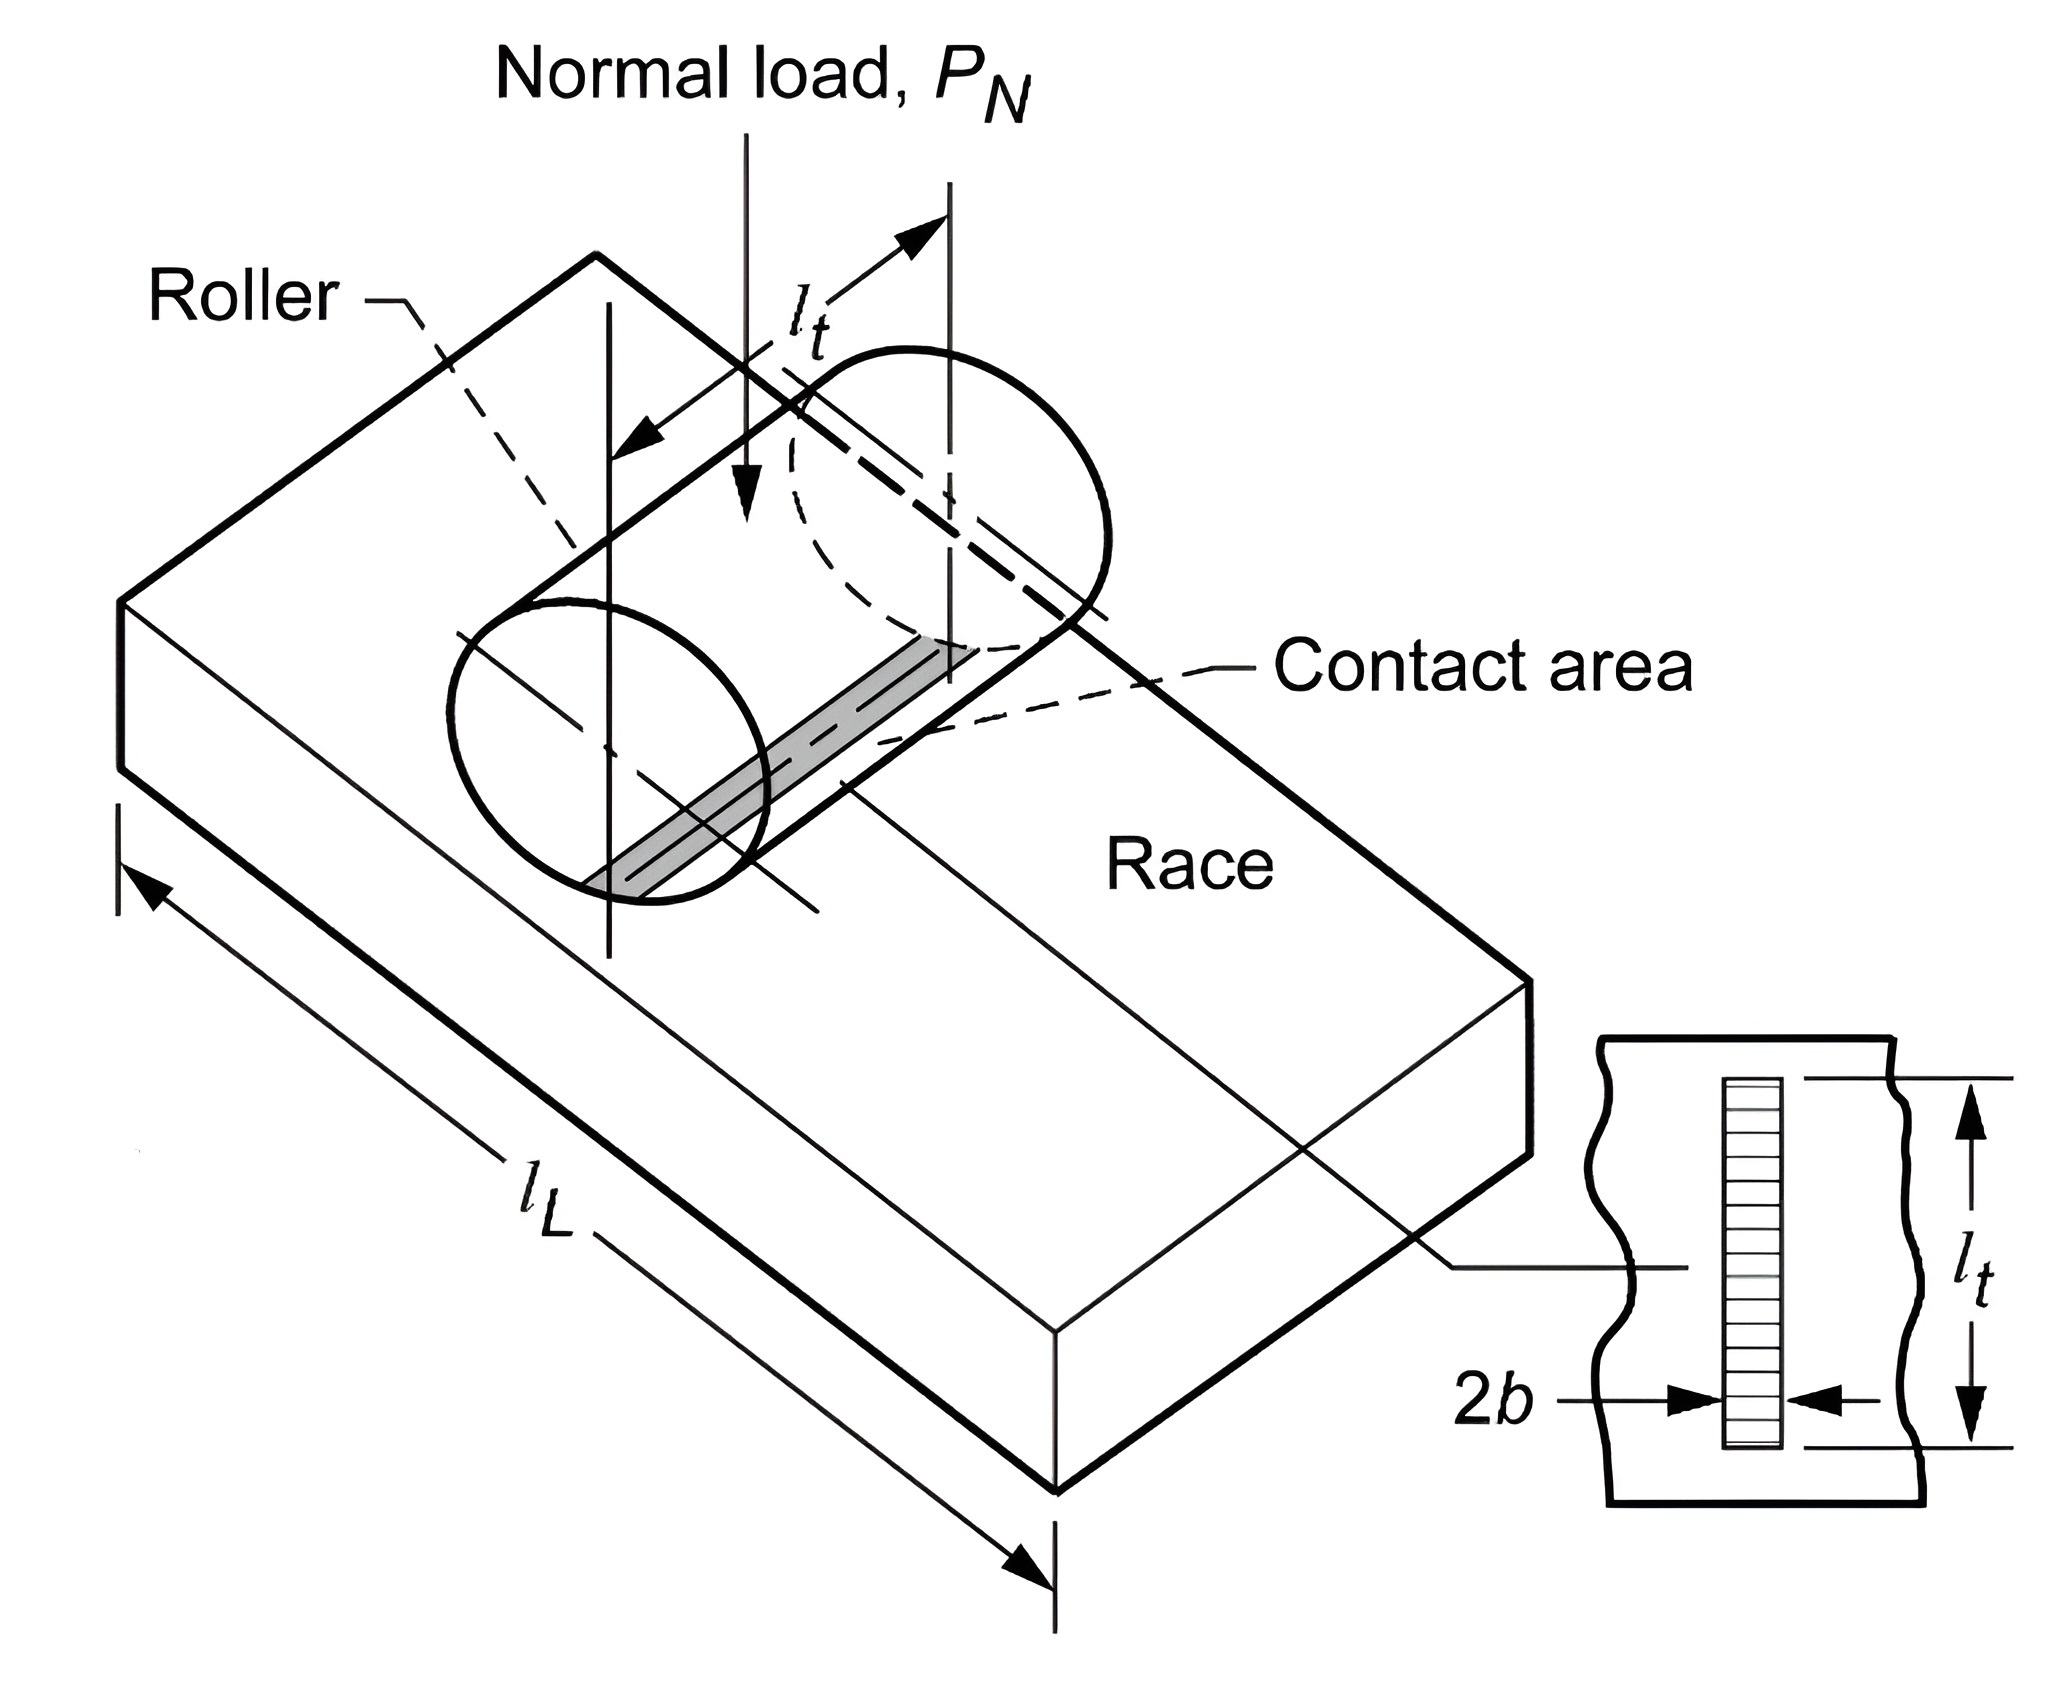
\includegraphics[width=125 mm]{LineContact.png}}
	\caption{Roller-race model for line contact \cite{Zaretsky2016}}
	\label{LineContact}
\end{figure}

\begin{figure}
	\centerline{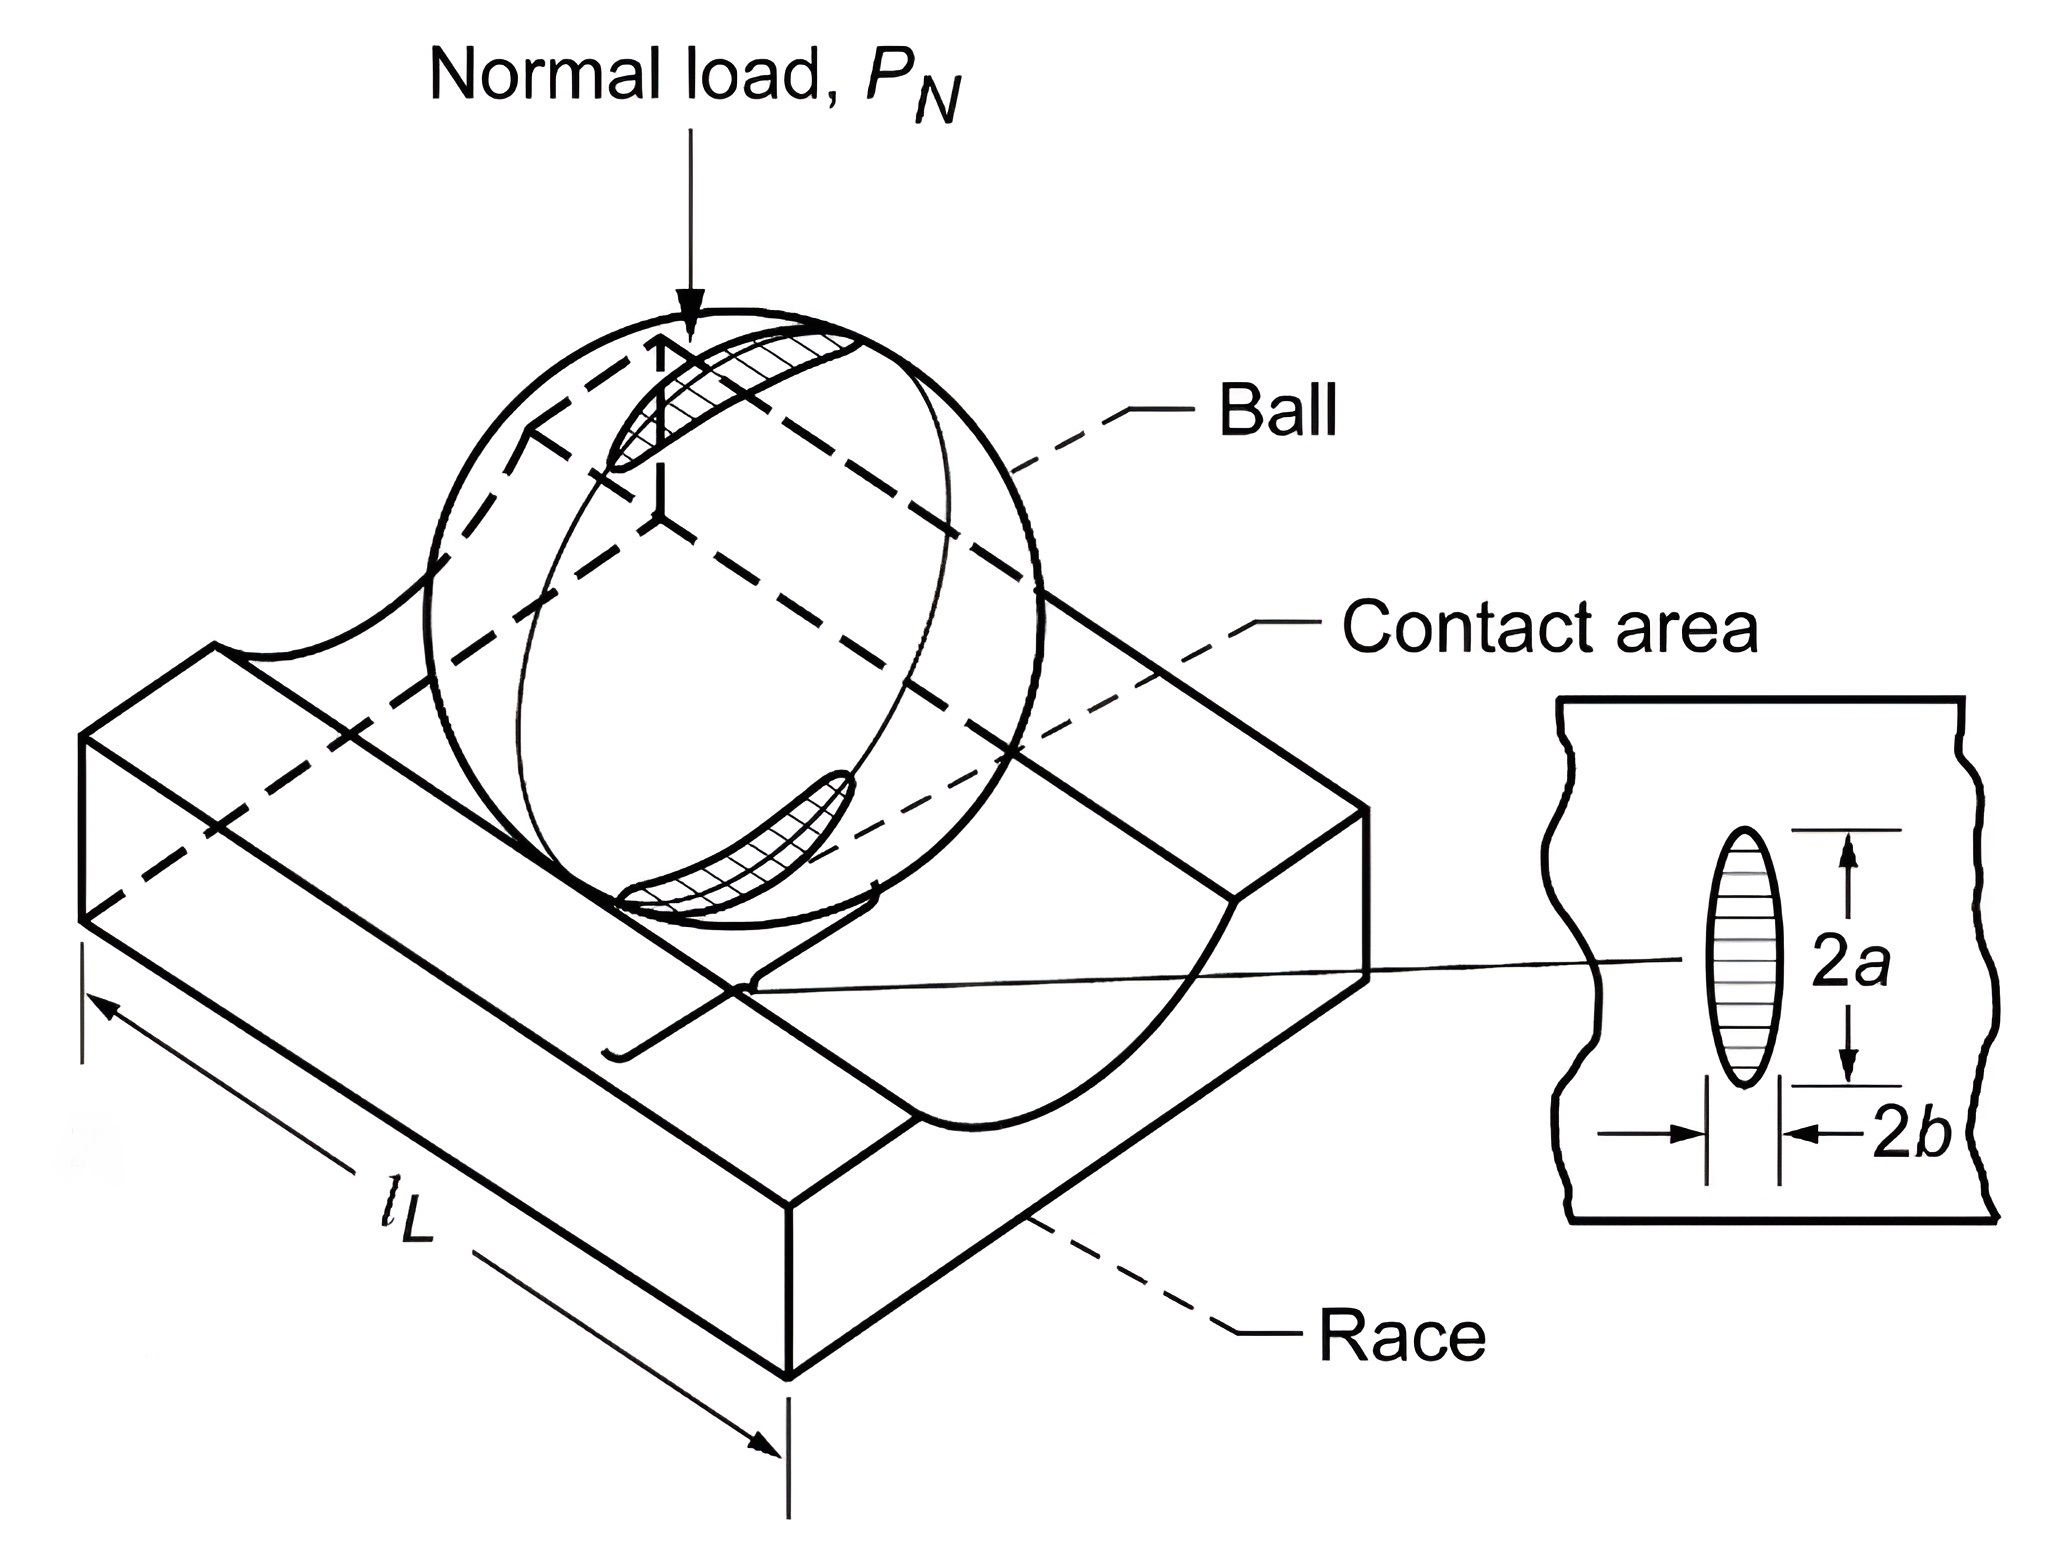
\includegraphics[width=125 mm]{PointContact.png}}
	\caption{Ball-race model for point contact \cite{Zaretsky2016}}
	\label{PointContact}
\end{figure}

Two cylinders with radii $R_1$ and $R_2$ contacting in a non-conformal manner can be simplified as a rigid cylinder in contact with an elastic half-space. This cylinder, as represented in Figure \ref{LineContact}, has a radius known as the reduced radius, $R^{\prime}$:

\begin{equation}\label{eq2.1}
	\frac{1}{R^{\prime}}=\frac{1}{R_1}+\frac{1}{R_2}
\end{equation}

The material properties of the two bodies are evaluated in a similar way. The elastic modulus, $E$ and Poisson's ratio, $v$, of both bodies are combined to calculate the reduced elastic modulus:

\begin{equation}\label{eq2.2}
	\frac{1}{E^{\prime}}=\frac{1}{2}\left(\frac{1-v_1^2}{E_1}+\frac{1-v_2^2}{E_2}\right)
\end{equation}

According to Hertz's theory of elastostatic solids in contact \cite{Hertz1881}, assuming the contact is frictionless, when load is applied to the cylinder it will experience very small strains. The amount that the cylinder deflects is much smaller than the radius of the cylinder, that is $\delta \ll R^{\prime}$. The total area of the contact is also much smaller than the radius of the cylinder $a \ll R^{\prime}$ (exaggerated in \ref{HertzianContactDeflection}). For example, a cylinder with a radius in order of $mm$ will have a contact width of a few tenths of a $mm$ and deflection a few tenths of a micron ( $\delta<a \ll$ $\left.R^{\prime}\right)$.

\begin{figure}
	\centerline{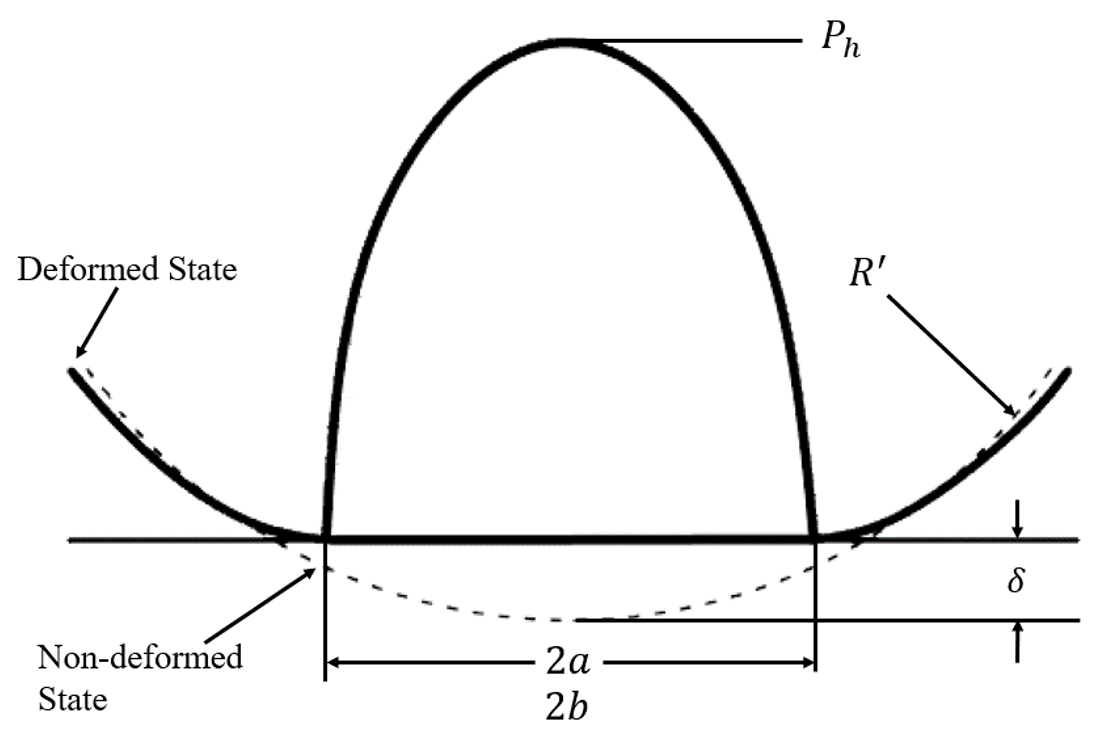
\includegraphics[width=100 mm]{Hertzian_Contact_Deflection.png}}
	\caption{Hertzian Contact Deflection}
	\label{HertzianContactDeflection}
\end{figure}

The value of the deflection determines the stiffness of the contact and the displacement of the inner bearing race with respect to the outer. The contact area determines the contact pressures and hence maximum sub-surface stresses. Excessive sub-surface stress could lead to inelastic deformation and subsequent fatigue spalling.

Analytical formulae provide a way of calculating the dimensions of the contact patch, $b$, and the resultant maximum Hertzian pressure, $P_h$ given a known force, $w$, material properties and geometry of bodies. For the case of the line contact these are:

\begin{equation}\label{eq2.3}
	b=\sqrt{\frac{8 w R_{z x}}{\pi E_r}}
\end{equation}

\begin{equation}\label{eq2.4}
	P_h=\sqrt{\frac{2 w}{\pi b}}
\end{equation}

where $w$ is load per unit length.

\section{Elastohydrodynamic Lubrication}

\subsection{History}

Under the EHL regime, both the elastic deformation of the solids in contacts as well as hydrodynamic theory are considered. Elastic bodies in contact for the case of ellipsoidal contacts was first investigated by Hertz in 1881 [6], allowing him to obtain the pressure distribution within an ellipsoidal contact. Separate studies on hydrodynamic lubrication were being performed by Reynolds in 1886 [7], based on a simplified version of the Navier-Stokes equation. It took a further 30 years before the two studies would be combined.

Early EHL studies began in 1916 when the pioneering work by Reynolds was applied to a simplified model of a gear-tooth contact by Martin [8]; replicated as two contacting cylinders. This analysis assumed that the solid bodies were rigid and the lubricant to behave with constant viscosity (ie. a hydrodynamic analysis). The resultant pressures were too high and the film thickness so low (1-10nm) that coverage of asperities (typical order of 100nm for machined gear teeth) was not possible. This contradicted experimental findings where machining tracks on high-speed gear tooth flanks were still visible after prolonged usage, which could only be explained by the presence of a sufficient lubricant film.

Between the 1930’s and 1950’s, significant research was performed to include both the elastic deformation of the surfaces and the effect of pressure on viscosity. Peppler [9] and Meldahl [10] both included the effects of surface deformation for non-conformal contacts, with Gatcombe [11] amongst others investigating viscosity increase due to the high pressure in the contact area. Typical EHL pressures are in the range of 0.5-4GPa and the resulting piezo-viscous properties were found to be partially instrumental to forming the film.

Considered the origin of EHL, Grubin’s pioneering work in 1949 [12] combined both elastic deformation and viscosity increase under pressure in film thickness calculations for the first time. In this analysis, he assumed that the deformed surface profiles in a highly loaded lubricated contact matched those produced in a classic dry Hertzian contact of the same materials and loading conditions. Reynolds equation could then be solved at the inlet region of the contact and a more accurate determination of the separation of the solids in the central region was found. This led to a film thickness in the predicted range (an order higher than Martin’s theory) and a more realistic pressure distribution than previous work. This pioneering study formed the basis for future EHL studies.

The first numerical solution of the line contact problem was presented shortly after by Petrusevich [13] which agreed with Grubin’s main conclusions. It contained the three main features of an EHL contact: a nearly parallel film in the contact zone with local constriction at the exit, a Hertzian pressure profile, and secondary local maximum pressure or ‘spike’ at the outlet (see Figure 6). In 1959, Dowson and Higginson [14] presented their numerical solution to the isothermal line contact EHL problem. Their iterative inverse method enabled the evaluation of film thickness and pressure distribution for line contact problems for lightly loaded cases. Throughout the 1960s, the authors investigated the effects of variables such as dimensionless surface velocity, materials parameter and load on EHL solutions. The authors then curve fitted their results and generated an empirical formula for isothermal line contacts [15], which was then improved upon by Dowson [16] and Dowson and Toyoda [17]. The formulae predict the minimum film thickness as a function of the rolling velocity, load and material parameters.

Empirical formulae are widely used today for analytical calculations that do not require the computational intensity of a full numerical solution. They are, however, somewhat limited to the operating parameters used in original simulations and do not offer the capabilities of a full numerical solution such as the modelling of inlet starvation at high speeds.

\subsection{Numerical Methods}

There are 2 main numerical methods for solving the elastohydrodynamic problem, direct and inverse. Typically, Reynolds equations is solved for pressure based on the lubricant film thickness. Early studies using this direct method suffered from convergence in highly loaded cases.

\paragraph{Inverse Method}

Ertel [18] introduced the inverse method for the hydrodynamic problem, which was adopted by Dowson and Higginson [14] for the EHL line contact problem. Here, the film thickness profile is found from a given pressure distribution. Solving the elastic deformation equation provides a second film thickness profile that corresponds to the same pressure distribution. This pressure distribution is then modified manually until the film thickness solutions converge.

This approach has many disadvantages. For low load cases with a non-parallel film shape in the contact region, this method is not suitable since the deviation of the Hertzian starting solution is too large. The film thickness equation is also insensitive to local variations in pressure. Finally, it is only suitable for line contact 1-dimensional cases since the Reynolds equation cannot be integrated for the two-dimensional case. Evans and Snidle [19] overcame the 2-dimensional limitation by using their quasi-static solution where a direct method was applied at the inlet zone and the inverse method in the contact zone. The aim was to overcome the instabilities of the forward iterative method to solve heavily loaded contacts which were limited to 0.5GPa, whereas common stresses in practice are typically in the order of 1.5GPa, reaching as high as 4GPa in some cases. A solution was only found for heavily loaded cases and the approach was limited by the need for an accurate initial estimate for pressure.

\paragraph{Direct Method}

The direct iterative method is the most common method whereby Reynolds equation is solved to find the pressure with a given film thickness. This pressure distribution is used with the elastic equation to calculate a new film shape. The pressure distribution must also achieve equilibrium with the externally applied load.

Two different direct methods have been used to solve the discretized Reynolds equation. The first is the iterative technique which has been applied to the 1-dimensional line contact problem [20] as well as the two-dimensional point [21] and elliptical [22] contact problem. The Gauss-seidel scheme was used, solving Reynolds equation for pressure based on film thickness and iterating between the two until convergence was met. Force equilibrium in an outer loop was calculated by integrating pressure across the contact domain and ensuring convergence between the resultant force and the applied external load. The solution comprises of 3 nested loops that must all converge. Underrelaxation between successive iteration is applied to aid convergence, however this iterative method does not converge for high loads. Furthermore, the number of iterations to achieve convergence is large (ie. of the square of the number of computational points used) and thus excessive computation times result.

The second solution method is the Newton-Raphson method. This was first applied by Okumara [23] and later by Houpert and Hamrock [24], where pressures as high as 4.8GPa were obtained with low CPU times. These low CPU times are a significant advantage of the NR methodology, with a smaller number of iterations resulting in much faster convergence than Gauss-Seidel.

Further numerical development came in the form of the multi-level method, first used by Lubrecht et al. in 1986 [25]. Venner et al. [26] used a multilevel multi-integration for point and line contacts in 1990 to reduce the computational cost of solving the film thickness integral. This allowed more nodes in the computational domain to be used for more complex problems with again much faster solution times. Finer grids could therefore be used, yielding faster results than NR for more complex cases with a solution time proportional to (n log n), with n being the total number of nodes in the computational domain. This work was mainly focussed on reducing computational time for the point contact problem, with the authors acknowledging the applicability of the Newton-Raphson numerical scheme for the line contact problem.

\subsection{Starvation}

The assumption of a fully flooded inlet region to the contact is not always valid. Starvation may occur if insufficient lubricant is entrained into the contact; significantly affecting EHL characteristics such as film formation and friction coefficient. This starvation is found to be greater at higher speeds, with higher viscosity lubricants and limited lubricant supply [27]. At high speeds, lubricant replenishment is diminished. For a fully flooded contact, the pressure builds upstream of the contact starting from a pressure gradient close to zero. With insufficient lubricant, the contacting bodies entrain two layers of lubricant, which then merge and form a meniscus at the contact inlet; causing the pressure rise to occur closer to the contact centre with a non-zero pressure gradient and reduced shape of the characteristic pressure distribution [28].

Analytical work on this topic began for the line contact problem by Wolveridge et al. [29] and later developed for the elliptical contact problem by Hamrock and Dowson [30]. In these studies, the inlet distance to the centre of the contact domain is varied as an input parameter. As the inlet distance is extended, the flooded condition at the entrance to the contact becomes greater. At a certain inlet distance, the film thickness in the contact is hardly affected (see Figure \ref{Starvation_Hamrock_Dowson}), and this is defined as the threshold between starvation and a fully flooded inlet condition. For the case of shorter inlet distances and subsequent starved condition, an equation was presented that could adjust the starved film thickness based on the starvation level and flooded film thickness.

\begin{figure}
	\centerline{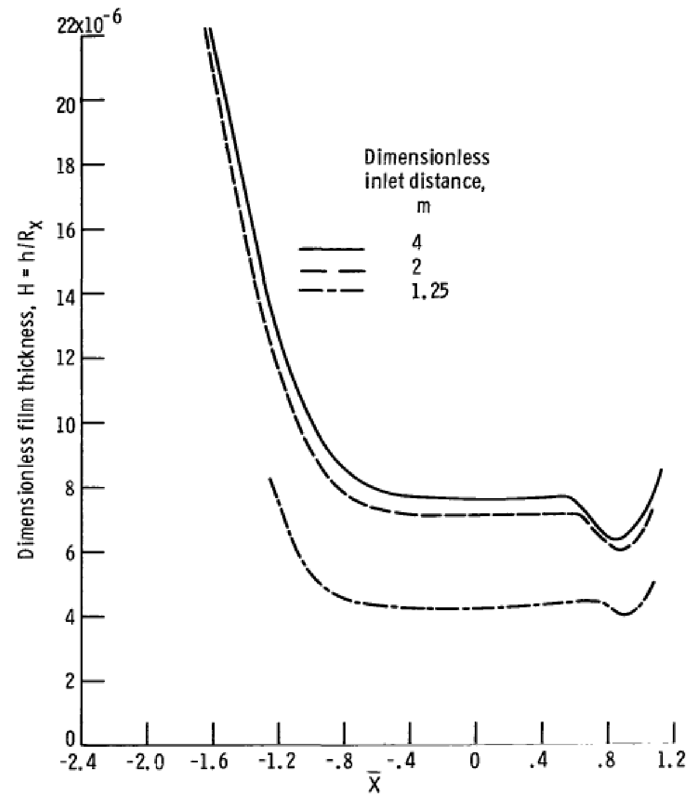
\includegraphics[width=125 mm]{Starvation_Hamrock_Dowson.png}}
	\caption{Effect of dimensionless inlet distance on film thickness for starvation modelling \cite{Hamrock1976}}
	\label{Starvation_Hamrock_Dowson}
\end{figure}

\subsection{Thermal EHL}

Heat is generated in an EHL contact in two ways: due to the viscous shearing of the lubricant and the compressive action of the generated pressures [31]. Classic EHL theory is isothermal and considers a Newtonian fluid with no temperature rise from sliding at the conjunction. For the case of pure rolling, this is sufficient to predict film thickness and inlet temperature rise. Rolling element bearings, however, undergo complex rolling and sliding motions depending on the nature of the loading and contact conditions. The presence of sliding requires a rheological model that considers the viscosity relationship with pressure as well as the use of the energy equation to calculate temperature rise within the lubricant film.

The three-dimensional energy equation has been solved by various authors for the line contact [32], point contact [33], [34] and finite line contact [35]. The generated heat is carried along the direction of entraining motion, in the direction of side leakage from the contact, and through the bounding surfaces of the contact. This can be reduced to fewer dimensions for the assumption of negligible heat transfer to the contacting bodies in the direction of the film thickness.

It has been found in the case of the point contact under low loads, thermal effects on pressure distribution and film thickness are negligible [36]. However, Kim and Sadeghi [33] concluded that with higher loads, the temperature rise in the film is significant. Under pure rolling conditions, the lubricant film temperature rise was only a moderate 15 °C above ambient and occurred at the inlet zone. As the slide/roll ratio was increased to 0.2, for the same load and speed conditions a temperature rise of 140 °C above ambient resulted at the contact centre, with the dominant mode of heat transfer being shear heating in the contact. The authors also adjusted the ellipticity parameter of the contact [34], with higher ellipticity parameters bringing the elliptical shape of the contact closer to that of a line. In this study, the load was more moderate, and the temperature rise for pure rolling and a slide/roll ratio of 0.2 was 4.5 °C and 16 °C respectively.

Habchi et al. [37] found that even under light loads and moderate speed conditions, thermal effects were still noticeable for Newtonian fluids. For lightly loaded cases, thermal and isothermal results were comparable up to entrainment velocities of 1 m/s but began to diverge slightly above this: in line with experimental findings. Additionally, as the slide/roll ratio is increased above 0.5, both central and minimum films are found to decrease for the thermal model, whereas the isothermal model remains constant. This is due to shear heating reducing lubricant viscosity. The difference was found to be only 0.015 μm between pure rolling and close to pure sliding for a lightly loaded contact.

Shear thinning of the lubricant also occurs at the inlet region to the contact. EHL films are micron level thickness, and assuming a fully flooded inlet, not all of the lubricant will traverse into the contact. Rejected lubricant will then produces some reverse flows which will shear the lubricant, increasing the inlet temperature and hence reduce the viscosity of the fluid [38].

It is therefore clear that the thermal elastohydrodynamic model is necessary for highly loaded conditions with modest slide/roll ratios.

\subsection{Elastohydrodynamic Pressure and Film Characteristics}

If there is relative velocity between two contacting surfaces, a thin film is formed due to the wedge mechanism and lubricant is entrained into the contact. The pressure profile across the contact deviates from the dry Hertzian parabolic distribution due to the presence of the lubricant.

Figure \ref{EHL_Film_Pressure_Schematic} shows the deviation of the film pressure from the dry Hertzian pressure. The main deviation occurs at the outlet of the contact due to the exit conditions. At the entry of the contact, the increasing pressure profile acts to oppose the flow of lubricant into the contact due to the entraining motion. At the outlet, the Couette profile and the pressure differential acts in the same direction to force lubricant out of the contact. For mass flow rate of the lubricant across the contact to be conserved, an outlet constriction is formed to reduce the flow area. The pressure spike at the outlet generates this deformation of the surfaces to maintain this flow balance and is a result of the piezo-viscosity of the lubricant. The two laws that must be obeyed are therefore the force equilibrium (the differential of pressure across the contact must equal the applied force), and the flow continuity.

\begin{figure}
	\centerline{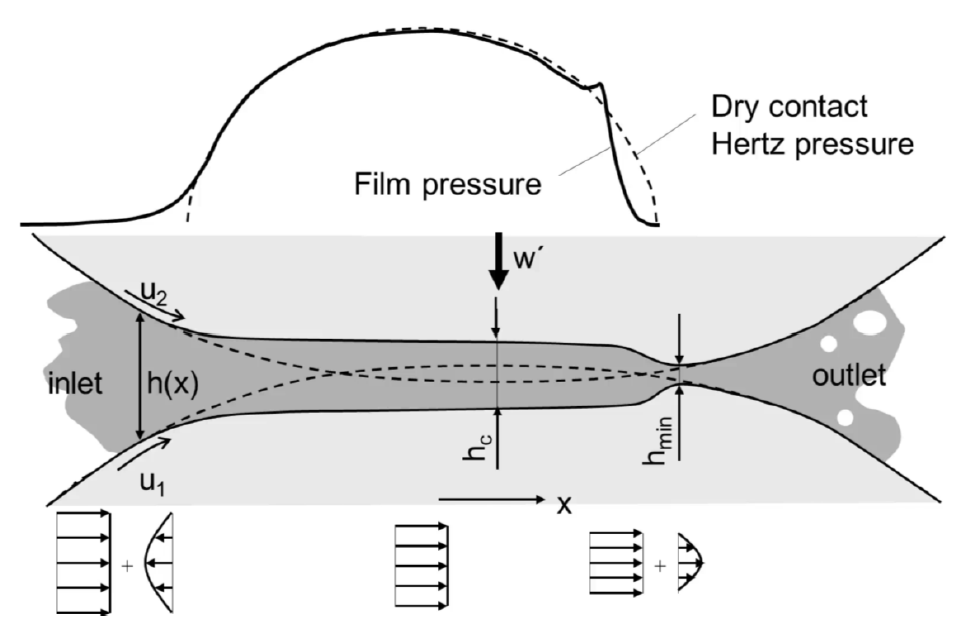
\includegraphics[width=125 mm]{EHL_Film_Pressure_Schematic.png}}
	\caption{EHL film and pressure distribution \cite{Larsson2013}}
	\label{EHL_Film_Pressure_Schematic}
\end{figure}

\subsection{Lubrication Regimes}

Lubricated contacts fall into four main regimes, these are:

\begin{itemize}
	\item \textbf{Hydrodynamic}: Contacting surfaces are completely separated by the lubricant film. Load is light, typically several Newtons. The contact surfaces do not experience deformation and resultant pressures are in the region of MPa.
	\item \textbf{Elastohydrodynamic}: Contacting surfaces are completely separated by lubricant film; however, load is medium to heavy. Contact deformation occurs and resultant contact pressures are in the region of GPa.
	\item \textbf{Mixed}: An interrupted oil film separates the two surfaces, ie. some asperity interaction occurs. Mixed lubrication can occur under any load and is dependent on the film thickness and asperity height.
	\item \textbf{Boundary}: The lubricant film is negligible, and surfaces directly interact. This a dry contact. At medium and high loads, Hertzian contact conditions can be assumed.
\end{itemize}

The loaded contact region of bearings are typically in the elastohydrodynamic regime of lubrication. The film thickness to asperity roughness height (lambda ratio) is large enough that the surface features do not typically influence the lubricant thickness and often a smooth surface is assumed. Under operation, emerging clearances result in unloaded regions of the bearing which can cause the roller-to-race contact to deviate from the elastohydrodynamic lubrication regime towards hydrodynamic regime, resulting in sliding and roller-cage collisions [31]. Hence, the contact may go through different regimes of lubrication throughout its rotation.

Film thickness and surface roughness are related by Stribeck [39] using the specific film thickness:

\begin{equation}\label{eq2.5}
	\lambda_s=\frac{h}{\sigma}
\end{equation}
 
 where $h$ is the lubricant film thickness and $\sigma$ is the roughness height of the asperities on the contact surfaces. Figure \ref{Stribeck_Curve} presents the various lubrication regimes and their associated coefficient of friction. For rougher surfaces, mixed-EHL occurs where contact of surface asperities occurs, increasing friction. The coefficient of friction then reduces as the film increases or asperity height reduces, until the hydrodynamic regime is reached, and the thicker films increase viscous friction.

\begin{figure}
	\centerline{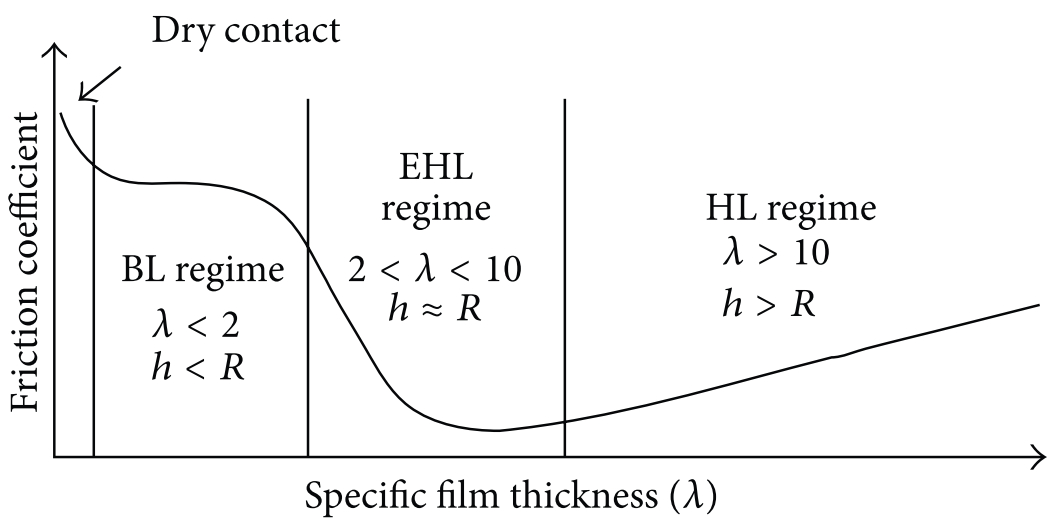
\includegraphics[width=125 mm]{Stribeck_Curve.png}}
	\caption{Stribeck curve and specific film thickness ($\lambda$) \cite{Ali2015}}
	\label{Stribeck_Curve}
\end{figure}

\chapter{Investigating the Effect of Lubrication on the Tribodynamic Behaviour of High-Speed Roller Bearings}
\label{Investigating the Effect of Lubrication on the Tribodynamic Behaviour of High-Speed Roller Bearings}


Prior to the development of the 6 DOF dynamic model, a high-speed experimental test rig was instrumented to obtain boundary conditions for subsequent tribological models. This work was performed to ascertain what type of models need to be developed in the tribology domain without the need for a dynamic model. The requirement for lubricated rather than dry contact models, regimes of lubrication and workflows such as implicit or explicit modelling have been investigated.

\section{Overall Workflow}

To obtain the film thickness at the roller-race contact, the load on each roller must be calculated implicitly based on the contact deflection. This is obtained conventionally from a dynamic model by solving the equations of motion, but these are currently lacking the required in-depth physics such as system flexibility, flexibility of races and thermal effects \cite{Matsubara1988} \cite{Wang2015} \cite{Liu2017c}.

To circumvent the need for a complex flexible dynamic model and to capture real behaviour of a bearing under test, displacement of the bearing centre and hence contact deflection is captured from experimental test results.

An experimental test rig is used to obtain the relative displacement between the inner and outer bearing races. Then, using the Hertzian load-deflection relationship and accounting for the lubricant film thickness, load on an individual roller is found at each instantaneous position around the bearing centre through a speed sweep of 0~–~15~000~$rpm$. An implicit analytical tribological model is used which calculates the film thickness at the contact. This loop is iterated to account for the tribodynamic coupling. After the experimentally informed implicit tribodynamic model is solved, load and speed values at specific rotational velocities are used within an explicit numerical EHL model to calculate film thickness and pressure distribution across the contact. The flow diagram in \ref{Experimental Tribodynamics Methodology Overview} illustrates the methodology used. Interactions between each stage will be explained in subsequent sections.

\begin{figure}
	\centerline{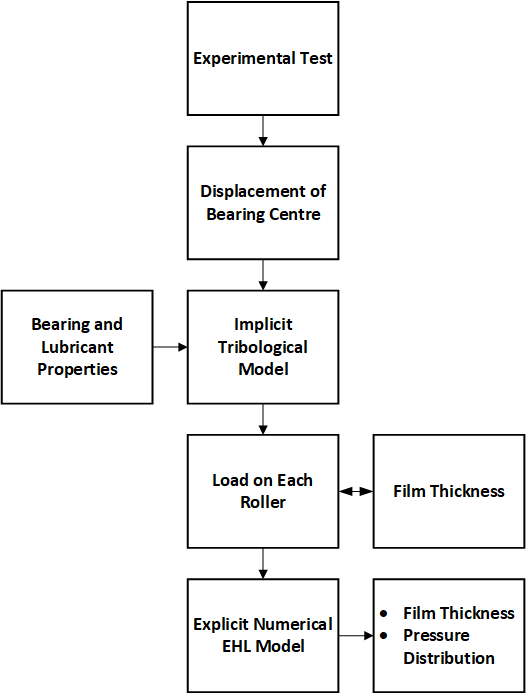
\includegraphics[width=100 mm]{ExpTribo Figure 1 - Methodology Overview.png}}
	\caption{Methodology Overview.}
	\label{Experimental Tribodynamics Methodology Overview}
\end{figure}

The rollers within a bearing carry an instantaneous share of the overall applied load \cite{Guo2020}. Deviation of the supported shaft centre from its nominal geometric centre results in a loaded region of the bearing. In the conjunction between the bearing roller and race, the non-conformal nature of contact generates very high pressures when under load. This causes local surface deformation and an increase in lubricant viscosity, resulting in EHL film formation \cite{Gohar1988} \cite{Grubin1949}. Emerging clearances in unloaded regions of the bearing results, which can cause the roller-to-race contact to deviate from the EHL regime towards the hydrodynamic regime, result in sliding and roller-cage collisions \cite{Mohammadpour2015c}. Hence, the contact may go through different regimes of lubrication throughout its rotation \cite{Denni2019}.

\begin{figure}
	\centerline{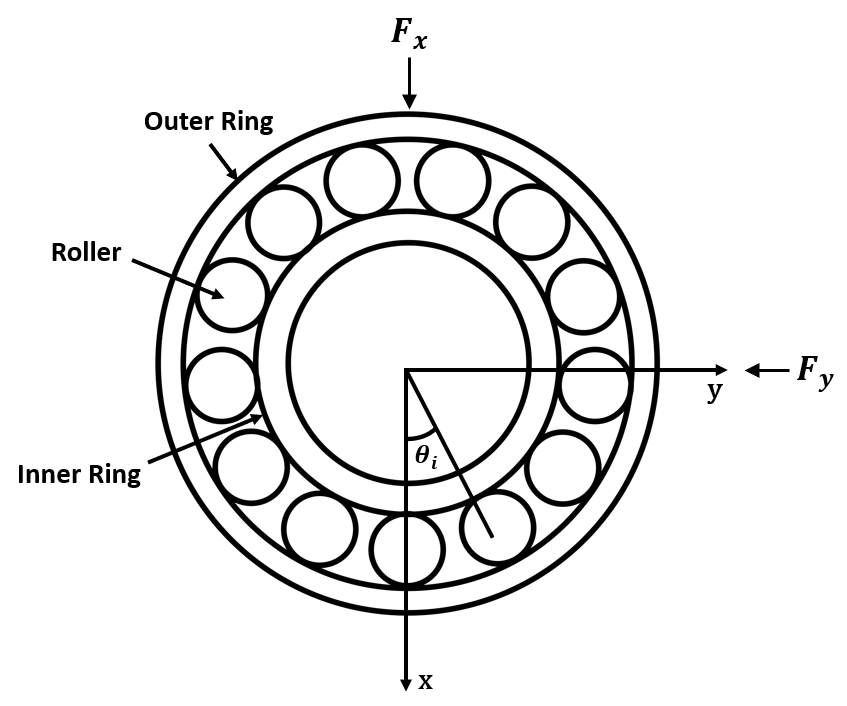
\includegraphics[width=100 mm]{ExpTribo Figure 2 - CRB in equilibrium position.png}}
	\caption{Cylindrical roller bearing in equilibrium position.}
	\label{CRB in equilibrium position}
\end{figure}

Figure \ref{CRB in equilibrium position} shows the cylindrical roller bearing (CRB) in equilibrium position with zero preload or design clearance. Under zero applied radial load, $F_0$, the initial deformation, $\delta_o$, and radial clearance, $C_0$, between rollers and races are both zero. Due to external force application and system dynamics, an instantaneous radial load, $F$, will displace the inner bearing race from its equilibrium state ($\Delta x$ and $\Delta y$). By analysing an individual roller at its instantaneous angular position, $\theta_i$, the resultant displacement of the bearing centre can be used to find deflection at the roller-race contact, $\delta_i$. These contact deformations will result in contact forces, $W_i$, which act to keep the rollers and races in dynamic equilibrium. The above interpretation is valid considering rigid inner and outer races.

\begin{figure}
	\centerline{\includegraphics[width=150 mm]{ExpTribo Figure 3 – Mutual separation and convergence of inner and outer races 2.png}}
	\caption{Mutual separation and convergence of inner and outer races.}
	\label{Mutual separation and convergence of inner and outer races}
\end{figure}

Figure \ref{Mutual separation and convergence of inner and outer races} presents the case whereby an instantaneous force is applied to the inner race. This causes deflection of the rollers in the loaded region and clearance around the rollers in the unloaded region. The value of the total deflection, $\delta_i$ at the inner and outer race corresponds to the component of displacement of the bearing centre at the instantaneous position of that particular roller. In the current study, this value was experimentally measured from the test rig and is used quasi-statically as the boundary condition for the tribological model. It should be noted that in-plane two degrees of freedom motion are analysed in this study which is a valid assumption under dominant radial loading with secondary horizontal motion from the full system dynamics. Misalignment along the length of the rollers is not considered due to the high stiffness of the shaft and bracket, hence a 1-dimensional analysis for EHL is sufficient \cite{Gupta1979}.

In the loaded region, the Hertzian load-deflection relationship is used to obtain the resulting instantaneous load on the roller. This value is then used implicitly within an analytical tribological model to calculate contact film thickness for an individual roller as it passes through different angular positions during a speed sweep. An extrapolated film thickness formula is used for this purpose. The calculated film thickness imposes additional deformation at the contact points which itself changes the calculated load. Hence, an iterative approach is required between the force calculation and implicit tribological model. In this part of the workflow, the stiffness and damping of the EHL film is neglected due to its rigid-like stiffness, which is several orders of magnitude higher than the Hertzian contact \cite{Dareing1975} \cite{Mehdigoli1990} TODO !!!USE LATEST REFERENCES FROM TRIBODYNAMIC PAPER.

For in-depth tribological investigations, the numerical solution of the fluid film is essential. This provides the pressure, film thickness and shear distributions in the contact to study the durability and frictional efficiency of the system. In the current study, the load on the roller and contact kinematics obtained from the implicit bearing model is used explicitly in a 1-dimensional elastohydrodynamic model to obtain film thickness and pressure distribution at the contact for specific loading periods through the speed sweep, as is shown in Figure \ref{EHL film thickness and pressure distribution at contact}. This explicit approach significantly improves the computational efficiency of the model and in principle, maintains the accuracy since only the central value of the film is required in the load calculation.

\begin{figure}
	\centerline{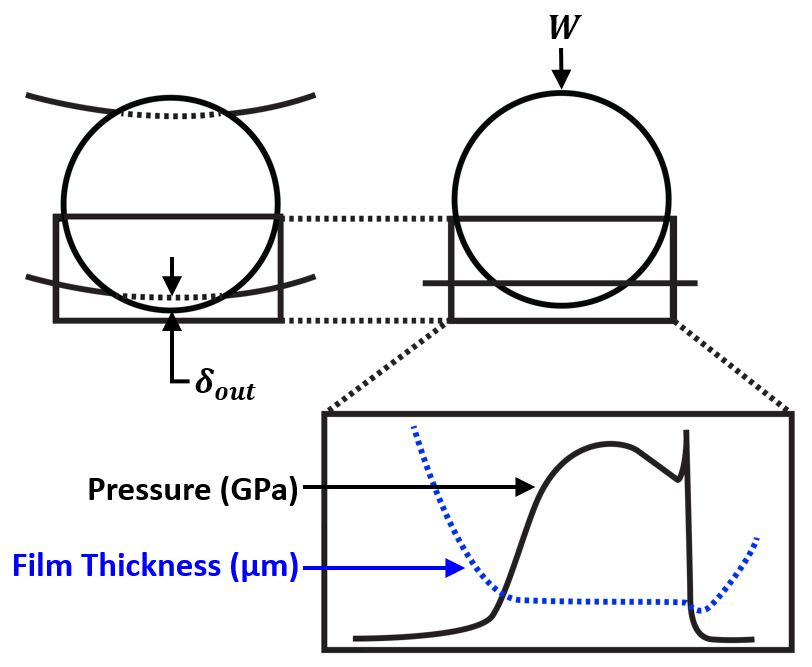
\includegraphics[width=100 mm]{ExpTribo Figure 4 - EHL film thickness and pressure distribution at contact.png}}
	\caption{EHL film thickness and pressure distribution at contact.}
	\label{EHL film thickness and pressure distribution at contact}
\end{figure}

\subsection{Experimental Test Rig}

The displacement of the bearing centre governs the conditions at the contact and was found experimentally using a high-speed bearing test rig, originally reported by Walker et al. \cite{Walker2018a}. A 5~kW AC synchronous motor, capable of speeds up to 32~000~rpm was coupled to a steel shaft that is supported by two bearing brackets. Radial force was transferred to inner bearing race via the shaft using a hinge/arm mechanism and a load application device on the shaft. Displacement data were obtained from an instrumented bearing bracket. Figure \ref{Experimental rig schematic} shows a schematic of the rig.

\begin{figure}
	\centerline{\includegraphics[width=120 mm]{ExpTribo Figure 5 – Experimental rig schematic.png}}
	\caption{Experimental rig schematic.}
	\label{Experimental rig schematic}
\end{figure}

The motor control unit was connected to a voltage input, transmitted via an NI cDAQ-9178 USB chassis for optimum resolution of the input voltage. A MATLAB script controlled the voltage ramp over a specified time-period and thus the spindle acceleration. In this study, a transient speed sweep was performed from 0~–~15~000~rpm in a 4~s period, with 750~N of static radial load applied to the shaft. The bearing under test was a single row cylindrical roller bearing, NU~205~ECP, located in an aluminium test bracket that had an extruded bore for instrumentation.

\subsection{Instrumentation}
The outer surface of the bearing bore was instrumented with two Type~4383 single-axis piezo-electric charge accelerometers, with a frequency range of 0.1~–~8.5~kHz and sensitivity of 3.16~pC/ms2.  These measured acceleration of the bracket’s bore, corresponding to the outer race of the bearing (Figure \ref{Accelerometer locations on test bracket}). Two single beam laser vibrometers measured the displacement of the shaft at the edge of the bearing which corresponds to the displacement of the inner race of the bearing (Figure \ref{Laser vibrometer locations on shaft}). A dual-beam vibrometer was used to measure the rotational speed of the shaft. All laser vibrometers had a frequency range of 0~–~10~kHz and maximum speed of 20~000~rpm.

\begin{figure}
	\centerline{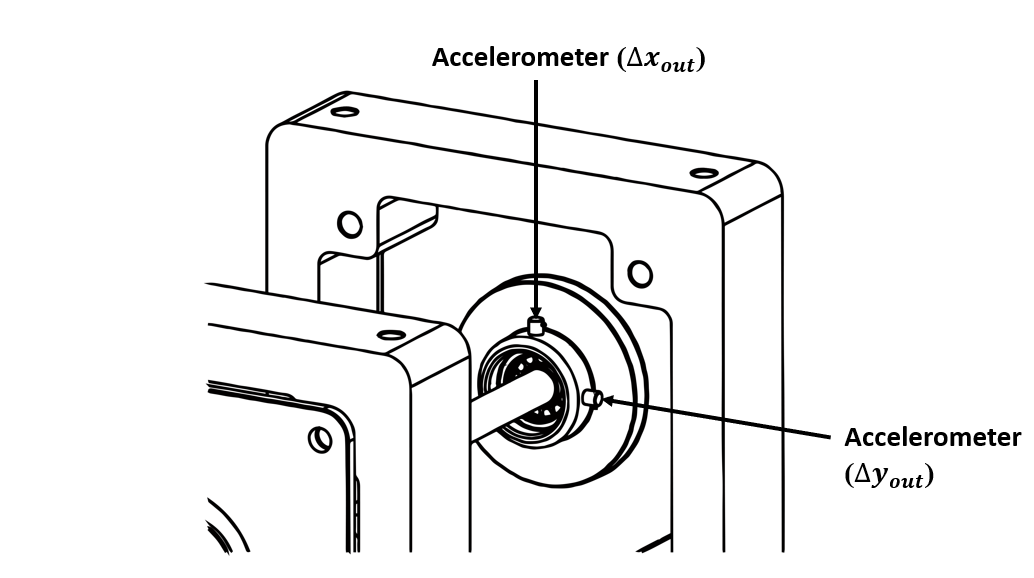
\includegraphics[width=150 mm]{ExpTribo Figure 6(a) - Accelerometer Locations on Test Bracket.png}}
	\caption{Accelerometer locations on test bracket.}
	\label{Accelerometer locations on test bracket}
\end{figure}

\begin{figure}
	\centerline{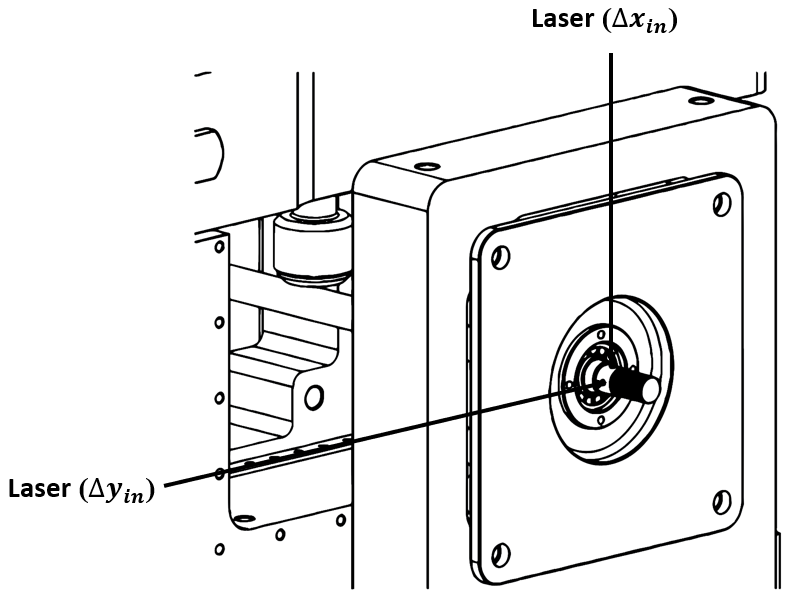
\includegraphics[width=120 mm]{ExpTribo Figure 6(b) Laser Vibrometer Locations on Shaft 2.png}}
	\caption{Laser vibrometer locations on shaft.}
	\label{Laser vibrometer locations on shaft}
\end{figure}

A program in MATLAB controlled the speed of the shaft through a ramped voltage input. Data was simultaneously acquired from the accelerometers and laser vibrometers through synchronised input channels at a sampling rate of 100~kHz. Simultaneous control and data acquisition ensure accurate results between different instrumentation locations.

\subsection{Signal Processing}
The bearing race displacements were obtained from the instrumented bearing using time-domain data from the accelerometers and laser vibrometers. The laser vibrometer directly provided displacement data, whereas the accelerometer data required post-processing of acceleration data. To ascertain the displacement of the bearing bore and thus outer bearing race, the accelerometer results were integrated twice:

\begin{equation}\label{accelvelointeg}
	v_{out}\left(t\right)=v_{0,out}+\ \int_{0}^{t}{a_{out}\ dt}
\end{equation}

\begin{equation}\label{acceldispinteg}
	x_{out}\left(t\right)=x_{0,out}+\int_{0}^{t}{v_{out}\ dt}
\end{equation}

As this double integration amplifies non-linearities in the original signal, it requires pre-processing \cite{Takeda2014}. Low frequency drift is removed from the unfiltered time-domain data by applying a linear fit to the data and then removing the trend from it.  

To extract the frequency content of the speed ramp, waterfall plots were generated using the accelerometer and laser vibrometer data. Short-time fast-Fourier transform (STFFT) was used, with data windows of six shaft rotations at each 100~rpm increment. The resulting signal was then filtered using a Butterworth bandpass filter for a frequency range of 70~-~10~000~$Hz$ to remove the high amplitude low frequency noise that was inherent to the equipment setup. The filter used 3~$dB$ of passband ripple and 7~$dB$ attenuation in the stopbands, which were set at 35~-~12~500~$Hz$.  
The relative displacement of the bearing centre could then be obtained from the relative displacement between the shaft (measured using the single beam laser vibrometer) and bearing bore:

\begin{equation}\label{relativdispaccelx}
	\Delta x = \Delta x_{in} - \Delta x_{out}
\end{equation}

\begin{equation}\label{relativdispaccely}
	\Delta y = \Delta y_{in} - \Delta y_{out}
\end{equation}

where $\Delta x_{in}$ and $\Delta x_{out}$ correspond to the displacements of the shaft and bearing bore respectively. 

\subsection{Contact Mechanics at the Roller Race Conjunction}

The contact between roller and race is modelled as an elastic deformation between an equivalent finite length elastic cylinder and rigid plate. This assumption is realistic under the conditions of an EHL contact. The contact force on an individual roller at each instantaneous position, $W_i$, is obtained from the Hertzian load-deflection relationship:

\begin{equation}\label{Hertz load deflection}
	W_i=k \delta_i^n
\end{equation}

where $k$ is the Hertzian contact stiffness non-linearity between a rolling element and the inner or outer raceway groove. For the case of rolling element bearings, the exponent of localised deflection, $n$, is equal to $10/9$ \cite{Harris1984}. The contact deflection of a roller relative to the race, $\delta_i$, is due to the normal dynamic motion (i.e. the local mutual convergence) of the inner and outer bearing races, contribution of lubricant film thickness and any additional clearance or interference fit \cite{Mohammadpour2015c}. This is expressed as:

\begin{equation}\label{Contact deflection experimental}
	\delta_i=2\left(h_{c,i}-C\right)+x\cos{\left(\theta_i\right)}+y\sin(\theta_i)
\end{equation}

where $C$ is the local radial clearance, and $x$ and $y$ are the displacement components of the inner bearing race from its geometric centre. This normal approach between both races is the sum of the total deformation of the rollers and both races \cite{Hamrock1981}, hence:

\begin{equation}\label{Total deflection experimental}
\delta_i=\ \delta_{i,in}+\delta_{i,out}
\end{equation}

The equilibrium of forces in a system of stiffnesses in series is therefore:

\begin{equation}\label{Equilibrium of force experimental}
W_i=W_{i,out}=W_{i,in}
\end{equation}

To find the individual deflection of each contact due to differences in contact stiffness, the following relationship is used:

\begin{equation}\label{Individual deflection of contacts experimental}
{\delta_{i,in}}^nk_i={\delta_{i,out}}^nk_{out}
\end{equation}

The deflection value at each contact based on the total deflection and relationship between contact stiffness is then found from Equations \ref{Total deflection experimental} and \ref{Individual deflection of contacts experimental} to give:

\begin{equation}\label{Deflection at each contact}
	\delta_{i, \text { out }}=\frac{\delta_i}{\left(\frac{k_{\text {out }}}{k_{\text {in }}}\right)^{\frac{1}{n}}+1}
\end{equation}

The normal stiffness of the inner and outer races differs due to their geometry. To calculate the stiffness at each contact, the following equation is used: 

\begin{equation}\label{Contact stiffness experimental}
	\delta=\frac{F}{\pi E_r L}\left[\ln \left(\frac{4 \pi E_r R_{z x} L}{F}\right)-1\right]
\end{equation}

The deflection for a range of loads is calculated based on the geometry and material properties at the inner and outer race contacts. This non-linear relationship is numerically obtained and then curve fitted and represented by a power function in the form $F=a\delta^b$, with $b=10/9$ and a representing the contact stiffness. Individual contact stiffness and deflection at the inner and outer race contacts is then found. The overall contact stiffness, $K_{i,total}$, is given by:

\begin{equation}\label{Overall contact stiffness}
	K_{i, \text { total }}=\frac{1}{\left(\frac{1}{K_{i, \text { in }}}\right)+\left(\frac{1}{K_{i, \text { out }}}\right)}
\end{equation}

where $K_{i,in}$ and $K_{i,out}$ are the stiffnesses of the inner and outer race contacts respectively.

\subsection{Implicit Tribological Model}

A stepwise solution was performed on an individual roller as it passes through each angular position. The roller bearing and bracket tolerances are such that the internal clearance is $0 \mu m$ between roller and race. This means that in an unloaded state, there is no deflection of elements or raceway. It also means that displacement in positive x-y corresponds to the same total magnitude of deflection of roller and race contact. For each time step, the bearing is first assumed to be in equilibrium position, and film thickness is assumed to be $0 \mu m$. The deflection of the bearing is calculated under these conditions and is therefore a function of the relative displacement between inner and outer bearing races. With deflection at the time step calculated, the resultant lubricant regime and subsequent analytical solutions can be performed based on the following three conditions:

\begin{enumerate}
	\item $\delta=0$ indicates a film of 0 $\mu m$ and no load.
	\item $\delta<0$ indicates complete separation of the roller and race. In this instance, the lubricant is assumed to fill the separation gap, with the film thickness value equalling the magnitude of the separation:
	
	\begin{equation}\label{hydrodynamic film thickness}
		h_i=\left|\delta_i\right||
	\end{equation}

	Under this condition, the lubrication is in the hydrodynamic regime. The hydrodynamic lubricant reaction load was derived by Rahnejat \cite{Rahnejat1984}, and is given by:
	
	\begin{equation}\label{hydrodynamic reaction load}
		W_i=\frac{2 b u_i \eta_0 R_{z x}}{h_i}
	\end{equation}

	where $b$ is the half length of the contact, $u$ is the speed of lubricant entrainment into the contact, $\eta_0$ is the lubricant viscosity, $R_{zx}$ is the reduced radius of the roller and race and $h$ is lubricant film thickness. 
	
	\item $\delta>0$ indicates deflection at the roller-race contact. This means that contact pressure is sufficiently high for the lubrication regime to be elastohydrodynamic. For the elastohydrodynamic regime, an iterative process is performed to solve film thickness. This is due to the contribution of EHL film towards deformation and consequently the load in the contact.
	
	The cylindrical roller and race contacts are modelled by an equivalent rigid roller against a semi-infinite elastic half space of equivalent elastic modulus, $E_r$. The extrapolated central film thickness for a line contact is therefore obtained \cite{Dowson1979} from:  
	
	\begin{equation}\label{dimensionless central film thickness}
	h_c=R_{zx}\left[{3.06G}^{\ast0.56}{U^{\ast0.69}W}^{\ast-0.1}\right]
    \end{equation}

	where the following dimensionless parameters are used:
		
	\begin{equation}\label{Gstar}
		G^*=\alpha E_r 
	\end{equation}
	
	\begin{equation}\label{Ustar}
		U^*=\frac{u \eta_0}{R_{z x} E_r}
	\end{equation}
	
	\begin{equation}\label{Wstar}
		W^*=\frac{w}{L E_r R_{z x}}
	\end{equation}

	where $R$ is the reduced radius of the contact, $L$ is the length of the roller and $u$ is the speed of entraining motion into the contact and $W$ is the contact load. Assuming pure rolling, the speed of entraining motion is given by:
	
	\begin{equation}\label{entraining motion speed}
		u_i=\frac{1}{2}\left(\omega_{c, i}-\omega_{r i, i}\right) r_{i n}
	\end{equation}

	An iterative process is used to calculate load on the roller based on total deflection including lubricant film (Equation \ref{Contact deflection experimental}). At each time step where an EHL film is present, the following convergence criteria must be met before the next time step is calculated:
	
	\begin{equation}\label{film convergence}
		\frac{h_i^n-h_i^{n-1}}{h_i^{n-1}} \leq 0.01
	\end{equation}

\end{enumerate}

\subsection{Friction Calculations}
Frictional power is a crucial factor for characterising their performance. Under modern high-speed conditions, it is important to also understand the frictional behaviour of the system. Roller bearings often operate within the mixed elastohydrodynamic regime of lubrication. Friction is generated by a combination of viscous shear of the lubricant and asperity interactions. Total friction at the mixed-EHL contact is a combination of the boundary friction, $f_b$, and hydrodynamic or viscous friction, $f_v$:  

\begin{equation}\label{Total friction experimental}
	f=f_v+f_b
\end{equation}

Boundary friction is a function of asperity contact pressure, calculated using the Greenwood and Tripp model in this paper \cite{Greenwood1970}:

\begin{equation}\label{Boundary friction experimental}
	f_b=\tau_0 A_a+\varsigma W_a
\end{equation}

where $\tau_0$ is the Eyring shear stress of lubricant and $\varsigma$ is the pressure coefficient for shear strength of asperities, obtained from asperity level friction measurement. Asperity load, $W_a$, and area occupied by asperities within the apparent contact $A_a$ are obtained as below, assuming a Guassian distribution of asperity peak counts: 

\begin{equation}\label{Asperity load}
	W_a=\frac{16 \sqrt{2}}{15} \pi(\zeta \kappa \sigma)^2 \sqrt{\frac{\sigma}{\kappa}} E_r A_a F_{5 / 2}(\lambda)
\end{equation}

and

\begin{equation}\label{Asperity area}
	A_a=\pi^2(\zeta \kappa \sigma)^2 A F_2(\lambda)
\end{equation}

where $\lambda=\frac{h}{\sigma}$ is the Stribeck parameter and $F_{5 / 2}(\lambda)$ and $F_2(\lambda)$ are statistical functions obtained from numerical integration of the Guassian distribution of asperities.  

Viscous Friction due to shearing of the lubricant film in the EHL contact is found using the below experimentally validated formulae \cite{Evans1986}:

\begin{equation}\label{Viscous friction Evans and Johnson}
	f_v=\mu W
\end{equation}

where

\begin{equation}\label{Viscous friction Evans and Johnson mu}
	\mu=0.87 \alpha \tau_0+1.74 \frac{\tau_0}{\bar{p}} \ln \left[\frac{1.2}{\tau_0 h}\left(\frac{2 K \eta_0}{1+9.6 \xi}\right)^{\frac{1}{2}}\right]
\end{equation}

where $\bar{p}$ is the average pressure at the apparent contact, $K$ is the lubricant thermal conductivity and $\xi$ is given by:

\begin{equation}\label{Viscous friction Xi}
	\xi=\frac{4}{\pi} \frac{K}{h / R_{z x}}\left(\frac{\bar{p}}{E_r R_{z x} K \rho^{\prime} c^{\prime} u}\right)^{\frac{1}{2}}
\end{equation}

where $K^{\prime}$, $\rho^{\prime}$ and $C^{\prime}$ are respectively the thermal conductivity, density, and specific heat capacity of the contacting solid. 

To inform the boundary friction model, surface topography data are required. An Alicona InfiniteFocus Variation Microscope with a $\times 10$ objective was used for topography measurements to calculate the roughness parameter, $n\sigma\beta$. This had a vertical resolution of 30 $nm$ and sampling point separation of 176.9 $nm$ in the $y-z$ plane of the roller and 1 $nm$ in $x$. An area of 530 by 588 $\mu m$ was captured. Data was processed using Vision65 Map Premium, where the profile of the radius of the roller was removed. The measured parameters are presented in Table \ref{Surface Topography Data}

\begin{table*}
	%\captionsetup{justification=centering}
	\caption{Surface Topography Data}
	\label{Surface Topography Data}
	\centering
	\renewcommand{\arraystretch}{1.5}%
	\begin{tabular}{|c|c|}
		\hline
		\ \textbf{Parameter} & \textbf{Value} \\ [0.5ex]
		\hline
		Root-mean-square height & 0.197 $\mu m$ \\ [0.5ex]
		\hline
		Density of peaks & 0.00116 $1 /(\mu \mathrm{m})^2$ \\ [0.5ex]
		\hline
		Arithmetic mean peak curvature & 0.180 $1 / \mu \mathrm{m}$ \\ [0.5ex]
		\hline
	\end{tabular}
\end{table*}

\section{Numerical EHL Model}\label{1D EHL Model}

Whilst the analytical solution used in the implicit tribological model provides central film thickness, the film thickness and pressure distributions can only be obtained explicitly through the full solution of Reynolds equation in conjunction with rheological and elastic field models. In a line contact, where contact dimensions in the side-leakage direction ($y_c$) are much larger than the direction of entraining motion ($x_c$), pressure in $y_c$ direction is assumed constant due to the negligible gradient and the contact can be analysed in one dimension. This assumption is valid in the contact apart from small regions near the edge. Reynolds equation is used to calculate contact pressures.

\subsection{Reynolds Equation}

Reynold’s equation \cite{Reynolds1886} is the governing equation of fluid film lubrication theory. For Newtonian fluids it can be derived from the full Navier-Stokes equations making the following assumptions, primarily the neglection of inertial forces and only retaining viscous forces on the lubricant \cite{Gohar1988}:
\begin{enumerate} % REQUIRES DIRECTIONS ADDING
	\item Body forces are negligible (mass of film is negligible)
	\item Pressure is constant through the lubricant film (z-direction) due to thin film (dimensions of the region of pressure are typically 100 times the central film thickness).
	\item No slip at boundaries
	\item Lubricant flow is laminar (low Reynolds number)
	\item Inertia and surface tension forces are negligible compared with viscous forces (working fluid has low mass and low acceleration)
	\item Shear stress and velocity gradients are only significant across the lubricant film %ADD DIRECTION OF THIS!!!!
	\item The lubricant behaves as a Newtonian fluid
	\item Lubricant viscosity in constant across the film %ADD DIRECTION!!!
	\item The lubricant boundary surfaces are parallel or at a small angle with respect to each other
\end{enumerate}

Reynolds equation is a second order, non-linear partial differential equation. It is made up of the pressure induced terms (Poiseuille flow) and the boundary velocity-induced term (Couette flow). 

For the line contact problem, such as that at the conjunction between a cylindrical roller and race, dimensions in the side-leakage direction,$y$, are much bigger than the direction of entraining motion, $x$. Pressure in $y$ direction is assumed constant due to the negligible gradient, and the contact can be analysed in 1-dimension. The assumption is valid in the contact apart from small regions near the edge where the roller profile changes. A simplified 1-dimensional version of Reynolds equation can therefore be used:

\begin{equation}\label{eq3.1}
	\frac{\partial}{\partial x}\left[\frac{\rho h^{3}}{6 \eta}\left(\frac{\partial p}{\partial x}\right)-\rho h u\right]=2 \frac{\partial(\rho h)}{\partial t}
\end{equation}

To solve Reynolds equation numerically, it must first be discretized and then solved using the finite-difference method. The following procedure explains this discretization.

Due to the steady state nature of the investigations, with the absence of shock loading, the transient squeeze term can be removed:
\begin{equation}\label{eq3.2}
	\frac{\partial}{\partial x}\left[\frac{\rho h^{3}}{6 \eta}\left(\frac{\partial p}{\partial x}\right)-\rho h u\right]=0
\end{equation}

Due to the many orders of magnitude differences between lubricant film thickness (µm) and pressures (GPa), the numerical solution often becomes unstable. Dimensionless parameters are therefore defined to remove this instability. These are as follows:

\begin{equation}\label{eq3.3}
	\begin{aligned}
		U &=\frac{u}{u_{a v}} & \partial x &=a \partial X \\
		\mathrm{X} &=\frac{x}{\mathrm{a}} & \partial \rho &=\rho_{0} \partial \bar{\rho} \\
		\bar{\rho} &=\frac{\rho}{\rho_{0}} & \partial \eta &=\eta_{0} \partial \bar{\eta} \\
		\bar{\eta} &=\frac{\eta}{\eta_{0}} & \partial h &=\frac{a^{2}}{R_{z x}} \partial H \\
		\mathrm{H} &=\frac{h R_{x}}{a^{2}} & \partial p &=p_{h} \partial P \\
		\mathrm{P} &=\frac{p}{p_{h}} & \\
		\mathrm{~W}^{*} &=\frac{w}{E_{r} R_{z x} L} &
	\end{aligned}
\end{equation}

Terms in the simplified Reynolds equation are replaced with dimensionless parameters. Similar terms are then grouped and rearranged to give the final form:

\begin{equation}\label{eq3.4}
	\frac{\partial}{\partial X}\left[\frac{\bar{\rho} H^{3}}{6 \bar{\eta}}\left(\frac{\partial P}{\partial X}\right)\right]=\Psi\left[\frac{\partial}{\partial X} \bar{\rho} H U\right]
\end{equation}

where

\begin{equation}\label{eq3.5}
	\Psi=\frac{12 u_{a v} R_{z x}^{2} \eta_{0}}{p_{h}}
\end{equation}

Grouping terms for simplicity
\begin{equation}\label{eq3.6}
	M=\frac{\bar{\rho} H^{3}}{6 \bar{\eta}}
\end{equation}

\begin{equation}\label{eq3.7}
	Q=\bar{\rho} H
\end{equation}

Making substitutions
\begin{equation}\label{eq3.8}
	\frac{\partial}{\partial X}\left[M\left(\frac{\partial P}{\partial X}\right)\right]=\Psi \frac{\partial}{\partial X}[Q U
\end{equation}

\begin{equation}\label{eq3.9}
	\left[M \frac{\partial^{2} P}{\partial X^{2}}+\left(\frac{\partial M}{\partial X}\right) \frac{\partial P}{\partial X}\right]=\Psi\left[U \frac{\partial Q}{\partial X}+Q \frac{\partial U}{\partial X}\right]
\end{equation}

The final term is removed, as velocity, $U$, is independent of $x$ when no stretching of the surfaces occurs. This is then differentiated to give:

\begin{equation}\label{eq3.10}
	\frac{\partial M}{\partial X}=\frac{\partial}{\partial X}\left[\frac{\bar{\rho} H^{3}}{6 \bar{\eta}}\right]=\frac{H^{2}}{2 \bar{\eta}}\left[\left(\frac{H}{3}\right) \frac{\partial P}{\partial X}+\bar{\rho} \frac{\partial H}{\partial X}-\left(\frac{\bar{\rho} H}{2 \bar{\eta}}\right) \frac{\partial \bar{\eta}}{\partial X}\right]
\end{equation}

and

\begin{equation}\label{eq3.11}
	\frac{\partial Q}{\partial X}=\frac{\partial}{\partial X}[\bar{\rho} H]=H \frac{\partial \bar{\rho}}{\partial X}+\bar{\rho} \frac{\partial H}{\partial X}
\end{equation}

Substituting into Equation \ref{eq3.9} gives the following:

\begin{equation}\label{eq1.12}
	\frac{\bar{\rho} H^{3}}{6 \bar{\eta}} \frac{\partial^{2} P}{\partial X^{2}}+\frac{H^{2}}{2 \bar{\eta}}\left[\frac{H}{3} \frac{\partial \bar{\rho}}{\partial X}+\bar{\rho} \frac{\partial H}{\partial X}-\frac{\bar{\rho} H}{2 \bar{\eta}} \frac{\partial \bar{\eta}}{\partial X}\right] \frac{\partial P}{\partial X}-\Psi U\left[H \frac{\partial \bar{\rho}}{\partial X}+\bar{\rho} \frac{\partial H}{\partial X}\right]=0
\end{equation}

\begin{equation}\label{eq3.13}
	\frac{\partial^{2} P}{\partial X^{2}}+\frac{3}{\bar{\rho} H}\left[\frac{H}{3} \frac{\partial \bar{\rho}}{\partial X}+\bar{\rho} \frac{\partial H}{\partial X}-\frac{\bar{\rho} H}{2 \bar{\eta}} \frac{\partial \bar{\eta}}{\partial X}\right] \frac{\partial P}{\partial X}-\frac{6 \bar{\eta}}{\bar{\rho} H^{3}} \Psi U\left[H \frac{\partial \bar{\rho}}{\partial X}+\bar{\rho} \frac{\partial H}{\partial X}\right]=0
\end{equation}

The final form of the equation is therefore:

\begin{equation}\label{eq3.14}
	\frac{\partial^{2} P}{\partial X^{2}}+\left[\frac{1}{\bar{\rho}} \frac{\partial \bar{\rho}}{\partial X}+\frac{3}{H} \frac{\partial H}{\partial X}-\frac{3}{2 \bar{\eta}} \frac{\partial \bar{\eta}}{\partial X}\right] \frac{\partial P}{\partial X}-\frac{6 \bar{\eta}}{H^{2}}\left[\frac{1}{\bar{\rho}} \frac{\partial \bar{\rho}}{\partial X}+\frac{1}{H} \frac{\partial H}{\partial X}\right] \Psi U=0
\end{equation}

\subsection{Finite Difference Formulation} \label{Finite Difference Formulation}

For finite difference formulation, the central difference formula based on Taylor series expansion \cite{Hoffmann2000} is used. The second derivative of pressure using second order central discretization for the spatial domain is therefore:

\begin{equation}\label{eq3.15}
	\frac{\partial^2 P}{\partial X^2}=\frac{P_{i-1}-2 P_i+P_{i+1}}{\Delta X^2}
\end{equation}

and the first derivative is given by:

\begin{equation}\label{eq3.16}
	\frac{\partial P}{\partial X}=\frac{P_{i+1}-P_{i-1}}{2 \Delta X}
\end{equation}

Replacing terms in the final form of discretized Reynold equation:

\begin{equation}\label{eq3.17}
	\frac{P_{i-1}-2 P_i+P_{i+1}}{\Delta X^2}+\left[\frac{1}{\bar{\rho}} \frac{\partial \bar{\rho}}{\partial X}+\frac{3}{H} \frac{\partial H}{\partial X}-\frac{3}{2 \bar{\eta}} \frac{\partial \bar{\eta}}{\partial X}\right] \frac{P_{i+1}-P_{i-1}}{2 \Delta X}-\frac{6 \bar{\eta}}{H^2}\left[\frac{1}{\bar{\rho}} \frac{\partial \bar{\rho}}{\partial X}+\frac{1}{H} \frac{\partial H}{\partial X}\right] \Psi U=0
\end{equation}

\begin{equation}\label{eq3.18}
	\frac{P_{i-1}+P_{i+1}}{\Delta X^2}+\left[\frac{1}{\bar{\rho}} \frac{\partial \bar{\rho}}{\partial X}+\frac{3}{H} \frac{\partial H}{\partial X}-\frac{3}{2 \bar{\eta}} \frac{\partial \bar{\eta}}{\partial X}\right] \frac{P_{i+1}-P_{i-1}}{2 \Delta X}-\frac{6 \bar{\eta}}{H^2}\left[\frac{1}{\bar{\rho}} \frac{\partial \bar{\rho}}{\partial X}+\frac{1}{H} \frac{\partial H}{\partial X}\right] \Psi U=\frac{2 P_i}{\Delta X^2}
\end{equation}

Pressure at each node point can then be represented by:

\begin{equation}\label{eq3.19}
	P_i=\frac{\frac{P_{i-1}+P_{i+1}}{\Delta X^2}+\left[\frac{1}{\bar{\rho}} \frac{\partial \bar{\rho}}{\partial X}+\frac{3}{H} \frac{\partial H}{\partial X}-\frac{3}{2 \bar{\eta}} \frac{\partial \bar{\eta}}{\partial X}\right] \frac{P_{i+1}-P_{i-1}}{2 \Delta X}-\frac{6 \bar{\eta}}{H^2}\left[\frac{1}{\bar{\rho}} \frac{\partial \bar{\rho}}{\partial X}+\frac{1}{H} \frac{\partial H}{\partial X}\right] \Psi U}{2\left(\frac{1}{\Delta X^2}\right)}
\end{equation}

Simplified to 

\begin{equation}\label{eq3.20}
	P_i=\frac{P_{x x}+P_x-E}{2\left(\frac{1}{\Delta X^2}\right)}
\end{equation}

where

\begin{equation}\label{eq3.21}
	P_{x x}=\frac{P_{i-1}+P_{i+1}}{\Delta X^2}
\end{equation}

\begin{equation}\label{eq3.22}
	P_{x}=\frac{P_{i+1}-P_{i-1}}{2 \Delta X}\left[\frac{1}{\bar{\rho}} \frac{\partial \bar{\rho}}{\partial X}+\frac{3}{H} \frac{\partial H}{\partial X}-\frac{3}{2 \bar{\eta}} \frac{\partial \bar{\eta}}{\partial X}\right]
\end{equation}

\begin{equation}\label{eq3.23}
	E=\frac{6 \bar{\eta}}{H^2}\left[\frac{1}{\bar{\rho}} \frac{\partial \bar{\rho}}{\partial X}+\frac{1}{H} \frac{\partial H}{\partial X}\right] \Psi U
\end{equation}

\subsection{Effect of pressure on lubricant viscosity}

EHL temperatures are typically in the region of 0.5-4 GPa. The resultant behaviour of the viscosity at these pressures is instrumental in forming the EHL film and must be accounted for. The Barus law \cite{Barus1893} determines viscosity increase with pressure assuming constant ambient temperature: 

\begin{equation}\label{eq3.24}
	\eta=\eta_0 \exp (\alpha p)
\end{equation}

where $\eta$ is the lubricant viscosity at gauge pressure, p, $\eta_0$ is the viscosity at $p$~=~0, and $\alpha$ is the pressure-viscosity coefficient $({m}^2 /{N})$ and is specific to the lubricant. This relationship does not account for the change in $\alpha$ with temperature and pressure \cite{Gohar2019}, becoming inaccurate above 0.5~GPa.

A more comprehensive relationship which simultaneously includes the effects of temperature and pressure was one proposed by Roelands \cite{Roelands1966} and developed by Houpert \cite{Houpert1984}.  Roelands law is therefore accurate at higher contact pressures:

\begin{equation}\label{eq3.25}
    \eta=\eta_0 \exp \left(\alpha^* p\right)
\end{equation}

The Roelands pressure-viscosity coefficient, $\alpha^\ast$, is a function of both $p$ and $\theta$, with $\theta_0$ being the reference or ambient temperature, for example at the inlet:

\begin{equation}\label{eq3.26}
	\alpha^* p=\left[\ln \left(\eta_0+9.67\right)\right]\left\{\left(\frac{\theta-138}{\theta_0-138}\right)^{-S_0}\left[\left(1+\frac{p}{p_0}\right)^{Z_0}-1\right]\right\}
\end{equation}

where

\begin{equation}\label{eq3.27}
	z_0=\frac{\alpha}{5.1 \times 10^{-9}\left[\ln \left(\eta_0\right)+9.67\right]}
\end{equation}

and

\begin{equation}\label{eq3.28}
	S_0=\frac{\beta\left(\theta_0-138\right)}{\ln \left(\eta_0\right)+9.67}
\end{equation}

The oil constants $Z_0$ and $S_0$ are independent of both pressure and temperature, and $Z_0$ can be typically taken as 0.68 for computational purposes.

\subsection{Effect of pressure on lubricant density}

For accurate film EHL film shape calculations, the effect that pressure has on the lubricant density must be considered. The most common equation for this is the widely used Dowson and Higginson model \cite{Dowson1977}:

\begin{equation}\label{eq3.29}
	\rho=\rho_0\left(1+\frac{0.6 \times 10^{-9} p}{1+1.7 \times 10^{-9} p}\right)
\end{equation}

where $\rho_0$ is the lubricant atmospheric pressure. Further modifications can b made to account for the effects of temperature:

\begin{equation}\label{eq3.30}
	\rho=\rho_0\left(1+\frac{0.6 \times 10^{-9} p}{1+1.7 \times 10^{-9} p}\right)\left[1-0.65 \times 10^{-3}\left(\theta-\theta_0\right]\right.
\end{equation}


\subsection{Effect of temperature on viscosity}

Most EHL work assumes constant temperature of the contact and that viscosity and density are dependent on pressure only. Standard experiments have been performed to assess effect of temperature on viscosity. Results have previously been curve fit by Crouch and Cameron \cite{Crouch1961}, with the most simple fit due to Reynolds:

\begin{equation}\label{eq3.31}
	\eta=\eta_s \exp (-\beta \Delta \theta)
\end{equation}

where $\eta_s$ is the viscosity of the lubricant at temperature $\theta_s$, $\eta$ is the viscosity at representative temperature, $\theta$, and $\Delta \theta$ represents the temperature difference between the two. $\beta$ is the thermoviscous constant and is lubricant specific. This relationship is only valid for small temperature rises of the lubricant. A more accurate and widely used equation is the expression from Vogel:

\begin{equation}\label{eq3.32}
	\eta=K \exp \left(\frac{b}{\theta+c}\right)
\end{equation}

with the three constants dependant on the lubricant, obtained from knowing three pairs of values for $\theta$ and $\eta$.

\subsection{1D EHL Solution Methodology}

The methodology for the 1D EHL solution used within this thesis is as follows.

Reynolds equation is used to calculate contact pressures. Assuming a thin film of Newtonian lubricant in a line contact, the following form is used and discretized as described in Section \ref{Finite Difference Formulation}:

\begin{equation}\label{eq3.33}
	\frac{\partial}{\partial X}\left[\frac{\bar{\rho} H^3}{6 \bar{\eta}}\left(\frac{\partial P}{\partial X}\right)\right]=\Psi\left[\frac{\partial}{\partial X} \bar{\rho} H U\right]
\end{equation}

where $X$ is the direction of entraining motion into the contact. Squeeze film motion is neglected for this analysis. The pressure-density relationship in the compressible model is modelled using Dowson-Higginson \cite{Dowson1977} (\ref{eq3.29}). Roelands law \cite{Roelands1966} (\ref{eq3.25}) is used for the pressure-viscosity relationship.

Pressure distribution is obtained from the variations in film thickness at the contact, which is defined as below:

\begin{equation}\label{eq3.34}
	h=h_0+\frac{x^2}{2 R_{z x}}-\frac{2}{\pi E_r} \int_{x_{c, \text { in }}}^{x_{c, \text { out }}} p \ln \left(x-x^{\prime}\right)^2 d x^{\prime}
\end{equation}

where $h_0$ is the central film thickness, the second term represents an idealised film thickness parabola, with the final term representing the localised contact deflection. Central film thickness is first estimated using:

TODO Check this!!!!!!!!!!! and get reference from FMBD modelling paper

\begin{equation}\label{eq3.35}
	h_0=R_{z x} 3.06 G^{* 0.56} U^{* 0.69} W^{*-0.1}
\end{equation}

\begin{equation}\label{eq3.36}
	G^*=\alpha E_r 
\end{equation}

\begin{equation}\label{eq3.37}
	U^*=\frac{u \eta_0}{R_{z x} E_r}
\end{equation}

\begin{equation}\label{eq3.38}
	W^*=\frac{w}{L E_r R_{z x}}
\end{equation}

Below, the method of solution for the numerical EHL model is provided:

\begin{enumerate} % Requires ammendments depending on where in the context of the thesis this is placed
	\item Input the load value obtained from the implicit tribological model for an instantaneous position as well as contact kinematics from experimental conditions.
	\item An initial estimation of lubricant film thickness, $h_0$ is made.
	\item Inlet and outlet distances are set to $-4.5a$ to $1.5a$ based on the contact half width calculation. This sets up the computational domain, and assumes fully flooded inlet conditions \cite{Hamrock1976}. 
	\item Pressure distribution and film thickness are obtained through simultaneous solutions of equations \ref{eq3.33} to \ref{eq3.35} using the dimensionless parameters defined in \ref{eq3.3}. The Newton-Raphson iterative scheme is used for speed and robustness of convergence \cite{Okumara1982}. Pressure convergence criterion is required for the iterative solution:
	\begin{equation}\label{eq3.39}
		\operatorname{Err}_{\text {pressure }}=\frac{\sum_{i=1}^n\left|p_{\text {new }}-p_{\text {old }}\right|}{\sum_{i=1}^n p_{\text {old }}} \leq \varepsilon_p
	\end{equation}

	where $\varepsilon_p$= 1 $\times 10^{-5}$.
	
	Under-relaxation is applied between successive iterations where the criterion is not met:
	\begin{equation}\label{Under relaxation}
		p_{\text {new }}=(1-\gamma) p_{\text {old }}+\gamma p_{\text {new }}
	\end{equation}

	where the under-relaxation factor is typically 0.01 $\le\gamma\le$ 0.8
	
	\item Hydrodynamic reaction load is calculated using the integration of pressure over the computational domain:
	
	\begin{equation}\label{Reaction load integration EHL}
		W_h=L \int p d x
	\end{equation}

	The total reaction from the hydrodynamic load should be equal to the total load share on the roller, $W_i$, obtained from the explicit tribological model. The following convergence criterion is applied:
	
	\begin{equation}
		\frac{\left|W_i-W_h\right|}{W_i} \leq \varepsilon_W
	\end{equation}

	where $\varepsilon_W$ = 0.001 
\end{enumerate}

\subsection{Numerical EHL Model Validation}
Conjunction level validation of the numerical method for solving the EHL film thickness and pressure distributions was performed using the work of Masjedi and Khonsari \cite{Masjedi2012}. These were validated against their smooth surface plots with no asperity pressure contribution. The dimensionless input parameters were $W^*$ = 1~$\times 10^{-4}$, $U^*$ = 1~$\times 10^{-11}$ and $G^*$~=~4500. The results shown in Figure \ref{EHL Pressure Validation Masjedi Khonsari} and Figure \ref{EHL Film Validation Masjedi Khonsari} show a good agreement between the model used in the study and the work of Masjedi and Khonsari for the dimensionless pressure, $P$, and dimensionless film thickness, $H$, respectively.

\begin{figure}
	\centerline{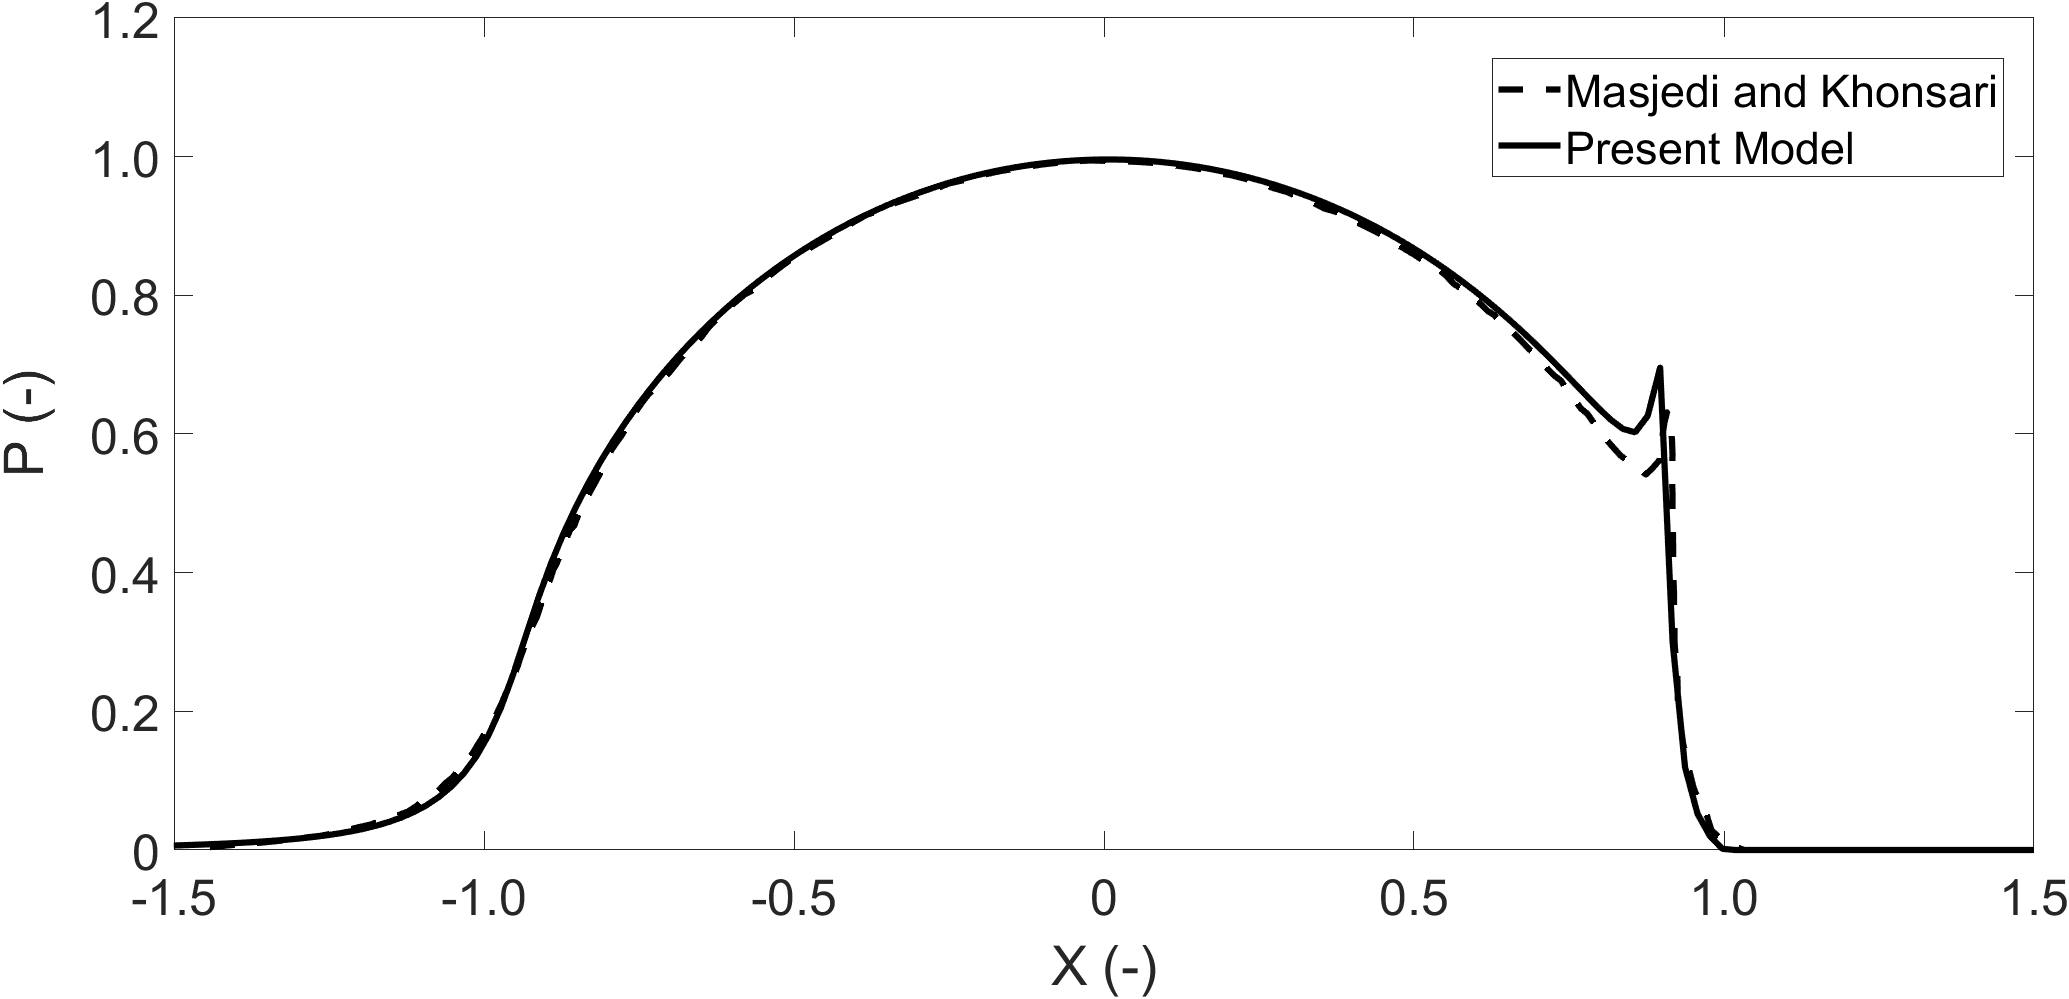
\includegraphics[width=120 mm]{ExpTribo Figure 9 - Validation of dimensionless pressure distribution, present model (solid), Masjedi and Khonsari (dashed).png}}
	\caption{Validation of dimensionless pressure distribution, present model (solid), Masjedi and Khonsari (dashed).}
	\label{EHL Pressure Validation Masjedi Khonsari}
\end{figure}

\begin{figure}
	\centerline{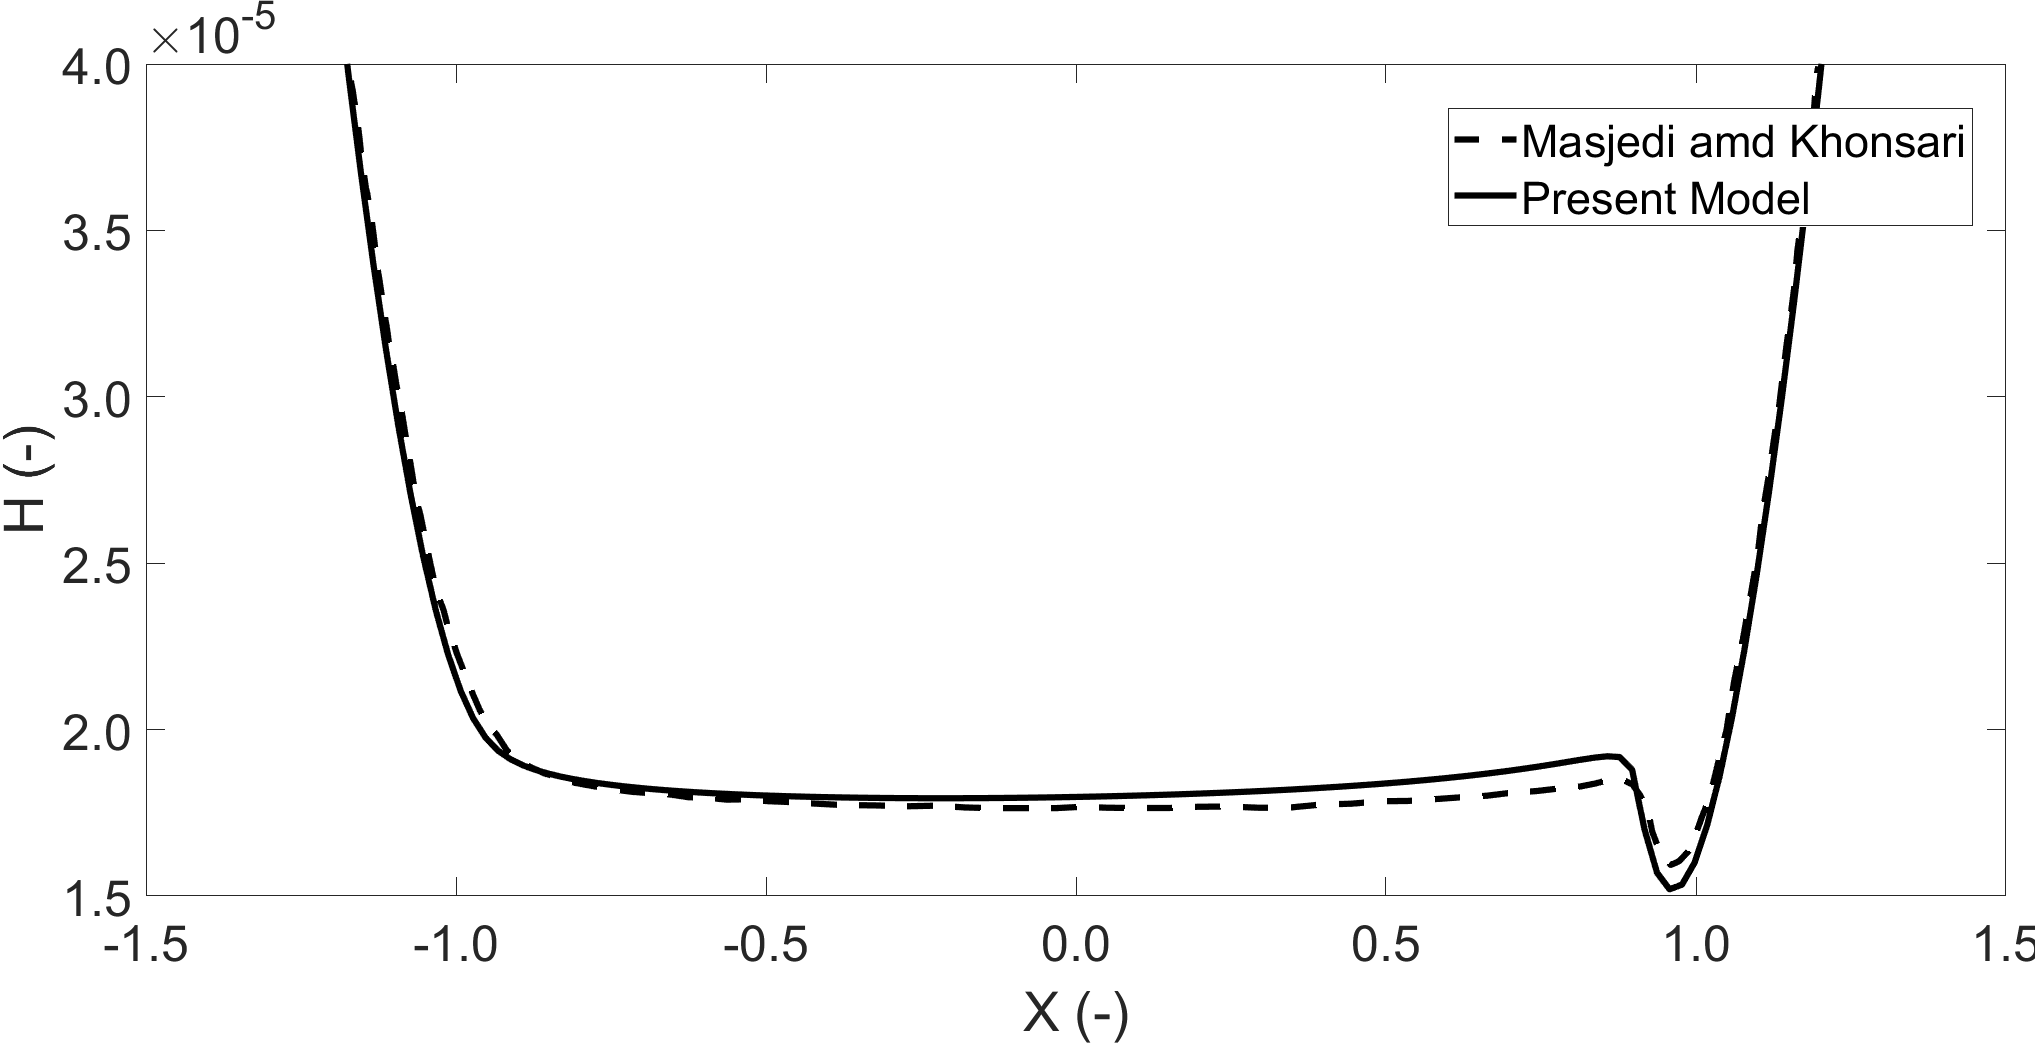
\includegraphics[width=120 mm]{ExpTribo Figure 10 - Validation of dimensionless film thickness distribution, present model (solid), Masjedi and Khonsari (dashed).png}}
	\caption{Validation of dimensionless film thickness distribution, present model (solid), Masjedi and Khonsari (dashed)}
	\label{EHL Film Validation Masjedi Khonsari}
\end{figure}

\subsection{Experimental Result Verification}
The experimental results obtained from the presented rig were verified against analytically calculated frequency contents. This was to ensure the correct post processing of data for the input to numerical models. The bearing and lubricant data properties are given in Table \ref{Bearing Specification} and Table \ref{Lubricant and Material Properties} respectively which were also used in simulations.

\begin{table*}
	%\captionsetup{justification=centering}
	\caption{Bearing Specification}
	\label{Bearing Specification}
	\centering
	\renewcommand{\arraystretch}{1.5}%
	\begin{tabular}{|c|c|}
		\hline
		\ \textbf{Parameter} & \textbf{Value} \\ [0.5ex]
		\hline
		Inner Race Bore & 25 $mm$ \\ [0.5ex]
		\hline
		Inner Race Diameter & 31.5 $mm$ \\ [0.5ex]
		\hline
		Outer Race Diameter & 46.5 $mm$ \\ [0.5ex]
		\hline
		Roller Diameter & 7.5 $mm$ \\ [0.5ex]
		\hline
		Roller Length & 9 $mm$ \\ [0.5ex]
		\hline
		Number of Rollers & 12 \\ [0.5ex]
		\hline
		External Load & 740 $N$ \\ [0.5ex]
		\hline
		Radial Interference & 0 $\mu m$ \\ [0.5ex]
		\hline
	\end{tabular}
\end{table*}

\begin{table*}
	%\captionsetup{justification=centering}
	\caption{Lubricant and Material Properties}
	\label{Lubricant and Material Properties}
	\centering
	\renewcommand{\arraystretch}{1.5}%
	\begin{tabular}{|c|c|}
		\hline
		\ \textbf{Parameter} & \textbf{Value} \\ [0.5ex]
		\hline
		Pressure Viscosity Coefficient ($\alpha$) & 2.1 $\times 10^{-8}\mathrm{~Pa}^{-1}$ \\ [0.5ex]
		\hline
		Atmospheric lubricant dynamic viscosity & 0.08 Pa.s \\ [0.5ex]
		\hline
		Lubricant inlet density ($\rho_0$) & 833.8 $\mathrm{~kg}\cdot\mathrm{m}^{-3}$ \\ [0.5ex]
		\hline
		Eyring stress ($\tau_0$) & 2 $MPa$ \\ [0.5ex]
		\hline
		Shear strength of asperities ($\varsigma$) & 0.3 \\ [0.5ex]
		\hline
		Thermal conductivity of fluid & 1600 $\mathrm{~W}\cdot\mathrm{m}^{-1}\cdot\mathrm{K}^{-1}$ \\ [0.5ex]
		\hline
		Modulus of elasticity of contacting solids & 210 GPa \\ [0.5ex]
		\hline
		Poisson’s ratio of contacting solids & 0.3 \\ [0.5ex]
		\hline
        Density of contacting solids & 7850 $\mathrm{~kg}\cdot\mathrm{m}^{-3}$ \\ [0.5ex]
		\hline
		Thermal conductivity of contacting solids & 46 $\mathrm{~W}\cdot\mathrm{m}^{-1}\cdot\mathrm{K}^{-1}$ \\ [0.5ex]
		\hline
		Specific heat capacity of contacting solids & 470 $\mathrm{~J}\cdot\mathrm{kg}^{-1}\cdot\mathrm{K}^{-1}$ \\ [0.5ex]
		\hline
	\end{tabular}
\end{table*}

Primary frequencies in the system due to the interaction of the rolling elements, races and the shaft could then be verified. These frequencies were calculated analytically, with $f_{bpi}$ and $f_{bpo}$ representing the ball pass frequencies of the inner and outer race respectively and $f_{shaft}$ being the rotational frequency of the shaft:

\begin{equation}\label{ball pass frequency inner}
	f_{b p i}=\frac{\omega_s}{2 \pi} \frac{N}{2}\left(1-\frac{D_r}{D_p}\right)
\end{equation}

\begin{equation}\label{ball pass frequency outer}
	f_{b p o}=\frac{\omega_s}{2 \pi} \frac{N}{2}\left(1+\frac{D_r}{D_p}\right)
\end{equation}

\begin{equation}\label{ball pass frequency shaft}
	f_{\text {shaft }}=\frac{\omega_s}{2 \pi}
\end{equation}

At 14~000~$rpm$, the theoretical inner and outer race frequencies are calculated to be 1669~$Hz$ and 1131~$Hz$ respectively, with the experimental results being 1611~$Hz$ and 1131~$Hz$. The first order shaft rotational frequency from the experiment was 232~$Hz$ compared to theoretical calculation of 233~$Hz$. The above frequencies can be seen clearly in Figure 7, which shows the bearing bore displacement spectra, and Figure 8 which represents the shaft displacement spectra. The verification frequencies are identical in both, confirming that the bearing motion is accurately measured by the experimental methodology. It is observed that at certain speeds, the ball pass frequency of the outer race has a larger contribution than the inner race. This is particularly highlighted at 12~000~-~14~000~$rpm$. These regional effects are contributed by modal behaviour of the bracket and the bed. The critical speed of the unloaded shaft, where lateral bending frequency of the shaft is equal to the rotation frequency \cite{Shigley'sMechanicalEngineeringDesign}, occurs at 12~660~$rpm$ and 211~$Hz$.

\begin{figure}
	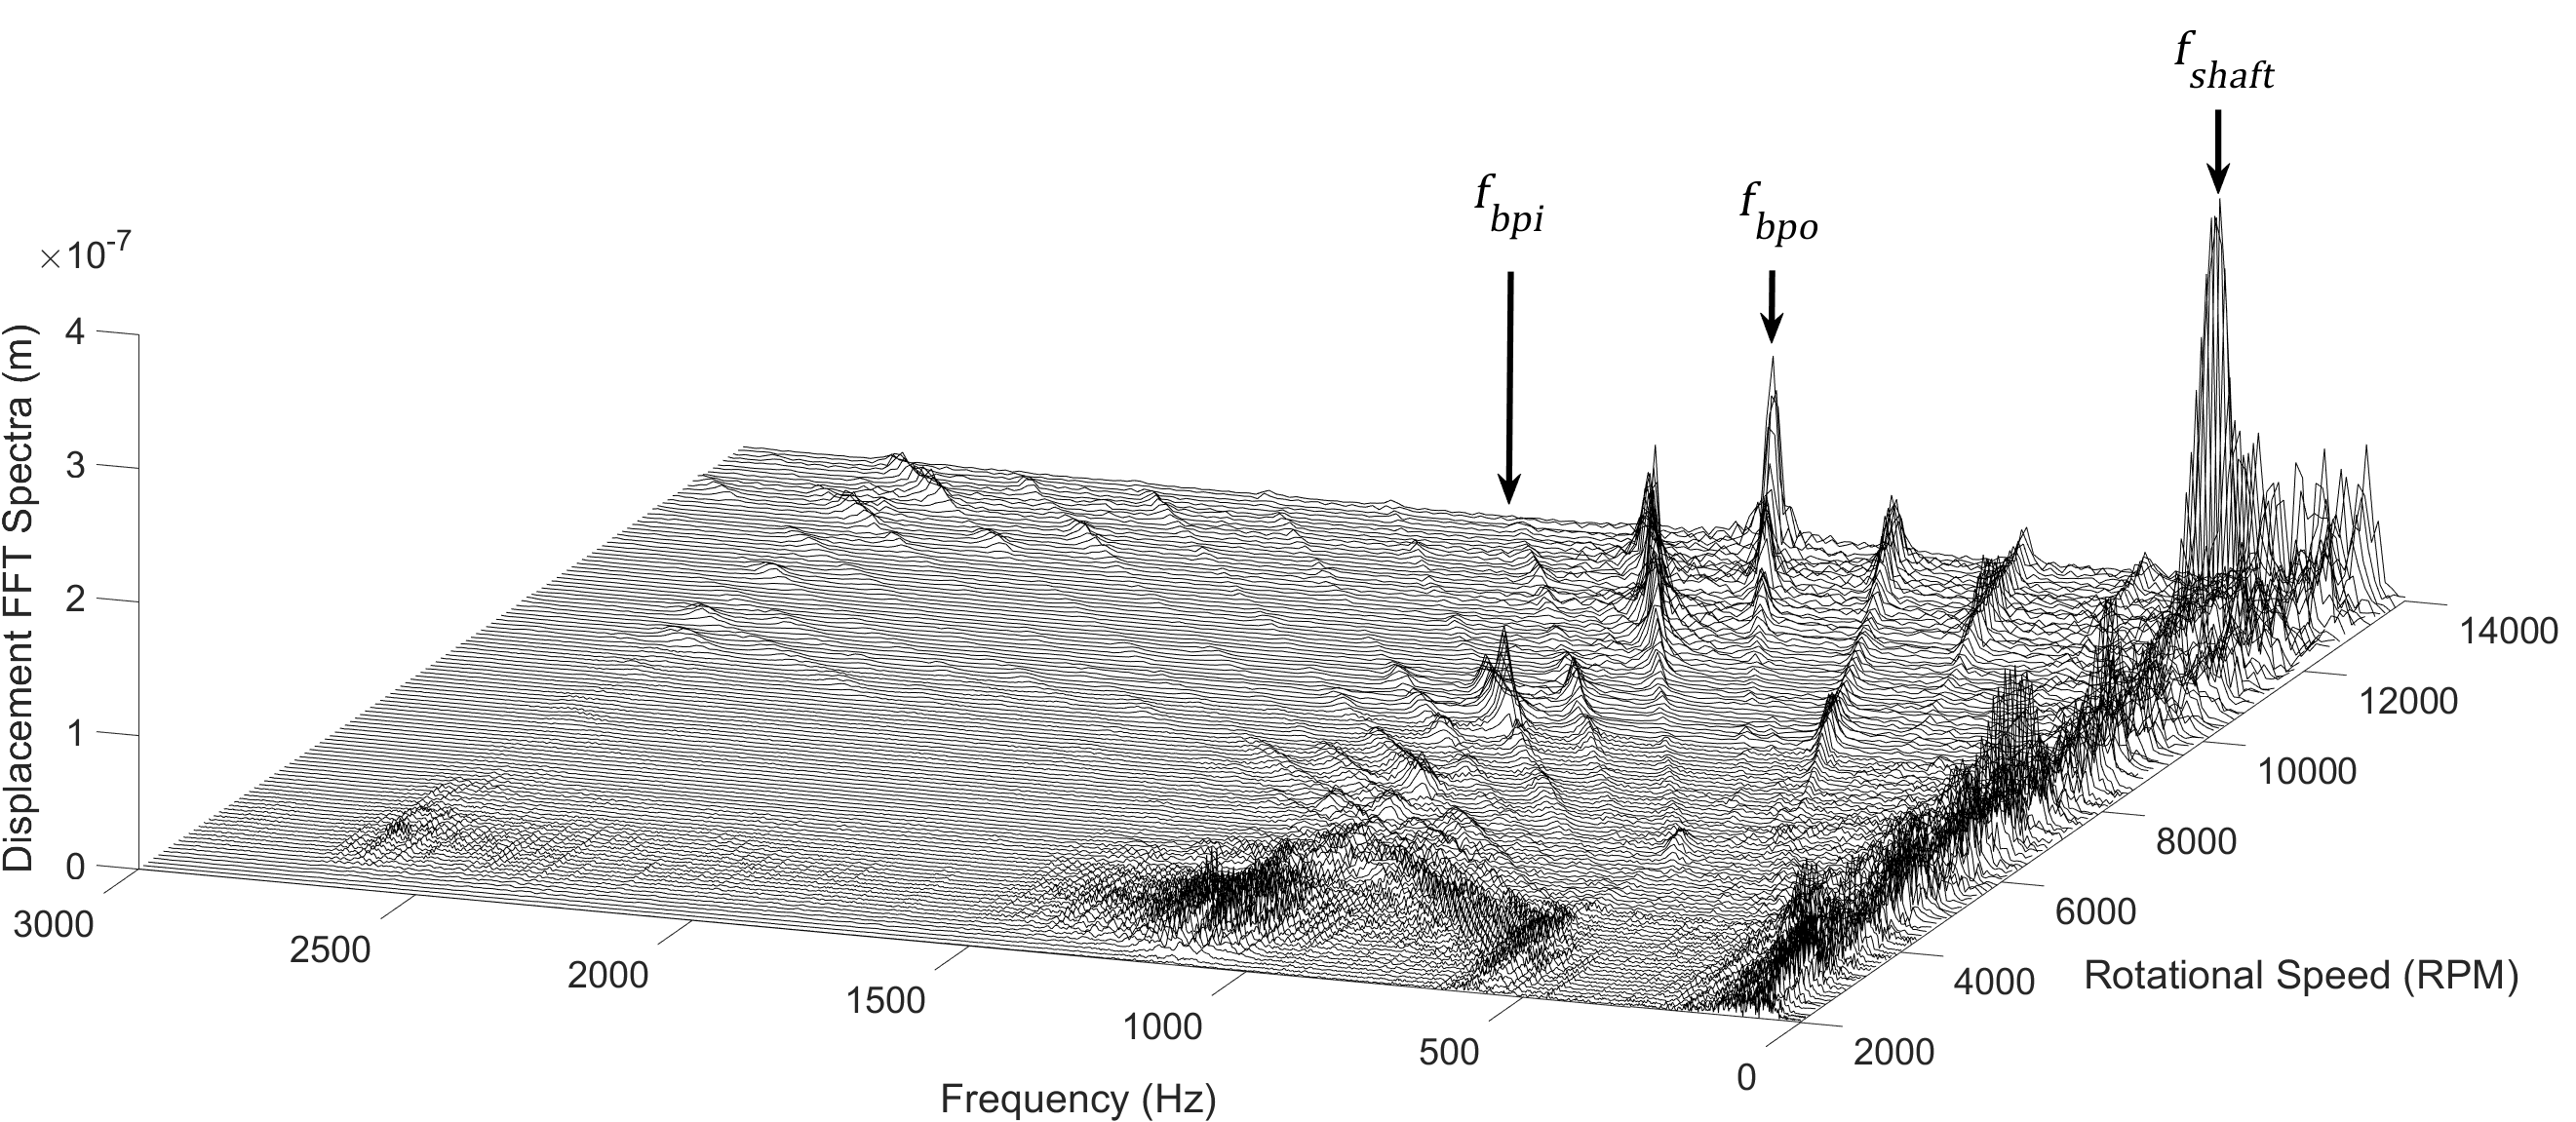
\includegraphics[width=150mm]{ExpTribo Figure 7 - Bearing Bore Displacement Frequency Spectra.png}
	\caption{Bearing bore displacement frequency spectra.}
	\label{Bearing bore displacement frequency spectra}
\end{figure}

\begin{figure}
	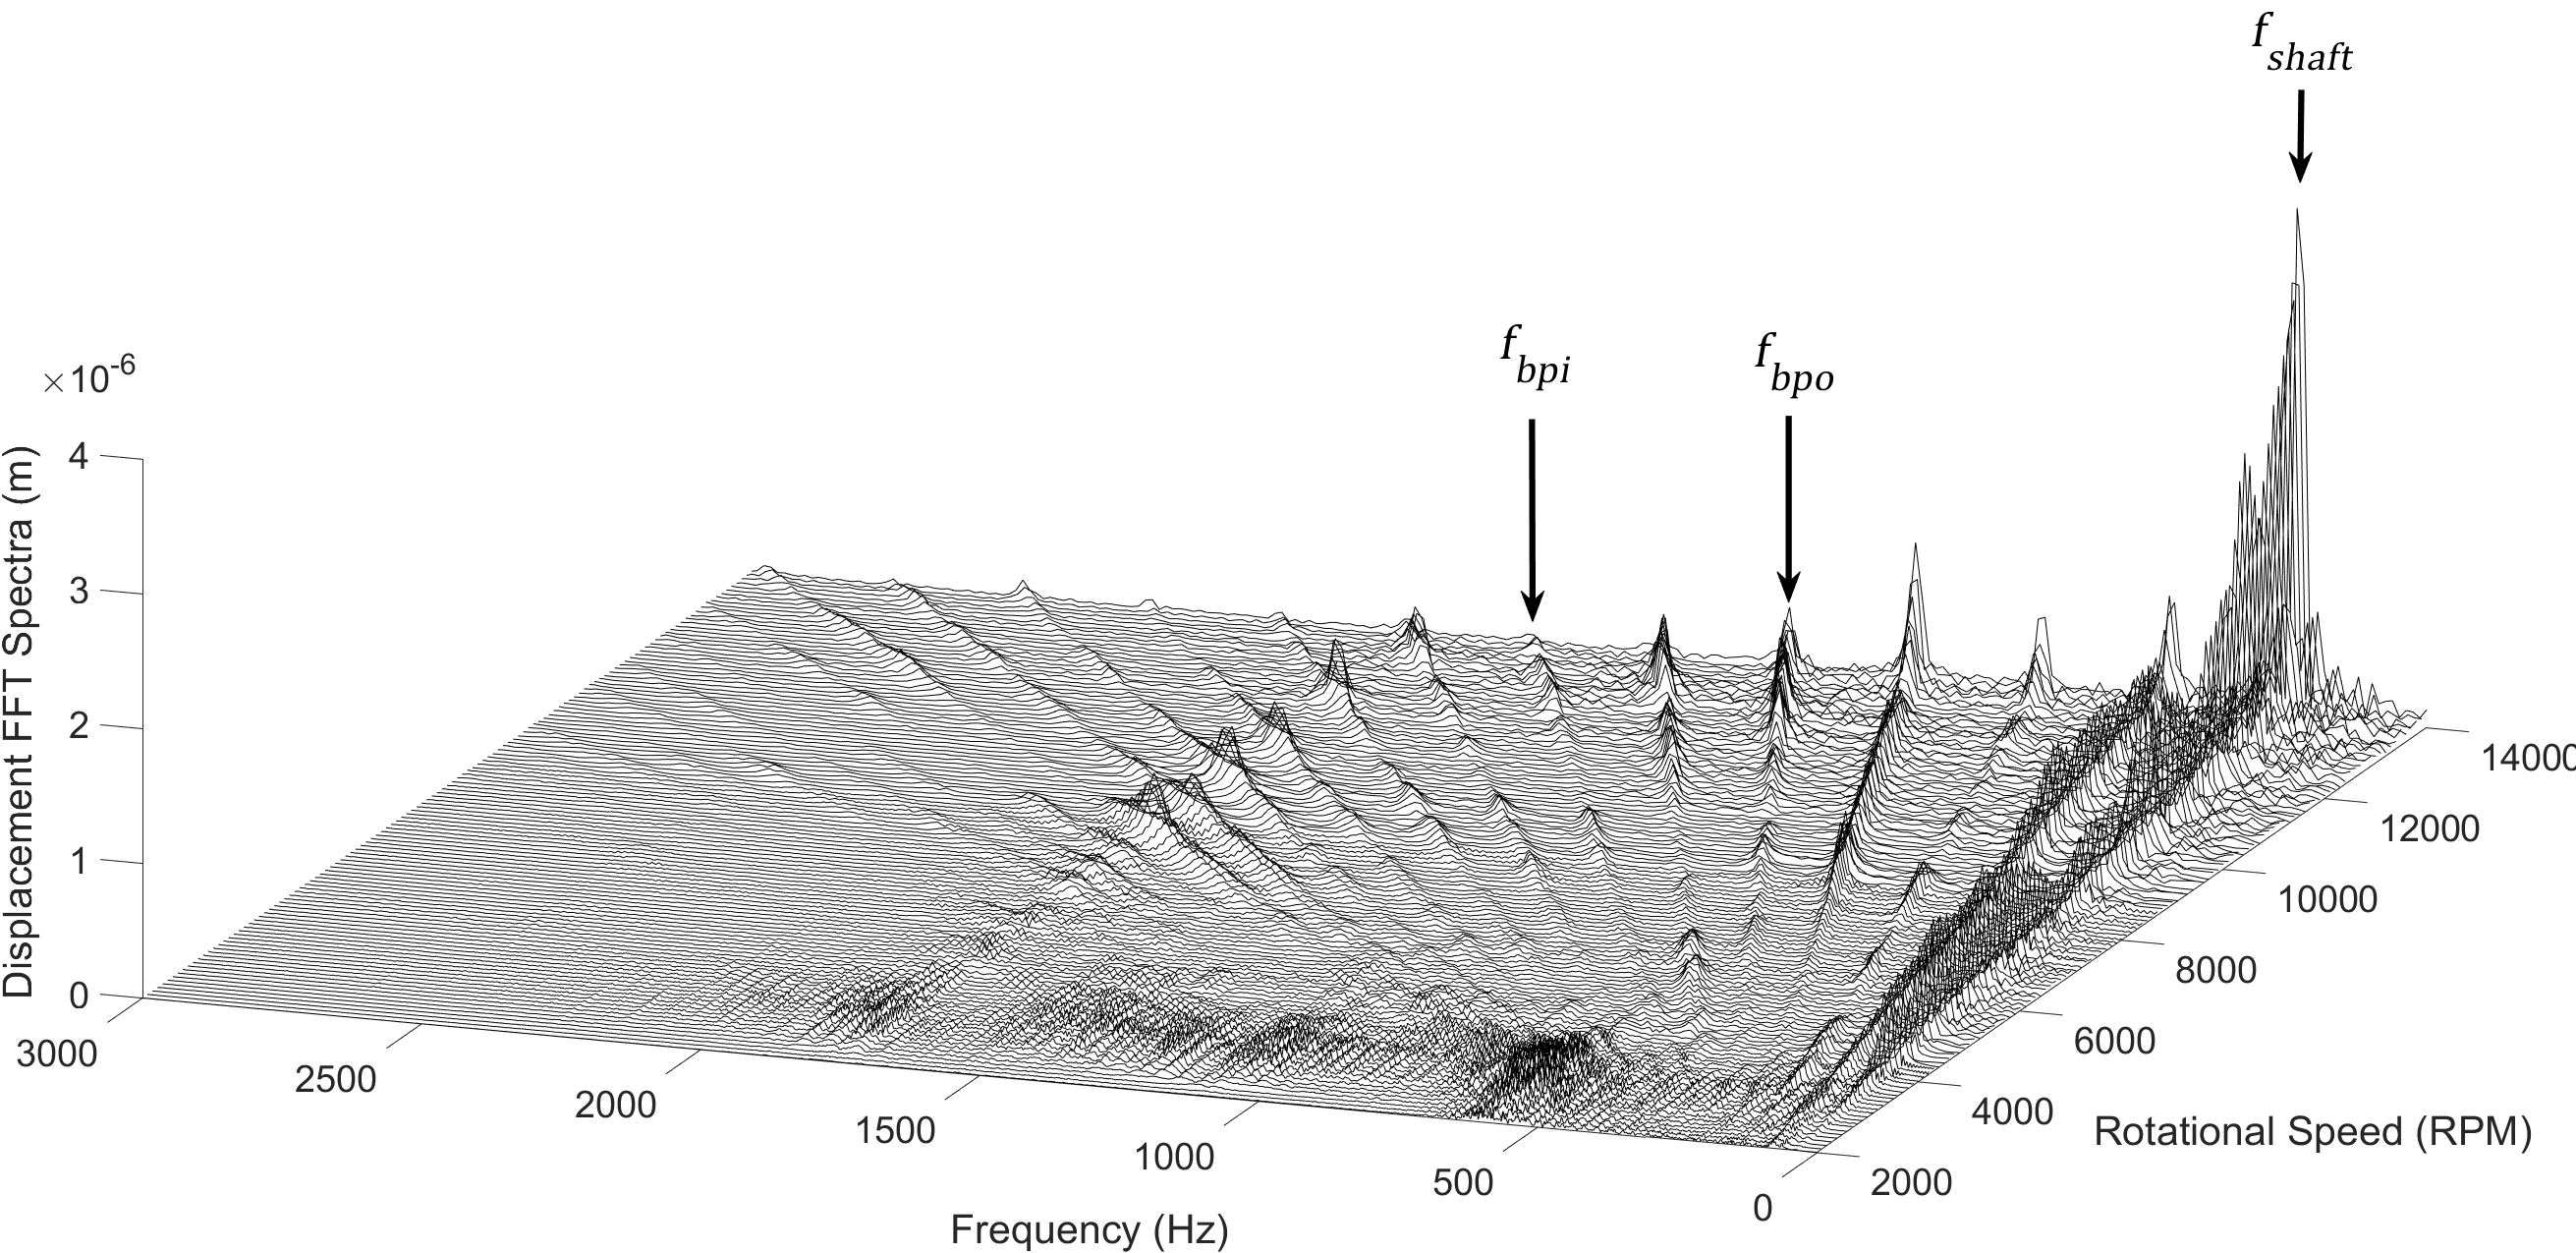
\includegraphics[width=150mm]{ExpTribo Figure 8 - Shaft Displacement Frequency Spectra.png}
	\caption{Shaft displacement frequency spectra.}
	\label{Shaft displacement frequency spectra}
\end{figure}

\section{Results and Discussion}
This section presents the results of the numerical tribological models. The kinematic data from the experimental test rig are used as the boundary conditions to the implicit and explicit models.

\subsection{Film thickness and load across speed sweep} 
The variation in EHL film thickness and roller contact load across the speed sweep from 0~-~15~000~$rpm$ at the outer race contact are shown in Figure \ref{Contact load and film thickness - Outer race}. Only the EHL regions are shown, where loads are significant enough to cause contact deformation. The upper limit of the film is where the roller and races diverge and approach the hydrodynamic regime where the film is hence governed by the entraining motion of lubricant into the contact. The lubricant film, as seen from the film thickness equation, is more affected by the speed of entraining motion rather than the load. This explains the increasing film thickness values in Figure \ref{Contact load and film thickness - Outer race} despite increasing load. The film thickness is increased from 0.1 to 1.9~$\mu m$ across the speed sweep, revealing a significant increase that can affect the tribodynamic behaviour of the bearing, as explained in following sections. From the tribological model, it is possible to observe the transition between mixed-EHL to the purely hydrodynamic regime as the roller passes in and out of the loaded region of the bearing. Full system and rotor dynamics also contribute to the total load on the roller, with periods of resonance at 3~000~$rpm$ and 14~000~$rpm$ marked as $A$ and $B$ respectively in Figure \ref{Contact load and film thickness - Outer race}.

\begin{figure}
	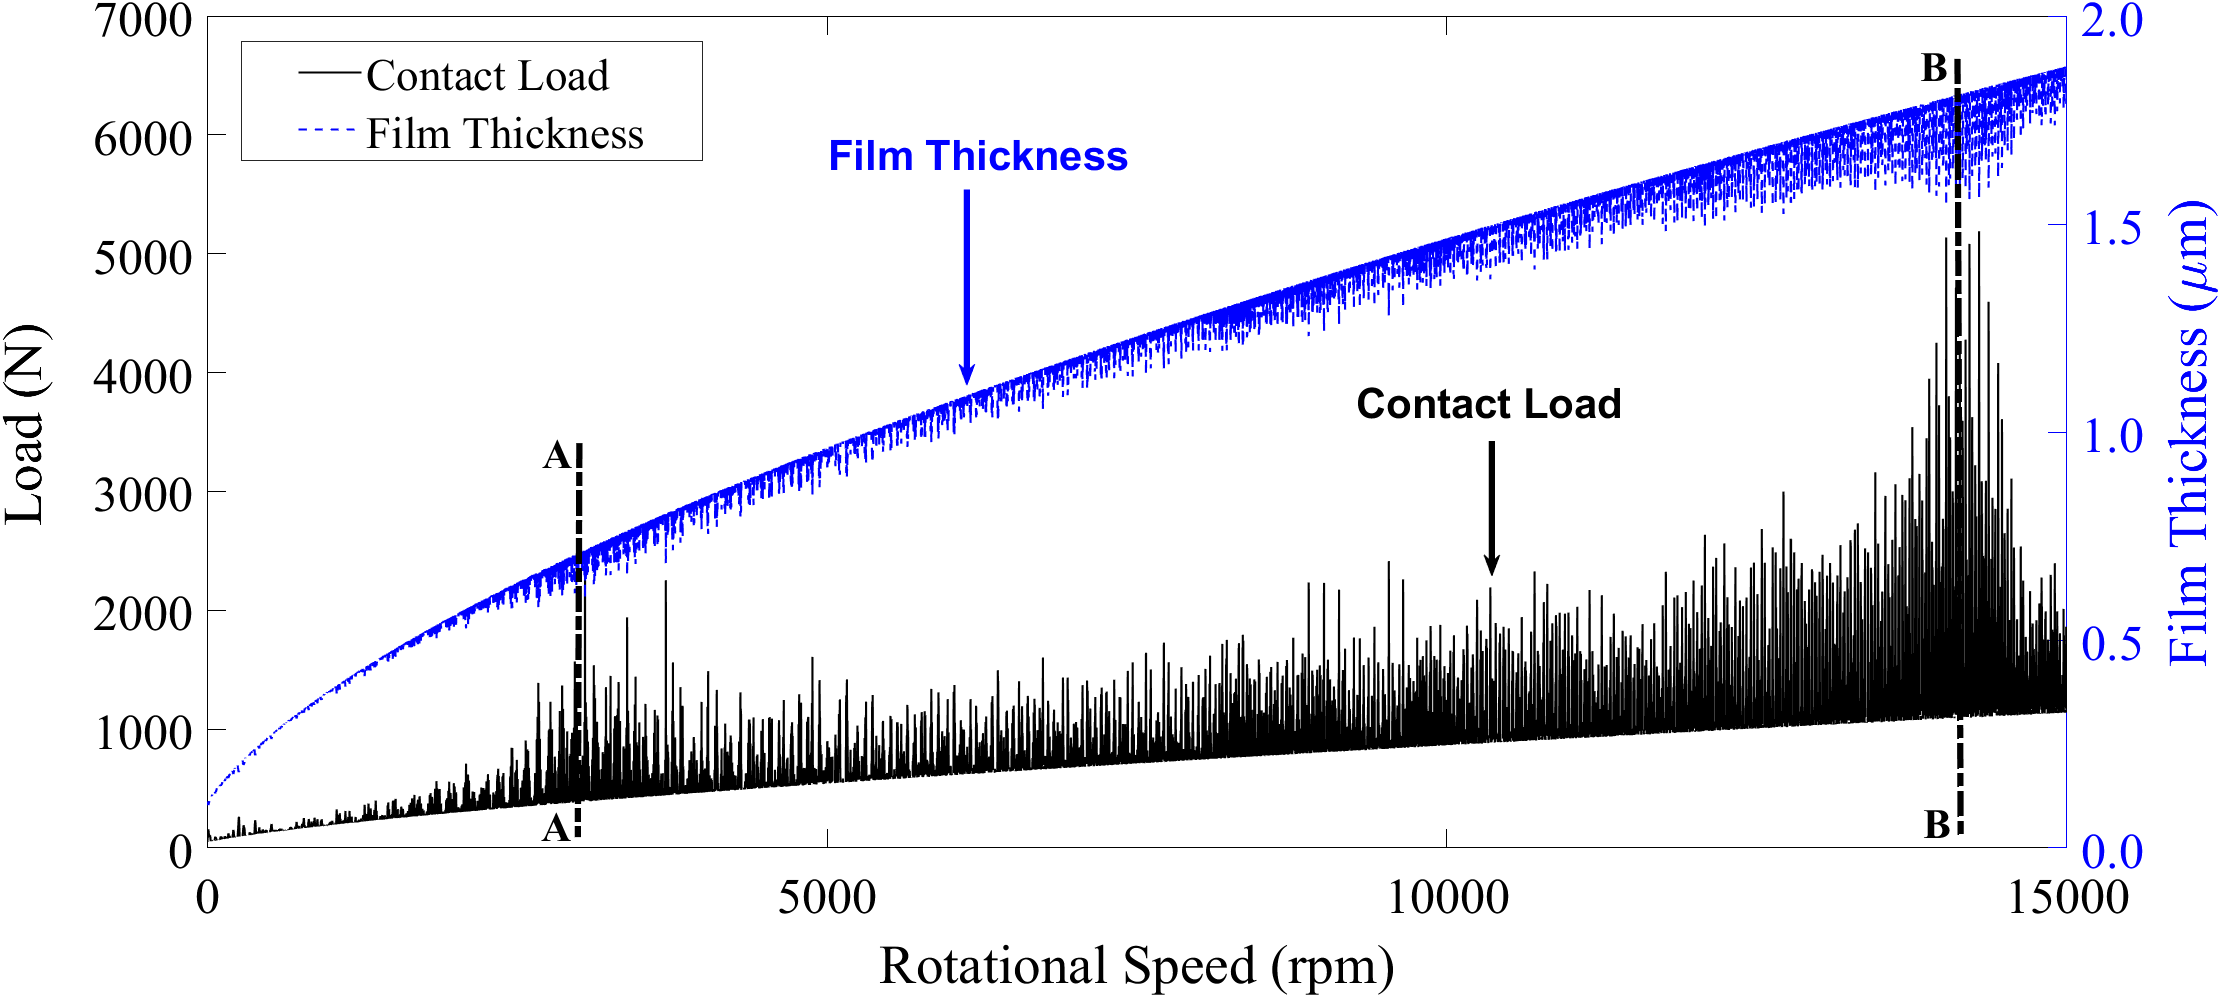
\includegraphics[width=150mm]{ExpTribo Figure 11 - Contact Load and Film Thickness - Outer Race.png}
	\caption{Contact load and film thickness - Outer race.}
	\label{Contact load and film thickness - Outer race}
\end{figure}

Figure \ref{Film and load - EHL to hydrodynamic regime} presents an interval of the speed sweep where the effect of the EHL load on reducing the film thickness under oscillating conditions can be observed and the hydrodynamic film growth as the roller is unloaded. It is possible to see the effect of the resonant frequency at 1765~$Hz$ superimposed on the lower fundamental train frequency within the loaded region as the inner and outer rings converge and diverge. The results in Figure \ref{Film and load - EHL to hydrodynamic regime} confirm the significant effect of dynamic behaviour as well as multi-regime nature of the lubrication due to dynamic effects.

\begin{figure}
	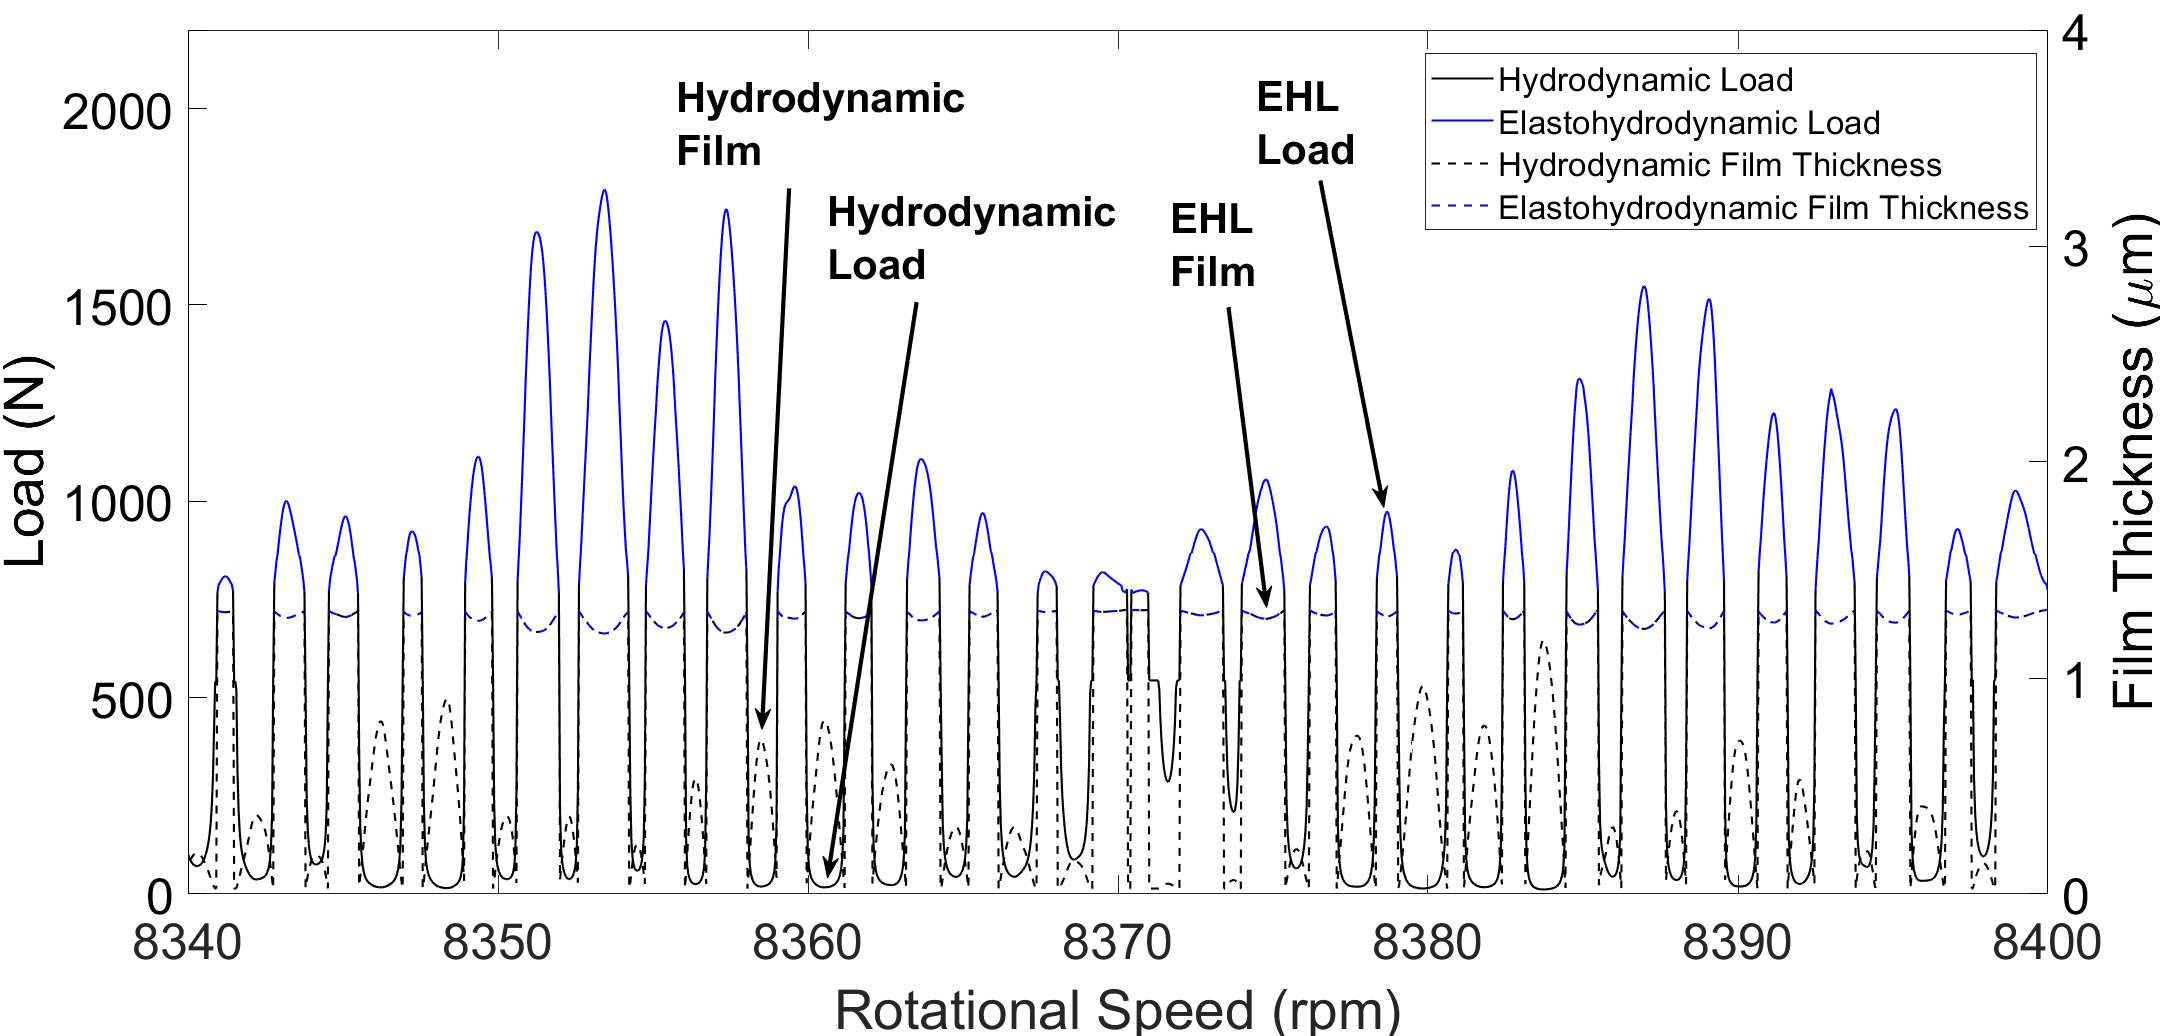
\includegraphics[width=150mm]{ExpTribo Figure 12 - Film and Load - EHL to Hydrodynamic Regime.png}
	\caption{Film and load - EHL to hydrodynamic regime.}
	\label{Film and load - EHL to hydrodynamic regime}
\end{figure} 

\subsection{Friction} 
Focussing on data from the EHL regime, boundary and viscous friction through the speed sweep can be analysed. Figure \ref{Viscous and boundary friction at the outer race contact} shows the boundary and viscous friction across the speed sweep. As the film thickness increases with speed, the separation of the contacting surfaces increases, reducing the boundary interaction of asperities. The resonant period at 14~000~$rpm$ reduces the film height, increasing the likelihood of asperity interaction in that region and hence boundary friction and potential for wear. In general, the boundary friction reduces towards higher rotational and entrainment velocities. This does not, however, account for lubricant inlet starvation at high speeds or roller sliding. Viscous friction increases with higher speed and hence the shear as expected. Although the film thickness also increases at higher speeds which may reduce the amount of shear, the effect of increasing speed is more dominant. The peak values occurring again at a resonance speed of 14~000~$rpm$ where the highest loads and smallest film occurs. 

\begin{figure}
	\includegraphics[width=150mm]{ExpTribo Figure 13 – Viscous and Boundary Friction at Outer Race Contact.png}
	\caption{Viscous and boundary friction at the outer race contact.}
	\label{Viscous and boundary friction at the outer race contact}
\end{figure} 

\subsection{EHL Regimes} 

As has been demonstrated in the results analysis, the contact conditions deviate from the elastohydrodynamic regime of lubrication into the hydrodynamic regime throughout the roller orbital motion. These conditions can be verified by presenting the results on the Greenwood chart for fluid regimes of lubrication. The charts display the physical effects instrumental to EHL formation under isothermal conditions: viscosity rise due to pressure and elastic deformation of the surface. These two effects are quantified by two dimensionless parameters, $G_e$ and $G_v$, as defined below \cite{Gohar1988}: 

\begin{equation}\label{GoharGe}
	G_e=\frac{W^*}{U^{* 1 / 2}}
\end{equation}

\begin{equation}\label{GoharGv}
	G_v=\frac{W^{* 3 / 2} G^*}{U^{* 1 / 2}}
\end{equation}

Four regions exist and the boundaries of these regions are defined by the geometry of contacting bodies, material, and lubricant properties. As is shown in Figure \ref{EHL and hydrodynamic conditions during roller operation}, the outer roller-race contact conditions move between the viscous elastic and iso-viscous rigid regimes, representing EHL and hydrodynamic respectively. The viscous elastic regime signifies the EHL regime of lubrication where contact pressures are such that elastic deformation of the surfaces and viscosity rise due to pressure increase is significant. The iso-viscous rigid regime occurs when the magnitude of elastic deformation is insignificant, and the contact pressures are low enough that viscosity rise is negligible, i.e. hydrodynamic lubrication \cite{Hamrock1980}. The boundary between the two also corresponds well with the distinction being made between hydrodynamic and EHL in this methodology, presented by the black and blue regions of the plot.

\begin{figure}
	\includegraphics[width=150mm]{ExpTribo Figure 14 – EHL and hydrodynamic conditions during roller operation.png}
	\caption{EHL and hydrodynamic conditions during roller operation. Key: IR = Iso-viscous Rigid, VR = Viscous Rigid, VE = Viscous Elastic, IE = Iso-viscous Elastic.}
	\label{EHL and hydrodynamic conditions during roller operation}
\end{figure} 

\subsection{Dry vs Lubricated Tribodynamic Model}

Previously presented results confirmed the significance of considering tribodynamic coupling on the tribological predictions. The aim of this section is to assess the significance of this coupling on dynamics via affecting contact load and stiffness values. The surface deformation at the EHL contact is further exacerbated by the presence of the lubricant film. Since the contact load and contact stiffness are governed by this deformation, neglecting the film leads to an underestimation of the total load at the roller-race contact. At higher speeds, such as those present in modern electrified powertrains, the growth of the lubricant film due to the increased entraining motion into the conjunction cannot be neglected – as is shown in Figure \ref{Contact load and film thickness - Outer race} with a film growth from 0.1 to 1.9~$\mu m$. The implicit tribological model was run for two cases, including and negating lubricant film thickness in the deformation obtained from Equation \ref{Contact deflection experimental}. The difference in magnitude at each time step is computed, and the increase in load magnitude between a dry and lubricated model is calculated. For EHL loads, the magnitude of the load difference through the speed sweep is plotted in Figure \ref{Contact load difference between dry and lubricated model}.

\begin{figure}
	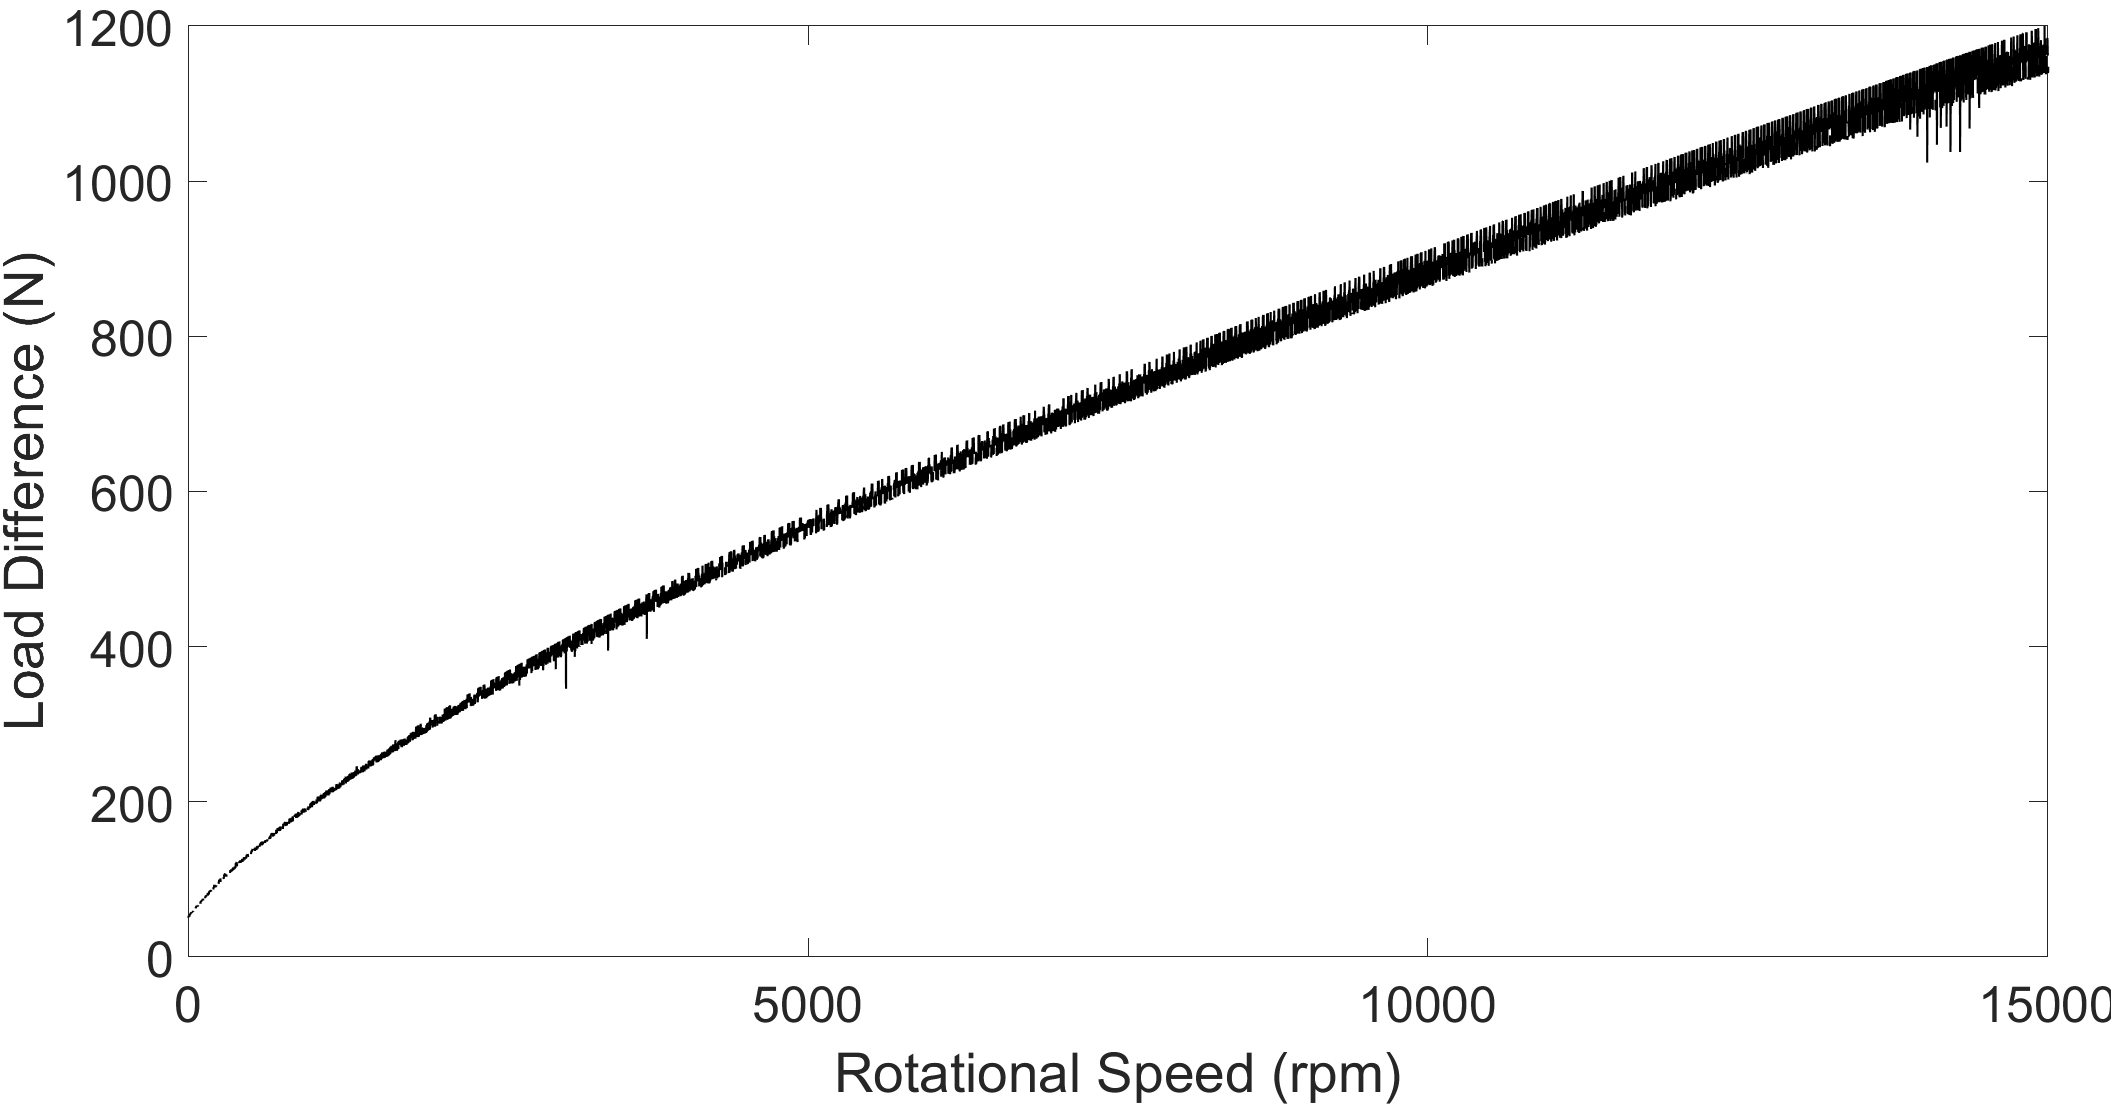
\includegraphics[width=150mm]{ExpTribo Figure 15 - Contact Load Difference Between Dry and Lubricated Model.png}
	\caption{Contact load difference between dry and lubricated model.}
	\label{Contact load difference between dry and lubricated model}
\end{figure} 

There is an increasing load difference across the speed sweep, with fluctuations arising from the dynamics of the system. It is clear that neglecting lubricant film thickness leads to significant underestimation of the contact load, hence inaccurate dynamics as well as tribological calculations. This effect gains more significance at higher speeds which highlights the necessity of considering tribodynamic coupling for high-speed conditions in electrified powertrains. To fully understand the requirement for a lubricated bearing model, the percentage difference between both cases is presented at three different rotational speed snapshots of 3~050~$rpm$, 14~135~$rpm$, and 14~855~$rpm$ in Figure \ref{Dry and lubricated model load difference}. At low speeds and relatively low dynamic load, the addition of the film contributes to a 14.8\% greater load prediction than a dry model, showing that the film inclusion has a significant contribution even at low rotational speeds. At shaft speeds of 14~135~$rpm$, the first order resonance in the system, as shown in the frequency plots, creates high dynamic loading. At peak load, the growth of the film is still present, however, the high contact deformation is close to the magnitude of the film growth, hence the difference between dry and lubricated model reaches 25.1\%. As the system passes through this resonant region and the overall dynamic load is reduced, the percentage load difference reaches values as high as 149\% as the effect of the film growth at high speeds exceeds that of the surface deformation.

\begin{figure}[h!]
	\centering
	\begin{subfigure}{0.75\textwidth}
		\centering
		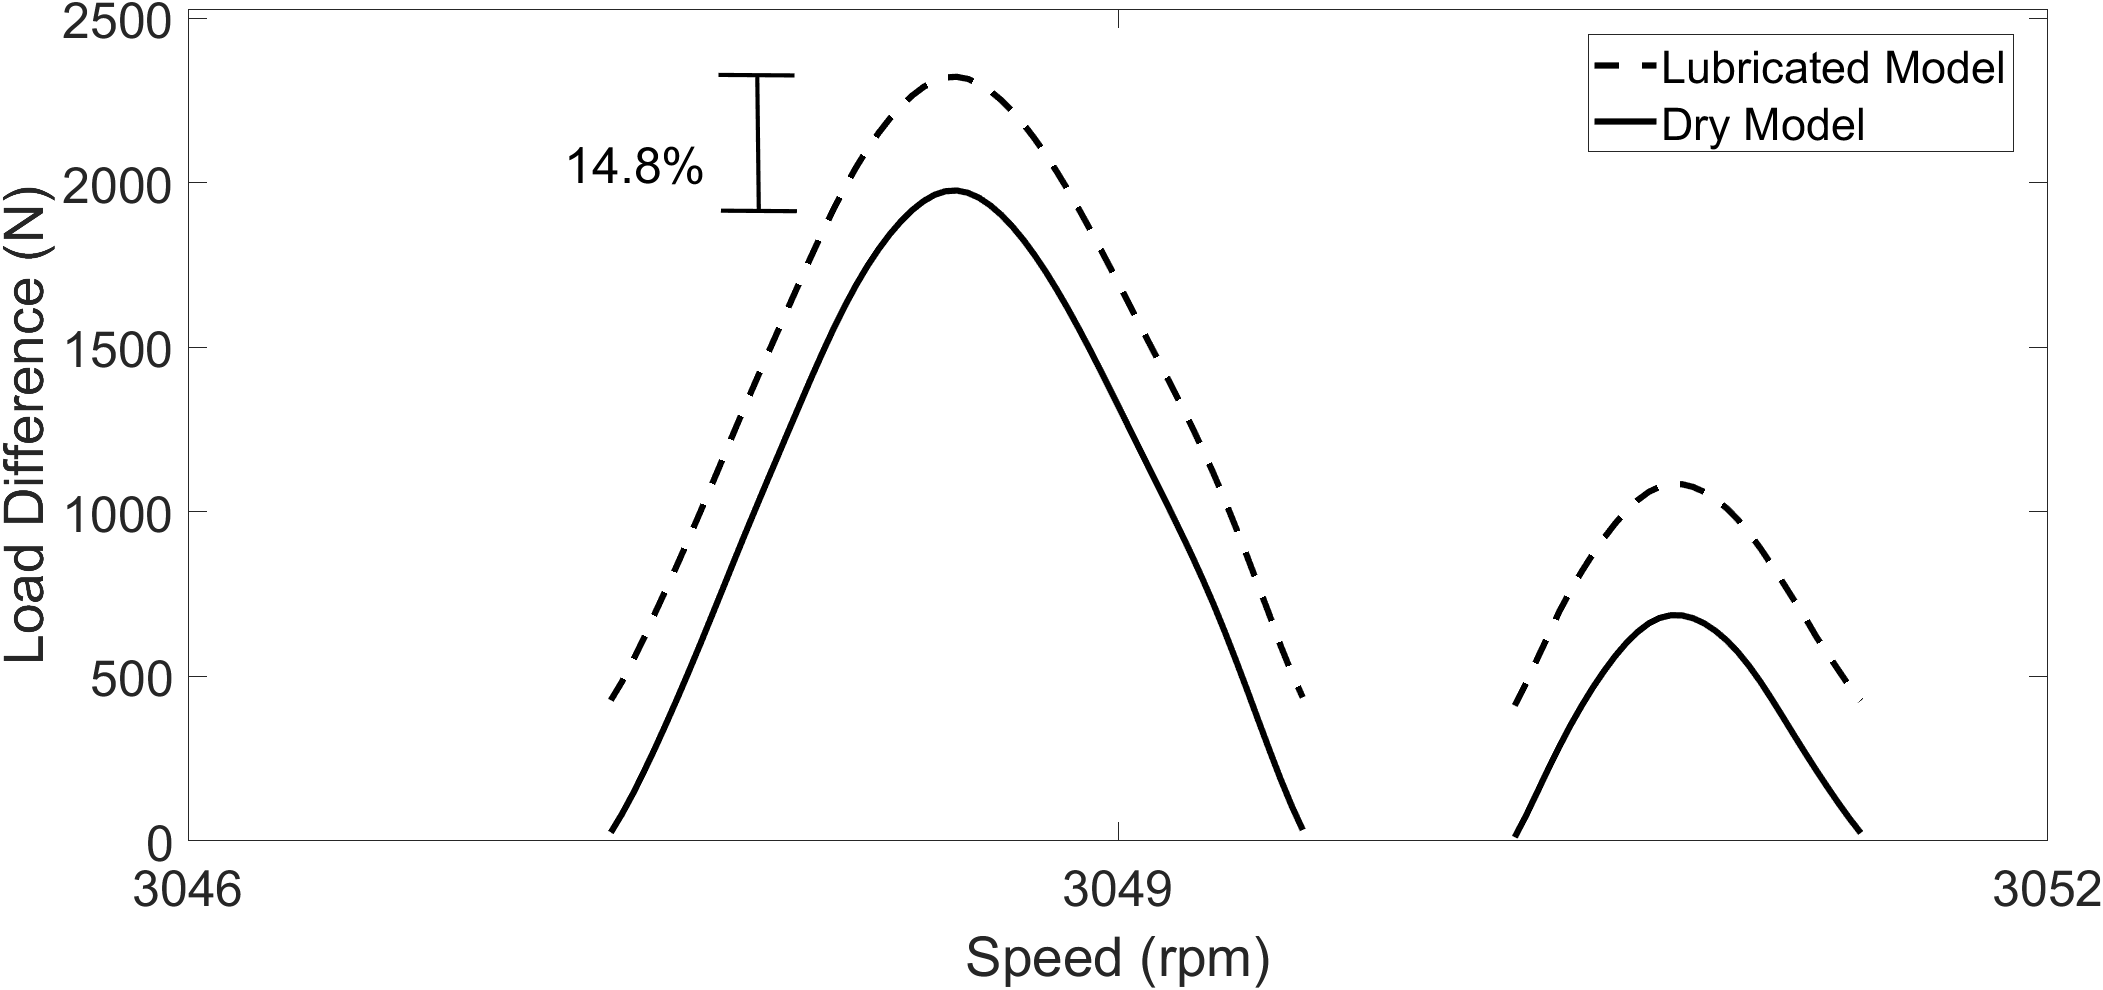
\includegraphics[width=\textwidth]{ExpTribo Figure 16a.png}
		\caption{}
		\label{3050rpm}
	\end{subfigure}
	\hfill
	\begin{subfigure}{0.75\textwidth}
		\centering
		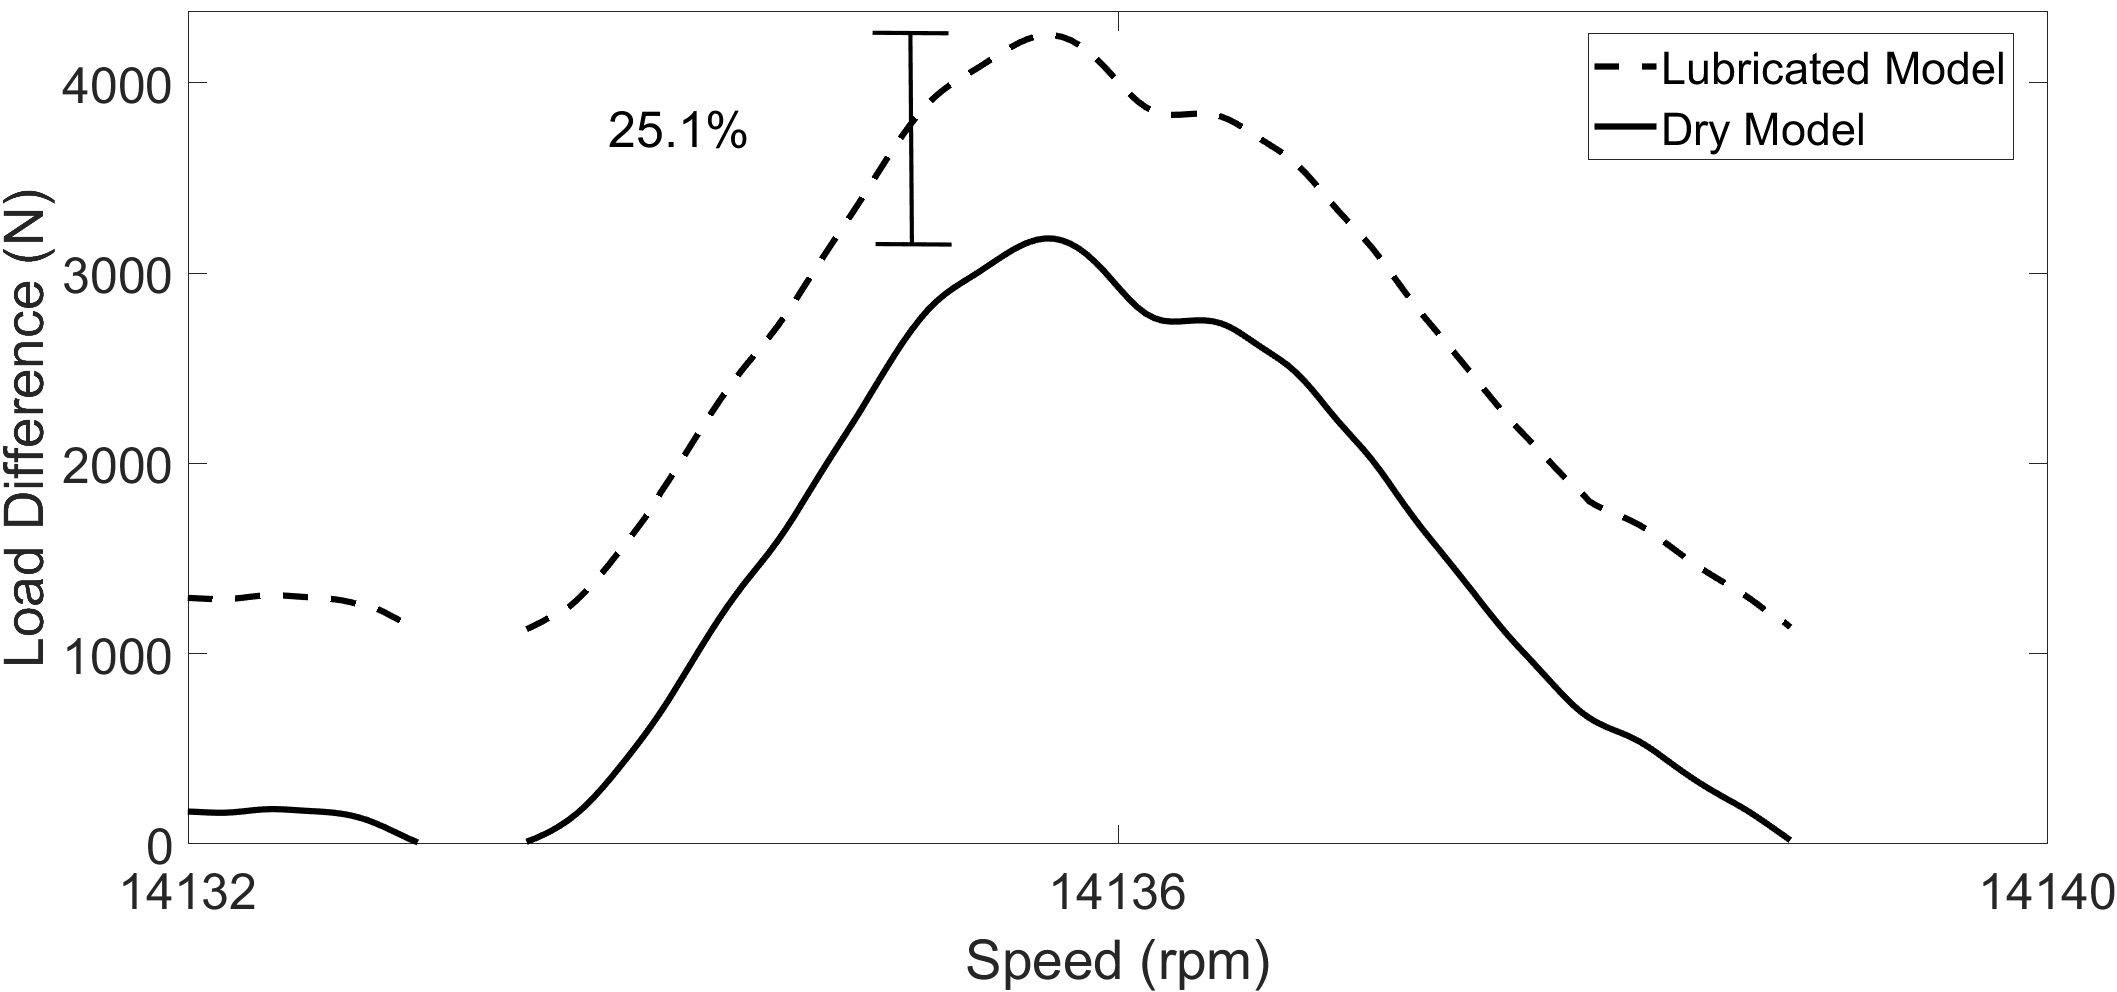
\includegraphics[width=\textwidth]{ExpTribo Figure 16b.png}
		\caption{}
		\label{14135rpm}
	\end{subfigure}
	\vfill
	\begin{subfigure}{0.75\textwidth}
		\centering
		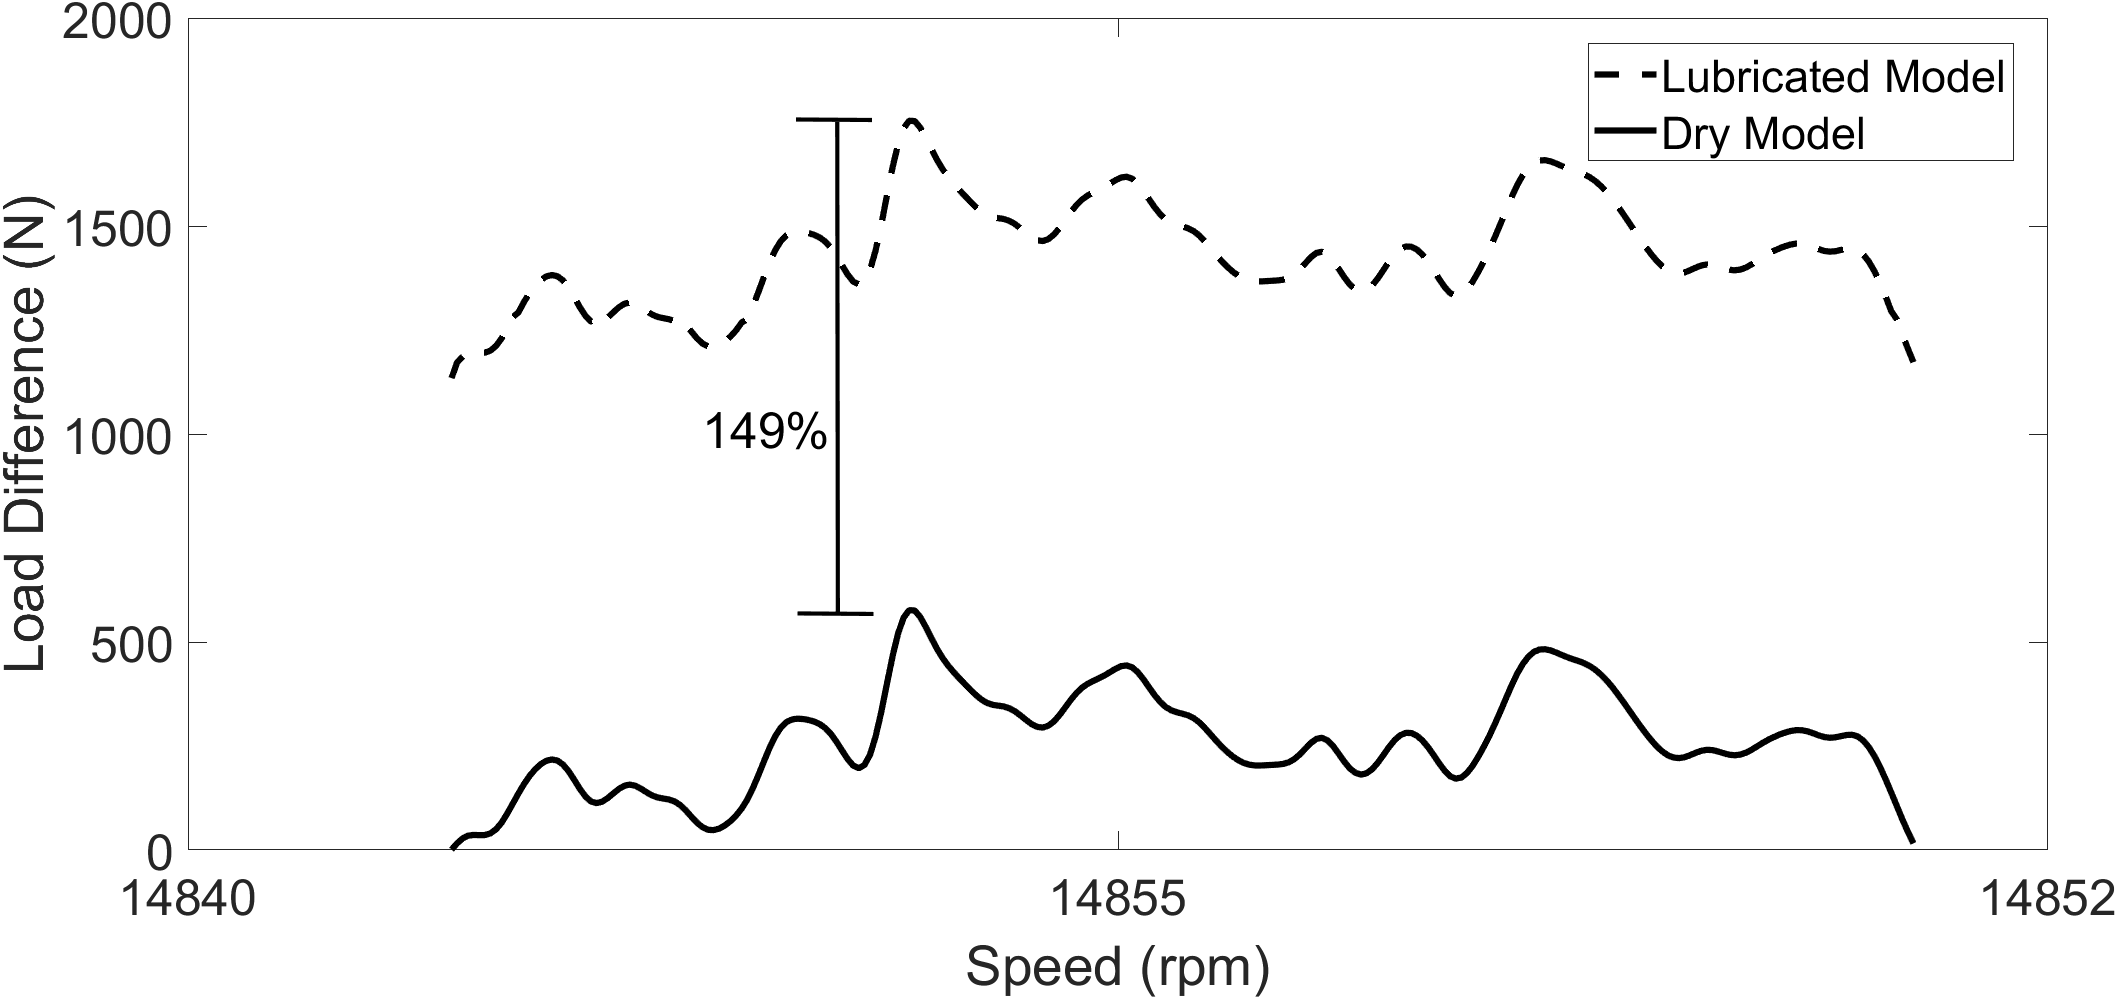
\includegraphics[width=\textwidth]{ExpTribo Figure 16c.png}
		\caption{}
		\label{14855rpm}
	\end{subfigure}
	\caption{Dry and lubricated model load difference: a) 3~050~$rpm$, b) 14~135~$rpm$, c) 14~855~$rpm$.}
	\label{Dry and lubricated model load difference}
\end{figure}

At high speeds in periods of resonance, the magnitude of the bearing load dominates, and the effect of the increasing film thickness with speed diminishes in regions of resonance. The percentage difference between the dry and lubricated model is lower as the external force and corresponding surface deformation prevails the effect of the film. However, at high speeds outside of this period of resonance, the film thickness is of the same order as the deformation and the percentage difference between the two models is much greater.  

\subsection{Numerical EHL Results}

Full numerical simulation is required to obtain detailed pressure and film thickness distributions. These distributions reveal the realistic pressure and film values at the contact for in depth durability, efficiency and thermal analysis. At 8~350~rpm, focussing on one roller orbit, the selected points for EHL numerical analysis are shown in Figure \ref{Selected points for the numerical EHL model}. These load values are found from the implicit tribological model when the roller enters the loaded region of the bearing. The corresponding points on the bearing circumference are also shown. 

\begin{figure}
	\includegraphics[width=150mm]{ExpTribo Figure 17 – Selected Points for Numerical EHL Model.png}
	\caption{Selected points for the numerical EHL model.}
	\label{Selected points for the numerical EHL model}
\end{figure} 

The load values are passed explicitly to the numerical EHL model along with entrainment velocity, lubricant and solid properties. From the nodes presented, the pressure distribution and film thickness across the contact are obtained. These are presented in Figure 18.

\begin{figure}
	\centering
	\begin{subfigure}[b]{0.49\textwidth}
		\centering
		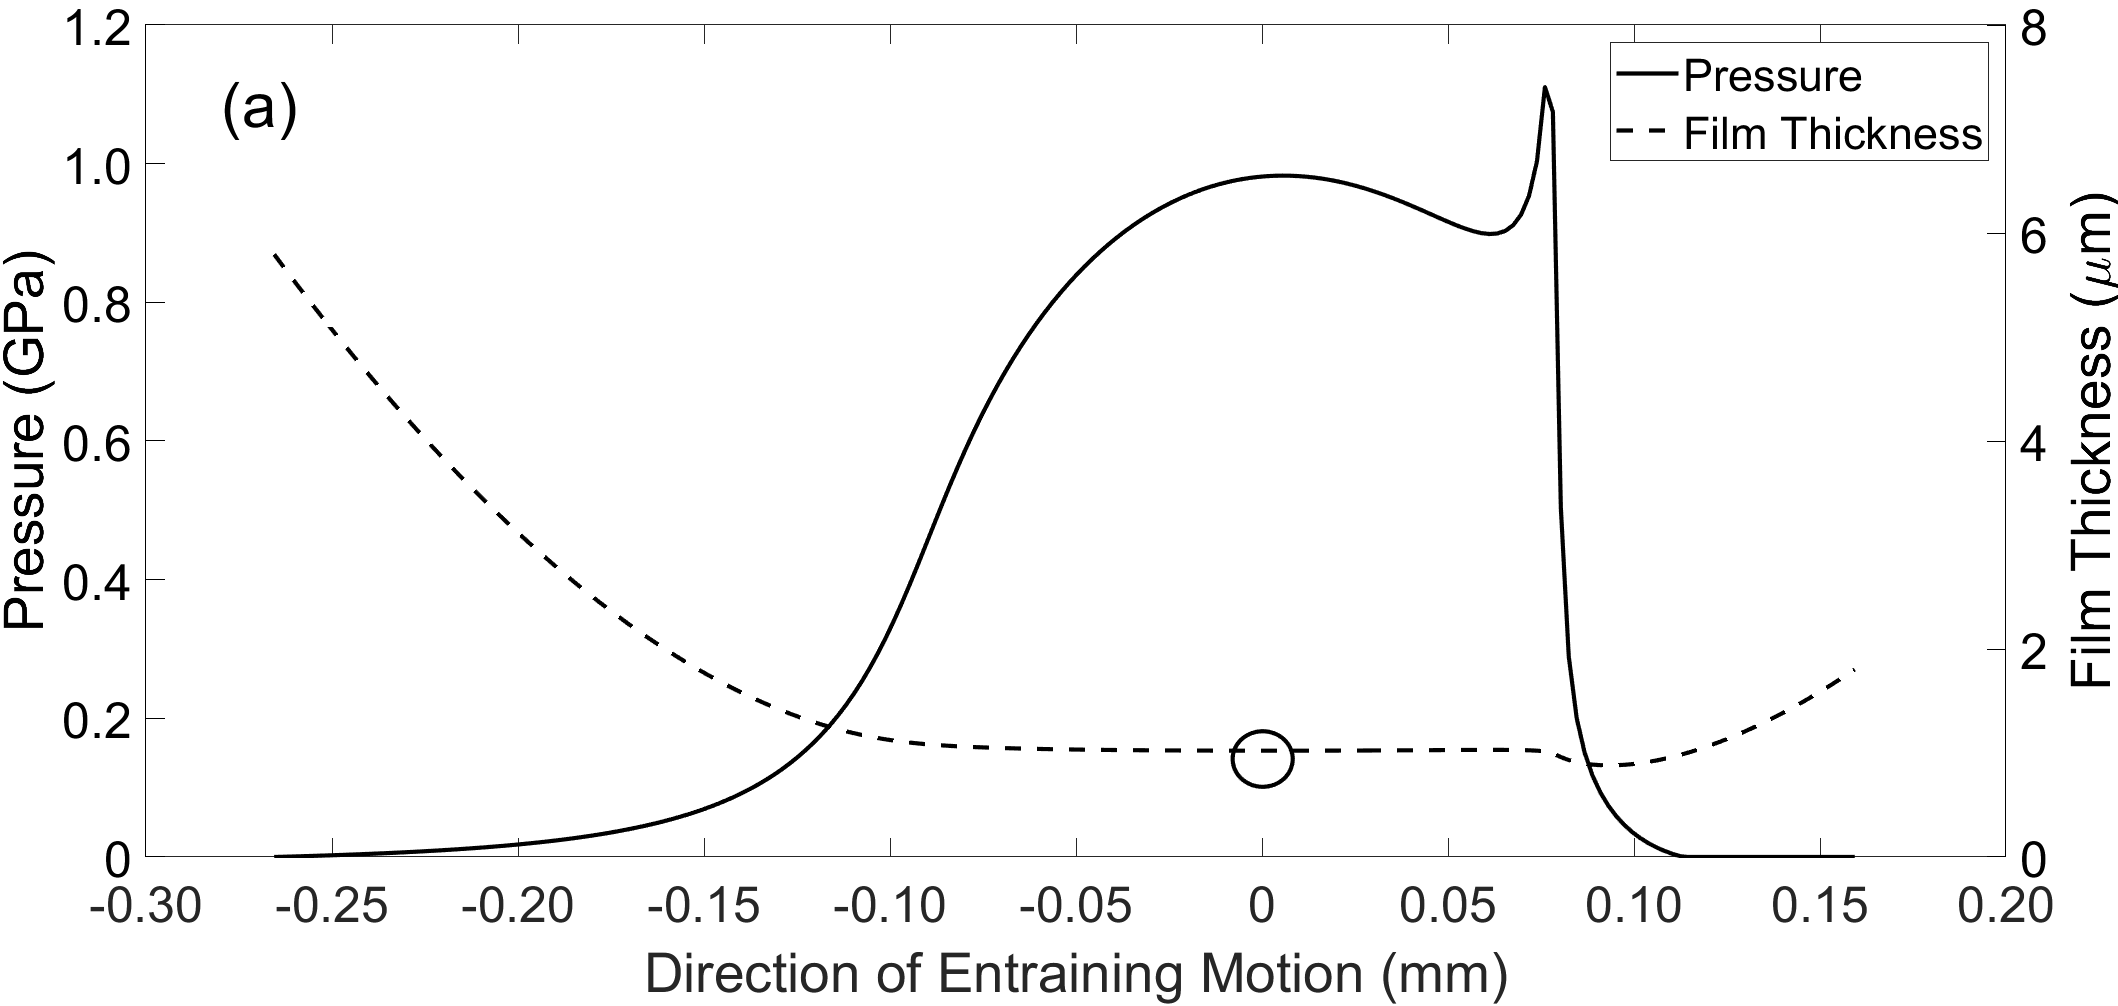
\includegraphics[width=\textwidth]{ExpTribo Figure 18a.png}
		\caption{}
		\label{NodeA}
	\end{subfigure}
	\hfill
	\begin{subfigure}[b]{0.49\textwidth}
		\centering
		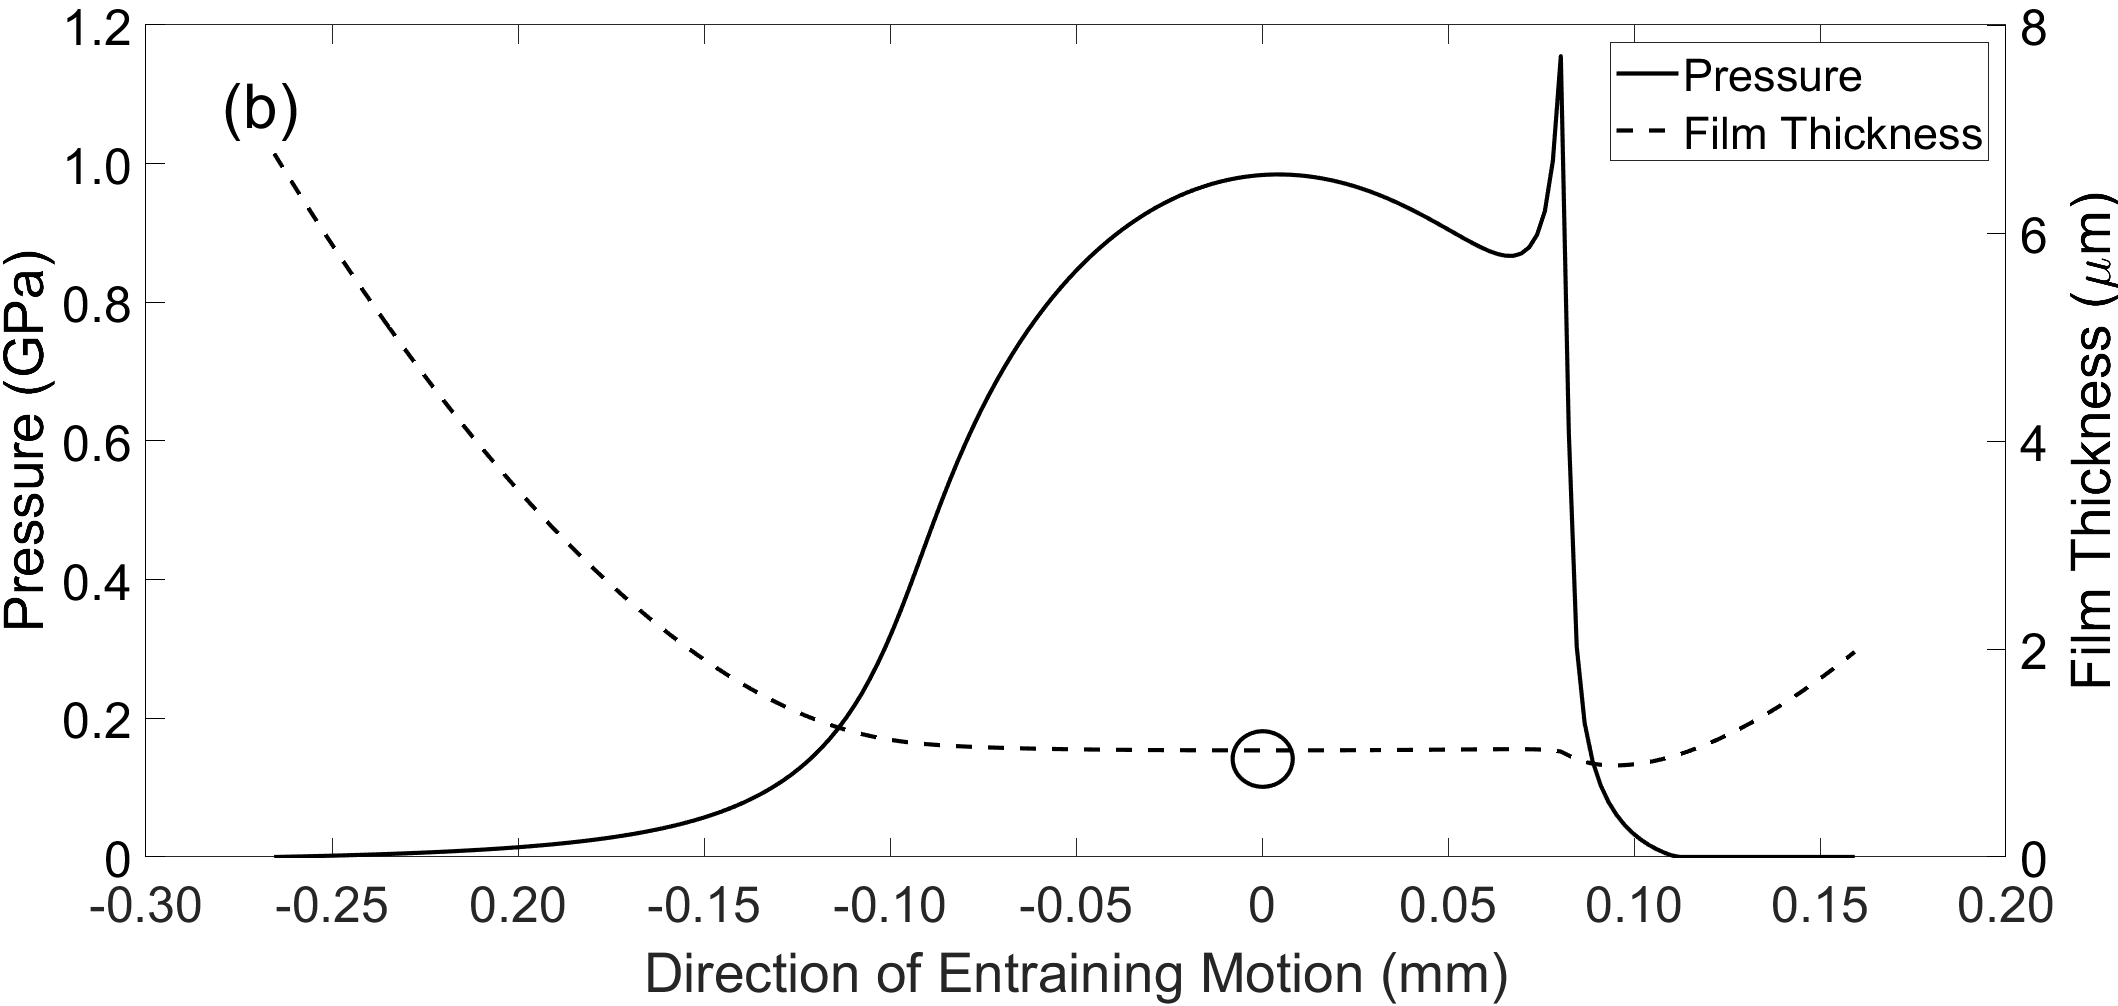
\includegraphics[width=\textwidth]{ExpTribo Figure 18b.png}
		\caption{}
		\label{NodeB}
	\end{subfigure}
	\hfill
	\begin{subfigure}[b]{0.49\textwidth}
		\centering
		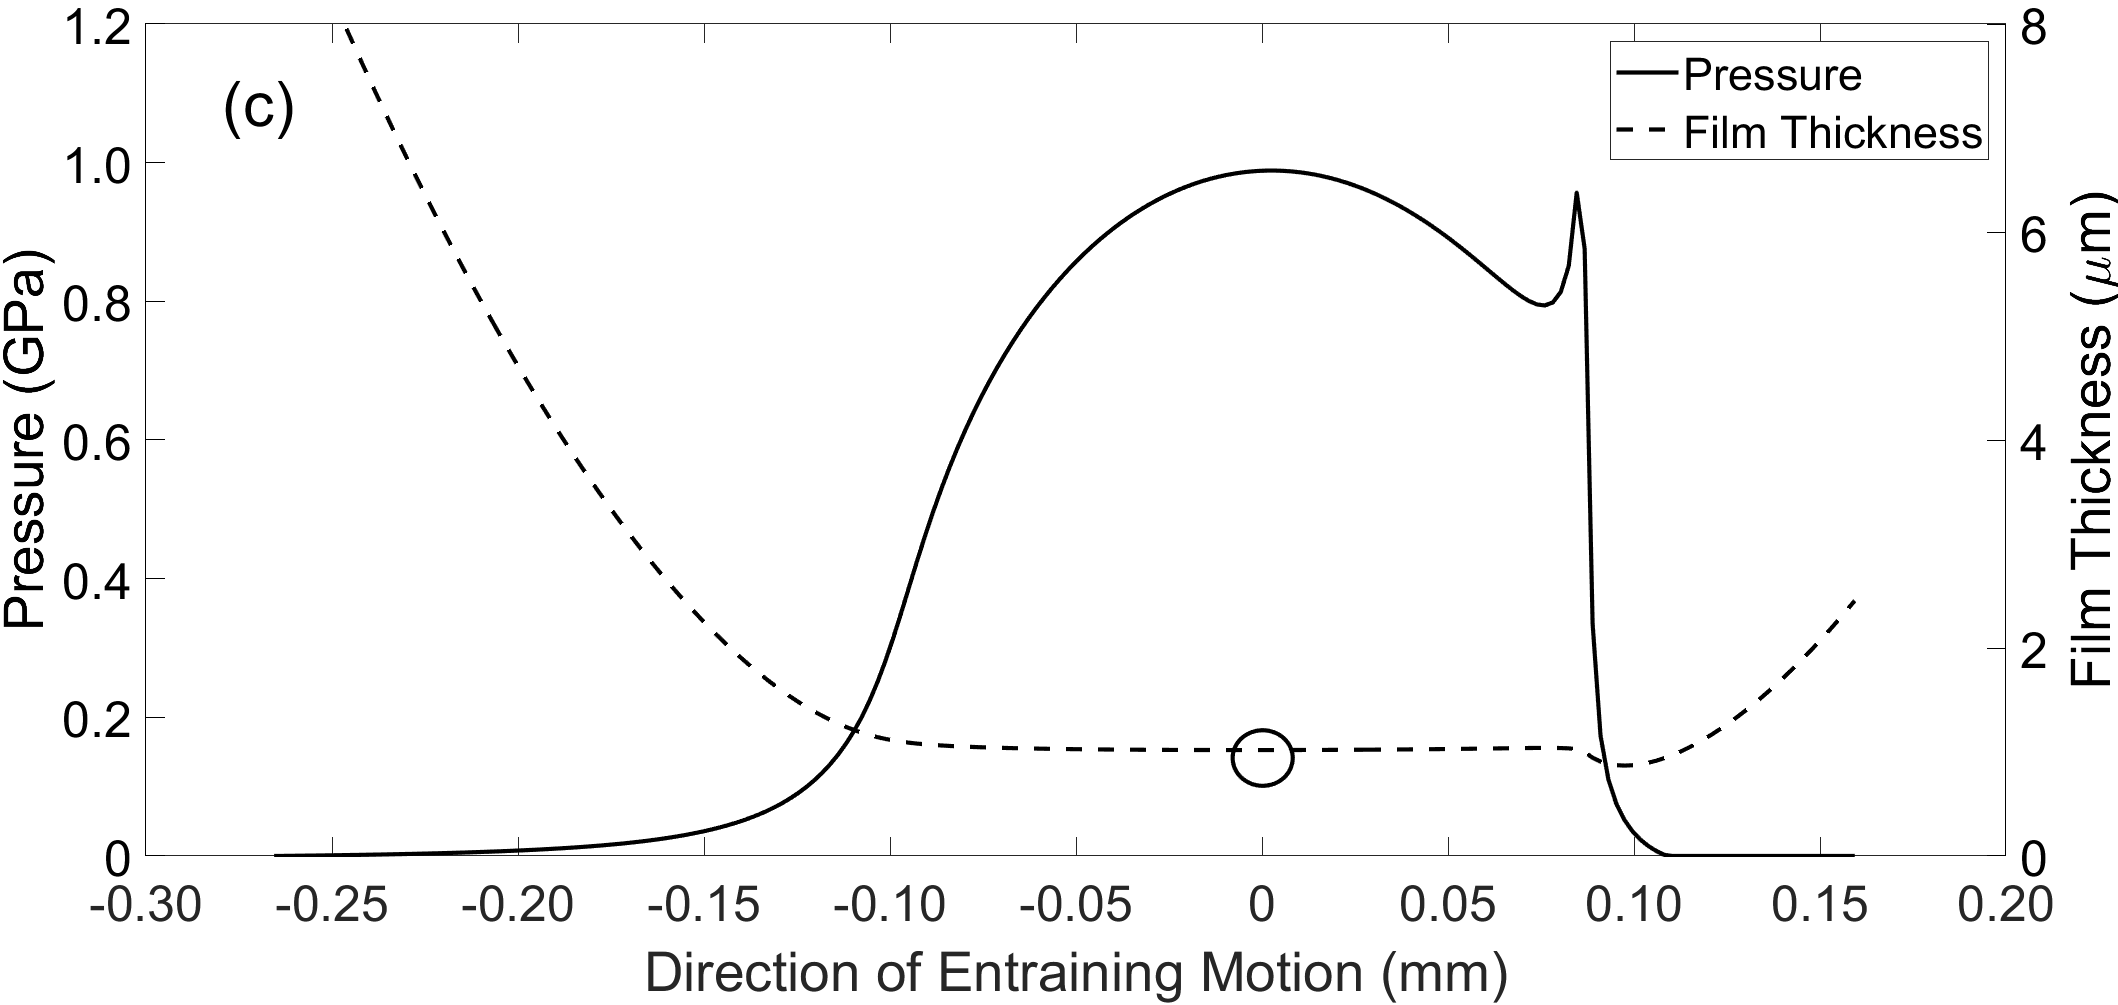
\includegraphics[width=\textwidth]{ExpTribo Figure 18c.png}
		\caption{}
		\label{NodeC}
	\end{subfigure}
	\hfill
	\begin{subfigure}[b]{0.49\textwidth}
		\centering
		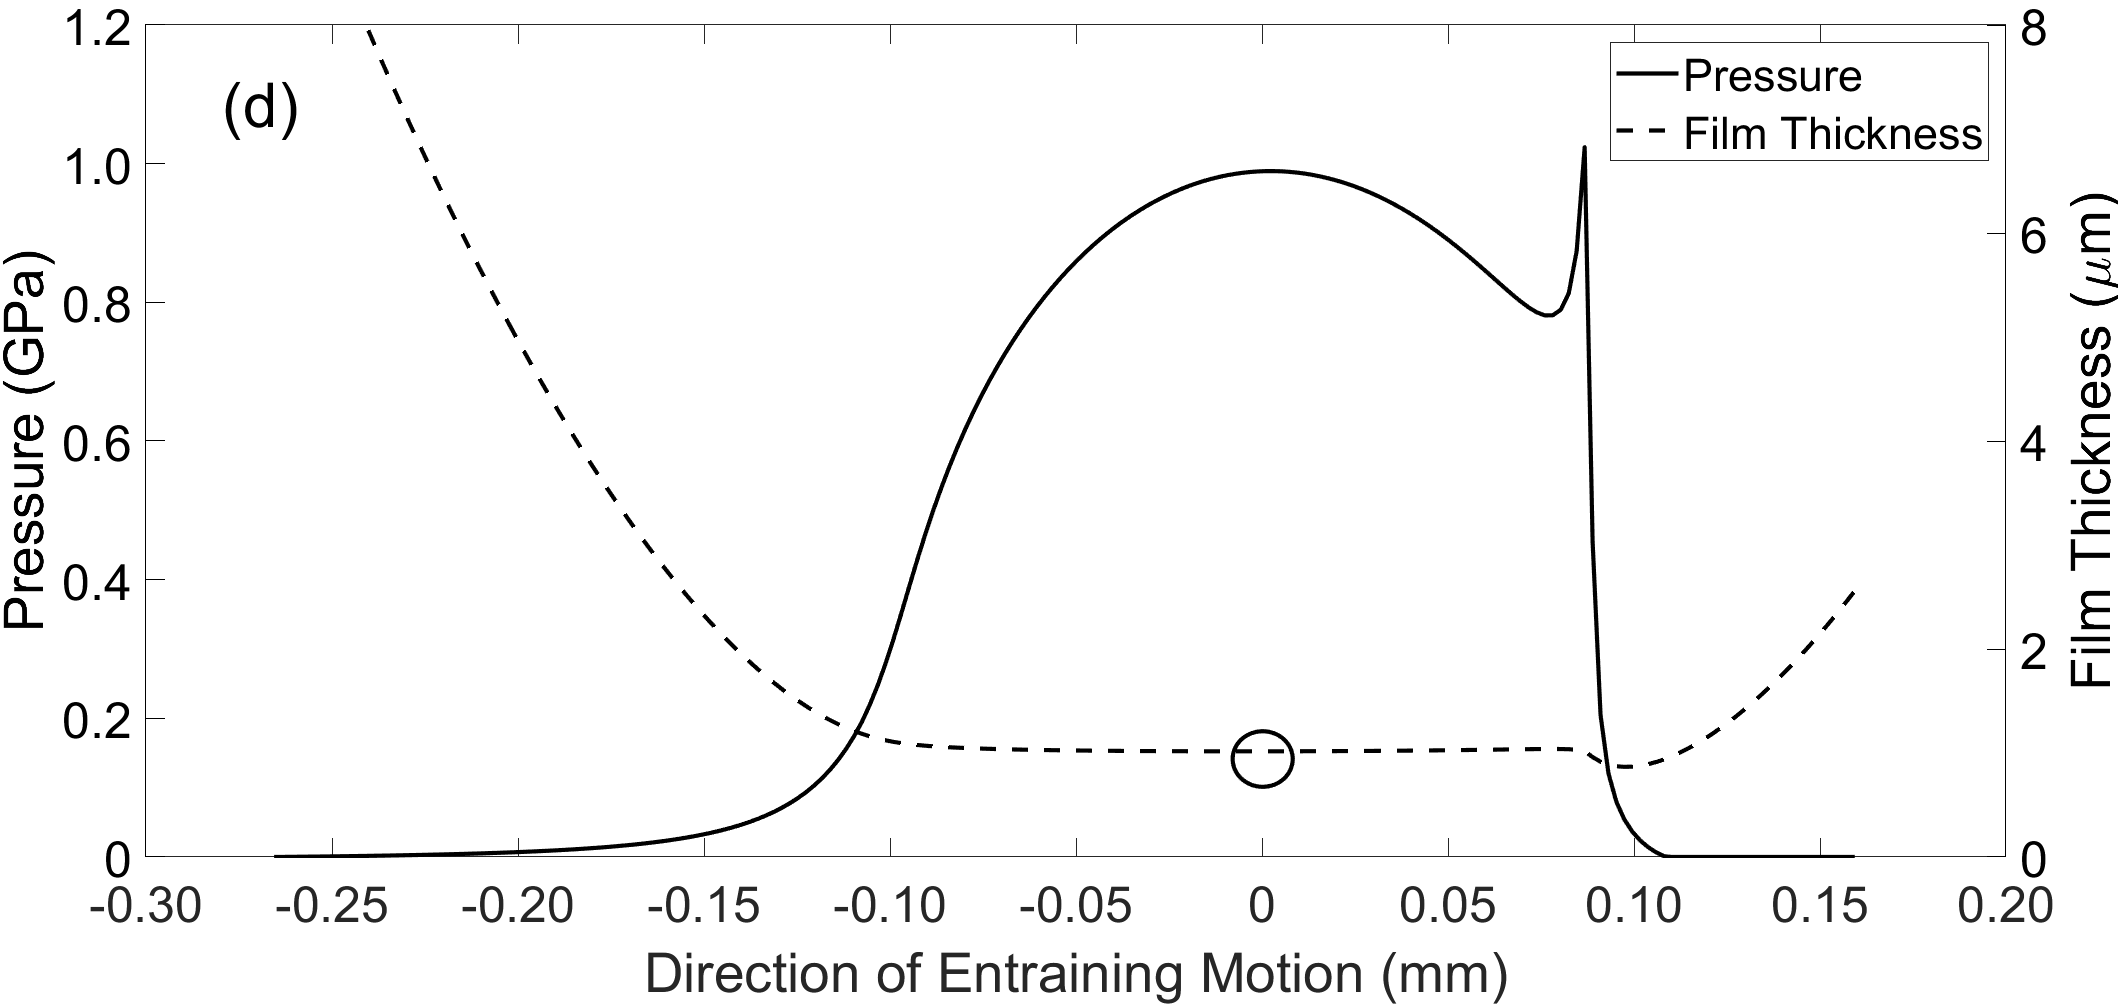
\includegraphics[width=\textwidth]{ExpTribo Figure 18d.png}
		\caption{}
		\label{NodeD}
	\end{subfigure}
	\hfill
	\begin{subfigure}[b]{0.49\textwidth}
		\centering
		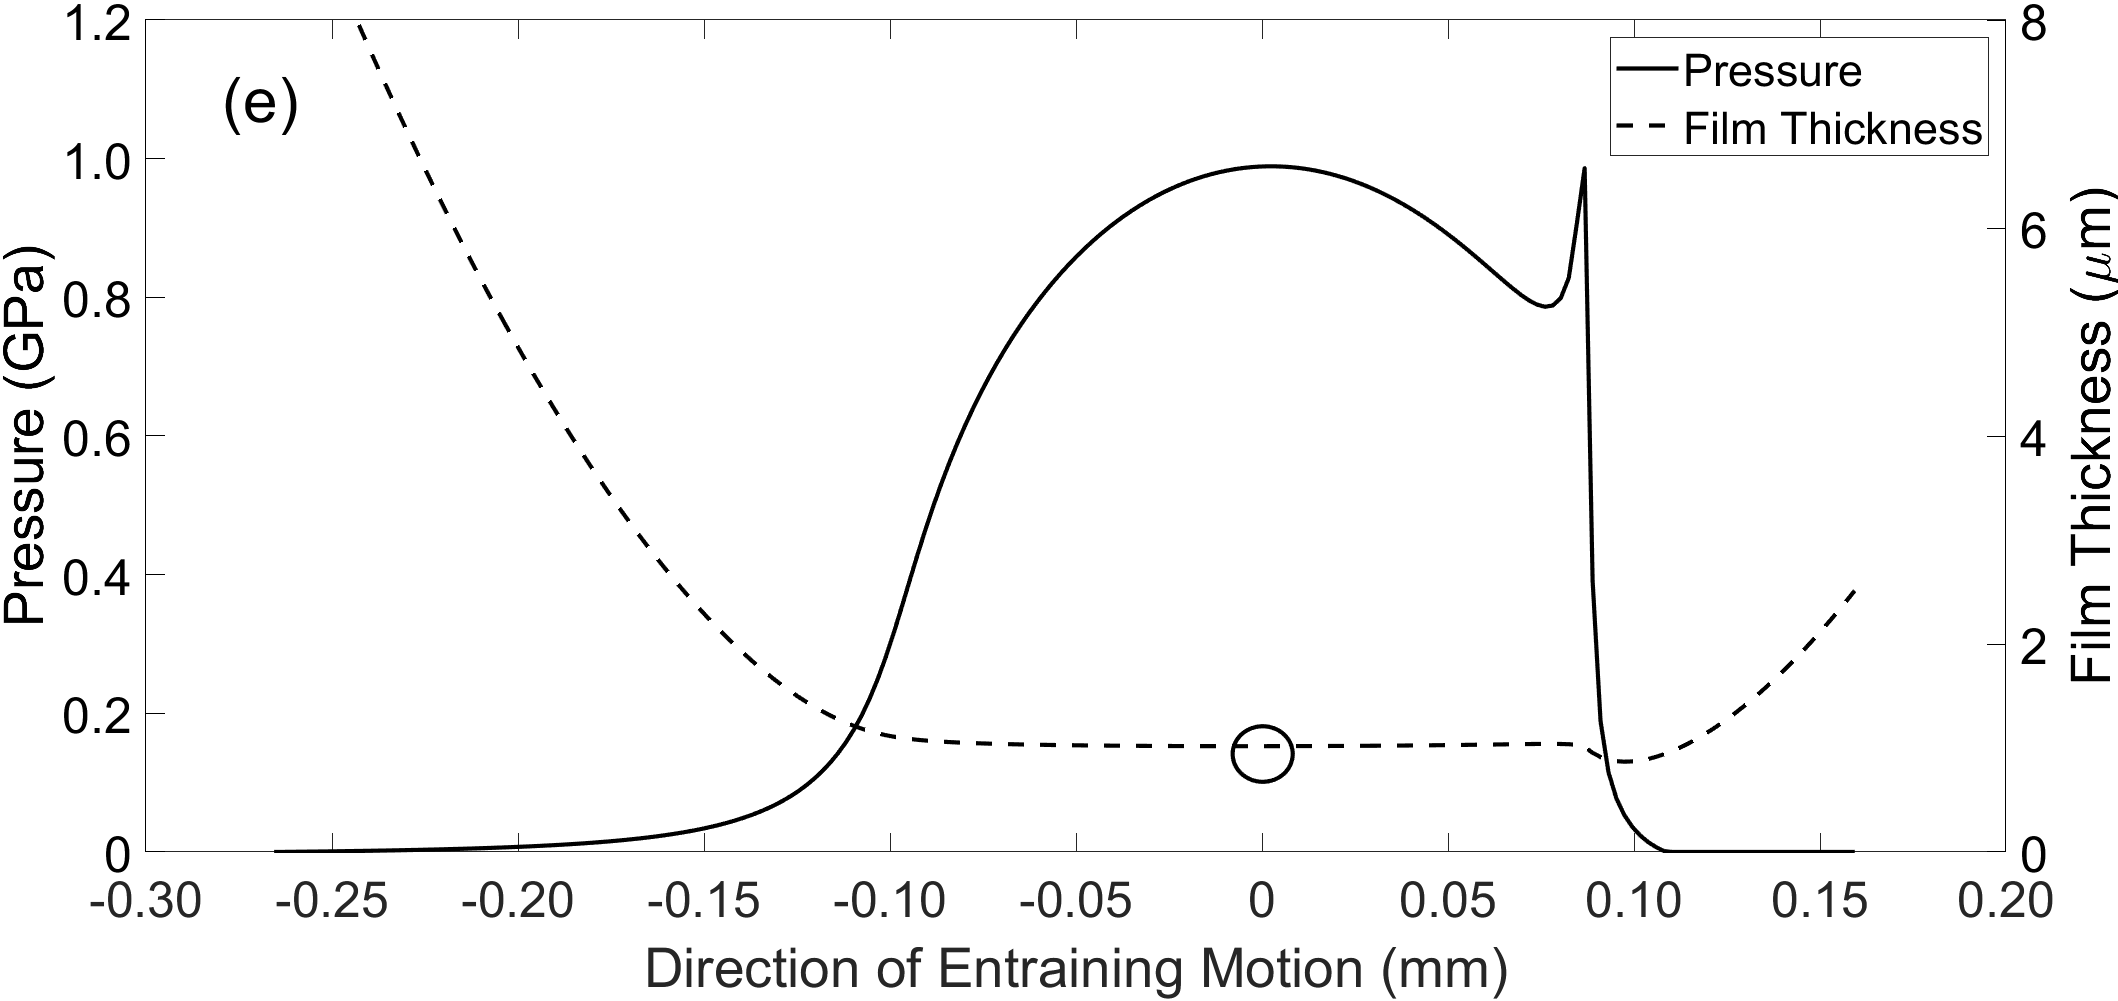
\includegraphics[width=\textwidth]{ExpTribo Figure 18e.png}
		\caption{}
		\label{NodeE}
	\end{subfigure}
	\hfill
	\begin{subfigure}[b]{0.49\textwidth}
		\centering
		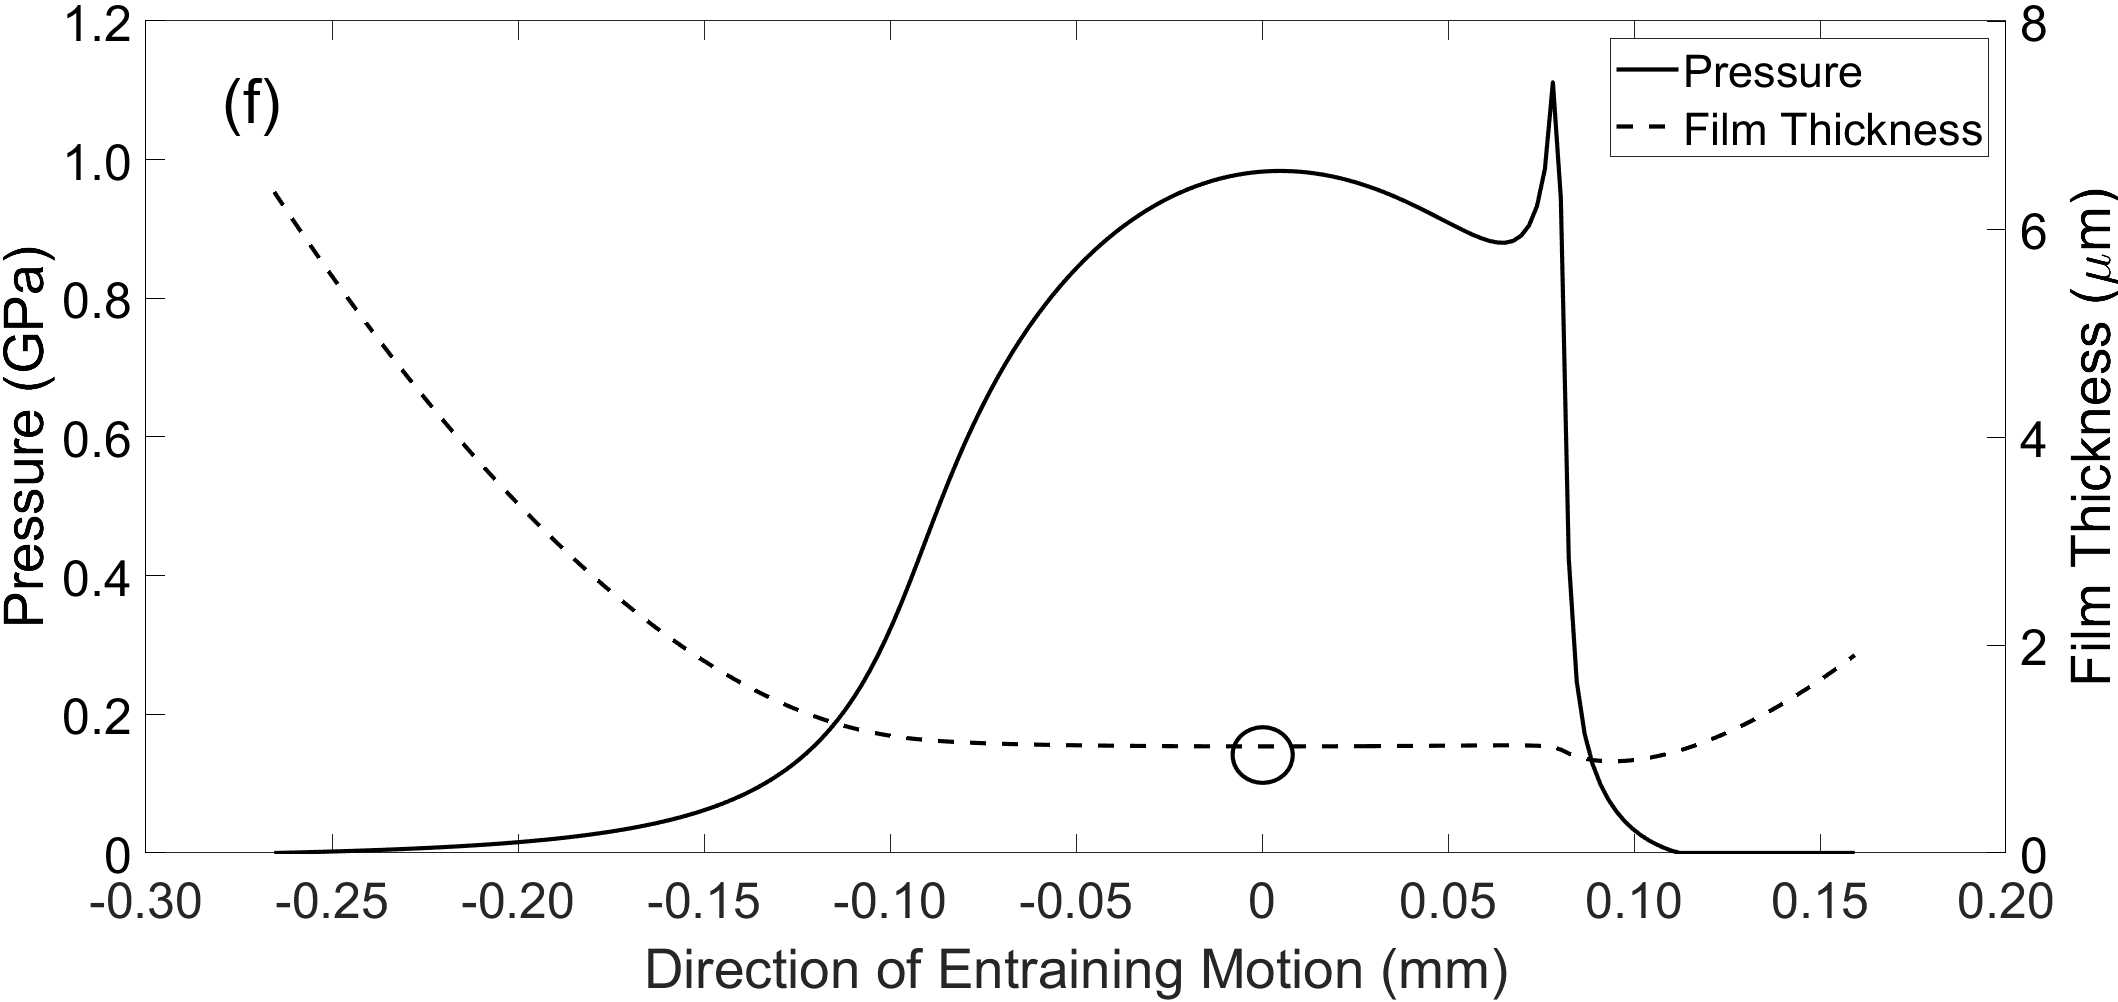
\includegraphics[width=\textwidth]{ExpTribo Figure 18f.png}
		\caption{}
		\label{NodeF}
	\end{subfigure}
	\caption{EHL pressure and film thickness distributions: a) Node 1, b) Node 2, c) Node 3, d) Node 4, e) Node 5, f) Node 6}
	\label{EHL pressure and film thickness distributions}
\end{figure}

In each of these plots, it is possible again to see the central film thickness drop as the roller enters, then exits the loaded region. These central film values are represented by circles in Figure 18. Agreement between the extrapolated film formulae and the numerical model for calculating central film values are presented in Table \ref{Extrapolated film formulae and numerical model central film thickness comparison}. This confirms the validity of using extrapolated film thickness equation in the implicit tribological model. It is shown that the central nodes which correspond to the higher loads in the loaded region have the lowest percentage difference in comparison to the lightly loaded nodes at the outer edges.

\begin{table*}
	%\captionsetup{justification=centering}
	\caption{Extrapolated film formulae and numerical model central film thickness comparison}
	\label{Extrapolated film formulae and numerical model central film thickness comparison}
	\centering
	\renewcommand{\arraystretch}{1.5}%
	\begin{tabular}{|P{0.1\textwidth}|P{0.3\textwidth}|P{0.3\textwidth}|P{0.3\textwidth}|}
		\hline
		\textbf{Node} & \textbf{Extrapolated Formulae Central Film Thickness ($\mu m$)} & \textbf{Numerical Model Central Film Thickness  ($\mu m$)} & \textbf{Percentage Difference (\%)} \\ [0.5ex]
		\hline
		1 & 1.142 & 1.026 & 11.3 \\ [0.5ex]
		\hline
		2 & 1.122 & 1.025 & 9.46 \\ [0.5ex]
		\hline
		3 & 1.075 & 1.019 & 5.49 \\ [0.5ex]
		\hline
		4 & 1.068 & 1.016 & 5.11 \\ [0.5ex]
		\hline
		5 & 1.072 & 1.018 & 5.30 \\ [0.5ex]
		\hline
		6 & 1.122 & 1.025 & 9.46 \\ [0.5ex]
		\hline
	\end{tabular}
\end{table*}

\section{Conclusions}

A new methodology comprising experiments and numerical modelling has been developed to allow component and conjunction level tribo-dynamic analysis of a roller bearing under speeds and loading conditions previously not reported. The experimental data contain the physics of the dynamics and tribology within the bearing, negating the need for a simplified and computationally intensive dynamic bearing model. The tribological conditions at the contact between an individual roller and raceways are numerically analysed. All possible lubrication regimes, including mixed-EHL and hydrodynamic, are considered as the roller passes through loaded and unloaded regions.

The presented research investigates a new range of working conditions under high speeds, representative of modern electrified powertrains. This study helps to understand the prevailing regimes of lubrication as well as range of tribological quantities. Additionally, the interaction of tribological behaviour with dynamics of the system is investigated. The deeper and comprehensive understanding of these matters will support objective development of electrified powertrains in the future towards higher efficiency, durability and NVH refinement. The acquired knowledge and understanding will also support future developments of predictive tools by understanding the interaction of tribology and dynamics and the significance of considering this multi-physics interaction. The following conclusions can be made based on presented results:

\begin{enumerate}
	\item The contact experiences an order of magnitude increase in film thickness across the speed sweep. This highlights the necessity of implicitly including the lubricant film in any predictive tribo-dynamic model; an approach that is not reported on in open literature for high-speed dynamic roller bearing analysis.
	\item A comparison between the dry and lubricated contact model further reinforces the need to include the lubricant film in high-speed roller bearing analysis, with percentage differences in load between both models up to 149\% at 15 000 rpm. Neglecting this film by using the common dry Hertzian approach would lead to an underestimation of the total load at the roller-race contact. 
	\item At higher speeds, such as those present in modern electric powertrains, it is shown that the growth of the lubricant film must be included implicitly within the dynamic bearing analysis.
	\item The load values obtained from the lubricated tribological model have been used explicitly within a 1-dimensional EHL model to calculate the pressure distribution and film thickness across the contact. The workflow of using an explicit EHL model based on the analytical tribological contact mechanics is valid, with good agreement between central film thickness values for both. 
	\item The explicit EHL approach significantly improves the computational efficiency of the model whilst maintaining accuracy, since only the central value of the film is required in the load calculation. This can be implicitly coupled to broaden the scope of the analysis that is being performed.
\end{enumerate}
\chapter{Modelling Lubricated Bearings in a Flexible Multi-Body Dynamic Environment}
\label{Lubricated FMBD}

\section{Preface}

This chapter presents a new flexible dynamic model for drive systems comprising lubricated bearings operating under conditions representative of electrified vehicle powertrains. The multi-physics approach importantly accounts for the tribological phenomena at the roller–race conjunction and models their effect on shaft-bearing system dynamics. This is achieved by embedding a non-linear lubricated bearing model within a flexible system level model; this is something which has not, to the authors’ knowledge, been reported on hitherto. The elastohydrodynamic (EHL) film is shown to increase contact deflection, leading to increased contact forces and total bearing stiffness as rotational speeds increase. Results show that for a 68~$Nm$ hub motor operating up to 21~000~$rpm$, the input bearing EHL film reaches a thickness of 4.15~$\mu m$. The lubricant entrainment increases the roller–race contact deflection, causing the contact stiffness to increase non-linearly with speed. The contribution of the lubricant film leads to a 16.6\% greater bearing stiffness at 21~000~$rpm$ when compared to conventional dry bearing modelling methods used in current multi-body dynamic software. This new methodology leads to more accurate dynamic response of high-speed systems necessary for the next generation of electrified vehicles. 

\section{Introduction}

Simulating electrified powertrains using flexible multi-body dynamic (FMBD) models can enable substantial cost and time savings for automotive manufacturers due to a reduced need for physical prototyping. With increasing complexity and operational speeds of these systems, the accuracy at the component level is of major importance. Bearings are crucial structural components and their dynamic response significantly affects the behaviour of the interconnected structures.

Modern electrified motors and transmissions operate at considerably higher speeds and lower loads than conventional powertrains \cite{Cai2021}. This leads to much higher lubricant entrainment velocities at the roller–race conjunction of the bearings. Consequently, the elastohydrodynamic (EHL) film thickness can be of the same order of magnitude and often exceed that of the contact deformation predicted by dry Hertzian assumptions; hence, non-lubricated analyses are no longer valid.
The operating conditions of roller bearings in modern electric vehicle (EV) powertrains require dynamic modelling to capture system transients such as time-varying input forces, acceleration and eccentricity. Early quasi-static bearing models \cite{Stribeck1907} \cite{Palmgren1959} \cite{Jones1960} \cite{Harris1984}, are only applicable under steady-state operating conditions; however, the static equilibrium solutions \cite{Andreason1973} \cite{Liu1976} \cite{DeMul1989_1} are of use to calculate load-deflection and individual element loading within dynamic models. Simplified 2-degree of freedom dynamic models \cite{Walters1971} consider the purely in-plane motion of the rolling elements in the radial and lateral directions of the bearings for the investigation of the frequency response to defects \cite{Ahlgren2015b}, the varying compliance effect \cite{Sunnersjo1978} and the radial loading affects \cite{Matsubara1988}. These models increase in complexity up to 5 degrees of freedom (DOF) to observe moment loading and centrifugal effects \cite{Rahnejat2004} \cite{Gupta1979}. These analyses assumed a dry contact between the rolling elements and races, which was considered to be valid at lower speeds and high loads. This, however, neglects the effect of the lubricant film thickness in the contact mechanics and thus underestimates the contact deflection and hence the load.

Based on the experimental and numerical findings \cite{Questa2020} \cite{Stone1982} \cite{Dietl1997}, the EHL film can be shown to increase the bearing stiffness, which continues to rise non-linearly with speed. It is therefore clear that the lubricant film in roller bearings operating at high speeds must be implicitly included in dynamic analyses.

As stated by Bizarre et al. \cite{Bizarre2018}, there are few studies in the open literature that combine the stiffness and damping of an EHL contact with classical bearing dynamics. Early lubricated bearing models use extrapolated formulae to provide a relationship between the load share and film thickness at each element’s contact with the bearing raceways \cite{Rahnejat1985}. Aini et al. \cite{Aini2002} implemented the extrapolated film approach from the work of Rahnejat and Gohar \cite{Rahnejat1985} into a five-DOF bearing equilibrium model. The work computes the deformation at each roller–race contact, combining the EHL film thickness with the elastic deformation of the contacting solids. The force–displacement relationship is shown to follow a non-linear trend. Mohammadpour et al. \cite{Mohammadpour2015c} employed a similar implicit tribodynamic analysis and then utilised a full numerical EHL analysis explicitly for further tribological studies. In their analysis, input shaft speeds of 209~$rad/s$ resulted in much slower entrainment velocities than are applicable for electrified powertrain analyses.

Sopanen and Mikkola \cite{Sopanen2003_1} modelled the influence of various surface characteristics on bearing dynamics, including contributions from surface waviness, roughness, localised and distributed effects. Their six-DOF model accounts for the Hertzian contact deformation and the EHL film implicitly within the contact. This model was embedded in a multi-body dynamic (MBD) software to utilise its mathematical capabilities. This work does not, however, demonstrate the effect that the EHL film has on bearing stiffness, and the effect on system dynamics using flexible bodies is not analysed \cite{Sopanen2003_2}. Sawalhi and Randall \cite{Sawalhi2008} used a constant preload approach to imitate the stiffening effect of the film. Whilst this effective preload captures the increased contact stiffness due to the presence of the EHL film, the film thickness does not vary based on the contact conditions.

More recently, Liu and Shao \cite{Liu2017b} investigated the effects of surface waviness, including the effect of the lubricant film using an equivalent stiffness model. Nonato and Cavalca \cite{Nonato2014} presented a methodology to model EHL contacts using a set of non-linear springs and viscous dampers. Bizarre et al. \cite{Bizarre2018} applied this lubricated non-linear force contact to a five-DOF model of an angular contact ball bearing. This enabled a combined solution scheme for the bearing force equilibrium and the EHL contact. The formulated system of equations was solved, achieving force equilibrium for each rotation of a bearing under constant external load. The authors of this study noted the interest of combining such models within FMBD system level models.

None of the combined models above are embedded within a system level model comprising flexible bodies, and the effect of the change in the contact stiffness due to the lubricant film is not investigated at the system level. Furthermore, the high-speed operation and time-varying loads representative of electrified vehicle transmissions are not considered.

Presented in this chapter, for the first time in the open literature, a coupled simulation approach to combine an implicit lubricated bearing model within a high-speed system level FMBD model. The time-varying system operating conditions reflect that of an electrified powertrain. The kinematic behaviour of a flexible shaft at each time step of a dynamic simulation is passed to the bearing model. A contact slicing method \cite{Andreason1973} is employed to calculate the reaction forces of the individual rolling elements based on the roller–race contact deflection \cite{Lundberg1949}. The total deflection is influenced by the thickness of the EHL film within the contact, which is implicitly included within the analysis through an iterative procedure. The resulting race forces are returned to the system level model and the equations of motion are solved at each time step. Comparisons are made between modelling the bearings as dry and lubricated. The dynamic results including acceleration, force magnitudes and stiffness variations have been obtained for realistic loading conditions of a 54~$kW$ electric hub motor up to speeds of 21~000~$rpm$.

\section{Methodology}

A co-simulation methodology combines a system level model of a flexible shaft and rigid housing, developed in AVL EXCITE\textsuperscript{TM}, with component level models of the lubricated bearings, developed in MATLAB and Simulink. Operating conditions such as rotational speed and external forces are defined in the system level model. Time step, iteration accuracy and simulation length are also defined. Material, geometric and rheological properties of the bearings are defined in the component level model. The kinematic conditions from the system level model (i.e., displacements and velocities in all active degrees of freedom) are passed to the component level model at each time step. For each individual rolling element, the non-linear force–deflection relationship is employed in conjunction with the EHL film calculations to compute the contact reaction force between the roller and race. The resultant force on the inner bearing race due to the contact forces and orbital positions of all elements is then returned to the system level model. The equations of motion are then solved, and the time step is advanced once numerical convergence is achieved. A flowchart of these models representing each time step of the simulation is shown in Figure \cite{Flowchart of models}.

\begin{figure}
	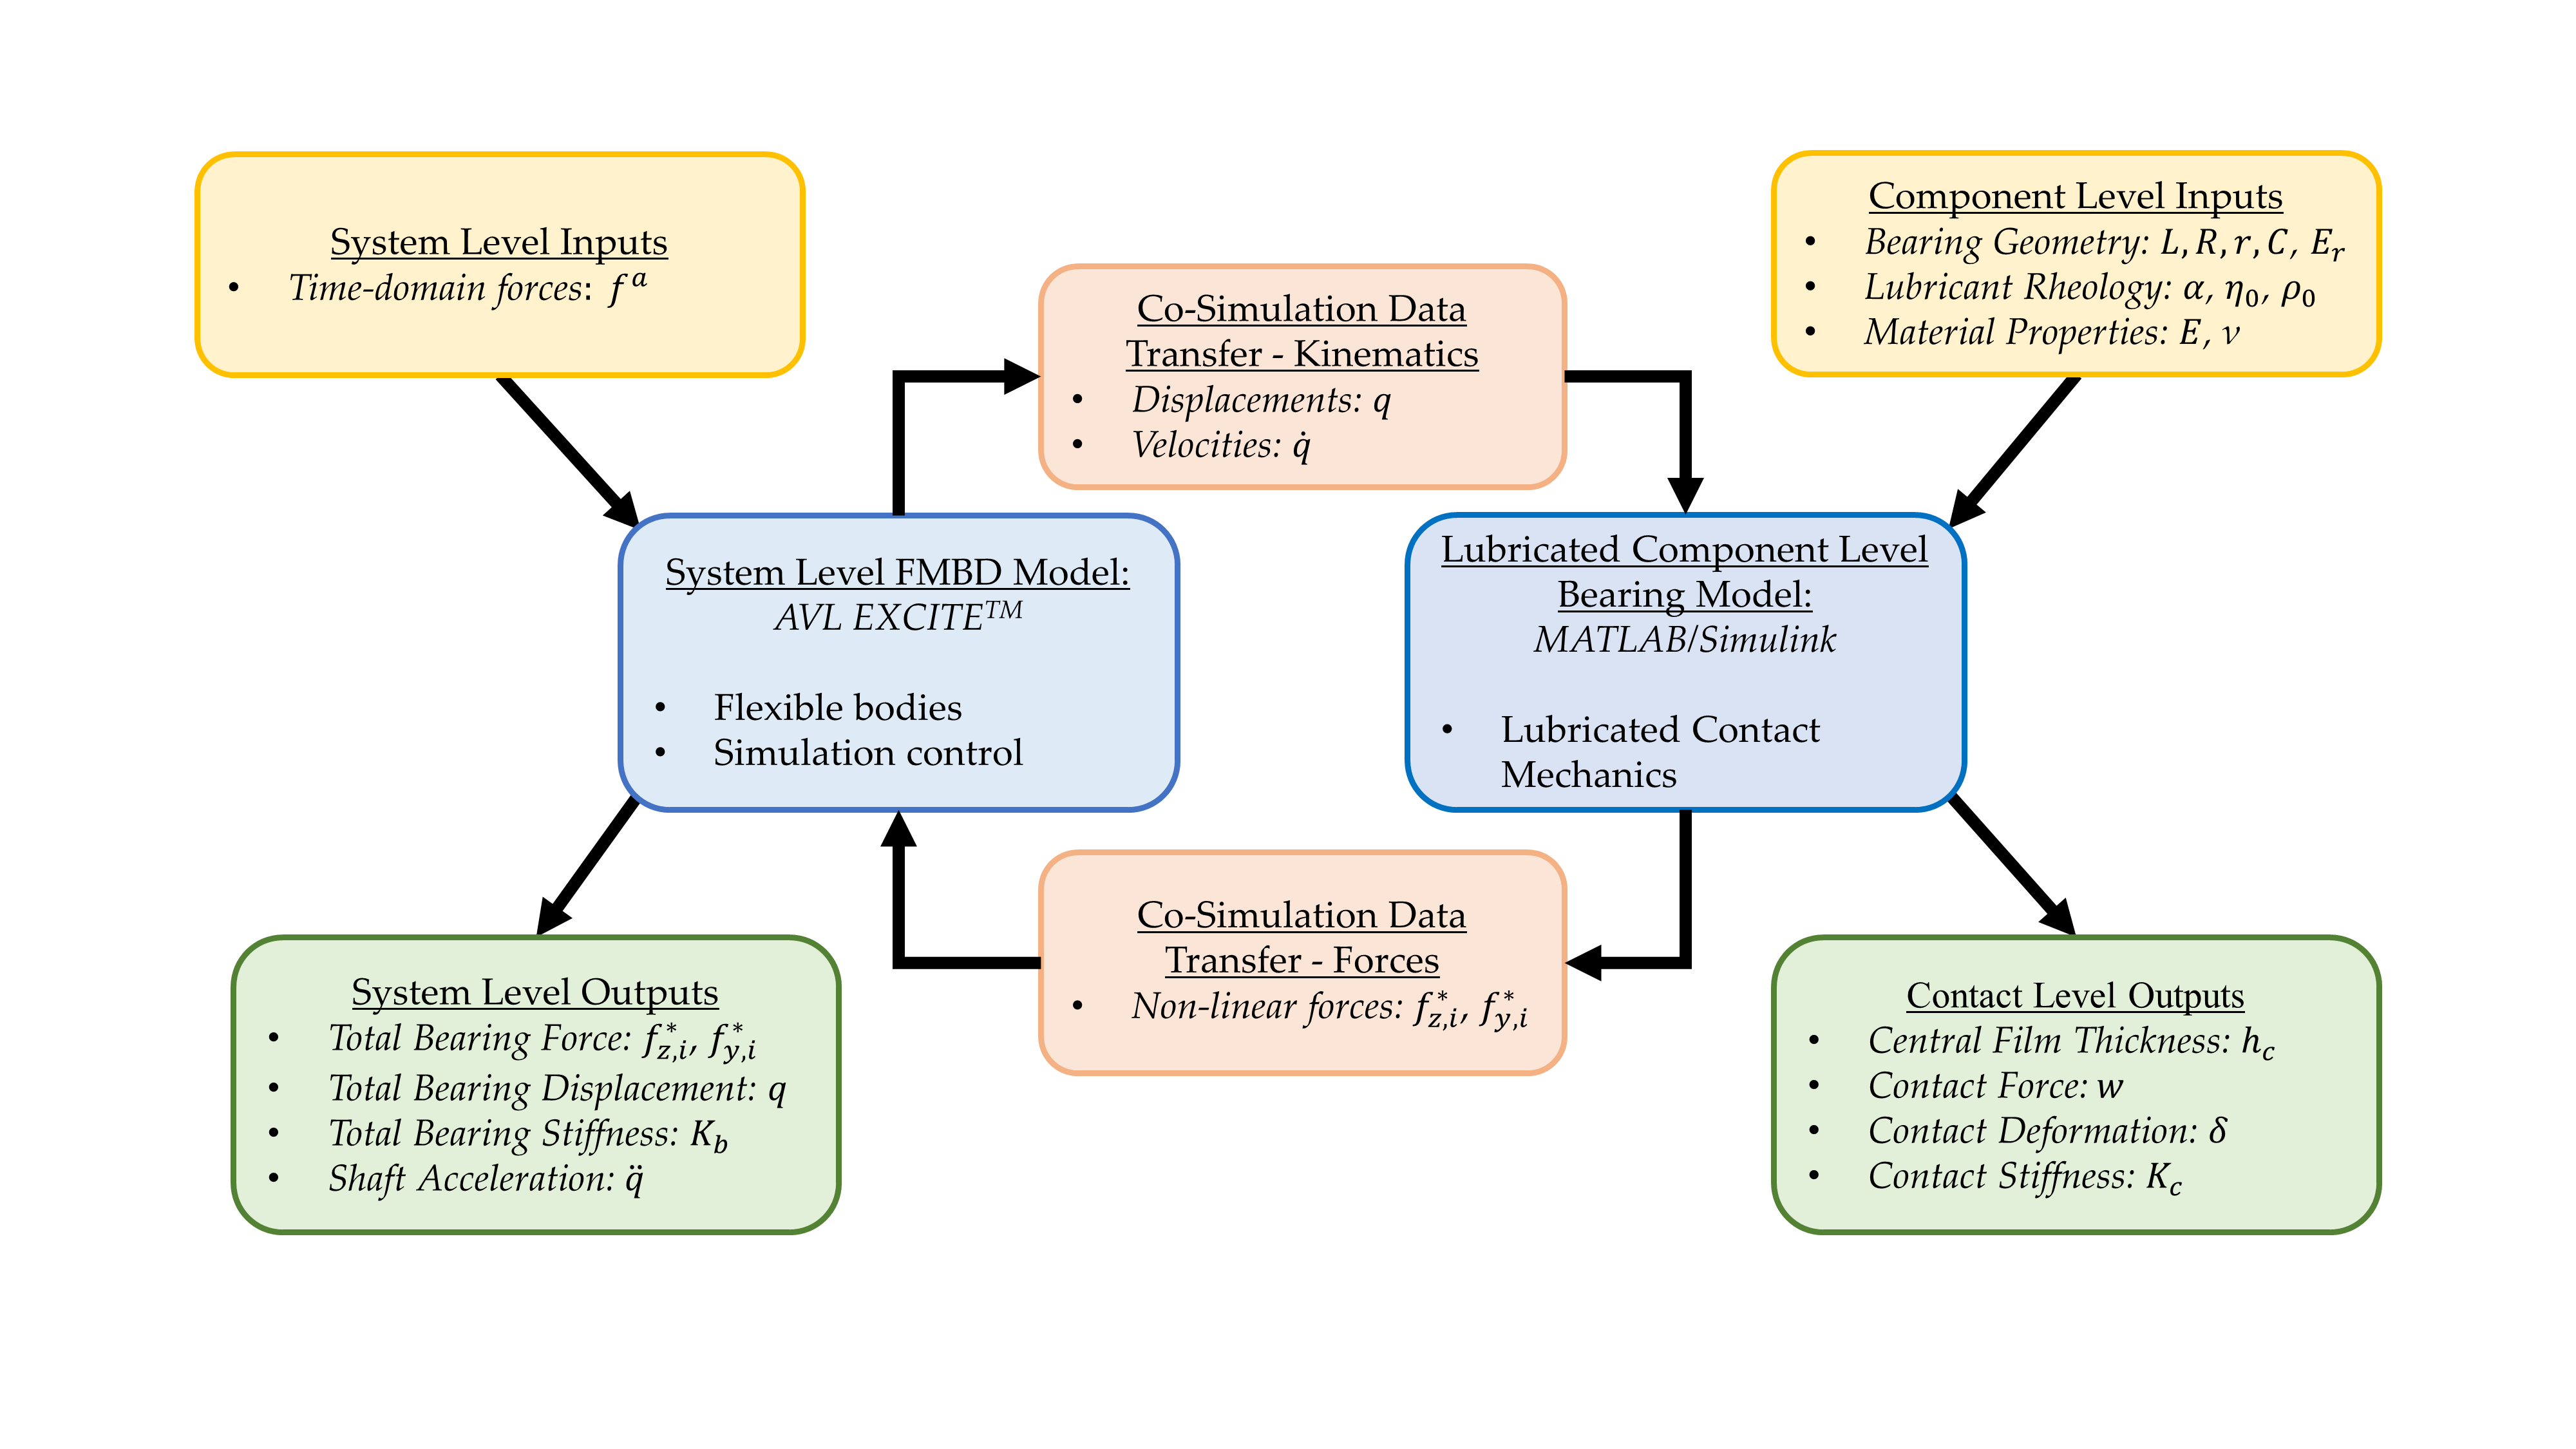
\includegraphics[width=150mm]{FlexiTribo Figure 1. Flowchart of Models.png}
	\caption{Flowchart of models.}
	\label{Flowchart of models}
\end{figure} 

\section{System Level Flexible Model}

The system level model consists of a flexible shaft, supported by two cylindrical roller bearings in a rigid housing (see Figure \ref{System level model schematic}). The shaft is 472.5~$mm$ between bearing centres, with a 50~$mm$ main diameter and 25~$mm$ diameter bearing seats. The cylindrical roller bearings act as interference elements between the shaft and housing. The shaft can exhibit lateral motion in both vertical ($z$) and horizontal ($y$) directions and rotation about the $x$-axis (see Figure \ref{System level model schematic}). External load is applied at the shaft centre as a time-varying input force, to simulate the gear mesh excitation, or as a static load. The rotational speed is input as a boundary condition.

\begin{figure}  
	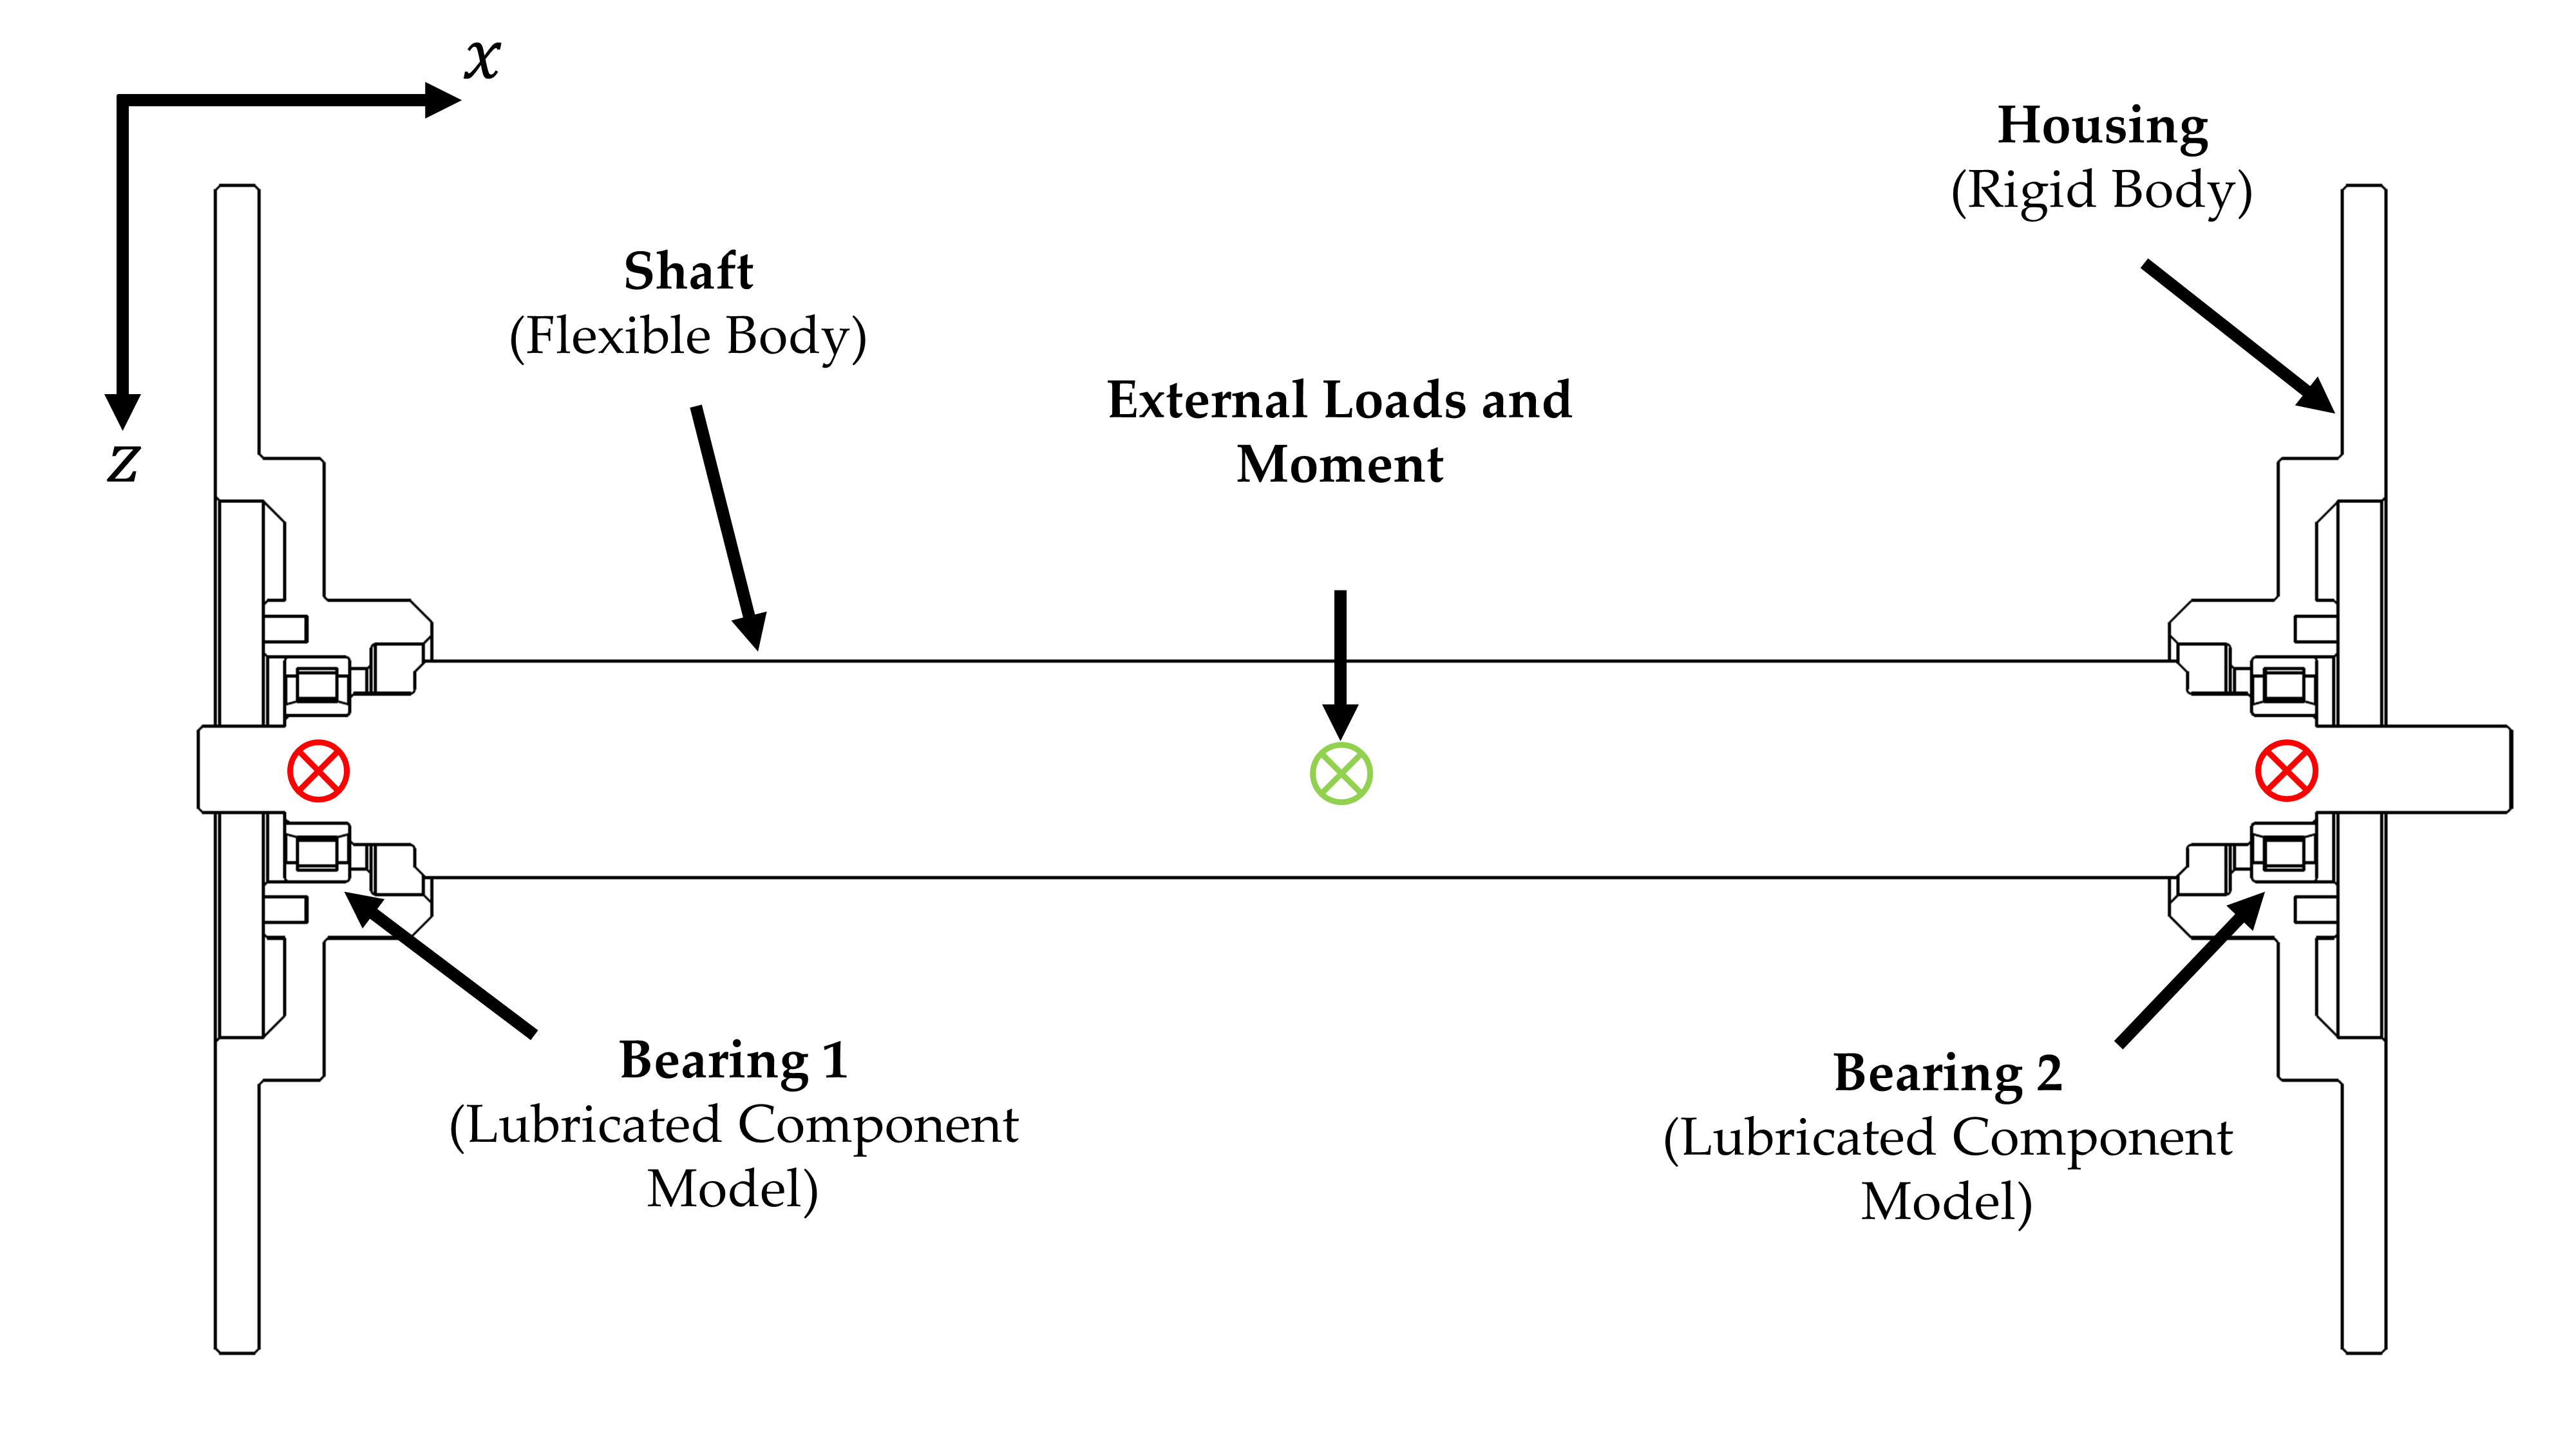
\includegraphics[width=150mm]{FlexiTribo Figure 2. System Level Model Schematic.png}
	\caption{System level model schematic.}
	\label{System level model schematic}
\end{figure} 

In typical configurations containing flexible structures, it is possible for both the inner and outer races of a rolling element bearing to move when subject to load. For this analysis, however, it is sufficient to fix the outer race in space and consider only the displacement of the inner bearing race \cite{DeMul1989_2}. The housing in this study is treated as a rigid body of infinite stiffness; therefore, the race dynamics of the bearing are influenced only by the motion of the flexible shaft in the model. The loading on the inner race is reacted by the rolling elements on the inner raceway; this must therefore be solved to achieve a dynamic equilibrium.

Within the model, the shaft is treated as a body having linear elastic behaviour and the housing is treated as rigid. The bearings are modelled via non-linear contact forces acting between the shaft and housing.

The shaft is represented by a condensed finite element model and is discretised into a sufficiently high number of partial masses \cite{Parikyan2001}. The total elastic deformation of the shaft is represented by translational and rotational displacement components of these individual partial masses. The mathematical modelling used in the FMBD solver is based on Newton’s equations of motion and Euler’s equation of angular momentum, respectively:

\begin{equation}\label{NewtonFMBD}
	m_i \frac{\partial^2 x_i^{A b s}}{\partial t^2}=f_{F, i}^{A b s}
\end{equation}

\begin{equation}\label{EulerFMBD}
	\frac{\partial}{\partial t}\left(I_{C, i}^{A b s} \omega_i^{A b s}\right)=f_{M, i}^{A b s}
\end{equation}

where $m_i$ and $I_{C, i}^{A b s}$ represent the mass and inertia tensors of the partial masses, $i$. The vectors of displacement and angular velocity are represented by $x_i^{A b s}$ and $\omega_i^{A b s}$ respectively and are related to the centre of gravity of each partial mass. The force and moment vectors, $f_{F, i}^{A b s}$ and $f_{M, i}^{A b s}$, must be fulfilled for all partial masses in the shaft.

The combination of displacement and rotations of the shaft takes the form:

\begin{equation}\label{ShaftEquilibrium}
	M \ddot{q}=f
\end{equation}

where $M$ represents the block-diagonal mass matrix of the shaft, consisting of the sub-matrices $M_i, i \in\{1, \ldots, n\}$ that make up each partial mass of the full shaft. Acceleration, $\ddot{q}$, represents the second derivative of the displacement vector of all partial masses, $q=\left(q_1, q_2, \ldots, q_n\right)^t$. Each element of this vector has 6 elements associated with it that represent the 6 degrees of freedom - 3 rotational and 3 translational $\left(q_i=\right.$ $\left.\left(u_{t 1}, u_{t 2}, u_{t 3}, \emptyset_1, \emptyset_2, \emptyset_3\right)^t\right)$

The forces and moments acting on each partial mass are contained in sub-vectors of force, $f=\left(f_1, f_2, \ldots, f_n\right)^t$. These are split into a sum of internal force terms, $f_i^{i n t}$, external force terms, $f_i^{\text {ext }}$, and non-linear inertia terms, $p^*$. As with the partial mass terms, these are made up of six elements, each representing a degree of freedom:

\begin{equation}\label{Partial mass force}
	f_i^{i n t}=\left(\begin{array}{c}
		f_{i, 1}^{i n t} \\
		f_{i, 2}^{i n t} \\
		f_{i, 3}^{i n t} \\
		f_{i, 4}^{i n t} \\
		f_{i, 5}^{i n t} \\
		f_{i, 6}^{i n t}
	\end{array}\right)
\end{equation}

where each component of force, $f_{i, k}^{i n t}, k=1, \ldots, 6$ is evaluated using the linear-elastic approach

\begin{equation}\label{Partial mass force 6 dof}
	f_{i, k}^{i n t}=\sum_{j=1}^{6 . n} f_{i, j, k}^{i n t}
\end{equation}

\begin{equation}\label{Partial mass force 6 dof terms}
	f_{i, j, k}^{i n t}=-\left(d_{i, j, k} \dot{q}_k+k_{i, j, k} q_k\right)
\end{equation}

where $d$ and $\mathrm{k}$ represent the material damping and stiffness coefficients, respectively.

Grouping the damping and stiffness coefficients into one matrix gives the equation of motion after rearrangement. This equation represents the behaviour of the total system of rigid partial masses that make up the shaft, and considers both general global motion and small body motion (vibrations) \cite{Offner2011}:

\begin{equation}\label{Equation of motion}
	M . \ddot{q}+D \cdot \dot{q}+K \cdot q=f^{e x t}+p^*
\end{equation}

The vector of external forces and moments, $f^{e x t}$, is the sum of excitation forces, $f^*$, and external loads, $f^a$. External loads and moments applied to the shaft, $f^a$, are determined functions given in time and are input as both time-varying and static loads on the system. The non-linear excitation force term, $f^*$, represents the reaction forces from the lubricated component level bearing model.

\begin{equation}\label{External forces}
	f^{e x t}=f^*+f^a
\end{equation}

Partial mass displacements $\left(q_i\right)$ and velocities $\left(\dot{q}_i\right)$ at the bearing locations are output from the dynamic model and used as boundary conditions within the lubricated component level bearing model at each time step of the simulation. This model returns resultant forces and torques on the inner race of each bearing $\left(f_i^*\right)$ which are then used to solve the equation of motion (Equation \ref{Equation of motion}) within the dynamic model (see Figure \ref{Flowchart of models}).

\subsection{Lubricated Component Level Model}
The displacement and velocity vectors from each node connecting the shaft to the bearings $\left(q_i\right.$ and $\dot{q}_i$ respectively) comprise six-DOF. For this lateral DOF model, translations in $z$ and $y$ are considered, as well as angular displacement around the rotational axis, $x$. A schematic of the bearing is shown in Figure \ref{Bearing schematic}.

\begin{figure}  
	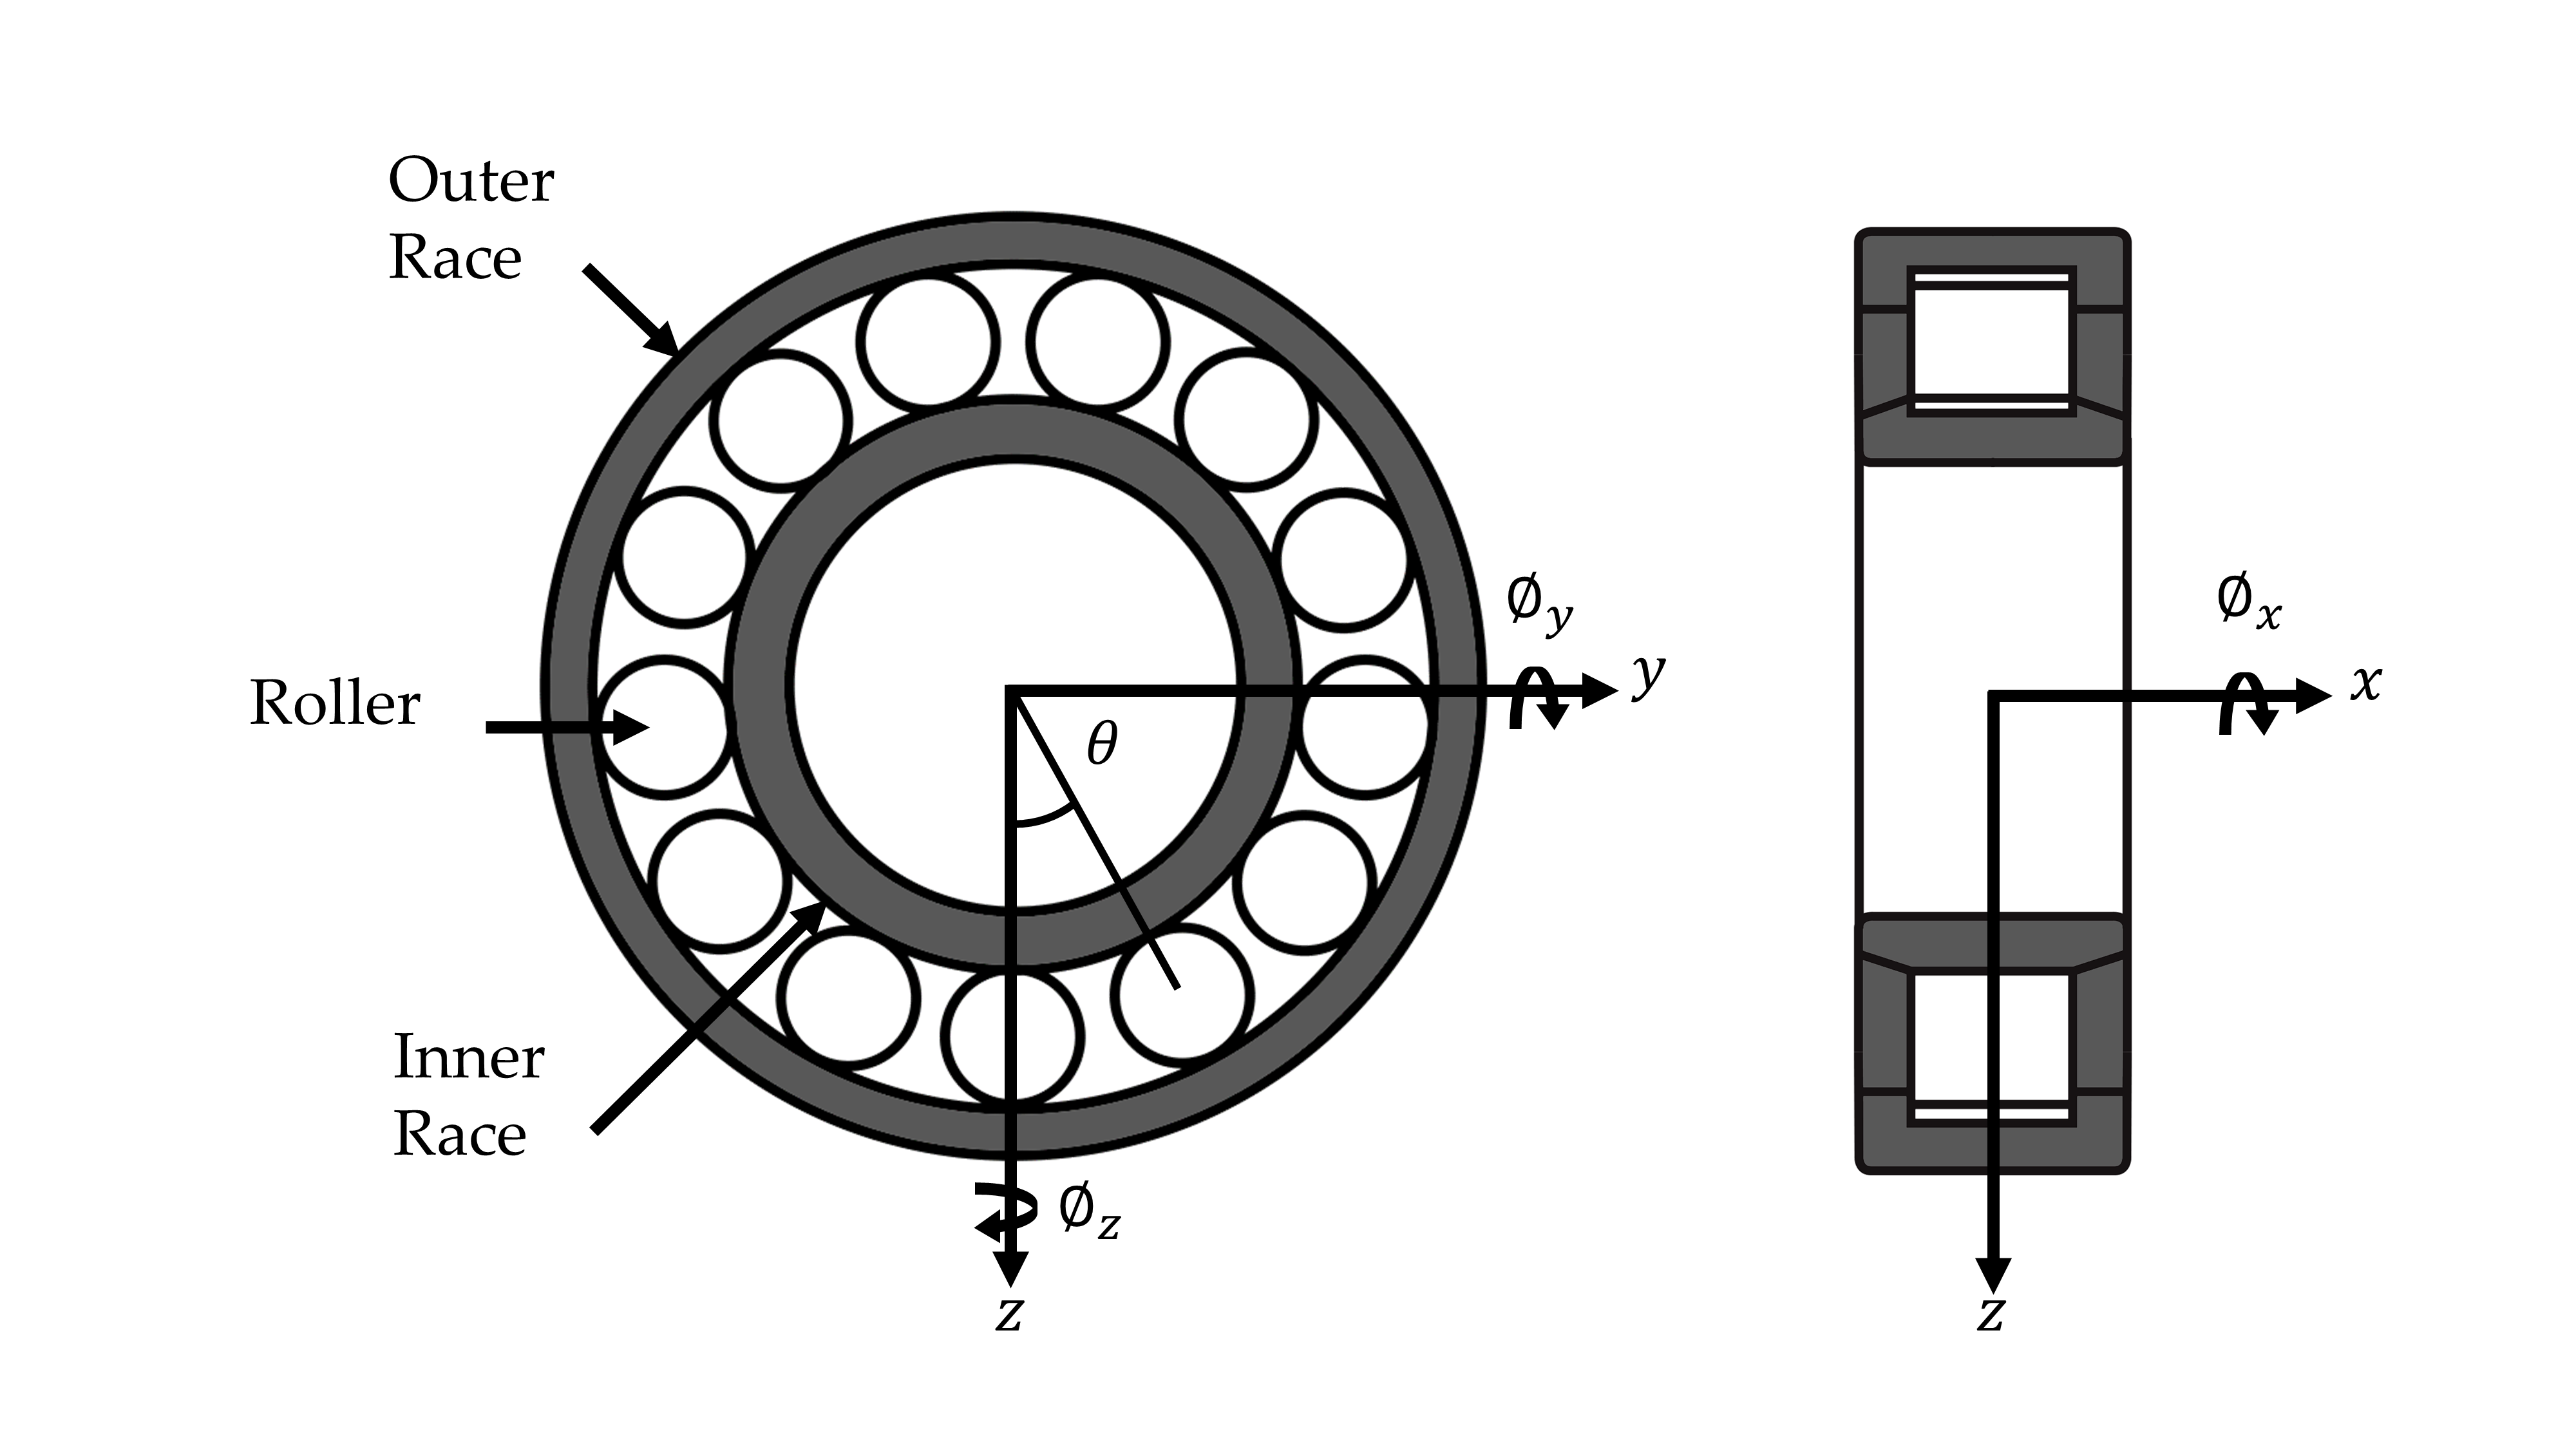
\includegraphics[width=150mm]{FlexiTribo Figure 3. Bearing Schematic.png}
	\caption{Bearing schematic.}
	\label{Bearing schematic}
\end{figure} 

Between the roller and raceways, under sufficient load, the pressures in the non-conformal contact are high enough to cause elastic deformation of the surfaces and a significant increase in lubricant viscosity. This, combined with relative motion between contacting bodies, leads to the generation of an EHL contact. The stiffness of the EHL film is typically 1-2 orders greater than the stiffness of the contacting bodies \cite{Dietl1997}. In this analysis, the film stiffness was calculated using:

\begin{equation}\label{Film stiffness}
	K_{E H L}=\frac{d w}{d h_c}
\end{equation}

The lowest average film stiffness was $5.1 \times 10^9 \mathrm{~N} / \mathrm{m}$, which is over one order greater than the contacting material stiffness. The material therefore dominates the stiffness of the contact, and the stiffness of the EHL film can be neglected. The film is modelled as a rigid element that is present between the roller and race \cite{Walford1983} \cite{Dareing1975} \cite{Mehdigoli1990}.

The contact deformation $(\delta)$ is therefore a function of the displacement of the inner bearing race, angular displacement of the roller about the rotationall axis $(\theta)$ thickness of the EHL film $\left(h_c\right)$ and any clearance or radial preload $( \pm C)$ within the bearing \cite{Rahnejat1985} \cite{Mohammadpour2015c}:

\begin{equation}\label{Contact deformation flextribo}
	2 \delta=2\left(h_c-C\right)+z \cos (\theta)+y \sin (\theta)
\end{equation}

Figure \ref{Dry vs lubricated roller-race contact} demonstrates this more clearly. The total contact deformation is the summation of the central film thickness $\left(h_c\right)$ and the material deformation $\left(\delta_m\right)$ predicted from the dry-Hertzian contact assumption. Conventional dry analysis only accounts for the dry material deformation at the contact.

\begin{figure}  
	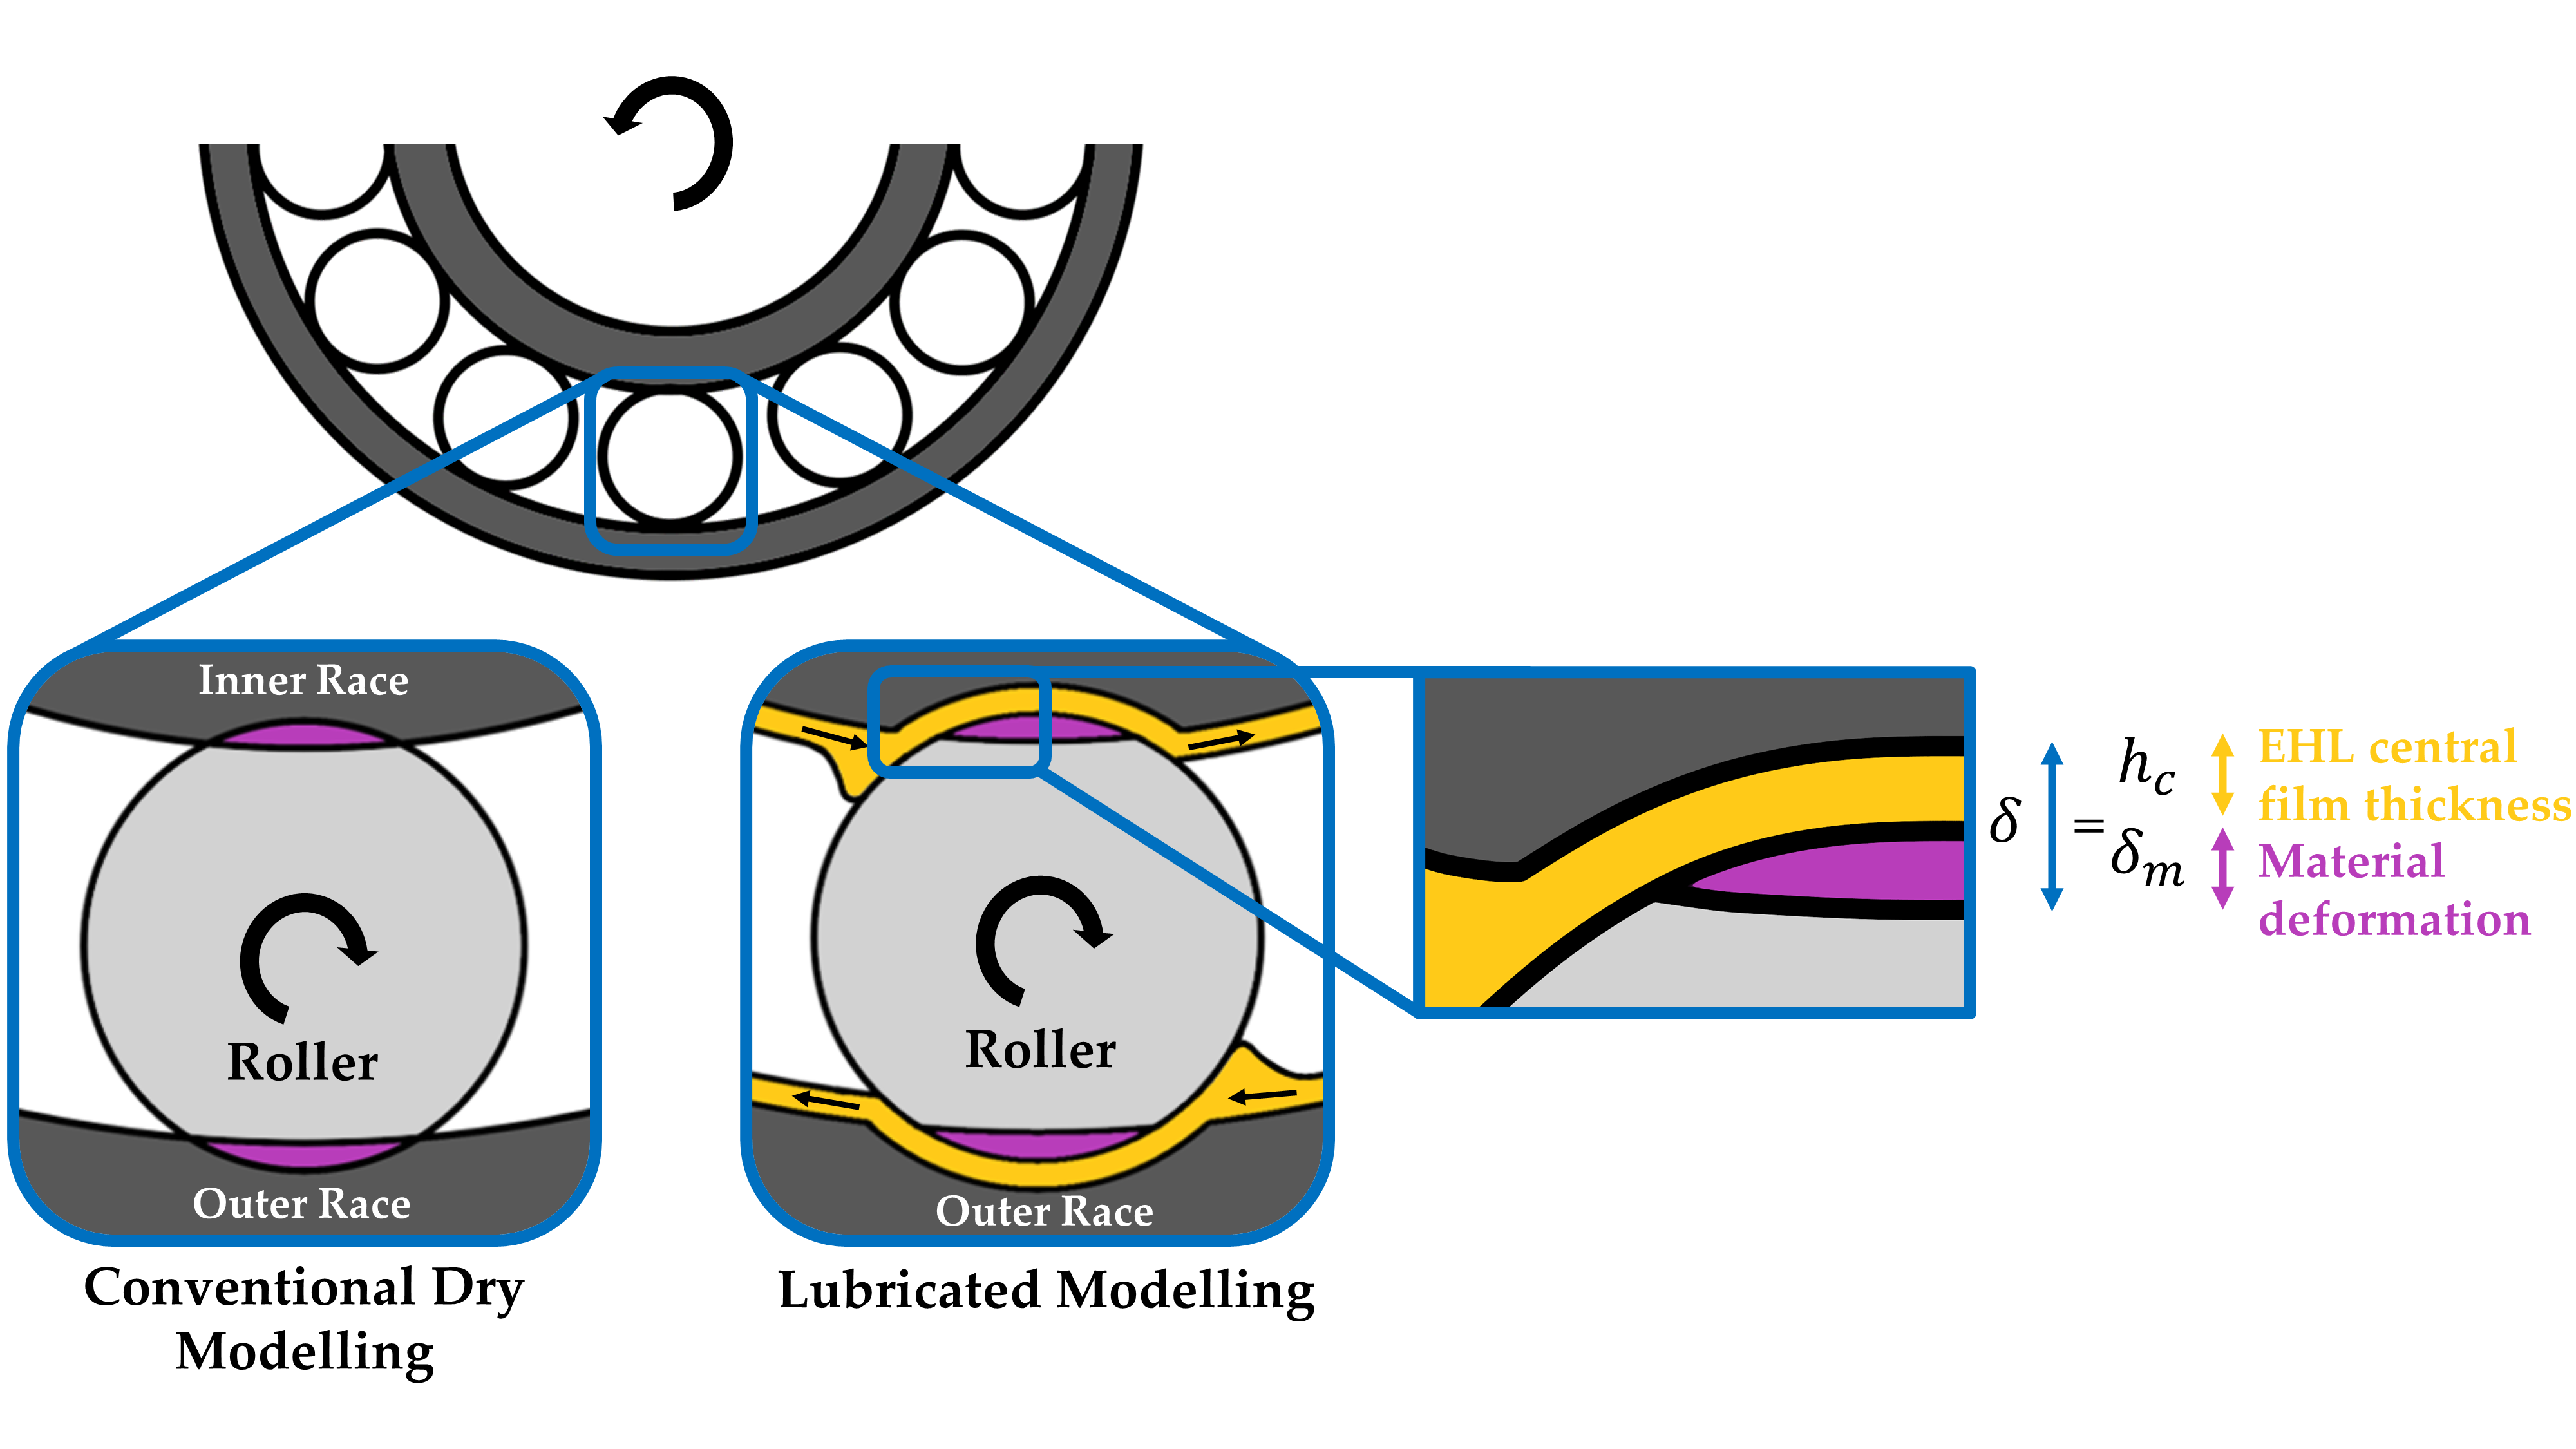
\includegraphics[width=150mm]{FlexiTribo Figure 4. Dry vs Lubricated Roller-Race Contact.png}
	\caption{Dry vs lubricated roller-race contact.}
	\label{Dry vs lubricated roller-race contact}
\end{figure} 

The extrapolated central film thickness for a line contact, assuming a fully flooded contact inlet, is therefore obtained from \cite{Dowson1979}: 

\begin{equation}\label{DowsonToyodaCentralFilm}
	h_c=R_r\left[3.06 G^{* 0.56} U^{* 0.69} W^{*-0.1}\right]
\end{equation}

where the following dimensionless parameters are used:

\begin{equation}\label{DowsonToyodaDimensionless}
	W^*=\frac{W}{E_r R_r l_a}, U^*=\frac{\eta_0 U}{E_r R_r}, G^*=E_r \alpha
\end{equation}

Comprehensive analytical models \cite{Nelias2008} \cite{Majdoub2020} account for the tilting and skew of the rolling elements. Skew has the effect of varying the entrainment speed along the length of the roller, and tilt will affect the contact gap. Due to the stiff housing and shaft used in this analysis, the tilt and skew angles are very small. The entraining motion and contact gap along the contact length can be considered consistent, and a 1-dimensional analysis for EHL film thickness is therefore appropriate \cite{Gupta1979}.

The bearings are modelled with light preload due to mounting interference. In practical applications, preload is applied to prevent skidding and chaotic behaviour due to the emergence of zero stiffness regions \cite{Mevel1993}. In contrast, excessive preload can lead to frictional power loss and wear. Assuming pure rolling, the speed of entraining motion is given by \cite{Spikes2015} \cite{Shi2015}: 
	
\begin{equation}\label{SpikesEntrainmentSpeed}
	u=\frac{R \omega}{r}\left(\frac{(R+2 r)}{(R+r)}\right)
\end{equation}

Due to the dependency of load on film thickness, an iterative approach is performed to calculate the contact force. Convergence criteria for the EHL film must be met at each time step of the simulation before the bearing forces are returned to the system level model and the equations of motion are solved:

\begin{equation}\label{FilmConvergence}
	\frac{h_c^m-h_c^{m-1}}{h_c^{m-1}} \leq 0.001
\end{equation}

where $m$ represents the iteration number.

Individual roller-race contact forces are calculated based on the contact deformation. In the case of a rolling element, a cylindrical body of finite length, the contact problem is non-Hertzian. The surfaces cannot be modelled as locally quadratic due to the presence of crowned (rounded) edges \cite{Singh1974}. The most widely used technique to calculate the force-deflection relationship is the contact slicing technique. Whilst this does not reflect edge stress concentrations, these stresses are only distributed over a small area and hence can be neglected for the purpose of force equilibrium \cite{Harris2007a}. In general, this technique is favoured for its simplicity, speed, and sufficient accuracy. The contact slicing technique employed in this study was developed by Andreason \cite{Andreason1973} for modelling these non-Hertzian line contacts.
 
Modelling the roller-race contacts as a line contact between a cylindrical roller and a flat surface, Lundberg’s \cite{Lundberg1949} expression between contact force per unit length ($w$) and deformation ($\delta$) was used. 

\begin{equation}\label{Lundberg deflection}
	\frac{\delta}{l_a}=\frac{2 w}{\pi E_r l_a} \ln \frac{\pi E_r l_a}{w}
\end{equation}

where $E_r$ is the equivalent elastic modulus of the two materials and $l_a$ is the active length of the roller. This assumes that the pressure distribution is uniform along the length of the contact, and elliptical across it. This neglects side leakage along the contact $\left(x_c\right)$ due to the contact dimensions in this direction being much larger than dimensions across it $\left(y_c\right)$. This is valid apart from the small regions at the edges of the contact.

From Equation \ref{Lundberg deflection}, contact forces per unit length of an individual slice along the roller-race contact can be calculated. This is valid if there is no separation of the bodies, i.e., the contact deformation does not become negative $\left(\delta_k>0\right)$.

\begin{equation}\label{Contact force per unit length Lundberg}
	w_s=\pi E_r l_s\left(\frac{0.5 \delta_s}{7.358 l_s}\right)^{1.11}
\end{equation}

where $s$ represents the slice number, and $l$ represents the slice length.

The application of the slicing technique was validated against open literature. de Mul et al. \cite{DeMul1989_2} compared results obtained from an experimental rig with numerical results calculated using both the approximate slicing technique and the sophisticated non-Hertzian technique \cite{DeMul1986}. By replicating the geometry of the test bearing used in their analysis, the application of Andreason’s slicing technique used for this analysis was validated with good agreement (see Figure \ref{Contact level validation}). This method is a much faster way of calculating contact load and moment than more sophisticated methods by de Mul, yet still maintains high accuracy.

\begin{figure}  
	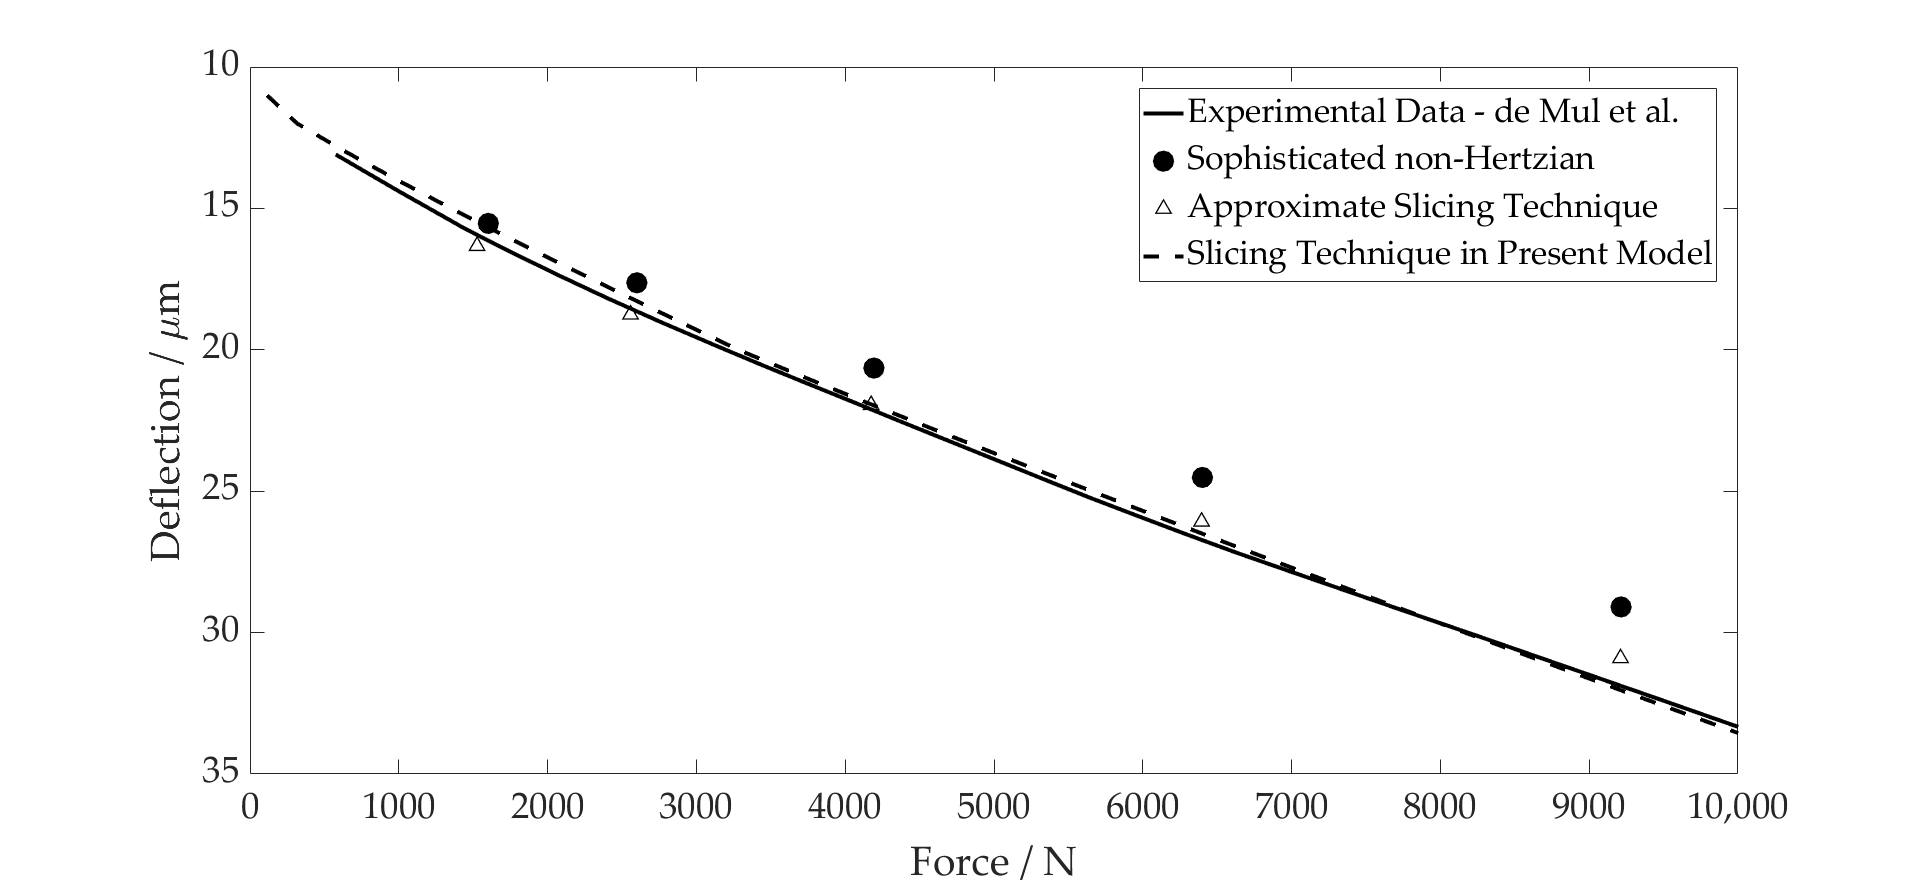
\includegraphics[width=150mm]{FlexiTribo Figure 5. Contact Level Validation.png}
	\caption{Contact level validation.}
	\label{Contact level validation}
\end{figure} 

The total contact load $W$ and moment $T$ are obtained by summing the contributions from all loaded slices:

\begin{equation}\label{Total contact load flexitribo}
	W=\sum_s w_s l_s
\end{equation}

\begin{equation}\label{Total contact torque flexitribo}
	T=\sum_s w_s l_s x_{c, s}
\end{equation}

with $x_{c, s}$ being the distance to the centre of each slice in the conjunction coordinate system. It is assumed that total contact deflection is shared equally between the inner and outer races despite slight differences in contact geometry. The entrainment velocity is equal at each contact, which is the governing parameter for the lubricated contact force differences.

Experimental measurements show that the damping of a rolling element bearing arises from multiple sources \cite{Dietl1997}, including:
 
\begin{enumerate}
	\item Lubricant film damping at the contacts.
	\item Material damping due to Hertzian deformations.
	\item Interface damping between assembled components
\end{enumerate}

These measurements show that damping decreases with rotational speed, tending towards a constant value. Sopanen and Mikkola \cite{Sopanen2003_1} summarize the findings of Mitsuya et al. \cite{Mitsuya1992} and Aini et al. \cite{Aini2002}, concluding that the film damping is moderate. The linearized viscous damping method adopted in their study is therefore also adopted here. The damping force for each roller is obtained as a factor of the contact stiffness and contact penetration velocity \cite{Kramer1993}. This is defined as:

\begin{equation}\label{Kramer damping}
	\left|F_d\right|=-f_{\text {damp }} K_c \dot{q}
\end{equation}

where $K_c$ is the contact stiffness, and the damping factor, $f_{\text {damp}}$, is in the range of $(0.25-2.5) \times 10^{-5}$ as reported by \cite{Kramer1993}.

At each time step of the analysis, these calculations are performed for each individual roller in the complement. The total bearing force acting on the inner race is solved by splitting the total contact force on each roller into its components and summing their contributions.

\begin{equation}\label{Total bearing force z flexitribo}
	f_{z, i}^*=\sum_N W \cos (\theta)-\sum_N F_d \cos (\theta)
\end{equation}

\begin{equation}\label{Total bearing force y flexitribo}
	f_{y, i}^*=\sum_N W \sin (\theta)-\sum_N F_d \sin (\theta)
\end{equation}

Due to the bearing preload, contact is maintained throughout the rollers’ orbit; hence no emerging clearances are modelled in the lubricated analysis. The contact separation is also unaffected by rolling element centrifugal forces, which are negligible when compared to the contribution of the dynamic load and the EHL film in this study. These have therefore been neglected.

Surface measurements of the rollers used in this analysis were taken using an Alicona InfiniteFocus Variation Microscope. The composite surface roughness value of a roller and inner race was calculated to be 91.3 nm. This gives a lambda value of 5.88 for the thinnest EHL film at 1000 rpm. Asperity interaction is not considered as the EHL film fully supports the load. Due to the pure rolling and zero sliding assumption, friction at the contacts is therefore neglected and the analysis is performed under isothermal conditions. 

The bearing geometry is detailed in Table \ref{Cylindrical Roller Bearing Specification}. Rheological and material properties are detailed in Table \ref{Bearing Rheological Properties}, representing ambient operating conditions in an individual hub-motor transmission. 

\begin{table*}
	%\captionsetup{justification=centering}
	\caption{Cylindrical Roller Bearing Specification}
	\label{Cylindrical Roller Bearing Specification}
	\centering
	\renewcommand{\arraystretch}{1.5}%
	\begin{tabular}{|c|c|}
		\hline
		\ \textbf{Parameter} & \textbf{Value} \\ [0.5ex]
		\hline
		Inner race bore diameter & 25 $mm$ \\ [0.5ex]
		\hline
		Pitch diameter & 60 $mm$ \\ [0.5ex]
		\hline
		Roller diameter & 8.8 $mm$ \\ [0.5ex]
		\hline
	    Roller length & 15 $mm$ \\ [0.5ex]
		\hline
	    Number of rollers & 17 \\ [0.5ex]
		\hline
		Radial interference & 2 $\mu \mathrm{m}$ \\ [0.5ex]
		\hline
	\end{tabular}
\end{table*}

\begin{table*}
	%\captionsetup{justification=centering}
	\caption{Bearing Rheological Properties}
	\label{Bearing Rheological Properties}
	\centering
	\renewcommand{\arraystretch}{1.5}%
	\begin{tabular}{|c|c|}
		\hline
		\ \textbf{Parameter} & \textbf{Value} \\ [0.5ex]
		\hline
		Pressure Viscosity Coefficient ($\alpha$) & 2.1 $\times 10^{-8}\mathrm{~Pa}^{-1}$ \\ [0.5ex]
		\hline
		Atmospheric lubricant dynamic viscosity & 0.08 Pa.s \\ [0.5ex]
		\hline
		Lubricant inlet density ($\rho_0$) & 833.8 $\mathrm{~kg}\cdot\mathrm{m}^{-3}$ \\ [0.5ex]
		\hline
		Modulus of elasticity of contacting solids & 210 GPa \\ [0.5ex]
		\hline
	    Poisson’s ratio of contacting solids & 0.3 \\ [0.5ex]
		\hline
	\end{tabular}
\end{table*}

\subsection{Representative Excitation Methodology}

The system level model is decomposed, with excitation forces calculated externally before application within the model. A separate electrified transmission model is used to generate realistic excitation forces and torques from a spur gear pair and a permanent magnetic synchronous motor (PMSM). This system represents the first stage of an electric hub motor used in automotive applications. 

Radial and tangential gear pair forces at the pinion centre, as well as torque fluctuations of the electric motor are extracted to be used as inputs to the system level model. These are applied as external forces to the shaft, $f^a$, from Equation \ref{External forces}. All bodies in this separate system were modelled as rigid, so that structural excitation forces did not contribute to the resultant forces at the pinion.

The motor has a peak torque of 68~$\mathrm{Nm}$, and a maximum operating speed of 21~000~$\mathrm{rpm}$. The torque transfer through the gear pair reduces as the speed increases due to the torque profile of the PMSM, as shown in Figure \ref{PMSM torque profile}. Stator tooth forces from the PMSM are neglected in the model due to their minimal contribution to lateral forces once resolved. For input to the model, the radial and normal forces are simplified by adopting sinusoidal inputs of the same magnitude and frequency of the gear pair at different speeds. The torque ripple from the motor is simplified using the same method.

\begin{figure}  
	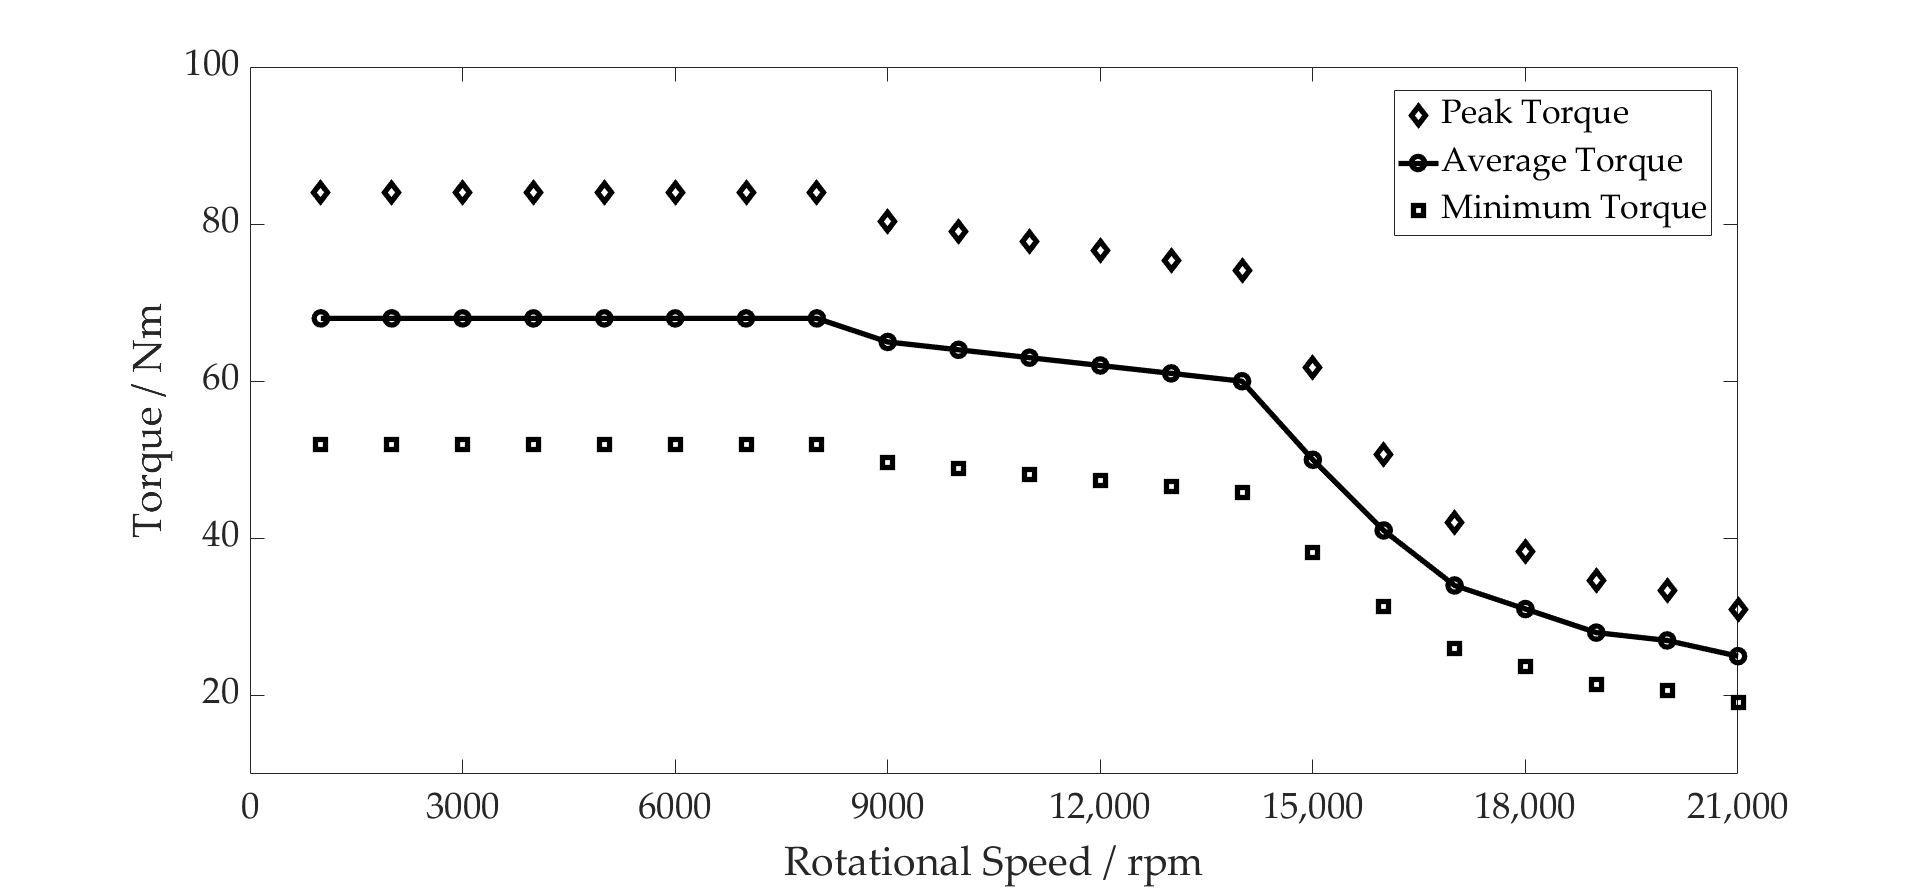
\includegraphics[width=150mm]{FlexiTribo Figure 6. PMSM Torque Profile and Maximum and Minimum Torque Fluctuation.png}
	\caption{PMSM torque profile and maximum and minimum torque fluctuation.}
	\label{PMSM torque profile}
\end{figure} 

\begin{table*}
	%\captionsetup{justification=centering}
	\caption{Pinion Geometry}
	\label{Pinion Geometry}
	\centering
	\renewcommand{\arraystretch}{1.5}%
	\begin{tabular}{|c|c|}
		\hline
		\ \textbf{Parameter} & \textbf{Value} \\ [0.5ex]
		\hline
		Number of teeth 17 & \\ [0.5ex]
		\hline
		Normal module & 0.004 $m$ \\ [0.5ex]
		\hline
		Normal pressure angle & 20 $^{\circ}$ \\ [0.5ex]
		\hline
		Helix angle at pitch circle & 0 $^{\circ}$ \\ [0.5ex]
		\hline
		Active tip diameter & 0.076 $m$ \\ [0.5ex]
		\hline
		Active root diameter & 0.065 $m$ \\ [0.5ex]
		\hline
	    Width & 0.035 $m$ \\ [0.5ex]
		\hline
	\end{tabular}
\end{table*}

\begin{table*}
	%\captionsetup{justification=centering}
	\caption{Gear Geometry}
	\label{Gear Geometry}
	\centering
	\renewcommand{\arraystretch}{1.5}%
	\begin{tabular}{|c|c|}
		\hline
		\ \textbf{Parameter} & \textbf{Value} \\ [0.5ex]
		\hline
		Number of teeth & 51 \\ [0.5ex]
		\hline
		Normal module & 0.004 $m$ \\ [0.5ex]
		\hline
		Normal pressure angle & 20 $^{\circ}$ \\ [0.5ex]
		\hline
		Helix angle at pitch circle & 0 $^{\circ}$ \\ [0.5ex]
		\hline
		Active tip diameter & 0.212 $m$ \\ [0.5ex]
		\hline
		Active root diameter & 0.202 $m$ \\ [0.5ex]
		\hline
		Width & 0.030 $m$ \\ [0.5ex]
		\hline
	\end{tabular}
\end{table*}

\section{Results and Discussion}

A quasi-dynamic speed sweep has been performed from 1000 to 21~000~$rpm$. The simulations are performed every 1000~$rpm$, refined to 250~$rpm$ intervals throughout a period of system resonance between 12~000~$rpm$ and 14~000~$rpm$. The operating envelopes are generated by plotting the maximum and minimum values from the steady-state signals at each speed interval. The conjunction level results are obtained from an individual roller and its contact with the inner raceway. The component and system level results are taken from the geometric centre of the inner bearing race, corresponding to the bearing seat on the shaft. The following figures represent results in the $y$-direction, the largest component of excitation due to the tangential force from the gear meshing.

The contact level results (Figure \ref{Rolling element contact stiffness - Dry vs lubricated maximum values}) show a difference in the contact stiffness between the dry and lubricated models. The dry model follows the torque profile of the motor, with stiffness decreasing as the contact forces reduce. The period of resonance leads to the larger amplitude excitation of the shaft, resulting in an increase in the contact stiffness due to the force–deflection non-linearity. The lubricated model, however, shows an increase in the contact stiffness throughout the speed sweep. This is due to the higher levels of deformation at the contact as the lubricant is entrained, which increases with the shaft rotational velocity. This behaviour was experimentally observed by Dietl, concluding that the oil-wedge between the rolling elements and raceways reduces the internal clearance of the bearing and increases its stiffness \cite{Dietl1997}. The contact stiffness in the lubricated bearing model under the same operating conditions is therefore 24.9\% greater at 21~000~$rpm$.

\begin{figure}  
	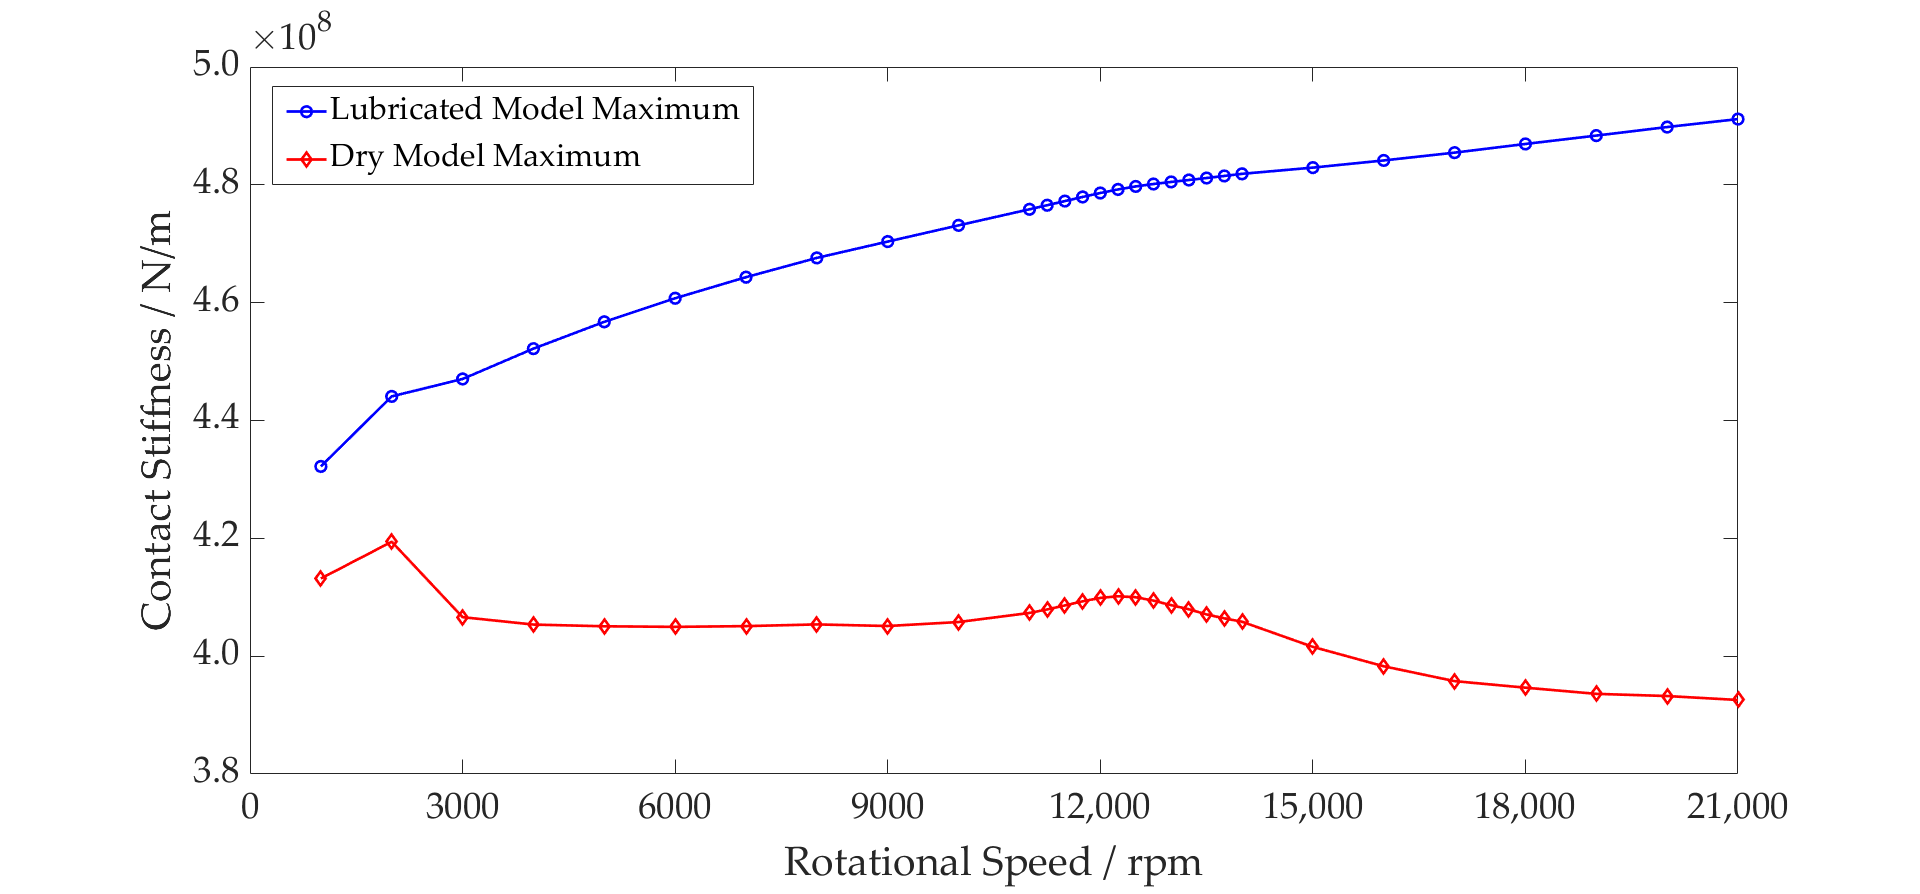
\includegraphics[width=150mm]{FlexiTribo Figure 7. Rolling Element Contact Stiffness - Dry vs Lubricated Maximum Values.png}
	\caption{Rolling element contact stiffness - Dry vs lubricated maximum values.}
	\label{Rolling element contact stiffness - Dry vs lubricated maximum values}
\end{figure} 

The peak contact force has been compared between both models. The percentage increase between the dry and lubricated models is shown in Figure 	\ref{Rolling element contact force - Dry vs lubricated percentage increase}. This more clearly shows the disparity between both models at the contact, with the largest difference being 9.6 times at maximum speed. During resonance, the inner race force reaches a peak of 1514~$\mathrm{N}$, resulting in surface deformation magnitudes of 0.92~$\mu \mathrm{m}$ and 3.81~$\mu \mathrm{m}$ at the dry and lubricated conjunctions, respectively. As noted in previous works [15], higher loads lead to a greater surface deformation to the film thickness ratio, causing the percentage difference between the dry and lubricated models to reduce. Once the loads reduce as the speed increases, the percentage increase continues to rise.

\begin{figure}  
	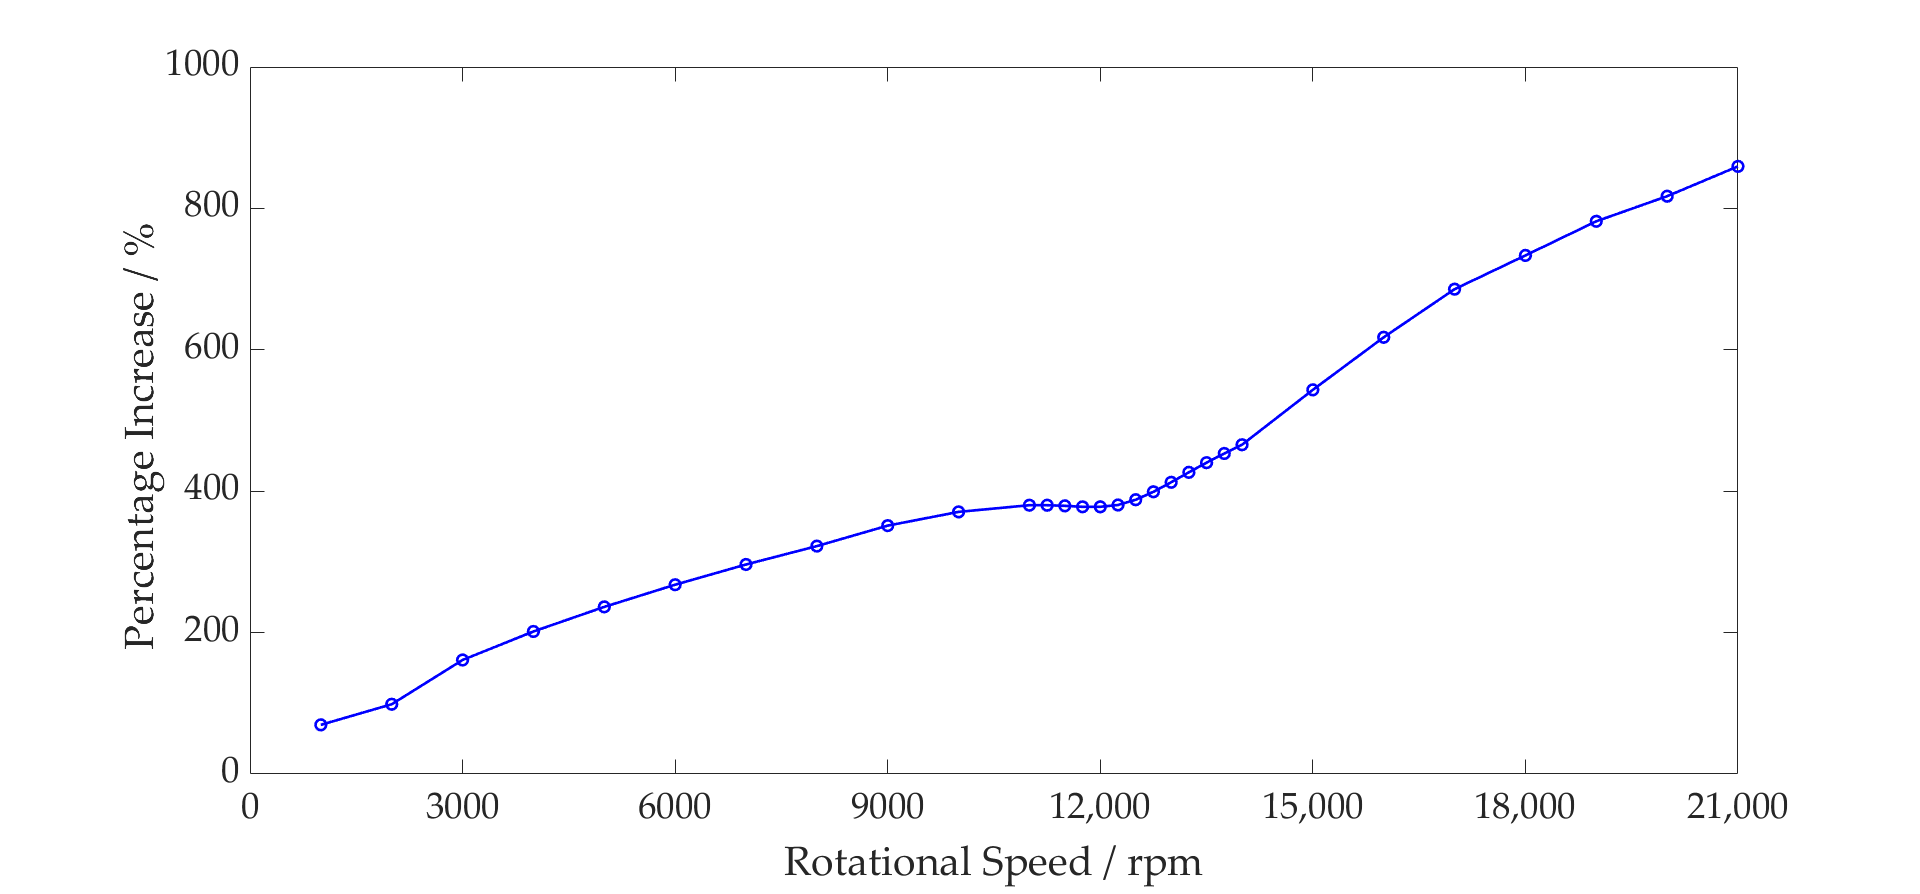
\includegraphics[width=150mm]{FlexiTribo Figure 8. Rolling Element Contact Force - Dry vs Lubricated Percentage Increase.png}
	\caption{Rolling element contact force - Dry vs lubricated percentage increase.}
	\label{Rolling element contact force - Dry vs lubricated percentage increase}
\end{figure} 

The total bearing stiffness is a combination of all contact stiffnesses between the elements and raceways. These contact stiffnesses vary non-linearly with force, resulting in the total bearing stiffness varying accordingly. For the dry model, this is clearly demonstrated, with the greater total bearing stiffness at the peak of the resonance due to the greater bearing forces (see Figure \ref{Inner race stiffness - Dry vs lubricated operating envelope}). This does not, however, capture the change of the total bearing stiffness with speed; the average bearing stiffness does not change. The lubricated bearing is not only stiffer than the dry bearing, but this stiffness also increases with speed. This is shown in Figure \ref{Inner race stiffness - Dry vs lubricated operating envelope} by the non-linear increase in the average lubricated bearing stiffness values compared to the constant values for the dry model. The combination of these two factors leads to the lubricated model having a $16.6 \%$ greater maximum total bearing stiffness at 21~000~$\mathrm{rpm}$ than the dry model.

\begin{figure}  
	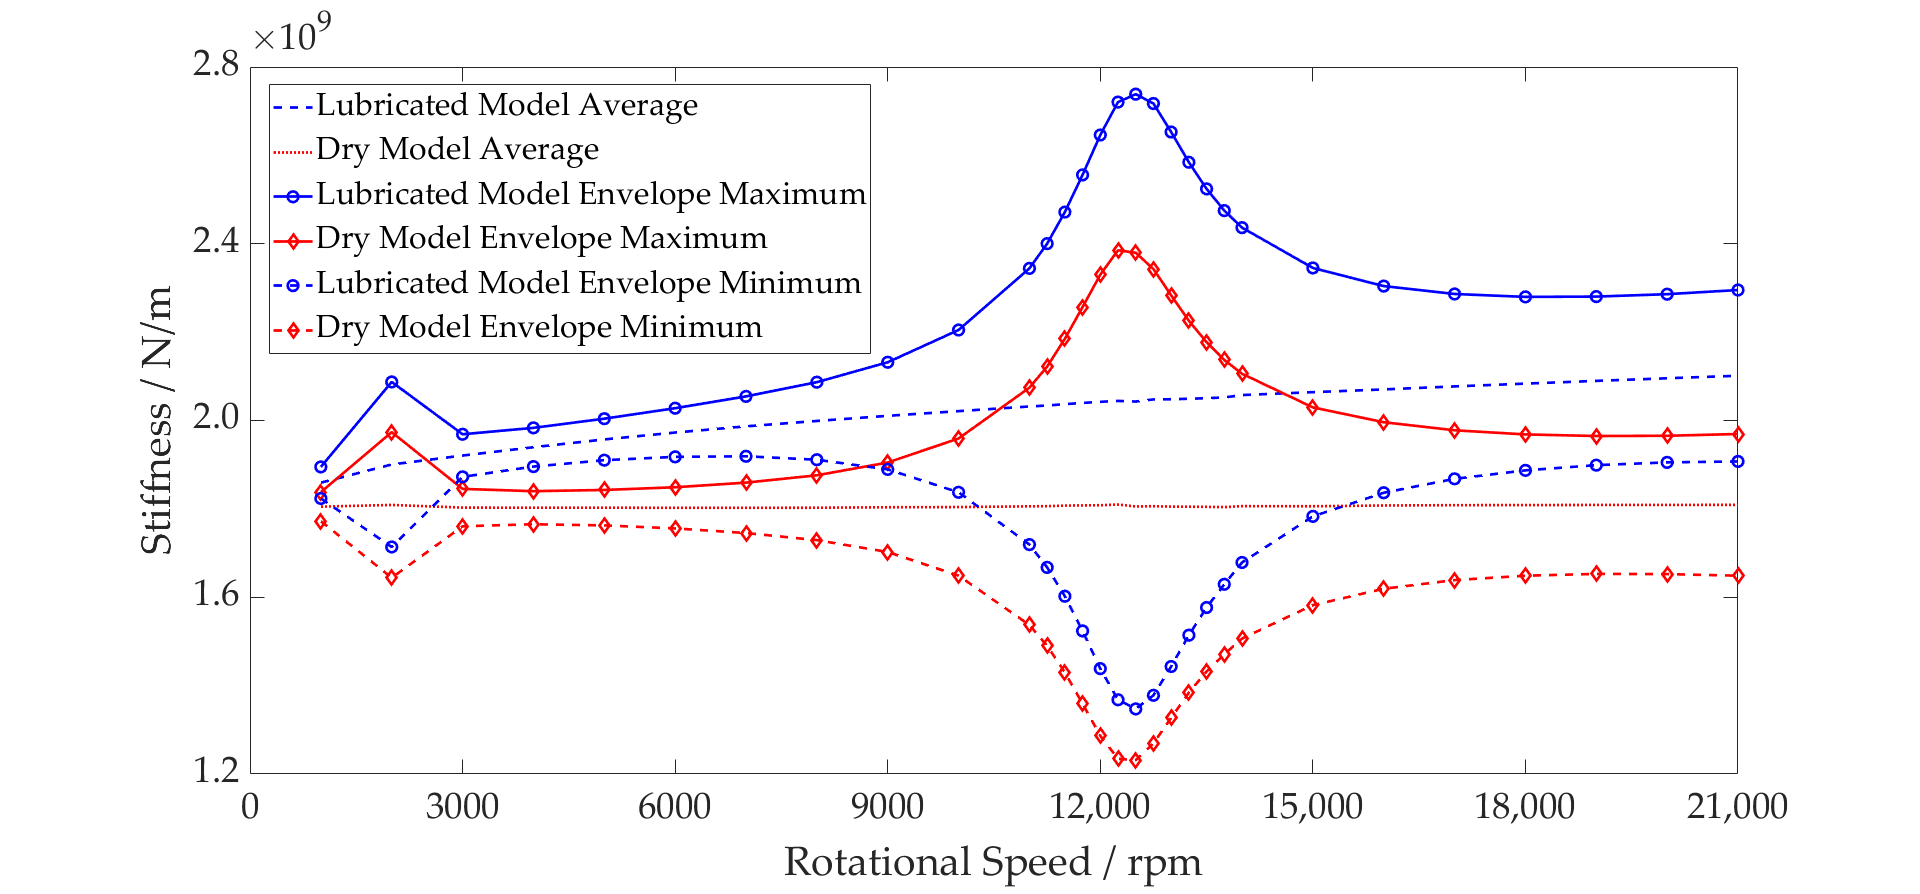
\includegraphics[width=150mm]{FlexiTribo Figure 9. Inner Race Stiffness - Dry vs Lubricated Operating Envelope.png}
	\caption{Inner race stiffness - Dry vs lubricated operating envelope.}
	\label{Inner race stiffness - Dry vs lubricated operating envelope}
\end{figure} 

Due to the greater total stiffness of the bearing, the shaft displacement of the lubricated model is lower both on average and peak to peak for the same applied force in comparison to the dry model (see Figure \ref{Inner race displacement - Dry vs lubricated operating envelope}). Through the period of resonance, the large inner race forces result in the roller–race separation of the unloaded rollers within the dry model. This leads to greater shaft displacement as the inner race moves into this region of zero stiffness until roller–race contact is mademade, and a reaction force is established.

\begin{figure}  
	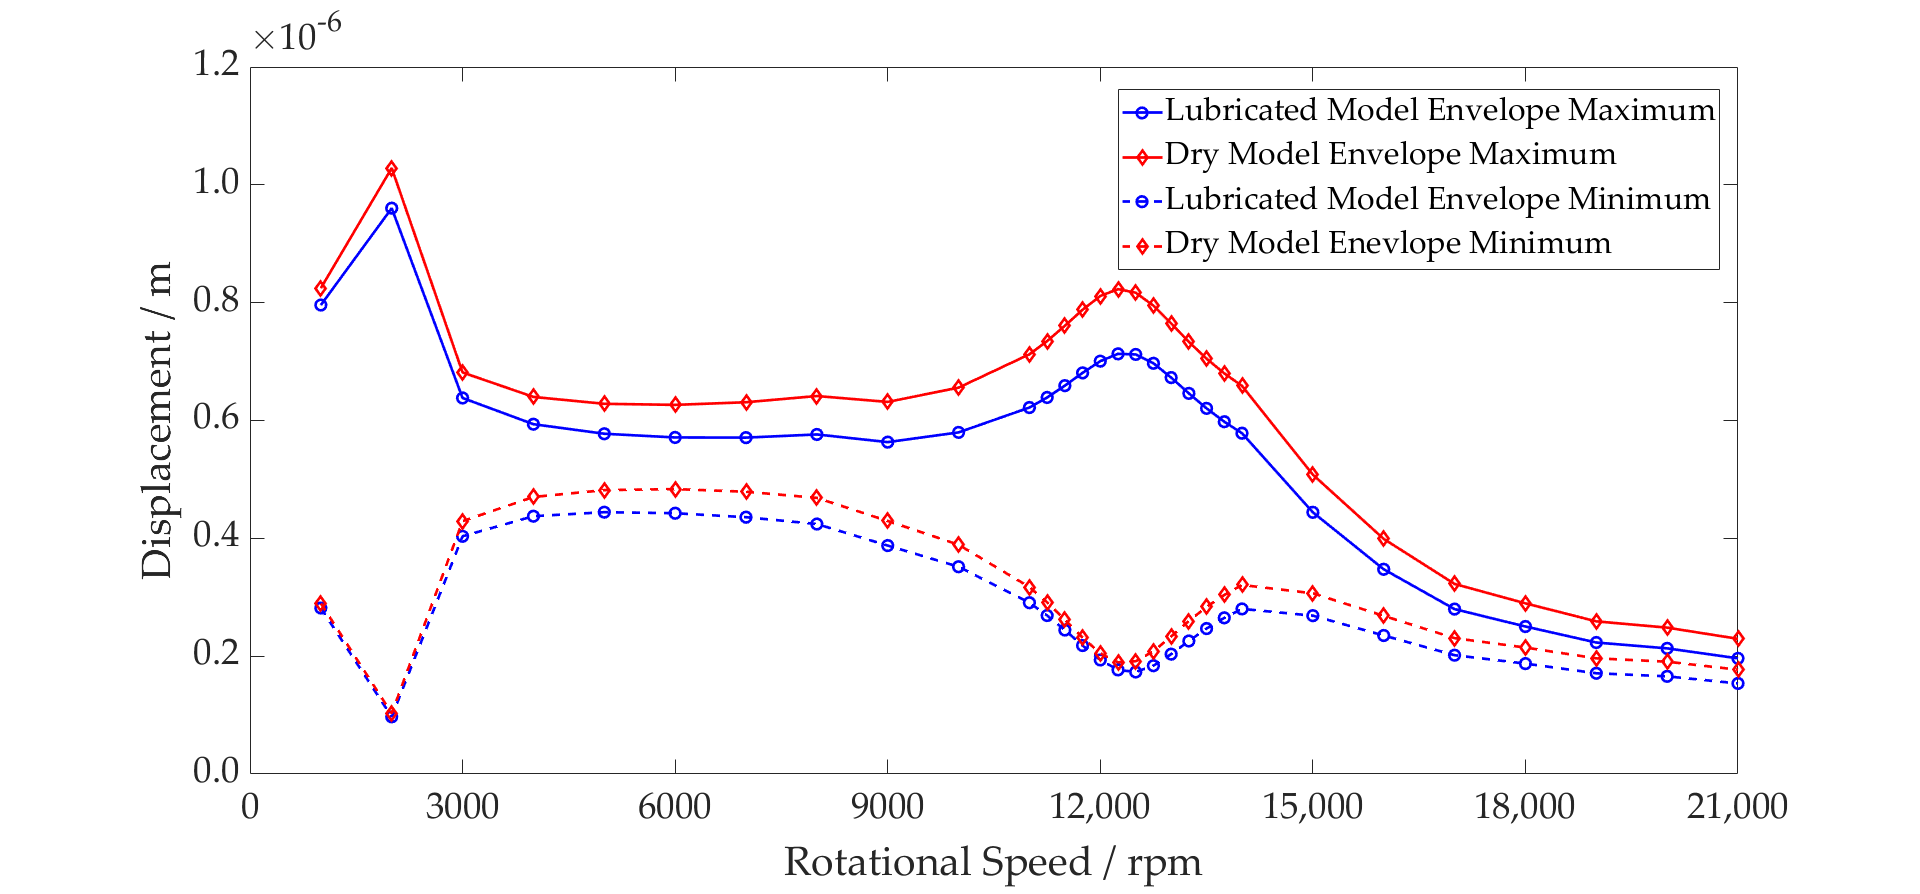
\includegraphics[width=150mm]{FlexiTribo Figure 10. Inner Race Displacement - Dry vs Lubricated Operating Envelope.png}
	\caption{Inner race displacement - Dry vs lubricated operating envelope.}
	\label{Inner race displacement - Dry vs lubricated operating envelope}
\end{figure} 

Figure \ref{Inner race acceleration - Dry vs lubricated operating envelope} shows that the acceleration peak of the system resonance occurs at 12~500~$\mathrm{rpm}$ (3542~0$\mathrm{Hz}$) for the lubricated model as opposed to 12~250~$\mathrm{rpm}$ (3470~$\mathrm{Hz}$) for the dry model. This shift in natural frequency indicates a stiffer overall system. The magnitude difference between the dry and lubricated models can also be attributed to the unloaded regions of the dry bearing. The contact deformation arising from the loading of the inner race is sufficient to cause the rollers geometrically opposite to become separated from their contacts. Contact is lost between the roller and raceway, leading to zero contact stiffness. The inner race moves into this region until it is reacted by a contact force once again. These regions of zero stiffness are shown in Figure \ref{Rolling element contact stiffness - Dry vs lubricated minimum values}, where the minimum stiffness of an individual rolling element and raceway contact in the dry model drops to zero due to separation. For the lubricated model, contact is maintained throughout.

\begin{figure}  
	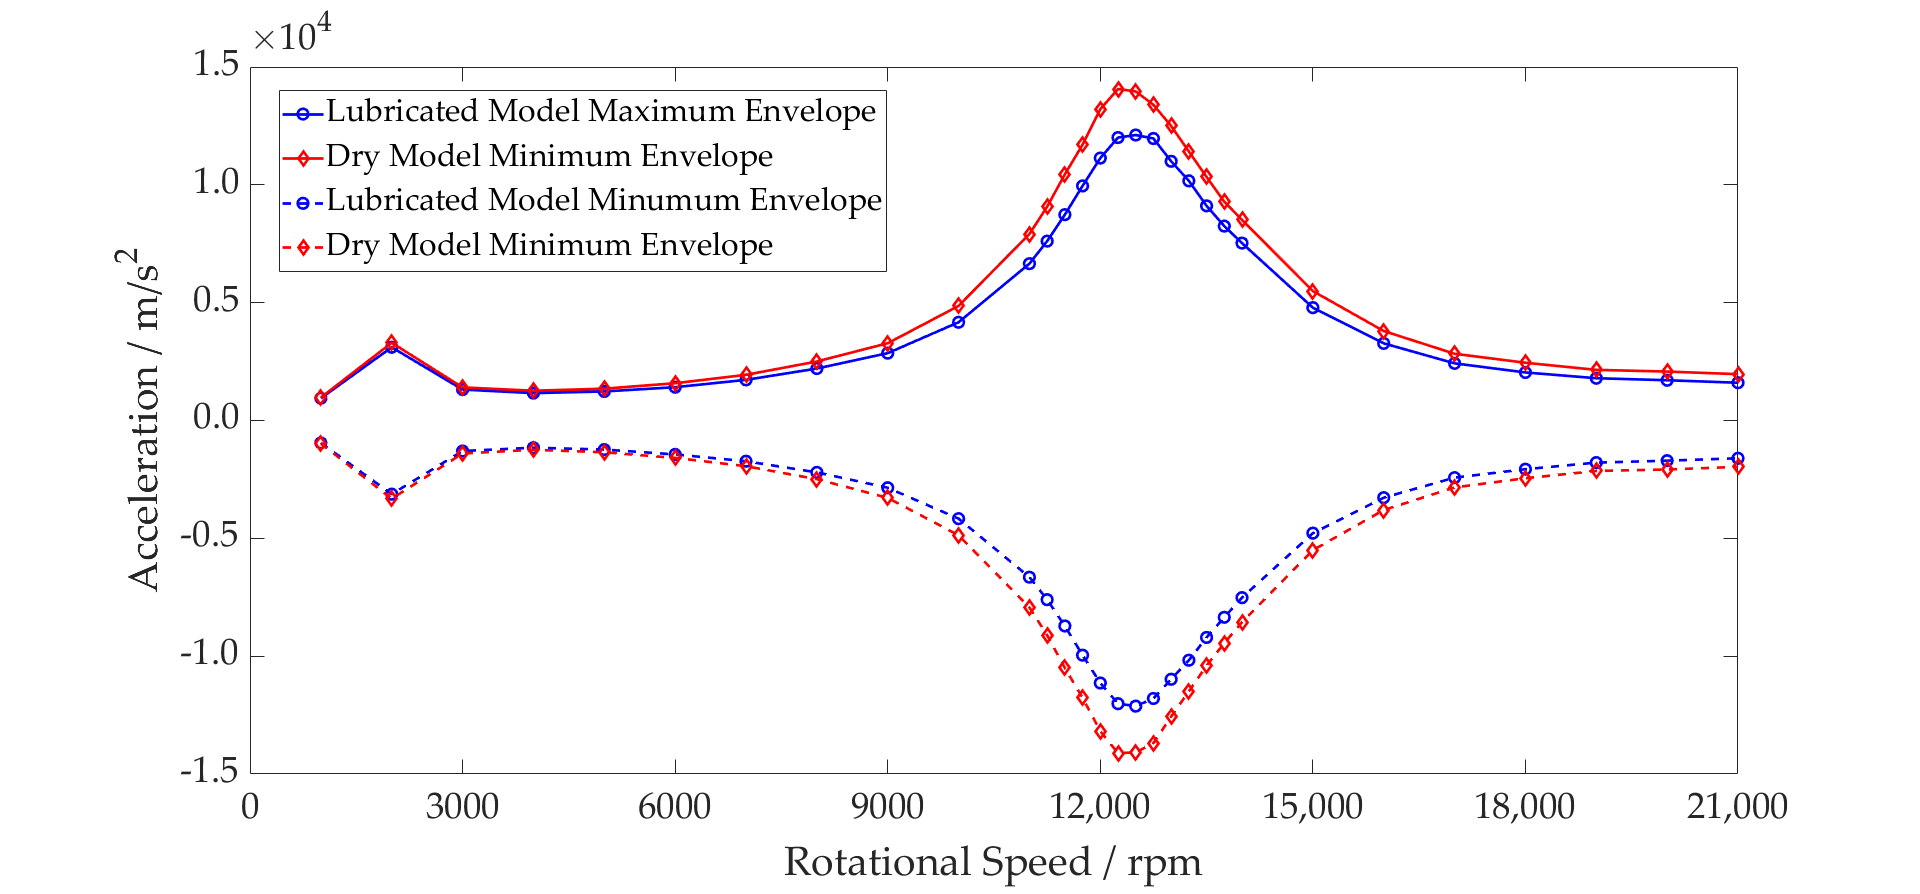
\includegraphics[width=150mm]{FlexiTribo Figure 11. Inner Race Acceleration - Dry vs Lubricated Operating Envelope.png}
	\caption{Inner race acceleration - Dry vs lubricated operating envelope.}
	\label{Inner race acceleration - Dry vs lubricated operating envelope}
\end{figure}

\begin{figure}  
	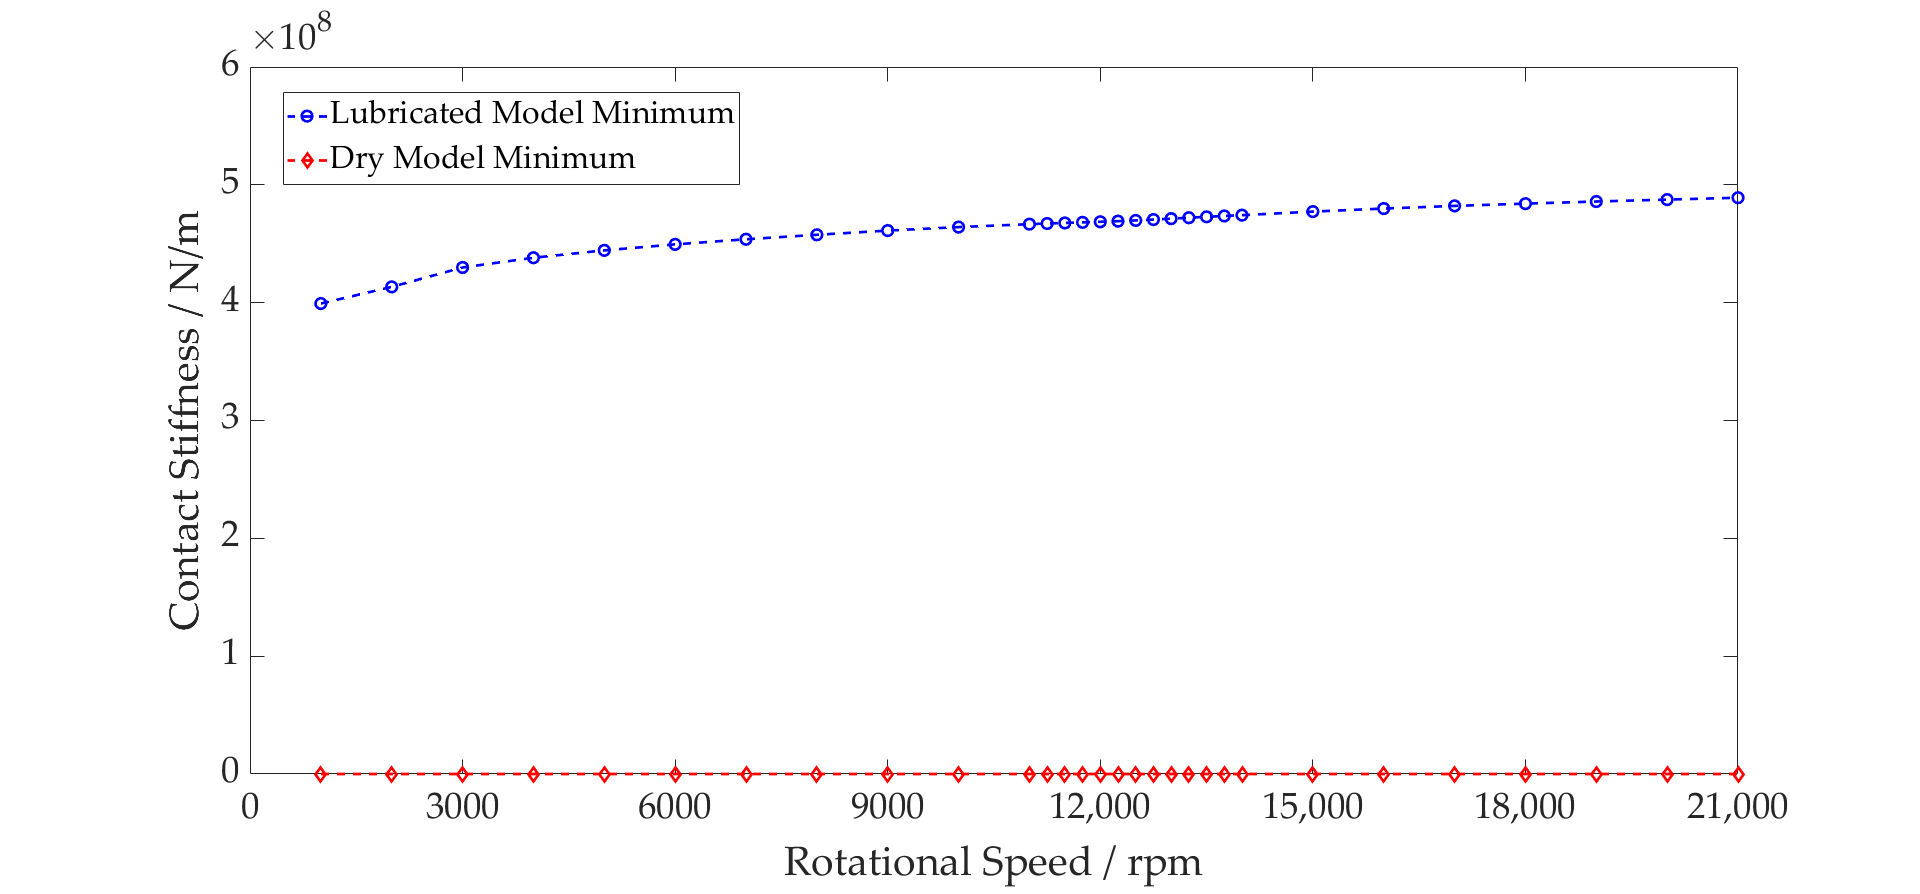
\includegraphics[width=150mm]{FlexiTribo Figure 12. Rolling Element Contact Stiffness - Dry vs Lubricated Minimum Values.png}
	\caption{Rolling element contact stiffness - Dry vs lubricated minimum values.}
	\label{Rolling element contact stiffness - Dry vs lubricated minimum values}
\end{figure}

Analysing the conjunction level results from the lubricated model, the contact force due to the gear mesh frequency is shown superimposed on the ball pass frequency as an individual element passes through the loaded region of the bearings (Figures \ref{Film thickness vs contact force 21 000 rpm} and \ref{Film thickness vs contact force 12 500 rpm}). The higher contact forces result in a reduction in the central film thickness, also shown when observing the variation in film thickness for both plots. At 12~500~$\mathrm{rpm}$, the force and film thickness fluctuations are much larger due to the high excitation levels of the shaft during resonance. At 21~000~$\mathrm{rpm}$, even with a much lower torque transfer through the gear pair, the contact forces are greater than at 12~500~$\mathrm{rpm}$. This is due to the contribution of the film enhancing the total contact deflection and hence increasing the contact force.

\begin{figure}  
	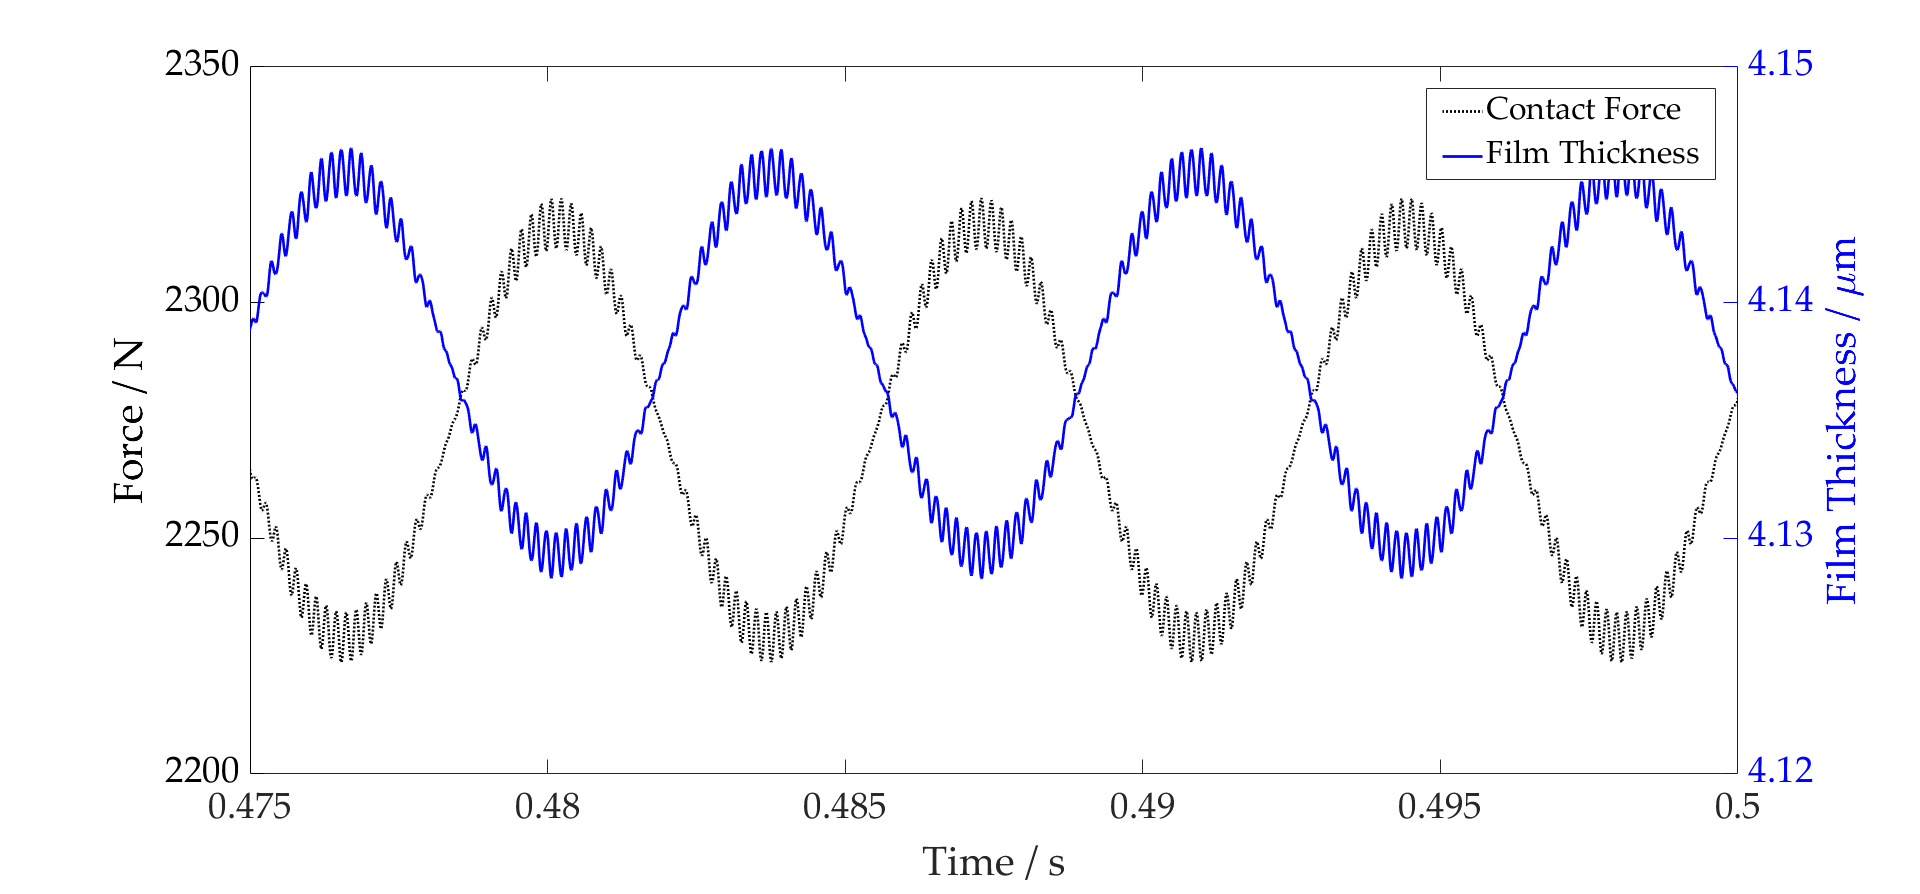
\includegraphics[width=150mm]{FlexiTribo Figure 13. Film Thickness vs Contact Force 21 000 rpm.png}
	\caption{Film thickness vs contact force 21~000~$\mathrm{rpm}$.}
	\label{Film thickness vs contact force 21 000 rpm}
\end{figure}

\begin{figure}  
	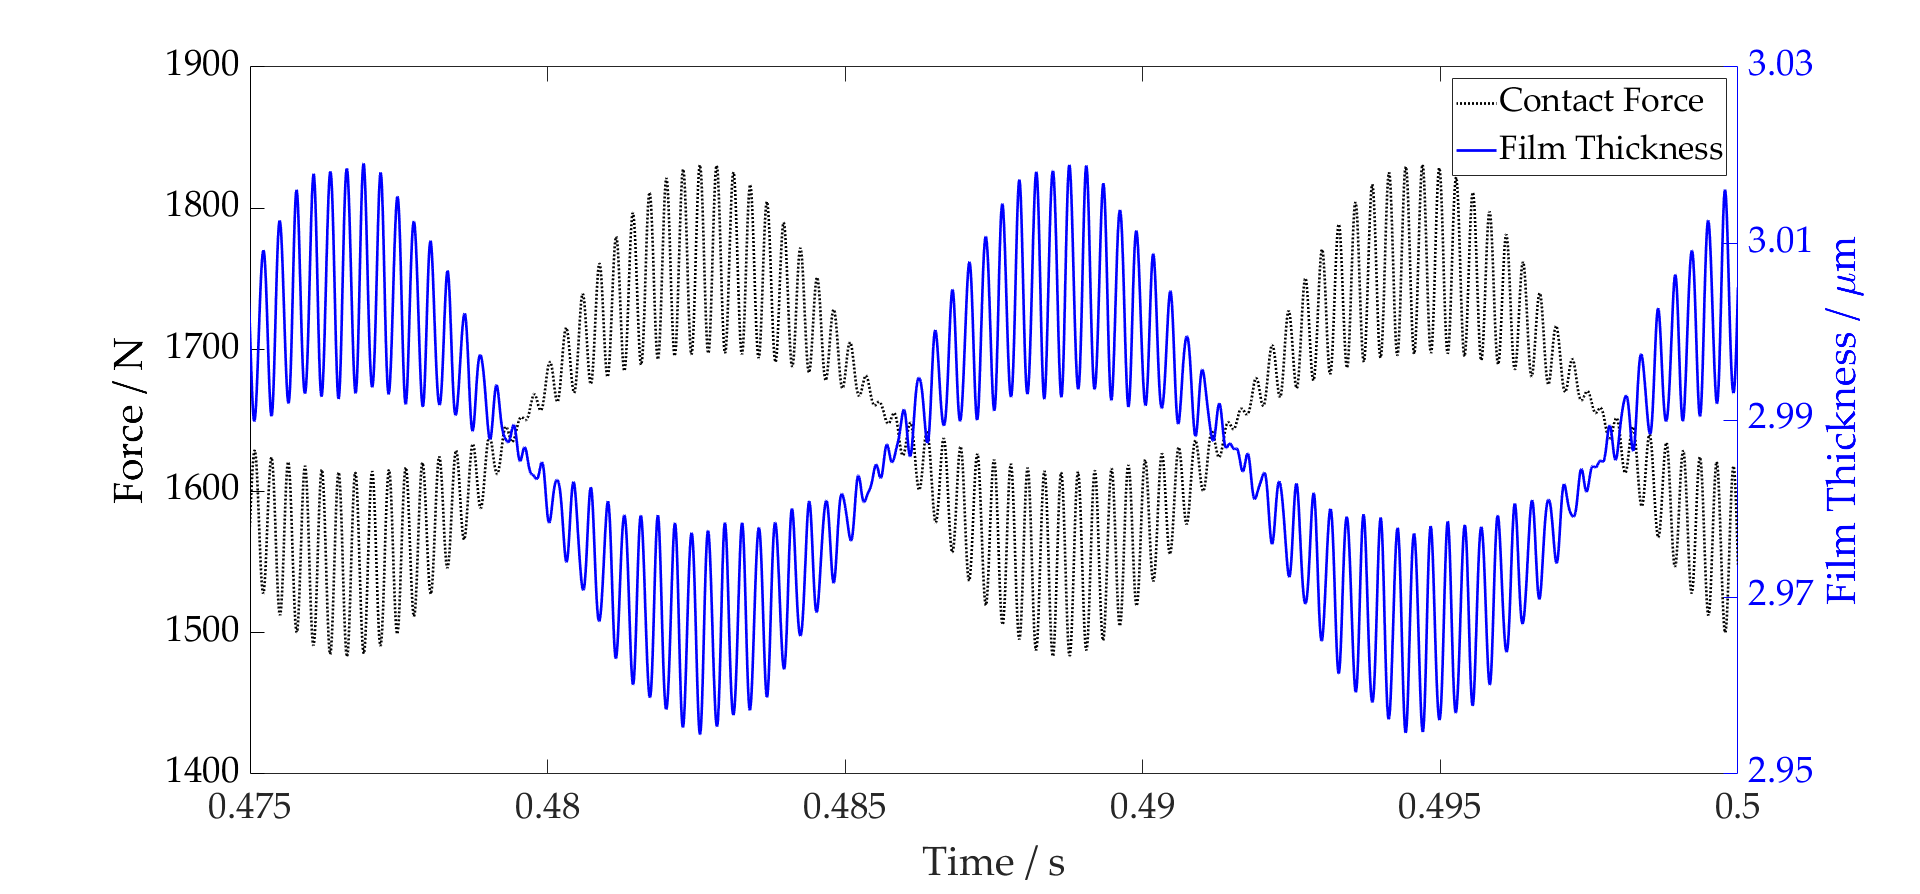
\includegraphics[width=150mm]{FlexiTribo Figure 14. Film Thickness vs Contact Force 12 500 rpm.png}
	\caption{Film thickness vs contact force 12~500~$\mathrm{rpm}$.}
	\label{Film thickness vs contact force 12 500 rpm}
\end{figure}

\subsection{Conclusions}

The new methodology presented has been developed to implement a lubricated bearing model within a flexible system level model. The model implicitly includes the lubricant film at the roller–race contact within the bearing; this is something that has not, to the authors’ knowledge, been reported previously in the open literature. Simulations have been performed up to 21~000~$\mathrm{rpm}$ with realistic excitation forces from a first stage reduction gear pair and electric motor. The conjunction level and system level results have been analysed to compare the lubricated and conventional dry-bearing modelling techniques in a flexible  multi-body dynamic (FMBD) environment.

Results show that the film thickness reaches 4.1521~${\mu m}$ at 21~000~$\mathrm{rpm}$. This leads to 9.6 times greater contact forces and hence 24.9\% greater contact stiffness between the dry and lubricated models due to the lubricant entrainment and non-linear Hertzian force–deflection relationship. The contribution of all the rolling elements leads to the lubricated model having a 16.6\% greater maximum total bearing stiffness at 21~000~$\mathrm{rpm}$ than the dry model. Moreover, this stiffness is shown to increase with speed due to the film thickness increasing with the entrainment velocity; this is something that dry models do not account for.

This increase in the total bearing stiffness leads to a change in the stiffness of the total system. By modelling the shaft as a flexible body, the influence on the natural frequency of the system is seen. The resonant peak at 12~500~$\mathrm{rpm}$ shifts 250~$\mathrm{rpm}$ higher in the lubricated model, which coincides with the higher frequency excitation from the gear meshing.

Understanding the influence of the roller bearings on the transmission stiffness is of particular importance in automotive applications, and this change shows the effect of the lubricant film on the already complex contact phenomena. Neglecting the effect of the lubricant film can lead to an underestimation of the bearing stiffness, impacting the accuracy of dynamic analyses such as noise, vibration and harshness (NVH) prediction. As transmissions operate at higher speeds with more complex interconnected structures and noise paths, it is important that these behaviours are modelled accurately. Furthermore, underestimation of the contact forces will also lead to a miscalculation of contact pressures, impacting future sub-surface stress and wear analyses for the life predictions of these crucial critical  machine elements.

Further developments of this work aim to include more complex rheological phenomena, accounting for thermal and starvation effects at high speeds. Computational efficiency must also be maintained when embedding these models within FMBD environments, due to the iterative nature of the EHL solution.

The presented work establishes the necessity of a multi-physics approach to model the tribology and dynamics of high-speed rolling element bearings. This is essential for future powertrain modelling to ensure accurate component and system level behaviour.




%\chapter{Artificial Neural Networks for EHL Film Thickness Predictions}
\label{ANN Lubricated Bearing FMBD}

\section{Introduction}

Tribodynamic modelling generally employs analytical equations for the prediction of film thickness in elastohydrodynamic contacts; chosen due to their timely solution. Whilst computationally efficient, these do not achieve the accuracy of the full numerical solution outside the bounds of the data used to generate the analytical equations. In the context of dynamic simulation, a full numerical solution at each time step of a system level model would, however, yield excessive computation time. This has led to the emerging use of data driven solutions, such as machine learning, in the field of tribology. These can achieve accuracy much closer to the numerical solution, whilst significantly improving computational time.

This chapter details the development of an ANN for prediction of central film thickness at the roller-race conjunction. ANNs are trained using data generated by numerical solution, with the data set constrained to realistic operating conditions using the Greenwood regimes of lubrication. Multiple ANNs are compared to find the optimum structure, accounting for training time and accuracy.

This workflow introduces the application of Artificial Neural Networks (ANNs) a form of Machine Learning (ML) algorithm, to predict the central film thickness at the roller-race conjunction. The performance of ANNs will be compared with analytical equations and numerical solutions, assessing the suitability of its implicit application within FMBD environments. The aim is to improve the accuracy of the central film thickness estimation, whilst maintaining a timely solution in the context of a full dynamic solution.

\section{Numerical vs Analytical Film Thickness Estimations at High Entrainment Velocities}

Two main approaches exist for determination of the complex non-linear problem of film thickness in lubricated contacts. The first approach involves employing numerical methods \cite{Dowson1959}, where systems of partial differential equations are formulated to describe the state of the contact and then solved iteratively \cite{Gohar2018}. While this method yields accurate results and is applicable to a wide range of operating conditions, it is computationally intensive due to its iterative nature. The second approach involves developing regressed analytical equations from experimental or numerical studies which can be used for specific lubrication regimes. These equations offer quick estimates of key parameters, such as central \cite{Dowson1979} and minimum film thickness \cite{Dowson1967}. However, whilst more computationally efficient than the full numerical solution, this approach has limitations. 
The applicability of regressed equations is often limited to the range of data used for their development, resulting in reduced accuracy due to simplification. There is also a requirement for extensive effort in collecting experimental or numerical data to develop them. 

Comparison graphs

Timing for each points

Error between both

Emphasis that this discrepancy must be overcome

The implementation of ANNs within tribology is one way to overcome the computational expense of the full numerical solution and the limited validity of the analytical approach.   To ensure the validity of the ANN, a methodology is suggested for training it within a range consistent with the numerical solver.

\section{Machine Learning Fundamentals}

Artificial intelligence (AI) refers to machines that exhibit human cognitive skills. They are a set of algorithms which allow machines to learn and problem solve in a manner inspired by the neurons in the human brain. Machine learning (ML), a subset of AI, allow systems to perform tasks without explicit programming. These algorithms analyse data and autonomously adapt to enhance their task performance, resembling the human ability to learn from experience. 

ML encompasses two primary algorithm types: supervised learning and unsupervised learning. In supervised learning, the program receives both input data and target outputs. The programmer guides the algorithm by demonstrating the correct output. The program can then compare its own outputs to the desired ones, refining itself through training. For example, by training on images and corresponding object names, the program can subsequently recognize objects in new images unassisted. Unsupervised learning algorithms operate without target outputs, exploring input data for patterns independently. These algorithms analyse the input's feature space and cluster the data accordingly. When presented with new data, the program assigns it to an existing cluster based on its location in the feature space.

ML algorithms can also be classified based on the type of output they produce. They can be utilized for classification problems, where data points are assigned to discrete categories, or regression problems, involving approximating continuous output functions. Classification tasks can be accomplished through supervised learning algorithms using logistic regression, approximating step functions with discrete outputs. Unsupervised learning algorithms achieve classification through clustering, an example of which being character recognition and speech processing,image and speech processing.

Supervised ML algorithms have the advantage of approximating continuous output functions, making them suitable for complex nonlinear relationships between inputs and outputs. By comparing their outputs with target values during training, they act as universal function approximators. This characteristic proves particularly valuable for applications such as tribological simulation, where the interaction between contacting surfaces requires efficient solvers. Notably, supervised linear regression ML algorithms offer effective solutions in this domain.

Literature review concluded this is best approach

An Artifical Neural Network (ANN) is a computational model which is inspired by the neural networks present in the human brain. It is a subset of machine learning.

ANNs are made up of a set of interconnected nodes that have the ability to adapt to input data for the purpose of solving complex non-linear functions. The nodes, known as artificial neurons, are organized into layers. The three main types of layers are shown in FIGURE 1, these are: Input layer; Hidden layer(s) and Output layer. The adaptation is performed using weighted connections, that connect each neuron layer. These weightings can be adapted during the learning process, and determine the strength of the connections between neurons.

The generalized structure of an ANN comprises several layers which contain neurons inside. Equation \ref{Generalized ANN} describes the relationship between each neuron, $i$, of each layer, $j$,

\begin{equation}\label{Generalized ANN}
	u_i^{j, k}=f_j\left(\sum_{\forall m} W_i^{j, k} \cdot x_m+b_i^{j, k}\right)
\end{equation}


\section{Methodology}

Overall workflow flowchart

\begin{figure}  
	\centering
	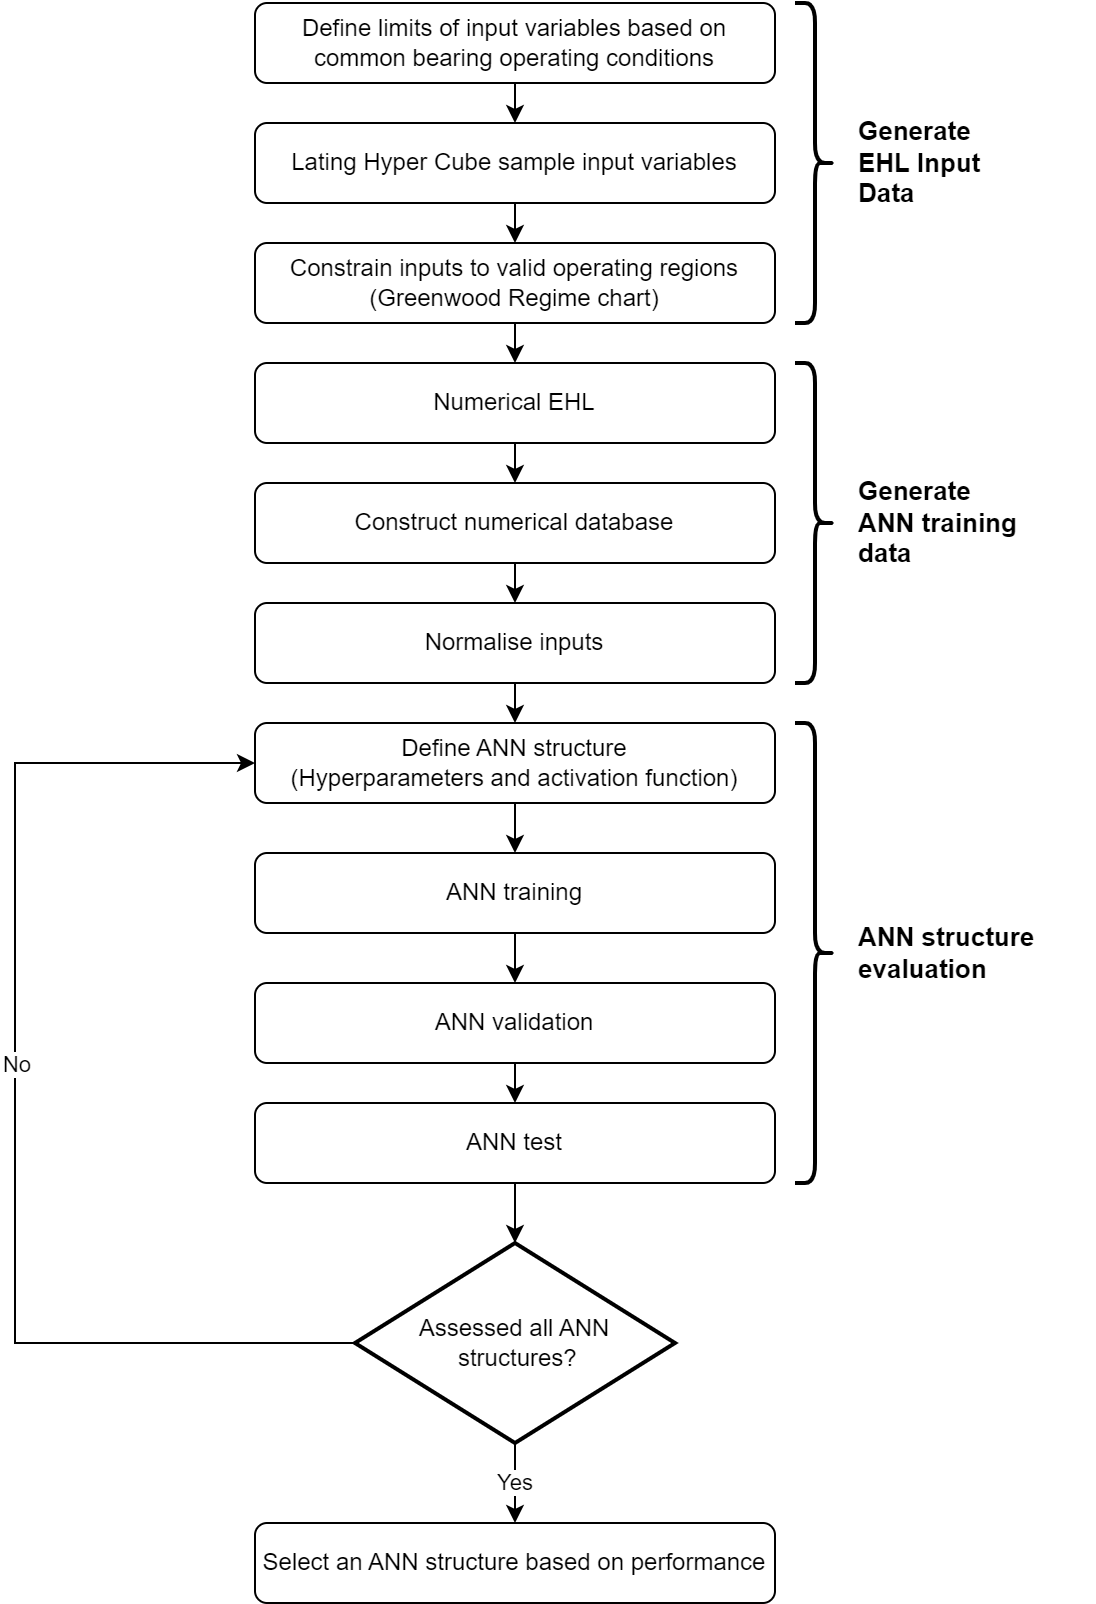
\includegraphics[width=105mm]{ANN_structure_flowchart.png}
	\caption{ANN data flow, models and training flowchart}
	\label{ANN flowchart}
\end{figure} 



\subsection{ANN Structure}


The learning process of an ANN involves training a set of input data which correspond to known output values. A common technique for this is backpropagation, where the connection weightings in the network are adjusted such that the error between the predicted and the actual output are minimized. The goal of this training is to minimize the error, and to improve the ability of the network to generalize and make accurate predictions for new, unseen data. By this method, complex, non-linear functions such as the EHL film thickness estimation can be performed.

As the structural complexity of ANNs increases, the training time increases due to the greater number of neurons and layers. Implementations of ANN in the field of tribology, specifically film thickness predictions, are typically limited to between one and three hidden layers \cite{Marian2021}.

The structure of the ANN is described in the following format, as per \cite{Zhang2002}:

\begin{equation}
	N_{i n}-\left[N_{h 1}-N_{h 2}-N_{h 3}\right]_t-N_{\text {out }}
\end{equation}

The number of neurons in each layer is denoted by $N$, with the input and output layers indicated by the subscripts $in$ and $out$, respectively. Subscripts $h1$, $h2$, and $h3$ denote the hidden layers, with $t$ being the total number of hidden layers. A graphic representation of the structure used for the film thickness estimations is show in Figure \ref{ANN structure}.

\begin{figure}  
	\includegraphics[width=150mm]{ANN_Structure.png}
	\caption{ANN structure to predict EHL central film thickness ($9-[14-14-14]_3-1$)}
	\label{ANN structure}
\end{figure} 

The structure of an ANN affects both its training time and prediction accuracy. To evaluate the performance of different ANN structures, and hence select an appropriate structure for this application, a sensitivity study was performed. In this study, the input data range remained constant across all structures, while the variables listed in Table \ref{Sensitivity study of ANN structure} were adjusted:

Selection of the final structure for suitability analysis was based on total training time, coefficient of determination ($R^2$), and the potential for the ANN to overfit. Overfitting is the phenomenon whereby an ANN becomes too specialised at learning the training data, and as a result performs poorly with new, unseen data. This occurs when the network extensively adjusts its internal parameters to fit noise or outliers in the training set \cite{Ying2019}.

\begin{table*}
	%\captionsetup{justification=centering}
	\caption{Sensitivity study of ANN structure}
	\label{Sensitivity study of ANN structure}
	\centering
	\renewcommand{\arraystretch}{1.5}%
	\begin{tabular}{|P{0.4\textwidth}|P{0.4\textwidth}|}
		\hline
		\textbf{Variable} & \textbf{Value} \\ [0.5ex]
		\hline
		Number of training data points & 600 - 1500 \\ [0.5ex]
		\hline
		Number of hidden layers, t & 1 - 4 \\ [0.5ex]
		\hline
		Number of neurons, N & 10 - 20 \\ [0.5ex]
	    \hline
		Activation function type & Hyperbolic tangent, Logistic sigmoid, Rectilinear \\ [0.5ex]
		\hline
	\end{tabular}
\end{table*}

\paragraph{Data Normalization}

Normalization of the input and target parameters is first performed using min-max normalisation function:

\begin{equation}
	\tilde{x}=\frac{x-x_{\min }}{x_{\max }-x_{\min }}(u-l)+u
\end{equation}

where $u$, and $l$ represent the upper and lower normalized unit values of 1 , and -1 respectively. The dimensional target input value is denoted by $x$, and the final normalised input or output parameter of the ANN is denoted by $\tilde{x}$. In order to dimensionalise the output layer, $x_{\max }, x_{\min }$ must be stored as a variable.

\paragraph{Training, Validation and Test Datasets}

The dataset is divided into three sets: the training set, the validation set, and the test set, each containing 70~$\%$, 15~$\%$ and 15~$\%$ of the training data respectively:

\begin{enumerate}
	\item Training Set: The training set is the portion of the dataset used to train the ANN, containing the input data and the corresponding output data. As aforementioned, the ANN adjusts the internal parameters based on this data to learn the underlying patterns.
	\item Validation Set: The validation set is used to tune the performance of the ANN during the training process. It is an independent dataset that the network has not seen before, allowing for the evaluation of its generalization capabilities. The network's performance on the validation set is monitored during training to make decisions on adjusting hyperparameters (number of hidden layers, neurons per hidden layer, activation functions etc.) or stopping the training process to prevent overfitting.
	\item Test Set: The test set is a completely independent dataset that is not used during training or validation. It is used to assess the final performance and generalization ability of the trained ANN. By evaluating the network on unseen data, the test set provides an unbiased estimate of the model's performance in actual use.
\end{enumerate}

For this sensitivity study, the size of the training data set was varied (600, 1000, 2000 and 5000) to observe the its effect on the quality of the prediction. A limit of 1000 epochs was also implemented. This limits the ANN to 1000 full iterations through the entire training set during training. This was found to be sufficient to improve accuracy whilst preventing overfitting of the data.

\paragraph{Evaluating the Network Performance}

During backpropagation of the ANN, the Mean Squared Error (MSE) was used to evaluate the network's performance:

\begin{equation}\label{MSE}
	M S E=\frac{1}{N} \sum_{i=1}^N\left(t_i-y_i\right)^2
\end{equation}

where $t_i$ and $y_i$ are the target and predicted value respectively. The total number of training points being trained, validated or tested is denoted by $N$. 

To assess the goodness of fit of the ANN, the statistical metric $R^2$ known as the coefficient of determination was used. This measures the proportion of variance in the dependant variable (output film thickness) that is predictable from the input variables (Table \ref{Range of ANN film thickness calculation parameters}) in the model. This value ranges from 0 to 1, with a higher value indicating the best fit of the model to the data. This was post-processed after training and is calculated as follows:

\begin{equation}\label{R-squared}
	R^2=1-\frac{\sum_{i=1}^N\left(t_i-y_i\right)^2}{\sum_{i=1}^N\left(y_i-\bar{y}\right)^2}
\end{equation}

 where $\overline{\mathrm{y}}$ is the mean of the target sample. The numerator of the fraction, \( \sum_{i=1}^N(t_i - y_i)^2 \), represents the sum of squared residuals, which quantifies the variation in the target variable that is not explained by the model. The denominator, \( \sum_{i=1}^N(y_i - \bar{y})^2 \), is the total sum of squares, which captures the total variation in the target variable \cite{Marian2022}.

\paragraph{Activation Functions}

Activation functions are mathematical functions that are applied to the output of each neuron in a layer of the neural network. These introduce non-linearity which allow the network to learn complex input-output relationships. Activation functions help determine the  output of a neuron based on the weighted sum of its inputs.

As suggested in \cite{Marian2022}, suitable activation functions for the hidden layers are as follows:

\begin{itemize}
	\item Sigmoid (logistic): This function transforms the input values into a range between 0 and 1. It has continuously differentiable smooth S-shaped curve and is given by the following formula \cite{Han1995}:
	
	\begin{equation}\label{Logistic sigmoid}
		\log \operatorname{sig}(x)=\frac{1}{1+e^{-x}}
	\end{equation} 
	
	Sigmoid functions are commonly used in the hidden layers of ANNs, however may suffer from the "vanishing gradient" problem where the partial derivative reaches zero \cite{Sharma2020}, leading to slower convergence during training.
	
	\item ReLU (Rectified Linear Unit): This function is the most commonly used activation function. It outputs the input value directly if it is positive, and zero otherwise. The mathematical definition is:
	
	\begin{equation}\label{ReLU}
		\operatorname{ReLU}= \begin{cases}x, & x \geq 0 \\ 0, & x \leq 0\end{cases}
	\end{equation}
	
	The gradient is 1 when the neuron is activated, and zero when it is deactivated. This function is computationally efficient and addresses the vanishing gradient problem to an extent \cite{Sharma2020}.
	
	\item Tanh (Hyperbolic Tangent): The hyperbolic tangent or tanh function is defined as:
	
	\begin{equation}\label{Hyperbolic tangent}
		\tanh (x)=\frac{2}{1+e^{-2 x}}-1
	\end{equation}
	
	The formulation and behaviour is very similar to sigmoid. It produces values which range from -1 to 1, having a centred mean around zero. Like sigmoid, this also experiences vanishing gradients.
	
	\item Linear: A simple linear activation was used on the output.
	
\end{itemize}

Early stopping and regularisation was used to prevent statistical overfitting during training \cite{MatlabOverfit}. Early stopping halts the training process before the model reaches the maximum number of epochs. This is done by monitoring the performance (MSE (Equation \ref{MSE})) of the network against the validation set during training. Once the performance reaches a plateau, or begins to degrade, the training is stopped early. Regularisation adds additional constraints to the learning process. It modifies the performance criteria by accounting for the change in mean square of the network weights and biases (Mean Squared Weight (MSW)). This is calculated in Eq. \ref{MSW}: 

\begin{equation}\label{MSW}
	M S W=\frac{1}{N} \sum_{j=1}^N w_j^2
\end{equation}

where $w_j$ is the individual weight value associated with the $j$-th neuron or connection in the network.

By applying an adjustment factor, denoted as $\gamma^{\prime}$, the weights and biases can be reduced during propagation (Eq. \ref{MSE adjusted}), thus mitigating the risk of overfitting and improving the network's generalization capability.

\begin{equation}\label{MSE adjusted}
	M S E_{r e g}=\gamma^{\prime} * M S W+\left(1-\gamma^{\prime}\right) * M S E
\end{equation}


\subsection{ANN Input Data Generation}

Training an ANN requires an often comprehensive data set. For the purpose of this study, the training data was generated using the numerical EHL model presented in \ref{1D EHL Model}. This decision was made due to the size of the database required for training, and the timely and relatively low resource-intensive nature to generate this. It is worth noting that training data could also be obtained from experimental work, which further enhances the applicability of this approach for future studies.

\subsubsection{Numeric Database Construction}

Due to the large design space covered by the high number and range of input parameters, a robust sampling technique needs to chosen to create the training data set. In traditional random sampling, each of the parameters is randomly sampled within its defined range. This may lead to insufficient coverage of the parameter space and simple bias, as this method has no "memory" of points already selected.

The Latin Hypercube Sampling (LHS) method was utilised by Marian et al. \cite{Marian2022}, and was chosen for this study. LHS is a statistical method commonly used in experimental design and statistical analysis to efficiently sample a high-dimensional parameter space. It generates a near-random sample of parameter values from multi-dimensional distributions. The sample points are distributed such that the design space is filled as evenly as possible, with information from nearly all regions being covered. This ensures lower computational effort required for ANN training, despite the high number of input variables and value ranges. 

LHS is based on the concept of Latin hypercube design (LHD). In LHD, the parameter space is divided into equal intervals along each dimension. Each interval is then randomly assigned to a unique position within its corresponding dimension. The process results in a matrix, where each row represents a combination of parameter values. Contrary to the random sampling method, LHD guarantees that only one sample is taken from each row, ensuring a diverse and representative set of samples.

The LHD is a $n_{\mathrm{s}} \times n_{\mathrm{f}}$ matrix, where $n_s$ and $n_f$ represent the number of simulations the number of factors respectively. LHS enhances LHD by introducing a randomization component. The randomly selected samples within each interval are shuffled, ensuring that samples are not biased by the order of selection.

LHS elements are generated by subtracting a random number between zero and one $Z_{\mathrm{r}}[0,1)$ from each LHD element $x_{i j, \mathrm{LHD}}$. This is then divided by the number of test points \cite{Siebertz2010}:

\begin{equation}\label{LHS}
	x_{i j, \mathrm{LHS}}=\frac{x_{i j, \mathrm{LHD}}-Z_{\mathrm{r}}[0,1)}{n_{\mathrm{s}}}
\end{equation}

This equation rescales the LHD values to a range between 0 and 1. By subtracting a random number between 0 and 1 and dividing by the total number of sample points, the resulting Latin hypercube samples are spread evenly across the interval (0,1) for each parameter. This is important, because it allows the Latin hypercube samples to be easily transformed to any desired range or distribution.

The quality of the test field (freedom of correlation and uniform distribution) can be assessed based on the distances between data points \cite{Johnson1990}. The MaxiMin criterion in MATLAB's Statistics and Machine Learning toolbox was used to optimise the LHS. This maximises the the minimum distance between individual test points such that the LHS test field is uniformly distributed:

\begin{equation}\label{maximin}
	\operatorname{MaxiMin}=\left[\sum_{1 \leq i<j \leq n_1} d\left(x_i, x_j\right)^{-\xi}\right]^{-\frac{1}{\xi}}
\end{equation}

where $d$ represents all distances in the test field, and subscripts $i$ and $j$ are indexes for the parameter and sample point respectively. $\xi$ represents the application dependant factor which determines the degree of importance assigned to the distances \cite{Siebertz2010}.



Marian et. al conducted a study for film thickness distribution
%explain the study
%explain the methods
%explain the outcome and why I decided to us ANN
%also explain Ani study


SECTION ON LHS AND PARAMETER STUDY COMPARISON (ANI)



\subsubsection{Constraining the Input Data Bounds}

The performance of ANNs is heavily reliant upon the quality of the data set provided for training. To construct a training database, Marian et al. \cite{Marian2022} utilised a Finite Element Method (FEM) solver. The database covered a very large range of lubricant and material properties for relatively low entrainment speed conditions (< 0.4~$m/s$ for the 2D line contact studies). The resulting contact conditions when some combinations of these parameters were used, exceeded realistic conditions within common machine elements, including bearings. Since the film thickness evaluation is required for the EHL contact of roller bearings, the input data set for this study requires constraining to improve validity.

A method to constrain the input parameter combination to realistic machine element operating points was devised. The Greenwood Regime chart \cite{Johnson1970} was used for this purpose. The regions of the chart, as shown in Fig.XXXX, are:

\begin{itemize}
	\item Isoviscous Rigid (IR)
	\item Isoviscous Elastic (IE)
	\item Piezoviscous Rigid (PR)
	\item Piezoviscous Elastic (PE)
\end{itemize}

The bounds indicate the transition between the lubrication regimes, which are classified based on material, rheological and geometric properties. To find which regime a contact is operating within, the dimensionless elasticity ($G_e$) and viscosity ($G_v$) parameters can be calculated:

\begin{equation}\label{G_e}
	G_e=\left(\frac{\alpha^2 W_i^3}{\eta_0 u R_r^2}\right)^{\frac{1}{2}}
\end{equation}

\begin{equation}\label{G_v}
	G_v=\left(\frac{W_i^2}{\eta_0 u E_r R_r}\right)^{\frac{1}{2}}
\end{equation}

The PE region signifies contact pressures high enough to elastically deform the material and increase the viscosity of the lubricant; hence an EHL contact. The IR region relates to the hydrodynamic regime of lubrication, where the contact is lightly loaded and the surfaces do not deform and viscosity does not increase. Since these investigations are focussed on improving the EHL film thickness solution, the training data set was required to fall within the PE region of the Greenwood plot. The initial range of each parameter is shown in Table \ref{Range of ANN film thickness calculation parameters}. The training data set was then generated using these limits. The input data was then constrained further to ensure Hertzian pressures fell between 300~$MPa$ and below 3.5~$GPa$, as well as redistributing any points that fell outside of the PE and PR regions. HOW IS THIS DONE. SHOW BEFORE AND AFTER PLOTS AND INFLUENCE ON TRAINING QUALITY?

\begin{figure}  
	\includegraphics[width=150mm]{ANN_Explicit_MarianvsGreenwood.png}
	\caption[Greenwood informed training data vs Marian et al.]{Greenwood informed training data vs Marian et al. \cite{Marian2022}.}
	\label{Greenwood informed training data vs Marian et al.}
\end{figure} 

\begin{table*}
	%\captionsetup{justification=centering}
	\caption{Range of ANN film thickness calculation parameters}
	\label{Range of ANN film thickness calculation parameters}
	\centering
	\renewcommand{\arraystretch}{1.5}%
	\begin{tabular}{|P{0.4\textwidth}|P{0.15\textwidth}|P{0.15\textwidth}|P{0.15\textwidth}|}
		\hline
		\textbf{Parameter} & \textbf{Unit} & \textbf{Minimum} & \textbf{Maximum} \\ [0.5ex]
		\hline
		Load & $N$ & 150 & 5000 \\ [0.5ex]
		\hline
		Entraining Velocity & $m/s$ & 0.6 & 30 \\ [0.5ex]
		\hline
		Reduced Radius & $m$ & 0.0001 & 0.02 \\ [0.5ex]
		\hline
		Reduced Elastic Modulus & $GPa$ & 200 & 250 \\ [0.5ex]
		\hline
		Pressure-Viscosity Coefficient & ${GPa}^{-1}$ & 10 & 30 \\ [0.5ex]
		\hline
		Reference Viscosity & $Pa.s$ & 0.0005 & 0.1 \\ [0.5ex]
		\hline
		Maximum Density & ${kg}/{m}^3$ & 7750 & 8050 \\ [0.5ex]
		\hline
		Poisson's Ratio & $-$ & 0.3 & 0.35 \\ [0.5ex]
		\hline
		Contact Length & $m$ & 0.001 & 0.050 \\ [0.5ex]
		\hline
		
	\end{tabular}
\end{table*}

\textbf{CHECK THIS}The numerical solution database can also benefit from explicit parallelisation ie. use of multiple computational cores of the CPU. When using MBD solvers implicitly it is not possible to use explicit parallelisation since a particular time step is dependent on the present timestep as well as on data of the same timestep. The ANN functionality in turn can be embedded with an implicit MBD computation environment to significantly improve the computation times without the need of explicit parallelisation despite benefitting from it indirectly. 








\subsection{Explicit Bearing Film Thickness Predictions}

The same FMBD model used in Chapter \ref{Lubricated FMBD} was used for this study. The shaft was modelled as a rigid body, and loading was purely static in one radial direction to remove the influence of dynamic effects. The shaft is constrained to one rotational and two lateral degrees of freedom. Bearing properties and operating conditions are shown in Table \ref{Roller bearing parameters} and Table \ref{Operating Conditions} respectively.

\begin{table*}
	%\captionsetup{justification=centering}
	\caption{Roller Bearing Parameters}
	\label{Roller bearing parameters}
	\centering
	\renewcommand{\arraystretch}{1.5}%
	\begin{tabular}{|c|c|}
		\hline
		\ \textbf{Parameter} & \textbf{Value} \\ [0.5ex]
		\hline
		Inner race diameter & 31.5 $mm$ \\ [0.5ex]
		\hline
		Roller diameter & 7.5 $mm$ \\ [0.5ex]
		\hline
		Roller length & 15 $mm$ \\ [0.5ex]
		\hline
		Number of rollers & 12 \\ [0.5ex]
		\hline
		Radial interference & 5 $\mu \mathrm{m}$ \\ [0.5ex]
		\hline
		Young's modulus & 218 $GPa$ \\ [0.5ex]
		\hline
		Poisson's ratio & 5 $0.3$ \\ [0.5ex]
		\hline
	\end{tabular}
\end{table*}

\begin{table*}
	%\captionsetup{justification=centering}
	\caption{Operating Conditions}
	\label{Operating Conditions}
	\centering
	\renewcommand{\arraystretch}{1.5}%
	\begin{tabular}{|c|c|}
		\hline
		\ \textbf{Parameter} & \textbf{Value} \\ [0.5ex]
		\hline
		Radial force & 2500 $N$ \\ [0.5ex]
		\hline
		Rotational velocity & 10~000$rpm$ \\ [0.5ex]
		\hline
	\end{tabular}
\end{table*}

The dynamic model was run explictly as a dry model, without the influence of the EHL film at the roller-race contacts. The kinematic and dynamic results required for input to the ANN are then extracted at each time step. Results were generated for an individual element completing one complete orbit around the bearing. Extracted results include roller load per unit length, reduced radius of the contact between the roller and inner-race, and the contact entrainment velocity.

The loading pattern is cyclic in nature as the roller enters and exits the most highly loaded region of the bearing, corresponding to the force vector applied to the inner race. Sufficient preload ensures constant contact between elements and raceways so that the regime does not deviate from EHL. The contact reduced radius and entrainment speed do not change throughout the orbit as they are a function of bearing geometry and constant operating speed.

\begin{figure}
	\centering
	\begin{subfigure}[b]{0.9\textwidth}
		\centering
		\includegraphics[width=\textwidth]{ANN_Explicit_Bearing Normal Load.png}
		\caption{}
		\label{Contact Normal Load ANN}
	\end{subfigure}
	\hfill
	\begin{subfigure}[b]{0.9\textwidth}
		\centering
		\includegraphics[width=\textwidth]{ANN_Explicit_Bearing Entrainment Velocity.png}
		\caption{}
		\label{Contact Entrainment ANN}
	\end{subfigure}
	\hfill
	\begin{subfigure}[b]{0.9\textwidth}
		\centering
		\includegraphics[width=\textwidth]{ANN_Explicit_Bearing Reduced Radius.png}
		\caption{}
		\label{Contact Reduced Radius ANN}
	\end{subfigure}
	\caption{Individual rolling element input values to ANN : a) Contact load, b) Contact entrainment velocity, c) Contact reduced radius}
	\label{Individual rolling element input values to ANN}
\end{figure}


\subsection{Implicit Bearing Film Thickness Predictions}



\section{Results and Discussion}

The following data was obtained using consumer grade hardware with the following specifications: 
Intel® Core™ i7-9750H CPU 6 cores @ 2.60GHz, 32GB RAM; GPU: NVDIA GeForce GTX 1650.

The same hardware was used for both the full numerical and the ANN solutions to provide performance comparisons and assess the suitability of ANNs for film thickness calculations in FMBD solvers.

\subsection{ANN Structure and Performance}

The 1D EHL model presented in Section \ref{1D EHL Model} was used to generate the numerical database for training the ANN. Each numerical solution and hence training point took an average of 5.88~$s$. The construction of the entire database on a single core therefore has a wall time of between 58.8~$min$ and 489~$min$ for 600 and 5000 points respectively. This wall time is purely for baseline comparisons, and can be significantly improved using parallelisation across multiple cores.

A parameter study was conducted to determine the optimal structure for the ANN. Over 500 different structures were tested using the same input data. This involved varying the hyperparameters: the number of hidden layers varied from one to four, and the number of neurons from ten to twenty. The three aforementioned activation functions were explored in different hidden layer configurations. This included a combination of hyperbolic tangent in the hidden layers, with the final layer utilizing a logistic tangent function. For each configuration, the values of $R^2$ (coefficient of determination) and the training completion time were carefully documented.

Tables \ref{LogSig_table}-\ref{ANN_Explicit_LogSig_5000_table} present the $R^2$ values obtained from 600 data points, considering different activation functions, number of layers, and neurons. Among the activation functions tested, the ReLU function consistently underperformed when compared to the logistic sigmoid and hyperbolic tangent functions across all network structures. It is important to acknowledge that there is a slight variability in the performance of the network with each new training session. However, it is worth noting that the optimum number of layers, similar to tribological applications of ANNs \cite{Marian2021}, was found to be between two and three.

\begin{table}
	\caption{$R^2$ performance of ANN structures using 600 data points and a LogSig activation function}
	\label{LogSig_table}
	\includegraphics[width=\linewidth]{ANN_Explicit_ActFun_LogSig.jpg}
\end{table}

\begin{table}
	\caption{$R^2$ performance of ANN structures using 600 data points and a Tanh activation function}
	\label{Tanh_table}
	\includegraphics[width=\linewidth]{ANN_Explicit_ActFun_Tanh.jpg}
\end{table}

\begin{table}
	\caption{$R^2$ performance of ANN structures using 600 data points and a Tanh activation function}
	\label{ReLU_table}
	\includegraphics[width=\linewidth]{ANN_Explicit_ActFun_ReLU.jpg}
\end{table}

\begin{table}
	\caption{Training time of ANN structures with LogSig activation function and 600 data points}
	\label{ANN_Explicit_LogSig_600_table}
	\includegraphics[width=\linewidth]{ANN_Explicit_LogSig_600.jpg}
\end{table}

\begin{table}
	\caption{Training time of ANN structures with LogSig activation function and 1000 data points}
	\label{ANN_Explicit_LogSig_1000_table}
	\includegraphics[width=\linewidth]{ANN_Explicit_LogSig_1000.jpg}
\end{table}

\begin{table}
	\caption{Training time of ANN structures with LogSig activation function and 2000 data points}
	\label{ANN_Explicit_LogSig_2000_table}
	\includegraphics[width=\linewidth]{ANN_Explicit_LogSig_2000.jpg}
\end{table}

\begin{table}
	\caption{Training time of ANN structures with LogSig activation function and 5000 data points}
	\label{ANN_Explicit_LogSig_5000_table}
	\includegraphics[width=\linewidth]{ANN_Explicit_LogSig_5000.jpg}
\end{table}

\begin{figure}
	\centering
	\begin{subfigure}[b]{0.49\textwidth}
		\centering
		\includegraphics[width=\textwidth]{ANN_Explicit_600_Rval.png}
		\caption{}
		\label{600_Rval}
	\end{subfigure}
	\hfill
	\begin{subfigure}[b]{0.49\textwidth}
		\centering
		\includegraphics[width=\textwidth]{ANN_Explicit_1000_Rval.png}
		\caption{}
		\label{1000_Rval}
	\end{subfigure}
	\hfill
	\begin{subfigure}[b]{0.49\textwidth}
		\centering
		\includegraphics[width=\textwidth]{ANN_Explicit_2000_Rval.png}
		\caption{}
		\label{2000_Rval}
	\end{subfigure}
	\hfill
	\begin{subfigure}[b]{0.49\textwidth}
		\centering
		\includegraphics[width=\textwidth]{ANN_Explicit_5000_Rval.png}
		\caption{}
		\label{5000_Rval}
	\end{subfigure}
	\caption{$10-[14-14-14]_3-1$ using Hyperbolic Tangent activation function : a) 600 points, b) 1000 points, c) 2000 points, d) 5000 points}
	\label{$R^2$ performance of ANN structure}
\end{figure}







\subsection{Explicit Bearing Film Thickness Predictions}

After identifying suitable data set size and ANN structure, the ANN could then be compared to the analytical (Eq. \ref{DowsonToyodaCentralFilm}) and numerical (Section \ref{1D EHL Model}) methods of obtaining central film thickness at the roller-race contact. The operating conditions of the bearing were within the range of validity of the training data set. This is demonstrated in Figure \ref whereby the Greenwood parameters for the bearing operating points are overlayed on the training cloud.



\begin{figure}
	\includegraphics[width=150mm]{ANN_Explicit Film Thickness Comparisons.png}
	\caption{ANN, numerical and analytical central film thickness comparisons.}
	\label{ANN Film Thickness Comparisons}
\end{figure}
Figure 

Three different methods of obtaining the EHL film thickness were tested

\begin{tabular}{|c|c|c|}
	\hline \multirow{2}{*}{ Method } & \multicolumn{2}{|c|}{ Bearing } \\
	\cline { 2 - 3 } & Time per point & MSE \\
	\cline { 2 - 3 } & {$[\mathrm{s}]$} & {$[\mu \mathrm{m}]$} \\
	\hline Numerical & $4.87 \mathrm{E}+00$ & - \\
	\hline Analytical & $4.43 \mathrm{E}-05$ & $1.32 \mathrm{E}-3$ \\
	\hline ANN & $3.33 \mathrm{E}-03$ & $1.46 \mathrm{E}-8$ \\
	\hline
\end{tabular}

\subsubsection{Timing}
\subsubsection{Error}

\subsection{Implicit Bearing Film Thickness Predictions}

\subsubsection{Timing}
Each computational point, including 

\subsubsection{Error}


\section{Conclusions}
Roller bearings are only one application of these ANNs. The use cases extend far beyond roller bearings, to key components in automotive, machining and other industrial applications where interactions between contiguous surfaces exist. Film thickness is a critical parameter in the determination of NVH, friction and wear.

Full numerical solution can account for film thickness profile and pressure distribution across the contact. Futhermore, 

Echávarri et al. \cite{EchavarriOtero2014} comment on the "black box" nature of ANNs. Results from intermediate calculations are lost, which is often of interest for more in-depth analysis of contact condition; film thickness and pressure distributions and temperature for example.  


\chapter{Conclusions and Future Works}
\label{Conclusions}

\section{Overall Conclusions}

This thesis presents a coupled tribological and dynamic modelling approach to investigate the influence of the EHL film on bearing dynamics under electrified vehicle operating conditions. The following conclusions have been drawn from the results and analyses contained in this research:

\begin{enumerate}
	\item This work highlights the significant impact of the lubricant film on bearing dynamics, particularly at high-speeds where the EHL film thickness increases substantially. The film thickness can exceed that of the contact deformation predicted by the dry Hertzian assumption, significantly influencing contact force and stiffness predictions which are underestimated in non-lubricated analyses.
	\item A coupled simulation approach has been developed, integrating an implicit lubricated bearing model within system-level, FMBD model. Simulations were performed with representative electrified powertrain conditions. Results show that the lubricant film increases contact stiffness by up to 24.9~\% at 21~000~rpm when compared to conventional dry analyses. This results in a 16.9~\% increase in total bearing stiffness, shifting the system’s natural frequency and affecting the predicted NVH response. This emphasises the requirement to include the EHL film in dynamic analysis of electrified powertrains.
	\item At high entrainment velocities, it is shown that the analytical film thickness equations deviate from the numerical solution and underestimate the estimated film thickness.
	\item An ANN has been trained to predict EHL film thickness based on numerical data, with the training input data constrained using the Greenwood regimes of lubrication for enhanced accuracy. This overcomes the inaccuracies of the regressed equations at high entrainment velocities, and predicts film thickness with marginal error.
	\item The ANN approach demonstrated exceptional computational efficiency, achieving approximately 1~500 times faster central film thickness calculations than traditional numerical methods.
	\item The ANN has been embedded within an FMBD system model to calculate EHL film thickness and consider it implicitly in the evaluation of the bearing dynamics. This establishes a workflow that will further enhance contact modelling in FMBD simulations.
\end{enumerate}


\section{Contributions to Knowledge} \label{Contribution to Knowledge}

The main novelties and contributions to knowledge from this thesis are summarised below:

\begin{enumerate}
	\item A novel methodology to measure bearing orbital motion for tribological analysis at high-speed has been presented. This enabled component and conjunction level tribodynamic analysis of a roller bearing under previously unreported speeds and loading conditions.
	\item A coupled co-simulation approach was established to integrate an implicit lubricated bearing model within a high-speed system-level FMBD model. The lubricated bearing model considers the EHL film in the evaluation of the bearing and system dynamics. This was the first time a multi-physics model of this nature has been reported in open literature.
	\item An ANN was trained using input data from the numerical EHL solution. This was used to predict bearing film thickness across a wide range of tribological input variables. The methodology of constraining the training data using the Greenwood regime has not been openly reported, and ensured high data quality and hence accurate predictions. This methodology will further contribute to the accuracy of tribological ANNs.
	\item The ANN was embedded within an FMBD system model to calculate EHL film thickness and consider it implicitly in the evaluation of the bearing and system dynamics. The film thickness evaluation achieves the accuracy of numerical models without the associated computational limitations. This modelling method of combining component level ANN within a flexible system has not been previously reported.
\end{enumerate}

\section{Addressing the Research Questions}
The primary objective of this work was to investigate the interaction between tribology and dynamics in rolling element bearings, with particular focus on the significance of this multi-physics interaction in high-speed automotive applications. On reviewing the conclusions drawn from this thesis, it can be demonstrated that the research questions presented in Section \ref{Research Questions} have been addressed.

The findings of this thesis are to be implemented into the commercial software AVL EXCITE\textsuperscript{TM} M to support future rolling element bearing development. The influence of the lubricant film in dynamic analysis is of particular interest. The workflow of coupling contact level artificial neural networks into system level FMBD models is also of significance. This approach has applications beyond rolling element bearings, as a generic contact approach could also improve non-conformal contact modelling for gears and cams.

\section{Future Works}

The novel approaches presented in this thesis open up further opportunities to advance this area of research.

\begin{itemize}
	\item For wider adoption of the ANN solution, the ability to extrapolate beyond the bounds of the training data must be addressed. Extrapolation errors in film thickness estimation could affect the stability of an FMBD model and lead to divergence.
	\item Develop methodology for integrating ANNs into FMBD software. A suggested approach is to train the model using known input variables and kinematic conditions in a first stage static analysis. This trained model could then be called at each time step of the dynamic simulation. Alternatively, a library of trained models could be established using Greenwood regime constraints outlined in this work.
	\item Expand the training data set for the ANN to include experimental measurements from high-speed mini traction machines. This would provide input data validated to a much wider range of operating conditions.
	\item Investigate the use of Physics Informed Neural Networks (PINNs) to have a more data driven approach to tribological modelling. This would allow more complex calculations and reduce the risk of extrapolation error.
\end{itemize}

\bibliography{Literature/library.bib}

\begin{appendices} % Using appendices environment for more functunality
	\chapter{Appendix}
\label{Appendix1}


%	\include{Appendix2/appendix2}
%	\include{Appendix3/appendix3}
\end{appendices}

\end{document}
